\documentclass[a4paper]{book}
\usepackage{makeidx}
\usepackage{natbib}
\usepackage{graphicx}
\usepackage{multicol}
\usepackage{float}
\usepackage{listings}
\usepackage{color}
\usepackage{ifthen}
\usepackage[table]{xcolor}
\usepackage{textcomp}
\usepackage{alltt}
\usepackage{ifpdf}
\ifpdf
\usepackage[pdftex,
            pagebackref=true,
            colorlinks=true,
            linkcolor=blue,
            unicode
           ]{hyperref}
\else
\usepackage[ps2pdf,
            pagebackref=true,
            colorlinks=true,
            linkcolor=blue,
            unicode
           ]{hyperref}
\usepackage{pspicture}
\fi
\usepackage[utf8]{inputenc}
\usepackage{mathptmx}
\usepackage[scaled=.90]{helvet}
\usepackage{courier}
\usepackage{sectsty}
\usepackage[titles]{tocloft}
\usepackage{doxygen}
\lstset{language=C++,inputencoding=utf8,basicstyle=\footnotesize,breaklines=true,breakatwhitespace=true,tabsize=8,numbers=left }
\makeindex
\setcounter{tocdepth}{3}
\renewcommand{\footrulewidth}{0.4pt}
\renewcommand{\familydefault}{\sfdefault}
\hfuzz=15pt
\setlength{\emergencystretch}{15pt}
\hbadness=750
\tolerance=750
\begin{document}
\hypersetup{pageanchor=false,citecolor=blue}
\begin{titlepage}
\vspace*{7cm}
\begin{center}
{\Large \-Luke\-: \-An \-Autonomous \-Robot \-Photographer }\\
\vspace*{1cm}
{\large \-Generated by Doxygen 1.7.6.1}\\
\vspace*{0.5cm}
{\small Tue Sep 17 2013 14:49:19}\\
\end{center}
\end{titlepage}
\clearemptydoublepage
\pagenumbering{roman}
\tableofcontents
\clearemptydoublepage
\pagenumbering{arabic}
\hypersetup{pageanchor=true,citecolor=blue}
\chapter{\-Class \-Index}
\section{\-Class \-Hierarchy}
\-This inheritance list is sorted roughly, but not completely, alphabetically\-:\begin{DoxyCompactList}
\item \contentsline{section}{\-G\-Photo2\-Handler}{\pageref{class_g_photo2_handler}}{}
\item \contentsline{section}{\-Head}{\pageref{struct_head}}{}
\item \contentsline{section}{\-R\-P\-Autonomous\-Photography\-Node}{\pageref{class_r_p_autonomous_photography_node}}{}
\item \contentsline{section}{\-R\-P\-Bayesian\-Skin\-Classifier}{\pageref{class_r_p_bayesian_skin_classifier}}{}
\item \contentsline{section}{\-R\-P\-Camera\-Node}{\pageref{class_r_p_camera_node}}{}
\item \contentsline{section}{\-R\-P\-Color\-Face\-Detector}{\pageref{class_r_p_color_face_detector}}{}
\item \contentsline{section}{\-R\-P\-Color\-Image\-Processor}{\pageref{class_r_p_color_image_processor}}{}
\item \contentsline{section}{\-R\-P\-Depth\-Head\-Detector}{\pageref{class_r_p_depth_head_detector}}{}
\item \contentsline{section}{\-R\-P\-Depth\-Head\-Tracker}{\pageref{class_r_p_depth_head_tracker}}{}
\item \contentsline{section}{\-R\-P\-Depth\-Image\-Processor}{\pageref{class_r_p_depth_image_processor}}{}
\item \contentsline{section}{\-R\-P\-Depth\-Head\-Detector\-:\-:\-R\-P\-Detected\-Head}{\pageref{struct_r_p_depth_head_detector_1_1_r_p_detected_head}}{}
\item \contentsline{section}{\-R\-P\-Display\-Node}{\pageref{class_r_p_display_node}}{}
\item \contentsline{section}{\-R\-P\-Distance\-Converter}{\pageref{class_r_p_distance_converter}}{}
\item \contentsline{section}{\-R\-P\-Framing\-Node}{\pageref{class_r_p_framing_node}}{}
\item \contentsline{section}{\-R\-P\-Heads\-Message\-Builder}{\pageref{class_r_p_heads_message_builder}}{}
\item \contentsline{section}{\-R\-P\-Head\-Tracking\-Node}{\pageref{class_r_p_head_tracking_node}}{}
\item \contentsline{section}{\-R\-P\-Kernel\-Logistic\-Regression\-Classifier}{\pageref{class_r_p_kernel_logistic_regression_classifier}}{}
\item \contentsline{section}{\-R\-P\-K\-L\-R\-Classifier\-Kernel}{\pageref{class_r_p_k_l_r_classifier_kernel}}{}
\begin{DoxyCompactList}
\item \contentsline{section}{\-R\-P\-K\-L\-R\-Classifier\-Gaussian\-Kernel}{\pageref{class_r_p_k_l_r_classifier_gaussian_kernel}}{}
\item \contentsline{section}{\-R\-P\-K\-L\-R\-Classifier\-Linear\-Kernel}{\pageref{class_r_p_k_l_r_classifier_linear_kernel}}{}
\end{DoxyCompactList}
\item \contentsline{section}{\-R\-P\-Locomotion\-Node}{\pageref{class_r_p_locomotion_node}}{}
\item \contentsline{section}{\-R\-P\-Mock\-Head\-Tracking\-Node}{\pageref{class_r_p_mock_head_tracking_node}}{}
\item \contentsline{section}{\-R\-P\-Navigation\-Node}{\pageref{class_r_p_navigation_node}}{}
\item \contentsline{section}{\-R\-P\-Obstacle\-Avoidance\-Node}{\pageref{class_r_p_obstacle_avoidance_node}}{}
\item \contentsline{section}{\-R\-P\-Framing\-Node\-:\-:\-R\-P\-Rectangle\-Comparator}{\pageref{struct_r_p_framing_node_1_1_r_p_rectangle_comparator}}{}
\item \contentsline{section}{\-R\-P\-Speech\-Node}{\pageref{class_r_p_speech_node}}{}
\item \contentsline{section}{\-R\-P\-State\-Externalization\-Node}{\pageref{class_r_p_state_externalization_node}}{}
\item \contentsline{section}{\-R\-P\-Training\-Point}{\pageref{struct_r_p_training_point}}{}
\item \contentsline{section}{\-R\-P\-Utils}{\pageref{class_r_p_utils}}{}
\item \contentsline{section}{\-Usb\-Handler}{\pageref{class_usb_handler}}{}
\end{DoxyCompactList}

\chapter{\-Class \-Index}
\section{\-Class \-List}
\-Here are the classes, structs, unions and interfaces with brief descriptions\-:\begin{DoxyCompactList}
\item\contentsline{section}{\hyperlink{class_g_photo2_handler}{\-G\-Photo2\-Handler} \\*\-Gphoto2 library wrapper for \-R\-O\-S framework }{\pageref{class_g_photo2_handler}}{}
\item\contentsline{section}{\hyperlink{struct_head}{\-Head} \\*\-Detected/tracked head structure }{\pageref{struct_head}}{}
\item\contentsline{section}{\hyperlink{class_r_p_autonomous_photography_node}{\-R\-P\-Autonomous\-Photography\-Node} \\*\-Robot photographer's picture-\/taking process coordinator node, which issues commands for taking and uploading the pictures }{\pageref{class_r_p_autonomous_photography_node}}{}
\item\contentsline{section}{\hyperlink{class_r_p_bayesian_skin_classifier}{\-R\-P\-Bayesian\-Skin\-Classifier} \\*\-Hue-\/histogram based \-Bayesian skin classifier }{\pageref{class_r_p_bayesian_skin_classifier}}{}
\item\contentsline{section}{\hyperlink{class_r_p_camera_node}{\-R\-P\-Camera\-Node} \\*\-Robot photographer's node which takes the pictures using the photographic camera via the gphoto2 library }{\pageref{class_r_p_camera_node}}{}
\item\contentsline{section}{\hyperlink{class_r_p_color_face_detector}{\-R\-P\-Color\-Face\-Detector} \\*\-Face detector in colour images, based on \-Viola and \-Jones (2001) face detector implementation in \-Open\-C\-V }{\pageref{class_r_p_color_face_detector}}{}
\item\contentsline{section}{\hyperlink{class_r_p_color_image_processor}{\-R\-P\-Color\-Image\-Processor} \\*\-Color image processor class, which provides implementations for simple color image manipulation tasks }{\pageref{class_r_p_color_image_processor}}{}
\item\contentsline{section}{\hyperlink{class_r_p_depth_head_detector}{\-R\-P\-Depth\-Head\-Detector} \\*\hyperlink{struct_head}{\-Head} detector from depth images }{\pageref{class_r_p_depth_head_detector}}{}
\item\contentsline{section}{\hyperlink{class_r_p_depth_head_tracker}{\-R\-P\-Depth\-Head\-Tracker} \\*\hyperlink{struct_head}{\-Head} tracker in depth images }{\pageref{class_r_p_depth_head_tracker}}{}
\item\contentsline{section}{\hyperlink{class_r_p_depth_image_processor}{\-R\-P\-Depth\-Image\-Processor} \\*\-Depth image processor class, which provides implementations for simple depth image manipulation tasks }{\pageref{class_r_p_depth_image_processor}}{}
\item\contentsline{section}{\hyperlink{struct_r_p_depth_head_detector_1_1_r_p_detected_head}{\-R\-P\-Depth\-Head\-Detector\-::\-R\-P\-Detected\-Head} }{\pageref{struct_r_p_depth_head_detector_1_1_r_p_detected_head}}{}
\item\contentsline{section}{\hyperlink{class_r_p_display_node}{\-R\-P\-Display\-Node} \\*\-Robot photographer's display node, which sends the status messages/hyperlinks via \-T\-C\-P to a corresponding client application that shows these messages }{\pageref{class_r_p_display_node}}{}
\item\contentsline{section}{\hyperlink{class_r_p_distance_converter}{\-R\-P\-Distance\-Converter} \\*\-Distance converter class, which converts between pixel and metric representations of given depth images }{\pageref{class_r_p_distance_converter}}{}
\item\contentsline{section}{\hyperlink{class_r_p_framing_node}{\-R\-P\-Framing\-Node} \\*\-Robot photographer's photographic composition node, which uses the human head locations provided by the head tracking node to calculate the most aesthetically pleasing framing for the picture }{\pageref{class_r_p_framing_node}}{}
\item\contentsline{section}{\hyperlink{class_r_p_heads_message_builder}{\-R\-P\-Heads\-Message\-Builder} \\*\-Detected/tracked head message builder class }{\pageref{class_r_p_heads_message_builder}}{}
\item\contentsline{section}{\hyperlink{class_r_p_head_tracking_node}{\-R\-P\-Head\-Tracking\-Node} \\*\-Robot photographer's head tracking node, which uses the colour and depth inputs from \-Kinect to detect and track humans in \-Luke's vicinity }{\pageref{class_r_p_head_tracking_node}}{}
\item\contentsline{section}{\hyperlink{class_r_p_kernel_logistic_regression_classifier}{\-R\-P\-Kernel\-Logistic\-Regression\-Classifier} \\*\-Kernel logistic regression classifier class }{\pageref{class_r_p_kernel_logistic_regression_classifier}}{}
\item\contentsline{section}{\hyperlink{class_r_p_k_l_r_classifier_gaussian_kernel}{\-R\-P\-K\-L\-R\-Classifier\-Gaussian\-Kernel} \\*\-Kernel logistic regression classifier \-Gaussian (radial basis function, \-R\-B\-F) kernel class }{\pageref{class_r_p_k_l_r_classifier_gaussian_kernel}}{}
\item\contentsline{section}{\hyperlink{class_r_p_k_l_r_classifier_kernel}{\-R\-P\-K\-L\-R\-Classifier\-Kernel} \\*\-Kernel logistic regression classifier kernel class }{\pageref{class_r_p_k_l_r_classifier_kernel}}{}
\item\contentsline{section}{\hyperlink{class_r_p_k_l_r_classifier_linear_kernel}{\-R\-P\-K\-L\-R\-Classifier\-Linear\-Kernel} \\*\-Kernel logistic regression classifier linear kernel class }{\pageref{class_r_p_k_l_r_classifier_linear_kernel}}{}
\item\contentsline{section}{\hyperlink{class_r_p_locomotion_node}{\-R\-P\-Locomotion\-Node} \\*\-Robot photographer's locomotion node, which converts driving direction messages and bumper press events into linear/angular velocity messages }{\pageref{class_r_p_locomotion_node}}{}
\item\contentsline{section}{\hyperlink{class_r_p_mock_head_tracking_node}{\-R\-P\-Mock\-Head\-Tracking\-Node} \\*\-Mock head tracking node that publishes randomly generated head detections, which evolve using a random walk over the scene. \-Useful for framing/composition algorithm testing }{\pageref{class_r_p_mock_head_tracking_node}}{}
\item\contentsline{section}{\hyperlink{class_r_p_navigation_node}{\-R\-P\-Navigation\-Node} \\*\-Robot photographer's navigation node, which multiplexes between the competing driving directions proposed by obstacle avoidance and photographic composition (framing) nodes }{\pageref{class_r_p_navigation_node}}{}
\item\contentsline{section}{\hyperlink{class_r_p_obstacle_avoidance_node}{\-R\-P\-Obstacle\-Avoidance\-Node} \\*\-Robot photographer's obstacle avoidance \-R\-O\-S node, which uses point cloud and depth image inputs to detect obstacles in front of the robot, and generates the driving directions accordingly }{\pageref{class_r_p_obstacle_avoidance_node}}{}
\item\contentsline{section}{\hyperlink{struct_r_p_framing_node_1_1_r_p_rectangle_comparator}{\-R\-P\-Framing\-Node\-::\-R\-P\-Rectangle\-Comparator} }{\pageref{struct_r_p_framing_node_1_1_r_p_rectangle_comparator}}{}
\item\contentsline{section}{\hyperlink{class_r_p_speech_node}{\-R\-P\-Speech\-Node} \\*\-Robot photographer's text-\/to-\/speech synthesis node, which vocalizes the input status messages using the \-Espeak library }{\pageref{class_r_p_speech_node}}{}
\item\contentsline{section}{\hyperlink{class_r_p_state_externalization_node}{\-R\-P\-State\-Externalization\-Node} \\*\-Robot photographer's node responsible for generating vocal/visual status messages about the internal state of the robot }{\pageref{class_r_p_state_externalization_node}}{}
\item\contentsline{section}{\hyperlink{struct_r_p_training_point}{\-R\-P\-Training\-Point} \\*\-Kernel logistic regression classifier training point }{\pageref{struct_r_p_training_point}}{}
\item\contentsline{section}{\hyperlink{class_r_p_utils}{\-R\-P\-Utils} \\*\-Utilities class for the head detection/tracking node }{\pageref{class_r_p_utils}}{}
\item\contentsline{section}{\hyperlink{class_usb_handler}{\-Usb\-Handler} \\*\-Helper class for basic \-U\-S\-B operations (like resetting the device) }{\pageref{class_usb_handler}}{}
\end{DoxyCompactList}

\chapter{\-Class \-Documentation}
\hypertarget{class_g_photo2_handler}{\section{\-G\-Photo2\-Handler \-Class \-Reference}
\label{class_g_photo2_handler}\index{\-G\-Photo2\-Handler@{\-G\-Photo2\-Handler}}
}


\-Gphoto2 library wrapper for \-R\-O\-S framework.  




{\ttfamily \#include $<$gphoto2\-\_\-handler.\-hpp$>$}

\subsection*{\-Public \-Member \-Functions}
\begin{DoxyCompactItemize}
\item 
bool \hyperlink{class_g_photo2_handler_a632b2a4d6c607c613a197390aa7d9d3b}{set\-Flash\-Mode} (bool flash\-\_\-automatic, bool flash\-\_\-enabled)
\item 
std\-::string \hyperlink{class_g_photo2_handler_a37b946f44e580b97d2f9f72c4b18b477}{take\-Picture} ()
\end{DoxyCompactItemize}
\subsection*{\-Private \-Attributes}
\begin{DoxyCompactItemize}
\item 
\-Camera $\ast$ \hyperlink{class_g_photo2_handler_a44fe83e77887a8dca5532744966e705e}{camera}
\item 
\-G\-P\-Context $\ast$ \hyperlink{class_g_photo2_handler_a8f33776112786bccecb6825476ee7789}{context}
\end{DoxyCompactItemize}


\subsection{\-Detailed \-Description}
\-Gphoto2 library wrapper for \-R\-O\-S framework. 

\begin{DoxyCopyright}{\-Copyright}
\-Manfredas \-Zabarauskas, 2013. \-All rights reserved. \-This project is released under \-C\-C \-B\-Y-\/\-N\-C-\/\-S\-A (\-Creative \-Commons \-Attribution-\/\-Non\-Commercial-\/\-Share\-Alike) license. 
\end{DoxyCopyright}


\-Definition at line 15 of file gphoto2\-\_\-handler.\-hpp.



\subsection{\-Member \-Function \-Documentation}
\hypertarget{class_g_photo2_handler_a632b2a4d6c607c613a197390aa7d9d3b}{\index{\-G\-Photo2\-Handler@{\-G\-Photo2\-Handler}!set\-Flash\-Mode@{set\-Flash\-Mode}}
\index{set\-Flash\-Mode@{set\-Flash\-Mode}!GPhoto2Handler@{\-G\-Photo2\-Handler}}
\subsubsection[{set\-Flash\-Mode}]{\setlength{\rightskip}{0pt plus 5cm}bool {\bf \-G\-Photo2\-Handler\-::set\-Flash\-Mode} (
\begin{DoxyParamCaption}
\item[{bool}]{flash\-\_\-automatic, }
\item[{bool}]{flash\-\_\-enabled}
\end{DoxyParamCaption}
)}}\label{class_g_photo2_handler_a632b2a4d6c607c613a197390aa7d9d3b}
\-Sets the camera's flash mode. 
\begin{DoxyParams}{\-Parameters}
{\em flash\-\_\-automatic} & \-Automatic flash flag (true -\/ enabled/false -\/ disabled). \\
\hline
{\em flash\-\_\-enabled} & \-Desired flash mode (if the automatic flash is disabled). \\
\hline
\end{DoxyParams}
\begin{DoxyReturn}{\-Returns}
\-Operation's success status. 
\end{DoxyReturn}


\-Definition at line 99 of file gphoto2\-\_\-handler.\-cpp.

\hypertarget{class_g_photo2_handler_a37b946f44e580b97d2f9f72c4b18b477}{\index{\-G\-Photo2\-Handler@{\-G\-Photo2\-Handler}!take\-Picture@{take\-Picture}}
\index{take\-Picture@{take\-Picture}!GPhoto2Handler@{\-G\-Photo2\-Handler}}
\subsubsection[{take\-Picture}]{\setlength{\rightskip}{0pt plus 5cm}std\-::string {\bf \-G\-Photo2\-Handler\-::take\-Picture} (
\begin{DoxyParamCaption}
{}
\end{DoxyParamCaption}
)}}\label{class_g_photo2_handler_a37b946f44e580b97d2f9f72c4b18b477}
\-Takes the picture using the photographic camera and returns the string file path to where the taken picture is saved. \begin{DoxyReturn}{\-Returns}
\-Path to taken picture (or empty string, if the picture cannot be taken). 
\end{DoxyReturn}


\-Definition at line 45 of file gphoto2\-\_\-handler.\-cpp.



\subsection{\-Member \-Data \-Documentation}
\hypertarget{class_g_photo2_handler_a44fe83e77887a8dca5532744966e705e}{\index{\-G\-Photo2\-Handler@{\-G\-Photo2\-Handler}!camera@{camera}}
\index{camera@{camera}!GPhoto2Handler@{\-G\-Photo2\-Handler}}
\subsubsection[{camera}]{\setlength{\rightskip}{0pt plus 5cm}\-Camera$\ast$ {\bf \-G\-Photo2\-Handler\-::camera}\hspace{0.3cm}{\ttfamily  \mbox{[}private\mbox{]}}}}\label{class_g_photo2_handler_a44fe83e77887a8dca5532744966e705e}
\-Gphoto2 camera object handle. 

\-Definition at line 18 of file gphoto2\-\_\-handler.\-hpp.

\hypertarget{class_g_photo2_handler_a8f33776112786bccecb6825476ee7789}{\index{\-G\-Photo2\-Handler@{\-G\-Photo2\-Handler}!context@{context}}
\index{context@{context}!GPhoto2Handler@{\-G\-Photo2\-Handler}}
\subsubsection[{context}]{\setlength{\rightskip}{0pt plus 5cm}\-G\-P\-Context$\ast$ {\bf \-G\-Photo2\-Handler\-::context}\hspace{0.3cm}{\ttfamily  \mbox{[}private\mbox{]}}}}\label{class_g_photo2_handler_a8f33776112786bccecb6825476ee7789}
\-Gphoto2 context object handle. 

\-Definition at line 19 of file gphoto2\-\_\-handler.\-hpp.



\-The documentation for this class was generated from the following files\-:\begin{DoxyCompactItemize}
\item 
rp\-\_\-camera/include/gphoto2\-\_\-handler.\-hpp\item 
rp\-\_\-camera/src/gphoto2\-\_\-handler.\-cpp\end{DoxyCompactItemize}

\hypertarget{struct_head}{\section{\-Head \-Struct \-Reference}
\label{struct_head}\index{\-Head@{\-Head}}
}


\-Detected/tracked head structure.  




{\ttfamily \#include $<$heads\-\_\-message\-\_\-builder.\-hpp$>$}

\subsection*{\-Public \-Attributes}
\begin{DoxyCompactItemize}
\item 
cv\-::\-Rect \hyperlink{struct_head_abab8dfa974c091d1af36c7182e8d1ae2}{rectangle}
\item 
int \hyperlink{struct_head_aa15cb7de63f5d769d5a39356d04f0636}{last\-\_\-detected\-\_\-history}
\end{DoxyCompactItemize}


\subsection{\-Detailed \-Description}
\-Detected/tracked head structure. 

\-Definition at line 29 of file heads\-\_\-message\-\_\-builder.\-hpp.



\subsection{\-Member \-Data \-Documentation}
\hypertarget{struct_head_aa15cb7de63f5d769d5a39356d04f0636}{\index{\-Head@{\-Head}!last\-\_\-detected\-\_\-history@{last\-\_\-detected\-\_\-history}}
\index{last\-\_\-detected\-\_\-history@{last\-\_\-detected\-\_\-history}!Head@{\-Head}}
\subsubsection[{last\-\_\-detected\-\_\-history}]{\setlength{\rightskip}{0pt plus 5cm}int {\bf \-Head\-::last\-\_\-detected\-\_\-history}}}\label{struct_head_aa15cb7de63f5d769d5a39356d04f0636}
\hyperlink{struct_head}{\-Head}'s detection history. 

\-Definition at line 32 of file heads\-\_\-message\-\_\-builder.\-hpp.

\hypertarget{struct_head_abab8dfa974c091d1af36c7182e8d1ae2}{\index{\-Head@{\-Head}!rectangle@{rectangle}}
\index{rectangle@{rectangle}!Head@{\-Head}}
\subsubsection[{rectangle}]{\setlength{\rightskip}{0pt plus 5cm}cv\-::\-Rect {\bf \-Head\-::rectangle}}}\label{struct_head_abab8dfa974c091d1af36c7182e8d1ae2}
\hyperlink{struct_head}{\-Head}'s rectangle. 

\-Definition at line 31 of file heads\-\_\-message\-\_\-builder.\-hpp.



\-The documentation for this struct was generated from the following file\-:\begin{DoxyCompactItemize}
\item 
rp\-\_\-head\-\_\-tracking/include/heads\-\_\-message\-\_\-builder.\-hpp\end{DoxyCompactItemize}

\hypertarget{class_r_p_autonomous_photography_node}{\section{\-R\-P\-Autonomous\-Photography\-Node \-Class \-Reference}
\label{class_r_p_autonomous_photography_node}\index{\-R\-P\-Autonomous\-Photography\-Node@{\-R\-P\-Autonomous\-Photography\-Node}}
}


\-Robot photographer's picture-\/taking process coordinator node, which issues commands for taking and uploading the pictures.  




{\ttfamily \#include $<$autonomous\-\_\-photography.\-hpp$>$}

\subsection*{\-Public \-Member \-Functions}
\begin{DoxyCompactItemize}
\item 
\hyperlink{class_r_p_autonomous_photography_node_a8b1c9845c2be288e7c19ac1bcb2a9e64}{\-R\-P\-Autonomous\-Photography\-Node} (ros\-::\-Node\-Handle \&\hyperlink{class_r_p_autonomous_photography_node_a76b5869d4c60b361445d78995569a0fa}{node})
\end{DoxyCompactItemize}
\subsection*{\-Private \-Member \-Functions}
\begin{DoxyCompactItemize}
\item 
void \hyperlink{class_r_p_autonomous_photography_node_a8ca022430e1044128fd0a322a87f26d5}{framing\-Timer\-Callback} (const ros\-::\-Wall\-Timer\-Event \&timer\-\_\-event)
\item 
void \hyperlink{class_r_p_autonomous_photography_node_aec82a219088e613768e554f5f9732a73}{camera\-Timer\-Callback} (const ros\-::\-Wall\-Timer\-Event \&timer\-\_\-event)
\item 
void \hyperlink{class_r_p_autonomous_photography_node_aadd2a37eb8aafe4e6d3226f30f3dddb1}{framing\-Message\-Callback} (const rp\-\_\-framing\-::\-Frame \&frame\-\_\-message)
\item 
void \hyperlink{class_r_p_autonomous_photography_node_a6eb4620cfa451bf91407481bf5898978}{parse\-Framing\-Message} (const rp\-\_\-framing\-::\-Frame \&frame\-\_\-message)
\item 
void \hyperlink{class_r_p_autonomous_photography_node_a913f389a2689328a124b48cf76e7957b}{set\-Head\-Tracking\-Enabled} (const bool enabled)
\item 
void \hyperlink{class_r_p_autonomous_photography_node_a034a1abdb7ee3db392765daf1a02fe9f}{set\-Framing\-Enabled} (const bool enabled)
\item 
void \hyperlink{class_r_p_autonomous_photography_node_a1f23e163e120a22fba06df8c33f65c82}{set\-Locomotion\-Enabled} (const bool enabled)
\item 
void \hyperlink{class_r_p_autonomous_photography_node_aa34587f086d366945e448e44d8777a15}{publish\-Direction\-Source} (\-Direction\-Source direction\-\_\-source)
\item 
void \hyperlink{class_r_p_autonomous_photography_node_a843101a891a0e7cb94cc21caa1b505bc}{take\-And\-Upload\-Picture} ()
\item 
void \hyperlink{class_r_p_autonomous_photography_node_a8226e74139900fa61dbb7181f5f5a932}{set\-State} (\-Autonomous\-Photography\-State input\-\_\-state)
\item 
void \hyperlink{class_r_p_autonomous_photography_node_a2d6df6e8820b5a587967adffb1a9be6e}{get\-Overridable\-Parameters} ()
\end{DoxyCompactItemize}
\subsection*{\-Private \-Attributes}
\begin{DoxyCompactItemize}
\item 
ros\-::\-Node\-Handle \& \hyperlink{class_r_p_autonomous_photography_node_a76b5869d4c60b361445d78995569a0fa}{node}
\item 
\-Autonomous\-Photography\-State \hyperlink{class_r_p_autonomous_photography_node_ac089c5ccbee966592436a2975b8a2403}{state}
\item 
boost\-::mutex \hyperlink{class_r_p_autonomous_photography_node_af419f69958f392bea348dbd05bc8d401}{state\-\_\-mutex}
\item 
ros\-::\-Publisher \hyperlink{class_r_p_autonomous_photography_node_a562382a07e7c13dd0386e310979f54a5}{state\-\_\-publisher}
\item 
ros\-::\-Publisher \hyperlink{class_r_p_autonomous_photography_node_afa3919a478867fdc881ca978e10a2e24}{direction\-\_\-source\-\_\-publisher}
\item 
ros\-::\-Wall\-Timer \hyperlink{class_r_p_autonomous_photography_node_a91e869e881e77d50e9664fdc21809ed7}{framing\-\_\-timer}
\item 
ros\-::\-Wall\-Timer \hyperlink{class_r_p_autonomous_photography_node_abc5765930ab927f9046f77749c8c0e21}{camera\-\_\-timer}
\item 
ros\-::\-Wall\-Time \hyperlink{class_r_p_autonomous_photography_node_ae8ce7f1f61fbbcbfd1d92eeccfe8c214}{framing\-\_\-timer\-\_\-start\-\_\-time}
\item 
ros\-::\-Service\-Client \hyperlink{class_r_p_autonomous_photography_node_aeb6c71c4b1f44d56d3ef4a523c33c677}{camera\-\_\-client}
\item 
ros\-::\-Service\-Client \hyperlink{class_r_p_autonomous_photography_node_aaca249845b8cd8c5376fdb8d5ff3f544}{uploader\-\_\-client}
\item 
ros\-::\-Subscriber \hyperlink{class_r_p_autonomous_photography_node_a2a2bdd2d12fafa13bcb66b8f37279bcd}{framing\-\_\-status\-\_\-subscriber}
\item 
\-Framing\-Status \hyperlink{class_r_p_autonomous_photography_node_a8109c74e907e283cb06e66b4e9f3591f}{framing\-\_\-state}
\item 
boost\-::mutex \hyperlink{class_r_p_autonomous_photography_node_a52a7a8c95eff1f589091f679f3d57492}{framing\-\_\-state\-\_\-mutex}
\item 
cv\-::\-Rect \hyperlink{class_r_p_autonomous_photography_node_a796dec0abe6fc1728bd9577c2cea2116}{frame}
\item 
std\-::vector$<$ cv\-::\-Rect $>$ \hyperlink{class_r_p_autonomous_photography_node_a88f3a832bd13409ec9165aeffa502f16}{heads}
\item 
boost\-::mutex \hyperlink{class_r_p_autonomous_photography_node_a871a50679bc8d5792728f687de5f0817}{frame\-\_\-mutex}
\item 
volatile bool \hyperlink{class_r_p_autonomous_photography_node_afc90599505fdcb085495d06d7edbd293}{is\-\_\-taking\-\_\-picture}
\item 
volatile bool \hyperlink{class_r_p_autonomous_photography_node_a91af5773992cc4767fb0f2737449c6f0}{waiting\-\_\-for\-\_\-camera}
\item 
boost\-::thread \hyperlink{class_r_p_autonomous_photography_node_a21212629a7d966ca325c5ac6fad47c0e}{picture\-\_\-thread}
\item 
double \hyperlink{class_r_p_autonomous_photography_node_a707507f69bb3d4d5ea065fef6a611f56}{\-T\-I\-M\-E\-\_\-\-B\-E\-T\-W\-E\-E\-N\-\_\-\-P\-I\-C\-T\-U\-R\-E\-S}
\end{DoxyCompactItemize}


\subsection{\-Detailed \-Description}
\-Robot photographer's picture-\/taking process coordinator node, which issues commands for taking and uploading the pictures. 

\begin{DoxyCopyright}{\-Copyright}
\-Manfredas \-Zabarauskas, 2013. \-All rights reserved. \-This project is released under \-C\-C \-B\-Y-\/\-N\-C-\/\-S\-A (\-Creative \-Commons \-Attribution-\/\-Non\-Commercial-\/\-Share\-Alike) license. 
\end{DoxyCopyright}


\-Definition at line 53 of file autonomous\-\_\-photography.\-hpp.



\subsection{\-Constructor \& \-Destructor \-Documentation}
\hypertarget{class_r_p_autonomous_photography_node_a8b1c9845c2be288e7c19ac1bcb2a9e64}{\index{\-R\-P\-Autonomous\-Photography\-Node@{\-R\-P\-Autonomous\-Photography\-Node}!\-R\-P\-Autonomous\-Photography\-Node@{\-R\-P\-Autonomous\-Photography\-Node}}
\index{\-R\-P\-Autonomous\-Photography\-Node@{\-R\-P\-Autonomous\-Photography\-Node}!RPAutonomousPhotographyNode@{\-R\-P\-Autonomous\-Photography\-Node}}
\subsubsection[{\-R\-P\-Autonomous\-Photography\-Node}]{\setlength{\rightskip}{0pt plus 5cm}{\bf \-R\-P\-Autonomous\-Photography\-Node\-::\-R\-P\-Autonomous\-Photography\-Node} (
\begin{DoxyParamCaption}
\item[{ros\-::\-Node\-Handle \&}]{node}
\end{DoxyParamCaption}
)}}\label{class_r_p_autonomous_photography_node_a8b1c9845c2be288e7c19ac1bcb2a9e64}
\-Default autonomous photography node's constructor. 
\begin{DoxyParams}{\-Parameters}
{\em node} & \-Handle to \-R\-O\-S node. \\
\hline
\end{DoxyParams}


\-Definition at line 38 of file autonomous\-\_\-photography.\-cpp.



\subsection{\-Member \-Function \-Documentation}
\hypertarget{class_r_p_autonomous_photography_node_aec82a219088e613768e554f5f9732a73}{\index{\-R\-P\-Autonomous\-Photography\-Node@{\-R\-P\-Autonomous\-Photography\-Node}!camera\-Timer\-Callback@{camera\-Timer\-Callback}}
\index{camera\-Timer\-Callback@{camera\-Timer\-Callback}!RPAutonomousPhotographyNode@{\-R\-P\-Autonomous\-Photography\-Node}}
\subsubsection[{camera\-Timer\-Callback}]{\setlength{\rightskip}{0pt plus 5cm}void {\bf \-R\-P\-Autonomous\-Photography\-Node\-::camera\-Timer\-Callback} (
\begin{DoxyParamCaption}
\item[{const ros\-::\-Wall\-Timer\-Event \&}]{timer\-\_\-event}
\end{DoxyParamCaption}
)\hspace{0.3cm}{\ttfamily  \mbox{[}private\mbox{]}}}}\label{class_r_p_autonomous_photography_node_aec82a219088e613768e554f5f9732a73}
\-Callback for camera delay timer. 
\begin{DoxyParams}{\-Parameters}
{\em timer\-\_\-event} & \-Timer callback object. \\
\hline
\end{DoxyParams}


\-Definition at line 242 of file autonomous\-\_\-photography.\-cpp.

\hypertarget{class_r_p_autonomous_photography_node_aadd2a37eb8aafe4e6d3226f30f3dddb1}{\index{\-R\-P\-Autonomous\-Photography\-Node@{\-R\-P\-Autonomous\-Photography\-Node}!framing\-Message\-Callback@{framing\-Message\-Callback}}
\index{framing\-Message\-Callback@{framing\-Message\-Callback}!RPAutonomousPhotographyNode@{\-R\-P\-Autonomous\-Photography\-Node}}
\subsubsection[{framing\-Message\-Callback}]{\setlength{\rightskip}{0pt plus 5cm}void {\bf \-R\-P\-Autonomous\-Photography\-Node\-::framing\-Message\-Callback} (
\begin{DoxyParamCaption}
\item[{const rp\-\_\-framing\-::\-Frame \&}]{frame\-\_\-message}
\end{DoxyParamCaption}
)\hspace{0.3cm}{\ttfamily  \mbox{[}private\mbox{]}}}}\label{class_r_p_autonomous_photography_node_aadd2a37eb8aafe4e6d3226f30f3dddb1}
\-Callback for framing status message. 
\begin{DoxyParams}{\-Parameters}
{\em frame\-\_\-message} & \-Framing status message (containing the ideal framing rectangle). \\
\hline
\end{DoxyParams}


\-Definition at line 98 of file autonomous\-\_\-photography.\-cpp.

\hypertarget{class_r_p_autonomous_photography_node_a8ca022430e1044128fd0a322a87f26d5}{\index{\-R\-P\-Autonomous\-Photography\-Node@{\-R\-P\-Autonomous\-Photography\-Node}!framing\-Timer\-Callback@{framing\-Timer\-Callback}}
\index{framing\-Timer\-Callback@{framing\-Timer\-Callback}!RPAutonomousPhotographyNode@{\-R\-P\-Autonomous\-Photography\-Node}}
\subsubsection[{framing\-Timer\-Callback}]{\setlength{\rightskip}{0pt plus 5cm}void {\bf \-R\-P\-Autonomous\-Photography\-Node\-::framing\-Timer\-Callback} (
\begin{DoxyParamCaption}
\item[{const ros\-::\-Wall\-Timer\-Event \&}]{timer\-\_\-event}
\end{DoxyParamCaption}
)\hspace{0.3cm}{\ttfamily  \mbox{[}private\mbox{]}}}}\label{class_r_p_autonomous_photography_node_a8ca022430e1044128fd0a322a87f26d5}
\-Callback for framing timer. 
\begin{DoxyParams}{\-Parameters}
{\em timer\-\_\-event} & \-Timer callback object. \\
\hline
\end{DoxyParams}


\-Definition at line 254 of file autonomous\-\_\-photography.\-cpp.

\hypertarget{class_r_p_autonomous_photography_node_a2d6df6e8820b5a587967adffb1a9be6e}{\index{\-R\-P\-Autonomous\-Photography\-Node@{\-R\-P\-Autonomous\-Photography\-Node}!get\-Overridable\-Parameters@{get\-Overridable\-Parameters}}
\index{get\-Overridable\-Parameters@{get\-Overridable\-Parameters}!RPAutonomousPhotographyNode@{\-R\-P\-Autonomous\-Photography\-Node}}
\subsubsection[{get\-Overridable\-Parameters}]{\setlength{\rightskip}{0pt plus 5cm}void {\bf \-R\-P\-Autonomous\-Photography\-Node\-::get\-Overridable\-Parameters} (
\begin{DoxyParamCaption}
{}
\end{DoxyParamCaption}
)\hspace{0.3cm}{\ttfamily  \mbox{[}private\mbox{]}}}}\label{class_r_p_autonomous_photography_node_a2d6df6e8820b5a587967adffb1a9be6e}
\-Gets the overridable parameters from the parameter server. 

\-Definition at line 285 of file autonomous\-\_\-photography.\-cpp.

\hypertarget{class_r_p_autonomous_photography_node_a6eb4620cfa451bf91407481bf5898978}{\index{\-R\-P\-Autonomous\-Photography\-Node@{\-R\-P\-Autonomous\-Photography\-Node}!parse\-Framing\-Message@{parse\-Framing\-Message}}
\index{parse\-Framing\-Message@{parse\-Framing\-Message}!RPAutonomousPhotographyNode@{\-R\-P\-Autonomous\-Photography\-Node}}
\subsubsection[{parse\-Framing\-Message}]{\setlength{\rightskip}{0pt plus 5cm}void {\bf \-R\-P\-Autonomous\-Photography\-Node\-::parse\-Framing\-Message} (
\begin{DoxyParamCaption}
\item[{const rp\-\_\-framing\-::\-Frame \&}]{frame\-\_\-message}
\end{DoxyParamCaption}
)\hspace{0.3cm}{\ttfamily  \mbox{[}private\mbox{]}}}}\label{class_r_p_autonomous_photography_node_a6eb4620cfa451bf91407481bf5898978}
\-Parses the frame message into frame/head rectangle vector. 
\begin{DoxyParams}{\-Parameters}
{\em frame\-\_\-message} & \-Input framing status message. \\
\hline
\end{DoxyParams}


\-Definition at line 145 of file autonomous\-\_\-photography.\-cpp.

\hypertarget{class_r_p_autonomous_photography_node_aa34587f086d366945e448e44d8777a15}{\index{\-R\-P\-Autonomous\-Photography\-Node@{\-R\-P\-Autonomous\-Photography\-Node}!publish\-Direction\-Source@{publish\-Direction\-Source}}
\index{publish\-Direction\-Source@{publish\-Direction\-Source}!RPAutonomousPhotographyNode@{\-R\-P\-Autonomous\-Photography\-Node}}
\subsubsection[{publish\-Direction\-Source}]{\setlength{\rightskip}{0pt plus 5cm}void {\bf \-R\-P\-Autonomous\-Photography\-Node\-::publish\-Direction\-Source} (
\begin{DoxyParamCaption}
\item[{\-Direction\-Source}]{direction\-\_\-source}
\end{DoxyParamCaption}
)\hspace{0.3cm}{\ttfamily  \mbox{[}private\mbox{]}}}}\label{class_r_p_autonomous_photography_node_aa34587f086d366945e448e44d8777a15}
\-Publishes a given direction source. 
\begin{DoxyParams}{\-Parameters}
{\em direction\-\_\-source} & \-Direction source to publish. \\
\hline
\end{DoxyParams}


\-Definition at line 233 of file autonomous\-\_\-photography.\-cpp.

\hypertarget{class_r_p_autonomous_photography_node_a034a1abdb7ee3db392765daf1a02fe9f}{\index{\-R\-P\-Autonomous\-Photography\-Node@{\-R\-P\-Autonomous\-Photography\-Node}!set\-Framing\-Enabled@{set\-Framing\-Enabled}}
\index{set\-Framing\-Enabled@{set\-Framing\-Enabled}!RPAutonomousPhotographyNode@{\-R\-P\-Autonomous\-Photography\-Node}}
\subsubsection[{set\-Framing\-Enabled}]{\setlength{\rightskip}{0pt plus 5cm}void {\bf \-R\-P\-Autonomous\-Photography\-Node\-::set\-Framing\-Enabled} (
\begin{DoxyParamCaption}
\item[{const bool}]{enabled}
\end{DoxyParamCaption}
)\hspace{0.3cm}{\ttfamily  \mbox{[}private\mbox{]}}}}\label{class_r_p_autonomous_photography_node_a034a1abdb7ee3db392765daf1a02fe9f}
\-Enables/disables framing node. 
\begin{DoxyParams}{\-Parameters}
{\em enabled} & \-Desired framing node status. \\
\hline
\end{DoxyParams}


\-Definition at line 86 of file autonomous\-\_\-photography.\-cpp.

\hypertarget{class_r_p_autonomous_photography_node_a913f389a2689328a124b48cf76e7957b}{\index{\-R\-P\-Autonomous\-Photography\-Node@{\-R\-P\-Autonomous\-Photography\-Node}!set\-Head\-Tracking\-Enabled@{set\-Head\-Tracking\-Enabled}}
\index{set\-Head\-Tracking\-Enabled@{set\-Head\-Tracking\-Enabled}!RPAutonomousPhotographyNode@{\-R\-P\-Autonomous\-Photography\-Node}}
\subsubsection[{set\-Head\-Tracking\-Enabled}]{\setlength{\rightskip}{0pt plus 5cm}void {\bf \-R\-P\-Autonomous\-Photography\-Node\-::set\-Head\-Tracking\-Enabled} (
\begin{DoxyParamCaption}
\item[{const bool}]{enabled}
\end{DoxyParamCaption}
)\hspace{0.3cm}{\ttfamily  \mbox{[}private\mbox{]}}}}\label{class_r_p_autonomous_photography_node_a913f389a2689328a124b48cf76e7957b}
\-Enables/disables head tracking node. 
\begin{DoxyParams}{\-Parameters}
{\em enabled} & \-Desired head tracking node status. \\
\hline
\end{DoxyParams}


\-Definition at line 92 of file autonomous\-\_\-photography.\-cpp.

\hypertarget{class_r_p_autonomous_photography_node_a1f23e163e120a22fba06df8c33f65c82}{\index{\-R\-P\-Autonomous\-Photography\-Node@{\-R\-P\-Autonomous\-Photography\-Node}!set\-Locomotion\-Enabled@{set\-Locomotion\-Enabled}}
\index{set\-Locomotion\-Enabled@{set\-Locomotion\-Enabled}!RPAutonomousPhotographyNode@{\-R\-P\-Autonomous\-Photography\-Node}}
\subsubsection[{set\-Locomotion\-Enabled}]{\setlength{\rightskip}{0pt plus 5cm}void {\bf \-R\-P\-Autonomous\-Photography\-Node\-::set\-Locomotion\-Enabled} (
\begin{DoxyParamCaption}
\item[{const bool}]{enabled}
\end{DoxyParamCaption}
)\hspace{0.3cm}{\ttfamily  \mbox{[}private\mbox{]}}}}\label{class_r_p_autonomous_photography_node_a1f23e163e120a22fba06df8c33f65c82}
\-Enables/disables locomotion node. 
\begin{DoxyParams}{\-Parameters}
{\em enabled} & \-Desired locomotion node status. \\
\hline
\end{DoxyParams}


\-Definition at line 80 of file autonomous\-\_\-photography.\-cpp.

\hypertarget{class_r_p_autonomous_photography_node_a8226e74139900fa61dbb7181f5f5a932}{\index{\-R\-P\-Autonomous\-Photography\-Node@{\-R\-P\-Autonomous\-Photography\-Node}!set\-State@{set\-State}}
\index{set\-State@{set\-State}!RPAutonomousPhotographyNode@{\-R\-P\-Autonomous\-Photography\-Node}}
\subsubsection[{set\-State}]{\setlength{\rightskip}{0pt plus 5cm}void {\bf \-R\-P\-Autonomous\-Photography\-Node\-::set\-State} (
\begin{DoxyParamCaption}
\item[{\-Autonomous\-Photography\-State}]{input\-\_\-state}
\end{DoxyParamCaption}
)\hspace{0.3cm}{\ttfamily  \mbox{[}private\mbox{]}}}}\label{class_r_p_autonomous_photography_node_a8226e74139900fa61dbb7181f5f5a932}
\-Sets the node's state. 
\begin{DoxyParams}{\-Parameters}
{\em input\-\_\-state} & \-Input node's state. \\
\hline
\end{DoxyParams}


\-Definition at line 268 of file autonomous\-\_\-photography.\-cpp.

\hypertarget{class_r_p_autonomous_photography_node_a843101a891a0e7cb94cc21caa1b505bc}{\index{\-R\-P\-Autonomous\-Photography\-Node@{\-R\-P\-Autonomous\-Photography\-Node}!take\-And\-Upload\-Picture@{take\-And\-Upload\-Picture}}
\index{take\-And\-Upload\-Picture@{take\-And\-Upload\-Picture}!RPAutonomousPhotographyNode@{\-R\-P\-Autonomous\-Photography\-Node}}
\subsubsection[{take\-And\-Upload\-Picture}]{\setlength{\rightskip}{0pt plus 5cm}void {\bf \-R\-P\-Autonomous\-Photography\-Node\-::take\-And\-Upload\-Picture} (
\begin{DoxyParamCaption}
{}
\end{DoxyParamCaption}
)\hspace{0.3cm}{\ttfamily  \mbox{[}private\mbox{]}}}}\label{class_r_p_autonomous_photography_node_a843101a891a0e7cb94cc21caa1b505bc}
\-Takes a picture using \-R\-P\-Camera service and uploads it to \-Flickr using \-R\-P\-Uploader service. 

\-Definition at line 162 of file autonomous\-\_\-photography.\-cpp.



\subsection{\-Member \-Data \-Documentation}
\hypertarget{class_r_p_autonomous_photography_node_aeb6c71c4b1f44d56d3ef4a523c33c677}{\index{\-R\-P\-Autonomous\-Photography\-Node@{\-R\-P\-Autonomous\-Photography\-Node}!camera\-\_\-client@{camera\-\_\-client}}
\index{camera\-\_\-client@{camera\-\_\-client}!RPAutonomousPhotographyNode@{\-R\-P\-Autonomous\-Photography\-Node}}
\subsubsection[{camera\-\_\-client}]{\setlength{\rightskip}{0pt plus 5cm}ros\-::\-Service\-Client {\bf \-R\-P\-Autonomous\-Photography\-Node\-::camera\-\_\-client}\hspace{0.3cm}{\ttfamily  \mbox{[}private\mbox{]}}}}\label{class_r_p_autonomous_photography_node_aeb6c71c4b1f44d56d3ef4a523c33c677}
\-Camera client. 

\-Definition at line 71 of file autonomous\-\_\-photography.\-hpp.

\hypertarget{class_r_p_autonomous_photography_node_abc5765930ab927f9046f77749c8c0e21}{\index{\-R\-P\-Autonomous\-Photography\-Node@{\-R\-P\-Autonomous\-Photography\-Node}!camera\-\_\-timer@{camera\-\_\-timer}}
\index{camera\-\_\-timer@{camera\-\_\-timer}!RPAutonomousPhotographyNode@{\-R\-P\-Autonomous\-Photography\-Node}}
\subsubsection[{camera\-\_\-timer}]{\setlength{\rightskip}{0pt plus 5cm}ros\-::\-Wall\-Timer {\bf \-R\-P\-Autonomous\-Photography\-Node\-::camera\-\_\-timer}\hspace{0.3cm}{\ttfamily  \mbox{[}private\mbox{]}}}}\label{class_r_p_autonomous_photography_node_abc5765930ab927f9046f77749c8c0e21}
\-Timer for camera (between the photo command issue and the picture taking). 

\-Definition at line 65 of file autonomous\-\_\-photography.\-hpp.

\hypertarget{class_r_p_autonomous_photography_node_afa3919a478867fdc881ca978e10a2e24}{\index{\-R\-P\-Autonomous\-Photography\-Node@{\-R\-P\-Autonomous\-Photography\-Node}!direction\-\_\-source\-\_\-publisher@{direction\-\_\-source\-\_\-publisher}}
\index{direction\-\_\-source\-\_\-publisher@{direction\-\_\-source\-\_\-publisher}!RPAutonomousPhotographyNode@{\-R\-P\-Autonomous\-Photography\-Node}}
\subsubsection[{direction\-\_\-source\-\_\-publisher}]{\setlength{\rightskip}{0pt plus 5cm}ros\-::\-Publisher {\bf \-R\-P\-Autonomous\-Photography\-Node\-::direction\-\_\-source\-\_\-publisher}\hspace{0.3cm}{\ttfamily  \mbox{[}private\mbox{]}}}}\label{class_r_p_autonomous_photography_node_afa3919a478867fdc881ca978e10a2e24}
\-Direction source publisher. 

\-Definition at line 62 of file autonomous\-\_\-photography.\-hpp.

\hypertarget{class_r_p_autonomous_photography_node_a796dec0abe6fc1728bd9577c2cea2116}{\index{\-R\-P\-Autonomous\-Photography\-Node@{\-R\-P\-Autonomous\-Photography\-Node}!frame@{frame}}
\index{frame@{frame}!RPAutonomousPhotographyNode@{\-R\-P\-Autonomous\-Photography\-Node}}
\subsubsection[{frame}]{\setlength{\rightskip}{0pt plus 5cm}cv\-::\-Rect {\bf \-R\-P\-Autonomous\-Photography\-Node\-::frame}\hspace{0.3cm}{\ttfamily  \mbox{[}private\mbox{]}}}}\label{class_r_p_autonomous_photography_node_a796dec0abe6fc1728bd9577c2cea2116}
\-Received picture frame. 

\-Definition at line 78 of file autonomous\-\_\-photography.\-hpp.

\hypertarget{class_r_p_autonomous_photography_node_a871a50679bc8d5792728f687de5f0817}{\index{\-R\-P\-Autonomous\-Photography\-Node@{\-R\-P\-Autonomous\-Photography\-Node}!frame\-\_\-mutex@{frame\-\_\-mutex}}
\index{frame\-\_\-mutex@{frame\-\_\-mutex}!RPAutonomousPhotographyNode@{\-R\-P\-Autonomous\-Photography\-Node}}
\subsubsection[{frame\-\_\-mutex}]{\setlength{\rightskip}{0pt plus 5cm}boost\-::mutex {\bf \-R\-P\-Autonomous\-Photography\-Node\-::frame\-\_\-mutex}\hspace{0.3cm}{\ttfamily  \mbox{[}private\mbox{]}}}}\label{class_r_p_autonomous_photography_node_a871a50679bc8d5792728f687de5f0817}
\-Picture frame mutex. 

\-Definition at line 80 of file autonomous\-\_\-photography.\-hpp.

\hypertarget{class_r_p_autonomous_photography_node_a8109c74e907e283cb06e66b4e9f3591f}{\index{\-R\-P\-Autonomous\-Photography\-Node@{\-R\-P\-Autonomous\-Photography\-Node}!framing\-\_\-state@{framing\-\_\-state}}
\index{framing\-\_\-state@{framing\-\_\-state}!RPAutonomousPhotographyNode@{\-R\-P\-Autonomous\-Photography\-Node}}
\subsubsection[{framing\-\_\-state}]{\setlength{\rightskip}{0pt plus 5cm}\-Framing\-Status {\bf \-R\-P\-Autonomous\-Photography\-Node\-::framing\-\_\-state}\hspace{0.3cm}{\ttfamily  \mbox{[}private\mbox{]}}}}\label{class_r_p_autonomous_photography_node_a8109c74e907e283cb06e66b4e9f3591f}
\-Framing state. 

\-Definition at line 75 of file autonomous\-\_\-photography.\-hpp.

\hypertarget{class_r_p_autonomous_photography_node_a52a7a8c95eff1f589091f679f3d57492}{\index{\-R\-P\-Autonomous\-Photography\-Node@{\-R\-P\-Autonomous\-Photography\-Node}!framing\-\_\-state\-\_\-mutex@{framing\-\_\-state\-\_\-mutex}}
\index{framing\-\_\-state\-\_\-mutex@{framing\-\_\-state\-\_\-mutex}!RPAutonomousPhotographyNode@{\-R\-P\-Autonomous\-Photography\-Node}}
\subsubsection[{framing\-\_\-state\-\_\-mutex}]{\setlength{\rightskip}{0pt plus 5cm}boost\-::mutex {\bf \-R\-P\-Autonomous\-Photography\-Node\-::framing\-\_\-state\-\_\-mutex}\hspace{0.3cm}{\ttfamily  \mbox{[}private\mbox{]}}}}\label{class_r_p_autonomous_photography_node_a52a7a8c95eff1f589091f679f3d57492}
\-Framing state mutex. 

\-Definition at line 76 of file autonomous\-\_\-photography.\-hpp.

\hypertarget{class_r_p_autonomous_photography_node_a2a2bdd2d12fafa13bcb66b8f37279bcd}{\index{\-R\-P\-Autonomous\-Photography\-Node@{\-R\-P\-Autonomous\-Photography\-Node}!framing\-\_\-status\-\_\-subscriber@{framing\-\_\-status\-\_\-subscriber}}
\index{framing\-\_\-status\-\_\-subscriber@{framing\-\_\-status\-\_\-subscriber}!RPAutonomousPhotographyNode@{\-R\-P\-Autonomous\-Photography\-Node}}
\subsubsection[{framing\-\_\-status\-\_\-subscriber}]{\setlength{\rightskip}{0pt plus 5cm}ros\-::\-Subscriber {\bf \-R\-P\-Autonomous\-Photography\-Node\-::framing\-\_\-status\-\_\-subscriber}\hspace{0.3cm}{\ttfamily  \mbox{[}private\mbox{]}}}}\label{class_r_p_autonomous_photography_node_a2a2bdd2d12fafa13bcb66b8f37279bcd}
\-Framing status subscriber. 

\-Definition at line 74 of file autonomous\-\_\-photography.\-hpp.

\hypertarget{class_r_p_autonomous_photography_node_a91e869e881e77d50e9664fdc21809ed7}{\index{\-R\-P\-Autonomous\-Photography\-Node@{\-R\-P\-Autonomous\-Photography\-Node}!framing\-\_\-timer@{framing\-\_\-timer}}
\index{framing\-\_\-timer@{framing\-\_\-timer}!RPAutonomousPhotographyNode@{\-R\-P\-Autonomous\-Photography\-Node}}
\subsubsection[{framing\-\_\-timer}]{\setlength{\rightskip}{0pt plus 5cm}ros\-::\-Wall\-Timer {\bf \-R\-P\-Autonomous\-Photography\-Node\-::framing\-\_\-timer}\hspace{0.3cm}{\ttfamily  \mbox{[}private\mbox{]}}}}\label{class_r_p_autonomous_photography_node_a91e869e881e77d50e9664fdc21809ed7}
\-Timer for framing. 

\-Definition at line 64 of file autonomous\-\_\-photography.\-hpp.

\hypertarget{class_r_p_autonomous_photography_node_ae8ce7f1f61fbbcbfd1d92eeccfe8c214}{\index{\-R\-P\-Autonomous\-Photography\-Node@{\-R\-P\-Autonomous\-Photography\-Node}!framing\-\_\-timer\-\_\-start\-\_\-time@{framing\-\_\-timer\-\_\-start\-\_\-time}}
\index{framing\-\_\-timer\-\_\-start\-\_\-time@{framing\-\_\-timer\-\_\-start\-\_\-time}!RPAutonomousPhotographyNode@{\-R\-P\-Autonomous\-Photography\-Node}}
\subsubsection[{framing\-\_\-timer\-\_\-start\-\_\-time}]{\setlength{\rightskip}{0pt plus 5cm}ros\-::\-Wall\-Time {\bf \-R\-P\-Autonomous\-Photography\-Node\-::framing\-\_\-timer\-\_\-start\-\_\-time}\hspace{0.3cm}{\ttfamily  \mbox{[}private\mbox{]}}}}\label{class_r_p_autonomous_photography_node_ae8ce7f1f61fbbcbfd1d92eeccfe8c214}
\-Last time when framing timer was enabled. 

\-Definition at line 68 of file autonomous\-\_\-photography.\-hpp.

\hypertarget{class_r_p_autonomous_photography_node_a88f3a832bd13409ec9165aeffa502f16}{\index{\-R\-P\-Autonomous\-Photography\-Node@{\-R\-P\-Autonomous\-Photography\-Node}!heads@{heads}}
\index{heads@{heads}!RPAutonomousPhotographyNode@{\-R\-P\-Autonomous\-Photography\-Node}}
\subsubsection[{heads}]{\setlength{\rightskip}{0pt plus 5cm}std\-::vector$<$cv\-::\-Rect$>$ {\bf \-R\-P\-Autonomous\-Photography\-Node\-::heads}\hspace{0.3cm}{\ttfamily  \mbox{[}private\mbox{]}}}}\label{class_r_p_autonomous_photography_node_a88f3a832bd13409ec9165aeffa502f16}
\-Received detected head positions. 

\-Definition at line 79 of file autonomous\-\_\-photography.\-hpp.

\hypertarget{class_r_p_autonomous_photography_node_afc90599505fdcb085495d06d7edbd293}{\index{\-R\-P\-Autonomous\-Photography\-Node@{\-R\-P\-Autonomous\-Photography\-Node}!is\-\_\-taking\-\_\-picture@{is\-\_\-taking\-\_\-picture}}
\index{is\-\_\-taking\-\_\-picture@{is\-\_\-taking\-\_\-picture}!RPAutonomousPhotographyNode@{\-R\-P\-Autonomous\-Photography\-Node}}
\subsubsection[{is\-\_\-taking\-\_\-picture}]{\setlength{\rightskip}{0pt plus 5cm}volatile bool {\bf \-R\-P\-Autonomous\-Photography\-Node\-::is\-\_\-taking\-\_\-picture}\hspace{0.3cm}{\ttfamily  \mbox{[}private\mbox{]}}}}\label{class_r_p_autonomous_photography_node_afc90599505fdcb085495d06d7edbd293}
\-Flag indicating whether a picture is being taken. 

\-Definition at line 82 of file autonomous\-\_\-photography.\-hpp.

\hypertarget{class_r_p_autonomous_photography_node_a76b5869d4c60b361445d78995569a0fa}{\index{\-R\-P\-Autonomous\-Photography\-Node@{\-R\-P\-Autonomous\-Photography\-Node}!node@{node}}
\index{node@{node}!RPAutonomousPhotographyNode@{\-R\-P\-Autonomous\-Photography\-Node}}
\subsubsection[{node}]{\setlength{\rightskip}{0pt plus 5cm}ros\-::\-Node\-Handle\& {\bf \-R\-P\-Autonomous\-Photography\-Node\-::node}\hspace{0.3cm}{\ttfamily  \mbox{[}private\mbox{]}}}}\label{class_r_p_autonomous_photography_node_a76b5869d4c60b361445d78995569a0fa}
\-Node's handle. 

\-Definition at line 56 of file autonomous\-\_\-photography.\-hpp.

\hypertarget{class_r_p_autonomous_photography_node_a21212629a7d966ca325c5ac6fad47c0e}{\index{\-R\-P\-Autonomous\-Photography\-Node@{\-R\-P\-Autonomous\-Photography\-Node}!picture\-\_\-thread@{picture\-\_\-thread}}
\index{picture\-\_\-thread@{picture\-\_\-thread}!RPAutonomousPhotographyNode@{\-R\-P\-Autonomous\-Photography\-Node}}
\subsubsection[{picture\-\_\-thread}]{\setlength{\rightskip}{0pt plus 5cm}boost\-::thread {\bf \-R\-P\-Autonomous\-Photography\-Node\-::picture\-\_\-thread}\hspace{0.3cm}{\ttfamily  \mbox{[}private\mbox{]}}}}\label{class_r_p_autonomous_photography_node_a21212629a7d966ca325c5ac6fad47c0e}
\-Asynchronous picture taking thread. 

\-Definition at line 86 of file autonomous\-\_\-photography.\-hpp.

\hypertarget{class_r_p_autonomous_photography_node_ac089c5ccbee966592436a2975b8a2403}{\index{\-R\-P\-Autonomous\-Photography\-Node@{\-R\-P\-Autonomous\-Photography\-Node}!state@{state}}
\index{state@{state}!RPAutonomousPhotographyNode@{\-R\-P\-Autonomous\-Photography\-Node}}
\subsubsection[{state}]{\setlength{\rightskip}{0pt plus 5cm}\-Autonomous\-Photography\-State {\bf \-R\-P\-Autonomous\-Photography\-Node\-::state}\hspace{0.3cm}{\ttfamily  \mbox{[}private\mbox{]}}}}\label{class_r_p_autonomous_photography_node_ac089c5ccbee966592436a2975b8a2403}
\-Node's state. 

\-Definition at line 58 of file autonomous\-\_\-photography.\-hpp.

\hypertarget{class_r_p_autonomous_photography_node_af419f69958f392bea348dbd05bc8d401}{\index{\-R\-P\-Autonomous\-Photography\-Node@{\-R\-P\-Autonomous\-Photography\-Node}!state\-\_\-mutex@{state\-\_\-mutex}}
\index{state\-\_\-mutex@{state\-\_\-mutex}!RPAutonomousPhotographyNode@{\-R\-P\-Autonomous\-Photography\-Node}}
\subsubsection[{state\-\_\-mutex}]{\setlength{\rightskip}{0pt plus 5cm}boost\-::mutex {\bf \-R\-P\-Autonomous\-Photography\-Node\-::state\-\_\-mutex}\hspace{0.3cm}{\ttfamily  \mbox{[}private\mbox{]}}}}\label{class_r_p_autonomous_photography_node_af419f69958f392bea348dbd05bc8d401}
\-Node's state mutex. 

\-Definition at line 59 of file autonomous\-\_\-photography.\-hpp.

\hypertarget{class_r_p_autonomous_photography_node_a562382a07e7c13dd0386e310979f54a5}{\index{\-R\-P\-Autonomous\-Photography\-Node@{\-R\-P\-Autonomous\-Photography\-Node}!state\-\_\-publisher@{state\-\_\-publisher}}
\index{state\-\_\-publisher@{state\-\_\-publisher}!RPAutonomousPhotographyNode@{\-R\-P\-Autonomous\-Photography\-Node}}
\subsubsection[{state\-\_\-publisher}]{\setlength{\rightskip}{0pt plus 5cm}ros\-::\-Publisher {\bf \-R\-P\-Autonomous\-Photography\-Node\-::state\-\_\-publisher}\hspace{0.3cm}{\ttfamily  \mbox{[}private\mbox{]}}}}\label{class_r_p_autonomous_photography_node_a562382a07e7c13dd0386e310979f54a5}
\-Node's state publisher. 

\-Definition at line 61 of file autonomous\-\_\-photography.\-hpp.

\hypertarget{class_r_p_autonomous_photography_node_a707507f69bb3d4d5ea065fef6a611f56}{\index{\-R\-P\-Autonomous\-Photography\-Node@{\-R\-P\-Autonomous\-Photography\-Node}!\-T\-I\-M\-E\-\_\-\-B\-E\-T\-W\-E\-E\-N\-\_\-\-P\-I\-C\-T\-U\-R\-E\-S@{\-T\-I\-M\-E\-\_\-\-B\-E\-T\-W\-E\-E\-N\-\_\-\-P\-I\-C\-T\-U\-R\-E\-S}}
\index{\-T\-I\-M\-E\-\_\-\-B\-E\-T\-W\-E\-E\-N\-\_\-\-P\-I\-C\-T\-U\-R\-E\-S@{\-T\-I\-M\-E\-\_\-\-B\-E\-T\-W\-E\-E\-N\-\_\-\-P\-I\-C\-T\-U\-R\-E\-S}!RPAutonomousPhotographyNode@{\-R\-P\-Autonomous\-Photography\-Node}}
\subsubsection[{\-T\-I\-M\-E\-\_\-\-B\-E\-T\-W\-E\-E\-N\-\_\-\-P\-I\-C\-T\-U\-R\-E\-S}]{\setlength{\rightskip}{0pt plus 5cm}double {\bf \-R\-P\-Autonomous\-Photography\-Node\-::\-T\-I\-M\-E\-\_\-\-B\-E\-T\-W\-E\-E\-N\-\_\-\-P\-I\-C\-T\-U\-R\-E\-S}\hspace{0.3cm}{\ttfamily  \mbox{[}private\mbox{]}}}}\label{class_r_p_autonomous_photography_node_a707507f69bb3d4d5ea065fef6a611f56}
\-Overridable parameter for the time between pictures. 

\-Definition at line 88 of file autonomous\-\_\-photography.\-hpp.

\hypertarget{class_r_p_autonomous_photography_node_aaca249845b8cd8c5376fdb8d5ff3f544}{\index{\-R\-P\-Autonomous\-Photography\-Node@{\-R\-P\-Autonomous\-Photography\-Node}!uploader\-\_\-client@{uploader\-\_\-client}}
\index{uploader\-\_\-client@{uploader\-\_\-client}!RPAutonomousPhotographyNode@{\-R\-P\-Autonomous\-Photography\-Node}}
\subsubsection[{uploader\-\_\-client}]{\setlength{\rightskip}{0pt plus 5cm}ros\-::\-Service\-Client {\bf \-R\-P\-Autonomous\-Photography\-Node\-::uploader\-\_\-client}\hspace{0.3cm}{\ttfamily  \mbox{[}private\mbox{]}}}}\label{class_r_p_autonomous_photography_node_aaca249845b8cd8c5376fdb8d5ff3f544}
\-Uploader client. 

\-Definition at line 72 of file autonomous\-\_\-photography.\-hpp.

\hypertarget{class_r_p_autonomous_photography_node_a91af5773992cc4767fb0f2737449c6f0}{\index{\-R\-P\-Autonomous\-Photography\-Node@{\-R\-P\-Autonomous\-Photography\-Node}!waiting\-\_\-for\-\_\-camera@{waiting\-\_\-for\-\_\-camera}}
\index{waiting\-\_\-for\-\_\-camera@{waiting\-\_\-for\-\_\-camera}!RPAutonomousPhotographyNode@{\-R\-P\-Autonomous\-Photography\-Node}}
\subsubsection[{waiting\-\_\-for\-\_\-camera}]{\setlength{\rightskip}{0pt plus 5cm}volatile bool {\bf \-R\-P\-Autonomous\-Photography\-Node\-::waiting\-\_\-for\-\_\-camera}\hspace{0.3cm}{\ttfamily  \mbox{[}private\mbox{]}}}}\label{class_r_p_autonomous_photography_node_a91af5773992cc4767fb0f2737449c6f0}
\-Flag indicating whether the node is waiting for the camera. 

\-Definition at line 84 of file autonomous\-\_\-photography.\-hpp.



\-The documentation for this class was generated from the following files\-:\begin{DoxyCompactItemize}
\item 
rp\-\_\-autonomous\-\_\-photography/include/autonomous\-\_\-photography.\-hpp\item 
rp\-\_\-autonomous\-\_\-photography/src/autonomous\-\_\-photography.\-cpp\end{DoxyCompactItemize}

\hypertarget{class_r_p_bayesian_skin_classifier}{\section{\-R\-P\-Bayesian\-Skin\-Classifier \-Class \-Reference}
\label{class_r_p_bayesian_skin_classifier}\index{\-R\-P\-Bayesian\-Skin\-Classifier@{\-R\-P\-Bayesian\-Skin\-Classifier}}
}


\-Hue-\/histogram based \-Bayesian skin classifier.  




{\ttfamily \#include $<$bayesian\-\_\-skin\-\_\-classifier.\-hpp$>$}

\subsection*{\-Public \-Member \-Functions}
\begin{DoxyCompactItemize}
\item 
\hyperlink{class_r_p_bayesian_skin_classifier_a9a841d47a4dfcf95811ccb5a3c87bb4b}{\-R\-P\-Bayesian\-Skin\-Classifier} (const ros\-::\-Node\-Handle \&node)
\item 
double \hyperlink{class_r_p_bayesian_skin_classifier_a52bffb1354a2702a794468525fb6d944}{skin\-Probability} (int r, int g, int b)
\item 
double \hyperlink{class_r_p_bayesian_skin_classifier_a2c4f6355ca09d44768242a2bd7a43af7}{non\-Skin\-Probability} (int r, int g, int b)
\end{DoxyCompactItemize}
\subsection*{\-Private \-Member \-Functions}
\begin{DoxyCompactItemize}
\item 
void \hyperlink{class_r_p_bayesian_skin_classifier_a58579596539d8648cd07cd8d00a0dee0}{initialize} (std\-::string skin\-\_\-histogram\-\_\-file\-\_\-name, std\-::string non\-\_\-skin\-\_\-histogram\-\_\-file\-\_\-name)
\item 
void \hyperlink{class_r_p_bayesian_skin_classifier_a07b671b2ddc06012eec42d78379fde95}{get\-Overridable\-Parameters} (const ros\-::\-Node\-Handle \&node)
\end{DoxyCompactItemize}
\subsection*{\-Private \-Attributes}
\begin{DoxyCompactItemize}
\item 
double \hyperlink{class_r_p_bayesian_skin_classifier_a8fc9e22b862078ebfb15f678a03b6e24}{skin\-\_\-histogram} \mbox{[}\-H\-I\-S\-T\-O\-G\-R\-A\-M\-\_\-\-B\-U\-C\-K\-E\-T\-\_\-\-C\-O\-U\-N\-T\mbox{]}\mbox{[}\-H\-I\-S\-T\-O\-G\-R\-A\-M\-\_\-\-B\-U\-C\-K\-E\-T\-\_\-\-C\-O\-U\-N\-T\mbox{]}\mbox{[}\-H\-I\-S\-T\-O\-G\-R\-A\-M\-\_\-\-B\-U\-C\-K\-E\-T\-\_\-\-C\-O\-U\-N\-T\mbox{]}
\item 
double \hyperlink{class_r_p_bayesian_skin_classifier_ae52ae113f5560fcee165cbeffc3e1892}{non\-\_\-skin\-\_\-histogram} \mbox{[}\-H\-I\-S\-T\-O\-G\-R\-A\-M\-\_\-\-B\-U\-C\-K\-E\-T\-\_\-\-C\-O\-U\-N\-T\mbox{]}\mbox{[}\-H\-I\-S\-T\-O\-G\-R\-A\-M\-\_\-\-B\-U\-C\-K\-E\-T\-\_\-\-C\-O\-U\-N\-T\mbox{]}\mbox{[}\-H\-I\-S\-T\-O\-G\-R\-A\-M\-\_\-\-B\-U\-C\-K\-E\-T\-\_\-\-C\-O\-U\-N\-T\mbox{]}
\item 
std\-::string \hyperlink{class_r_p_bayesian_skin_classifier_a09d5b969dc025f89b5b7765d5af5bea2}{\-B\-A\-Y\-E\-S\-I\-A\-N\-\_\-\-C\-L\-A\-S\-S\-I\-F\-I\-E\-R\-\_\-\-S\-K\-I\-N\-\_\-\-H\-I\-S\-T\-O\-G\-R\-A\-M\-\_\-\-P\-A\-T\-H}
\item 
std\-::string \hyperlink{class_r_p_bayesian_skin_classifier_ae4ccd3d0c9db15a28c99eed60fcf95f7}{\-B\-A\-Y\-E\-S\-I\-A\-N\-\_\-\-C\-L\-A\-S\-S\-I\-F\-I\-E\-R\-\_\-\-N\-O\-N\-\_\-\-S\-K\-I\-N\-\_\-\-H\-I\-S\-T\-O\-G\-R\-A\-M\-\_\-\-P\-A\-T\-H}
\end{DoxyCompactItemize}


\subsection{\-Detailed \-Description}
\-Hue-\/histogram based \-Bayesian skin classifier. 

\begin{DoxyCopyright}{\-Copyright}
\-Manfredas \-Zabarauskas, 2013. \-All rights reserved. \-This project is released under \-C\-C \-B\-Y-\/\-N\-C-\/\-S\-A (\-Creative \-Commons \-Attribution-\/\-Non\-Commercial-\/\-Share\-Alike) license. 
\end{DoxyCopyright}


\-Definition at line 26 of file bayesian\-\_\-skin\-\_\-classifier.\-hpp.



\subsection{\-Constructor \& \-Destructor \-Documentation}
\hypertarget{class_r_p_bayesian_skin_classifier_a9a841d47a4dfcf95811ccb5a3c87bb4b}{\index{\-R\-P\-Bayesian\-Skin\-Classifier@{\-R\-P\-Bayesian\-Skin\-Classifier}!\-R\-P\-Bayesian\-Skin\-Classifier@{\-R\-P\-Bayesian\-Skin\-Classifier}}
\index{\-R\-P\-Bayesian\-Skin\-Classifier@{\-R\-P\-Bayesian\-Skin\-Classifier}!RPBayesianSkinClassifier@{\-R\-P\-Bayesian\-Skin\-Classifier}}
\subsubsection[{\-R\-P\-Bayesian\-Skin\-Classifier}]{\setlength{\rightskip}{0pt plus 5cm}{\bf \-R\-P\-Bayesian\-Skin\-Classifier\-::\-R\-P\-Bayesian\-Skin\-Classifier} (
\begin{DoxyParamCaption}
\item[{const ros\-::\-Node\-Handle \&}]{node}
\end{DoxyParamCaption}
)}}\label{class_r_p_bayesian_skin_classifier_a9a841d47a4dfcf95811ccb5a3c87bb4b}
\-Default \-Bayesian skin classifier constructor. 
\begin{DoxyParams}{\-Parameters}
{\em node} & \-Handle to \-R\-O\-S node.\\
\hline
\end{DoxyParams}
\begin{DoxyCopyright}{\-Copyright}
\-Manfredas \-Zabarauskas, 2013. \-All rights reserved. \-This project is released under \-C\-C \-B\-Y-\/\-N\-C-\/\-S\-A (\-Creative \-Commons \-Attribution-\/\-Non\-Commercial-\/\-Share\-Alike) license. 
\end{DoxyCopyright}


\-Definition at line 13 of file bayesian\-\_\-skin\-\_\-classifier.\-cpp.



\subsection{\-Member \-Function \-Documentation}
\hypertarget{class_r_p_bayesian_skin_classifier_a07b671b2ddc06012eec42d78379fde95}{\index{\-R\-P\-Bayesian\-Skin\-Classifier@{\-R\-P\-Bayesian\-Skin\-Classifier}!get\-Overridable\-Parameters@{get\-Overridable\-Parameters}}
\index{get\-Overridable\-Parameters@{get\-Overridable\-Parameters}!RPBayesianSkinClassifier@{\-R\-P\-Bayesian\-Skin\-Classifier}}
\subsubsection[{get\-Overridable\-Parameters}]{\setlength{\rightskip}{0pt plus 5cm}void {\bf \-R\-P\-Bayesian\-Skin\-Classifier\-::get\-Overridable\-Parameters} (
\begin{DoxyParamCaption}
\item[{const ros\-::\-Node\-Handle \&}]{node}
\end{DoxyParamCaption}
)\hspace{0.3cm}{\ttfamily  \mbox{[}private\mbox{]}}}}\label{class_r_p_bayesian_skin_classifier_a07b671b2ddc06012eec42d78379fde95}
\-Gets the overridable parameters from the parameter server. 
\begin{DoxyParams}{\-Parameters}
{\em node} & \-Handle to \-R\-O\-S node. \\
\hline
\end{DoxyParams}


\-Definition at line 24 of file bayesian\-\_\-skin\-\_\-classifier.\-cpp.

\hypertarget{class_r_p_bayesian_skin_classifier_a58579596539d8648cd07cd8d00a0dee0}{\index{\-R\-P\-Bayesian\-Skin\-Classifier@{\-R\-P\-Bayesian\-Skin\-Classifier}!initialize@{initialize}}
\index{initialize@{initialize}!RPBayesianSkinClassifier@{\-R\-P\-Bayesian\-Skin\-Classifier}}
\subsubsection[{initialize}]{\setlength{\rightskip}{0pt plus 5cm}void {\bf \-R\-P\-Bayesian\-Skin\-Classifier\-::initialize} (
\begin{DoxyParamCaption}
\item[{std\-::string}]{skin\-\_\-histogram\-\_\-file\-\_\-name, }
\item[{std\-::string}]{non\-\_\-skin\-\_\-histogram\-\_\-file\-\_\-name}
\end{DoxyParamCaption}
)\hspace{0.3cm}{\ttfamily  \mbox{[}private\mbox{]}}}}\label{class_r_p_bayesian_skin_classifier_a58579596539d8648cd07cd8d00a0dee0}
\-Initializes \-Bayesian hue classifier using skin/non-\/skin histograms. 
\begin{DoxyParams}{\-Parameters}
{\em skin\-\_\-histogram\-\_\-file\-\_\-name} & \-Skin histogram file path. \\
\hline
{\em non\-\_\-skin\-\_\-histogram\-\_\-file\-\_\-name} & \-Non-\/skin histogram file path. \\
\hline
\end{DoxyParams}


\-Definition at line 31 of file bayesian\-\_\-skin\-\_\-classifier.\-cpp.

\hypertarget{class_r_p_bayesian_skin_classifier_a2c4f6355ca09d44768242a2bd7a43af7}{\index{\-R\-P\-Bayesian\-Skin\-Classifier@{\-R\-P\-Bayesian\-Skin\-Classifier}!non\-Skin\-Probability@{non\-Skin\-Probability}}
\index{non\-Skin\-Probability@{non\-Skin\-Probability}!RPBayesianSkinClassifier@{\-R\-P\-Bayesian\-Skin\-Classifier}}
\subsubsection[{non\-Skin\-Probability}]{\setlength{\rightskip}{0pt plus 5cm}double {\bf \-R\-P\-Bayesian\-Skin\-Classifier\-::non\-Skin\-Probability} (
\begin{DoxyParamCaption}
\item[{int}]{r, }
\item[{int}]{g, }
\item[{int}]{b}
\end{DoxyParamCaption}
)\hspace{0.3cm}{\ttfamily  \mbox{[}inline\mbox{]}}}}\label{class_r_p_bayesian_skin_classifier_a2c4f6355ca09d44768242a2bd7a43af7}
\-Gets the probability that a given color was generated from a non-\/skin image. 
\begin{DoxyParams}{\-Parameters}
{\em r} & \-Red component of the \-R\-G\-B pixel. \\
\hline
{\em g} & \-Green component of the \-R\-G\-B pixel. \\
\hline
{\em b} & \-Blue component of the \-R\-G\-B pixel. \\
\hline
\end{DoxyParams}
\begin{DoxyReturn}{\-Returns}
\-Probability that a given pixel was generated from a non-\/skin image. 
\end{DoxyReturn}


\-Definition at line 74 of file bayesian\-\_\-skin\-\_\-classifier.\-hpp.

\hypertarget{class_r_p_bayesian_skin_classifier_a52bffb1354a2702a794468525fb6d944}{\index{\-R\-P\-Bayesian\-Skin\-Classifier@{\-R\-P\-Bayesian\-Skin\-Classifier}!skin\-Probability@{skin\-Probability}}
\index{skin\-Probability@{skin\-Probability}!RPBayesianSkinClassifier@{\-R\-P\-Bayesian\-Skin\-Classifier}}
\subsubsection[{skin\-Probability}]{\setlength{\rightskip}{0pt plus 5cm}double {\bf \-R\-P\-Bayesian\-Skin\-Classifier\-::skin\-Probability} (
\begin{DoxyParamCaption}
\item[{int}]{r, }
\item[{int}]{g, }
\item[{int}]{b}
\end{DoxyParamCaption}
)\hspace{0.3cm}{\ttfamily  \mbox{[}inline\mbox{]}}}}\label{class_r_p_bayesian_skin_classifier_a52bffb1354a2702a794468525fb6d944}
\-Gets the probability that a given color was generated from a skin image. 
\begin{DoxyParams}{\-Parameters}
{\em r} & \-Red component of the \-R\-G\-B pixel. \\
\hline
{\em g} & \-Green component of the \-R\-G\-B pixel. \\
\hline
{\em b} & \-Blue component of the \-R\-G\-B pixel. \\
\hline
\end{DoxyParams}
\begin{DoxyReturn}{\-Returns}
\-Probability that a given pixel was generated from a skin image. 
\end{DoxyReturn}


\-Definition at line 62 of file bayesian\-\_\-skin\-\_\-classifier.\-hpp.



\subsection{\-Member \-Data \-Documentation}
\hypertarget{class_r_p_bayesian_skin_classifier_ae4ccd3d0c9db15a28c99eed60fcf95f7}{\index{\-R\-P\-Bayesian\-Skin\-Classifier@{\-R\-P\-Bayesian\-Skin\-Classifier}!\-B\-A\-Y\-E\-S\-I\-A\-N\-\_\-\-C\-L\-A\-S\-S\-I\-F\-I\-E\-R\-\_\-\-N\-O\-N\-\_\-\-S\-K\-I\-N\-\_\-\-H\-I\-S\-T\-O\-G\-R\-A\-M\-\_\-\-P\-A\-T\-H@{\-B\-A\-Y\-E\-S\-I\-A\-N\-\_\-\-C\-L\-A\-S\-S\-I\-F\-I\-E\-R\-\_\-\-N\-O\-N\-\_\-\-S\-K\-I\-N\-\_\-\-H\-I\-S\-T\-O\-G\-R\-A\-M\-\_\-\-P\-A\-T\-H}}
\index{\-B\-A\-Y\-E\-S\-I\-A\-N\-\_\-\-C\-L\-A\-S\-S\-I\-F\-I\-E\-R\-\_\-\-N\-O\-N\-\_\-\-S\-K\-I\-N\-\_\-\-H\-I\-S\-T\-O\-G\-R\-A\-M\-\_\-\-P\-A\-T\-H@{\-B\-A\-Y\-E\-S\-I\-A\-N\-\_\-\-C\-L\-A\-S\-S\-I\-F\-I\-E\-R\-\_\-\-N\-O\-N\-\_\-\-S\-K\-I\-N\-\_\-\-H\-I\-S\-T\-O\-G\-R\-A\-M\-\_\-\-P\-A\-T\-H}!RPBayesianSkinClassifier@{\-R\-P\-Bayesian\-Skin\-Classifier}}
\subsubsection[{\-B\-A\-Y\-E\-S\-I\-A\-N\-\_\-\-C\-L\-A\-S\-S\-I\-F\-I\-E\-R\-\_\-\-N\-O\-N\-\_\-\-S\-K\-I\-N\-\_\-\-H\-I\-S\-T\-O\-G\-R\-A\-M\-\_\-\-P\-A\-T\-H}]{\setlength{\rightskip}{0pt plus 5cm}std\-::string {\bf \-R\-P\-Bayesian\-Skin\-Classifier\-::\-B\-A\-Y\-E\-S\-I\-A\-N\-\_\-\-C\-L\-A\-S\-S\-I\-F\-I\-E\-R\-\_\-\-N\-O\-N\-\_\-\-S\-K\-I\-N\-\_\-\-H\-I\-S\-T\-O\-G\-R\-A\-M\-\_\-\-P\-A\-T\-H}\hspace{0.3cm}{\ttfamily  \mbox{[}private\mbox{]}}}}\label{class_r_p_bayesian_skin_classifier_ae4ccd3d0c9db15a28c99eed60fcf95f7}
\-Non-\/skin pixel \-R\-G\-B histogram file path. 

\-Definition at line 33 of file bayesian\-\_\-skin\-\_\-classifier.\-hpp.

\hypertarget{class_r_p_bayesian_skin_classifier_a09d5b969dc025f89b5b7765d5af5bea2}{\index{\-R\-P\-Bayesian\-Skin\-Classifier@{\-R\-P\-Bayesian\-Skin\-Classifier}!\-B\-A\-Y\-E\-S\-I\-A\-N\-\_\-\-C\-L\-A\-S\-S\-I\-F\-I\-E\-R\-\_\-\-S\-K\-I\-N\-\_\-\-H\-I\-S\-T\-O\-G\-R\-A\-M\-\_\-\-P\-A\-T\-H@{\-B\-A\-Y\-E\-S\-I\-A\-N\-\_\-\-C\-L\-A\-S\-S\-I\-F\-I\-E\-R\-\_\-\-S\-K\-I\-N\-\_\-\-H\-I\-S\-T\-O\-G\-R\-A\-M\-\_\-\-P\-A\-T\-H}}
\index{\-B\-A\-Y\-E\-S\-I\-A\-N\-\_\-\-C\-L\-A\-S\-S\-I\-F\-I\-E\-R\-\_\-\-S\-K\-I\-N\-\_\-\-H\-I\-S\-T\-O\-G\-R\-A\-M\-\_\-\-P\-A\-T\-H@{\-B\-A\-Y\-E\-S\-I\-A\-N\-\_\-\-C\-L\-A\-S\-S\-I\-F\-I\-E\-R\-\_\-\-S\-K\-I\-N\-\_\-\-H\-I\-S\-T\-O\-G\-R\-A\-M\-\_\-\-P\-A\-T\-H}!RPBayesianSkinClassifier@{\-R\-P\-Bayesian\-Skin\-Classifier}}
\subsubsection[{\-B\-A\-Y\-E\-S\-I\-A\-N\-\_\-\-C\-L\-A\-S\-S\-I\-F\-I\-E\-R\-\_\-\-S\-K\-I\-N\-\_\-\-H\-I\-S\-T\-O\-G\-R\-A\-M\-\_\-\-P\-A\-T\-H}]{\setlength{\rightskip}{0pt plus 5cm}std\-::string {\bf \-R\-P\-Bayesian\-Skin\-Classifier\-::\-B\-A\-Y\-E\-S\-I\-A\-N\-\_\-\-C\-L\-A\-S\-S\-I\-F\-I\-E\-R\-\_\-\-S\-K\-I\-N\-\_\-\-H\-I\-S\-T\-O\-G\-R\-A\-M\-\_\-\-P\-A\-T\-H}\hspace{0.3cm}{\ttfamily  \mbox{[}private\mbox{]}}}}\label{class_r_p_bayesian_skin_classifier_a09d5b969dc025f89b5b7765d5af5bea2}
\-Skin pixel \-R\-G\-B histogram file path. 

\-Definition at line 32 of file bayesian\-\_\-skin\-\_\-classifier.\-hpp.

\hypertarget{class_r_p_bayesian_skin_classifier_ae52ae113f5560fcee165cbeffc3e1892}{\index{\-R\-P\-Bayesian\-Skin\-Classifier@{\-R\-P\-Bayesian\-Skin\-Classifier}!non\-\_\-skin\-\_\-histogram@{non\-\_\-skin\-\_\-histogram}}
\index{non\-\_\-skin\-\_\-histogram@{non\-\_\-skin\-\_\-histogram}!RPBayesianSkinClassifier@{\-R\-P\-Bayesian\-Skin\-Classifier}}
\subsubsection[{non\-\_\-skin\-\_\-histogram}]{\setlength{\rightskip}{0pt plus 5cm}double {\bf \-R\-P\-Bayesian\-Skin\-Classifier\-::non\-\_\-skin\-\_\-histogram}\mbox{[}\-H\-I\-S\-T\-O\-G\-R\-A\-M\-\_\-\-B\-U\-C\-K\-E\-T\-\_\-\-C\-O\-U\-N\-T\mbox{]}\mbox{[}\-H\-I\-S\-T\-O\-G\-R\-A\-M\-\_\-\-B\-U\-C\-K\-E\-T\-\_\-\-C\-O\-U\-N\-T\mbox{]}\mbox{[}\-H\-I\-S\-T\-O\-G\-R\-A\-M\-\_\-\-B\-U\-C\-K\-E\-T\-\_\-\-C\-O\-U\-N\-T\mbox{]}\hspace{0.3cm}{\ttfamily  \mbox{[}private\mbox{]}}}}\label{class_r_p_bayesian_skin_classifier_ae52ae113f5560fcee165cbeffc3e1892}
\-Non-\/skin pixel \-R\-G\-B histogram. 

\-Definition at line 30 of file bayesian\-\_\-skin\-\_\-classifier.\-hpp.

\hypertarget{class_r_p_bayesian_skin_classifier_a8fc9e22b862078ebfb15f678a03b6e24}{\index{\-R\-P\-Bayesian\-Skin\-Classifier@{\-R\-P\-Bayesian\-Skin\-Classifier}!skin\-\_\-histogram@{skin\-\_\-histogram}}
\index{skin\-\_\-histogram@{skin\-\_\-histogram}!RPBayesianSkinClassifier@{\-R\-P\-Bayesian\-Skin\-Classifier}}
\subsubsection[{skin\-\_\-histogram}]{\setlength{\rightskip}{0pt plus 5cm}double {\bf \-R\-P\-Bayesian\-Skin\-Classifier\-::skin\-\_\-histogram}\mbox{[}\-H\-I\-S\-T\-O\-G\-R\-A\-M\-\_\-\-B\-U\-C\-K\-E\-T\-\_\-\-C\-O\-U\-N\-T\mbox{]}\mbox{[}\-H\-I\-S\-T\-O\-G\-R\-A\-M\-\_\-\-B\-U\-C\-K\-E\-T\-\_\-\-C\-O\-U\-N\-T\mbox{]}\mbox{[}\-H\-I\-S\-T\-O\-G\-R\-A\-M\-\_\-\-B\-U\-C\-K\-E\-T\-\_\-\-C\-O\-U\-N\-T\mbox{]}\hspace{0.3cm}{\ttfamily  \mbox{[}private\mbox{]}}}}\label{class_r_p_bayesian_skin_classifier_a8fc9e22b862078ebfb15f678a03b6e24}
\-Skin pixel \-R\-G\-B histogram. 

\-Definition at line 29 of file bayesian\-\_\-skin\-\_\-classifier.\-hpp.



\-The documentation for this class was generated from the following files\-:\begin{DoxyCompactItemize}
\item 
rp\-\_\-head\-\_\-tracking/include/bayesian\-\_\-skin\-\_\-classifier.\-hpp\item 
rp\-\_\-head\-\_\-tracking/src/bayesian\-\_\-skin\-\_\-classifier.\-cpp\end{DoxyCompactItemize}

\hypertarget{class_r_p_camera_node}{\section{\-R\-P\-Camera\-Node \-Class \-Reference}
\label{class_r_p_camera_node}\index{\-R\-P\-Camera\-Node@{\-R\-P\-Camera\-Node}}
}


\-Robot photographer's node which takes the pictures using the photographic camera via the gphoto2 library.  




{\ttfamily \#include $<$camera.\-hpp$>$}



\-Collaboration diagram for \-R\-P\-Camera\-Node\-:\nopagebreak
\begin{figure}[H]
\begin{center}
\leavevmode
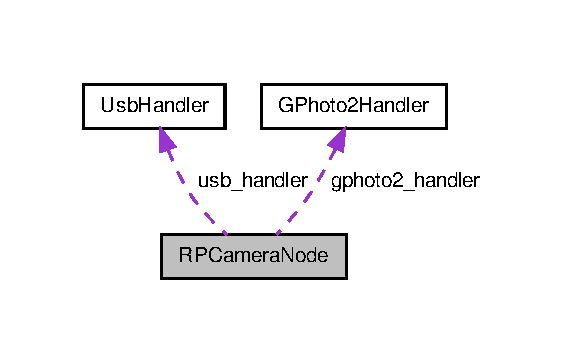
\includegraphics[width=271pt]{class_r_p_camera_node__coll__graph}
\end{center}
\end{figure}
\subsection*{\-Public \-Member \-Functions}
\begin{DoxyCompactItemize}
\item 
\hyperlink{class_r_p_camera_node_a760e6e4ca3230f8c1e74a326a1f3b790}{\-R\-P\-Camera\-Node} (ros\-::\-Node\-Handle \&\hyperlink{class_r_p_camera_node_a258bd2f067f146b88e9f7463f3ef9f3d}{node})
\end{DoxyCompactItemize}
\subsection*{\-Private \-Member \-Functions}
\begin{DoxyCompactItemize}
\item 
bool \hyperlink{class_r_p_camera_node_af1cef4948433c283d26e0aaaf33523bd}{take\-Photo} (rp\-\_\-camera\-::\-Photo\-Service\-::\-Request \&request, rp\-\_\-camera\-::\-Photo\-Service\-::\-Response \&response)
\item 
void \hyperlink{class_r_p_camera_node_a20039ac6f9da622c04ca54bb68fd99f3}{get\-Overridable\-Parameters} ()
\end{DoxyCompactItemize}
\subsection*{\-Private \-Attributes}
\begin{DoxyCompactItemize}
\item 
ros\-::\-Node\-Handle \& \hyperlink{class_r_p_camera_node_a258bd2f067f146b88e9f7463f3ef9f3d}{node}
\item 
ros\-::\-Service\-Server \hyperlink{class_r_p_camera_node_ac8cd380063cf5cc9db19a74845e3f008}{photo\-\_\-service}
\item 
\hyperlink{class_g_photo2_handler}{\-G\-Photo2\-Handler} \hyperlink{class_r_p_camera_node_a15ea1a7dedfc8bca967f1dfd67dc544f}{gphoto2\-\_\-handler}
\item 
\hyperlink{class_usb_handler}{\-Usb\-Handler} \hyperlink{class_r_p_camera_node_aba586a055ce660b850a578150aae1eb7}{usb\-\_\-handler}
\item 
bool \hyperlink{class_r_p_camera_node_ad7b447a8e9d4de116d8407da10750a93}{\-F\-L\-A\-S\-H\-\_\-\-A\-U\-T\-O\-M\-A\-T\-I\-C}
\item 
bool \hyperlink{class_r_p_camera_node_af56a202a81ef4884fb5ce455bb288f42}{\-F\-L\-A\-S\-H\-\_\-\-E\-N\-A\-B\-L\-E\-D}
\item 
std\-::string \hyperlink{class_r_p_camera_node_a5d6be82d1ecbd5cd8dab19c863c8df05}{\-U\-S\-B\-\_\-\-D\-E\-V\-I\-C\-E}
\item 
bool \hyperlink{class_r_p_camera_node_a48ca485f3692b562413f1be1c6fa4952}{\-U\-S\-B\-\_\-\-R\-E\-S\-E\-T\-\_\-\-E\-N\-A\-B\-L\-E\-D}
\end{DoxyCompactItemize}


\subsection{\-Detailed \-Description}
\-Robot photographer's node which takes the pictures using the photographic camera via the gphoto2 library. 

\begin{DoxyCopyright}{\-Copyright}
\-Manfredas \-Zabarauskas, 2013. \-All rights reserved. \-This project is released under \-C\-C \-B\-Y-\/\-N\-C-\/\-S\-A (\-Creative \-Commons \-Attribution-\/\-Non\-Commercial-\/\-Share\-Alike) license. 
\end{DoxyCopyright}


\-Definition at line 24 of file camera.\-hpp.



\subsection{\-Constructor \& \-Destructor \-Documentation}
\hypertarget{class_r_p_camera_node_a760e6e4ca3230f8c1e74a326a1f3b790}{\index{\-R\-P\-Camera\-Node@{\-R\-P\-Camera\-Node}!\-R\-P\-Camera\-Node@{\-R\-P\-Camera\-Node}}
\index{\-R\-P\-Camera\-Node@{\-R\-P\-Camera\-Node}!RPCameraNode@{\-R\-P\-Camera\-Node}}
\subsubsection[{\-R\-P\-Camera\-Node}]{\setlength{\rightskip}{0pt plus 5cm}{\bf \-R\-P\-Camera\-Node\-::\-R\-P\-Camera\-Node} (
\begin{DoxyParamCaption}
\item[{ros\-::\-Node\-Handle \&}]{node}
\end{DoxyParamCaption}
)}}\label{class_r_p_camera_node_a760e6e4ca3230f8c1e74a326a1f3b790}
\-Default photographic camera node's constructor. 
\begin{DoxyParams}{\-Parameters}
{\em node} & \-Handle to \-R\-O\-S node. \\
\hline
\end{DoxyParams}


\-Definition at line 20 of file camera.\-cpp.



\subsection{\-Member \-Function \-Documentation}
\hypertarget{class_r_p_camera_node_a20039ac6f9da622c04ca54bb68fd99f3}{\index{\-R\-P\-Camera\-Node@{\-R\-P\-Camera\-Node}!get\-Overridable\-Parameters@{get\-Overridable\-Parameters}}
\index{get\-Overridable\-Parameters@{get\-Overridable\-Parameters}!RPCameraNode@{\-R\-P\-Camera\-Node}}
\subsubsection[{get\-Overridable\-Parameters}]{\setlength{\rightskip}{0pt plus 5cm}void {\bf \-R\-P\-Camera\-Node\-::get\-Overridable\-Parameters} (
\begin{DoxyParamCaption}
{}
\end{DoxyParamCaption}
)\hspace{0.3cm}{\ttfamily  \mbox{[}private\mbox{]}}}}\label{class_r_p_camera_node_a20039ac6f9da622c04ca54bb68fd99f3}
\-Gets overridable parameters from the parameter server. 

\-Definition at line 46 of file camera.\-cpp.

\hypertarget{class_r_p_camera_node_af1cef4948433c283d26e0aaaf33523bd}{\index{\-R\-P\-Camera\-Node@{\-R\-P\-Camera\-Node}!take\-Photo@{take\-Photo}}
\index{take\-Photo@{take\-Photo}!RPCameraNode@{\-R\-P\-Camera\-Node}}
\subsubsection[{take\-Photo}]{\setlength{\rightskip}{0pt plus 5cm}bool {\bf \-R\-P\-Camera\-Node\-::take\-Photo} (
\begin{DoxyParamCaption}
\item[{rp\-\_\-camera\-::\-Photo\-Service\-::\-Request \&}]{request, }
\item[{rp\-\_\-camera\-::\-Photo\-Service\-::\-Response \&}]{response}
\end{DoxyParamCaption}
)\hspace{0.3cm}{\ttfamily  \mbox{[}private\mbox{]}}}}\label{class_r_p_camera_node_af1cef4948433c283d26e0aaaf33523bd}
\-Callback for the \char`\"{}photograph taking\char`\"{} \-R\-O\-S service request. 
\begin{DoxyParams}{\-Parameters}
{\em request} & \-Empty \-R\-O\-S service request. \\
\hline
{\em response} & \-R\-O\-S photo service response, containing the file name of the taken picture. \\
\hline
\end{DoxyParams}
\begin{DoxyReturn}{\-Returns}
\-Operation's success status. 
\end{DoxyReturn}


\-Definition at line 55 of file camera.\-cpp.



\subsection{\-Member \-Data \-Documentation}
\hypertarget{class_r_p_camera_node_ad7b447a8e9d4de116d8407da10750a93}{\index{\-R\-P\-Camera\-Node@{\-R\-P\-Camera\-Node}!\-F\-L\-A\-S\-H\-\_\-\-A\-U\-T\-O\-M\-A\-T\-I\-C@{\-F\-L\-A\-S\-H\-\_\-\-A\-U\-T\-O\-M\-A\-T\-I\-C}}
\index{\-F\-L\-A\-S\-H\-\_\-\-A\-U\-T\-O\-M\-A\-T\-I\-C@{\-F\-L\-A\-S\-H\-\_\-\-A\-U\-T\-O\-M\-A\-T\-I\-C}!RPCameraNode@{\-R\-P\-Camera\-Node}}
\subsubsection[{\-F\-L\-A\-S\-H\-\_\-\-A\-U\-T\-O\-M\-A\-T\-I\-C}]{\setlength{\rightskip}{0pt plus 5cm}bool {\bf \-R\-P\-Camera\-Node\-::\-F\-L\-A\-S\-H\-\_\-\-A\-U\-T\-O\-M\-A\-T\-I\-C}\hspace{0.3cm}{\ttfamily  \mbox{[}private\mbox{]}}}}\label{class_r_p_camera_node_ad7b447a8e9d4de116d8407da10750a93}
\-Automatic flash overridable parameter (\-O\-P). 

\-Definition at line 34 of file camera.\-hpp.

\hypertarget{class_r_p_camera_node_af56a202a81ef4884fb5ce455bb288f42}{\index{\-R\-P\-Camera\-Node@{\-R\-P\-Camera\-Node}!\-F\-L\-A\-S\-H\-\_\-\-E\-N\-A\-B\-L\-E\-D@{\-F\-L\-A\-S\-H\-\_\-\-E\-N\-A\-B\-L\-E\-D}}
\index{\-F\-L\-A\-S\-H\-\_\-\-E\-N\-A\-B\-L\-E\-D@{\-F\-L\-A\-S\-H\-\_\-\-E\-N\-A\-B\-L\-E\-D}!RPCameraNode@{\-R\-P\-Camera\-Node}}
\subsubsection[{\-F\-L\-A\-S\-H\-\_\-\-E\-N\-A\-B\-L\-E\-D}]{\setlength{\rightskip}{0pt plus 5cm}bool {\bf \-R\-P\-Camera\-Node\-::\-F\-L\-A\-S\-H\-\_\-\-E\-N\-A\-B\-L\-E\-D}\hspace{0.3cm}{\ttfamily  \mbox{[}private\mbox{]}}}}\label{class_r_p_camera_node_af56a202a81ef4884fb5ce455bb288f42}
\-Flash enabled/disabled flag \-O\-P. 

\-Definition at line 35 of file camera.\-hpp.

\hypertarget{class_r_p_camera_node_a15ea1a7dedfc8bca967f1dfd67dc544f}{\index{\-R\-P\-Camera\-Node@{\-R\-P\-Camera\-Node}!gphoto2\-\_\-handler@{gphoto2\-\_\-handler}}
\index{gphoto2\-\_\-handler@{gphoto2\-\_\-handler}!RPCameraNode@{\-R\-P\-Camera\-Node}}
\subsubsection[{gphoto2\-\_\-handler}]{\setlength{\rightskip}{0pt plus 5cm}{\bf \-G\-Photo2\-Handler} {\bf \-R\-P\-Camera\-Node\-::gphoto2\-\_\-handler}\hspace{0.3cm}{\ttfamily  \mbox{[}private\mbox{]}}}}\label{class_r_p_camera_node_a15ea1a7dedfc8bca967f1dfd67dc544f}
\-G\-Photo2 handler. 

\-Definition at line 31 of file camera.\-hpp.

\hypertarget{class_r_p_camera_node_a258bd2f067f146b88e9f7463f3ef9f3d}{\index{\-R\-P\-Camera\-Node@{\-R\-P\-Camera\-Node}!node@{node}}
\index{node@{node}!RPCameraNode@{\-R\-P\-Camera\-Node}}
\subsubsection[{node}]{\setlength{\rightskip}{0pt plus 5cm}ros\-::\-Node\-Handle\& {\bf \-R\-P\-Camera\-Node\-::node}\hspace{0.3cm}{\ttfamily  \mbox{[}private\mbox{]}}}}\label{class_r_p_camera_node_a258bd2f067f146b88e9f7463f3ef9f3d}
\-Node's handle. 

\-Definition at line 27 of file camera.\-hpp.

\hypertarget{class_r_p_camera_node_ac8cd380063cf5cc9db19a74845e3f008}{\index{\-R\-P\-Camera\-Node@{\-R\-P\-Camera\-Node}!photo\-\_\-service@{photo\-\_\-service}}
\index{photo\-\_\-service@{photo\-\_\-service}!RPCameraNode@{\-R\-P\-Camera\-Node}}
\subsubsection[{photo\-\_\-service}]{\setlength{\rightskip}{0pt plus 5cm}ros\-::\-Service\-Server {\bf \-R\-P\-Camera\-Node\-::photo\-\_\-service}\hspace{0.3cm}{\ttfamily  \mbox{[}private\mbox{]}}}}\label{class_r_p_camera_node_ac8cd380063cf5cc9db19a74845e3f008}
\-Advertised photo service. 

\-Definition at line 29 of file camera.\-hpp.

\hypertarget{class_r_p_camera_node_a5d6be82d1ecbd5cd8dab19c863c8df05}{\index{\-R\-P\-Camera\-Node@{\-R\-P\-Camera\-Node}!\-U\-S\-B\-\_\-\-D\-E\-V\-I\-C\-E@{\-U\-S\-B\-\_\-\-D\-E\-V\-I\-C\-E}}
\index{\-U\-S\-B\-\_\-\-D\-E\-V\-I\-C\-E@{\-U\-S\-B\-\_\-\-D\-E\-V\-I\-C\-E}!RPCameraNode@{\-R\-P\-Camera\-Node}}
\subsubsection[{\-U\-S\-B\-\_\-\-D\-E\-V\-I\-C\-E}]{\setlength{\rightskip}{0pt plus 5cm}std\-::string {\bf \-R\-P\-Camera\-Node\-::\-U\-S\-B\-\_\-\-D\-E\-V\-I\-C\-E}\hspace{0.3cm}{\ttfamily  \mbox{[}private\mbox{]}}}}\label{class_r_p_camera_node_a5d6be82d1ecbd5cd8dab19c863c8df05}
\-U\-S\-B device path \-O\-P. 

\-Definition at line 36 of file camera.\-hpp.

\hypertarget{class_r_p_camera_node_aba586a055ce660b850a578150aae1eb7}{\index{\-R\-P\-Camera\-Node@{\-R\-P\-Camera\-Node}!usb\-\_\-handler@{usb\-\_\-handler}}
\index{usb\-\_\-handler@{usb\-\_\-handler}!RPCameraNode@{\-R\-P\-Camera\-Node}}
\subsubsection[{usb\-\_\-handler}]{\setlength{\rightskip}{0pt plus 5cm}{\bf \-Usb\-Handler} {\bf \-R\-P\-Camera\-Node\-::usb\-\_\-handler}\hspace{0.3cm}{\ttfamily  \mbox{[}private\mbox{]}}}}\label{class_r_p_camera_node_aba586a055ce660b850a578150aae1eb7}
\-U\-S\-B reset handler. 

\-Definition at line 32 of file camera.\-hpp.

\hypertarget{class_r_p_camera_node_a48ca485f3692b562413f1be1c6fa4952}{\index{\-R\-P\-Camera\-Node@{\-R\-P\-Camera\-Node}!\-U\-S\-B\-\_\-\-R\-E\-S\-E\-T\-\_\-\-E\-N\-A\-B\-L\-E\-D@{\-U\-S\-B\-\_\-\-R\-E\-S\-E\-T\-\_\-\-E\-N\-A\-B\-L\-E\-D}}
\index{\-U\-S\-B\-\_\-\-R\-E\-S\-E\-T\-\_\-\-E\-N\-A\-B\-L\-E\-D@{\-U\-S\-B\-\_\-\-R\-E\-S\-E\-T\-\_\-\-E\-N\-A\-B\-L\-E\-D}!RPCameraNode@{\-R\-P\-Camera\-Node}}
\subsubsection[{\-U\-S\-B\-\_\-\-R\-E\-S\-E\-T\-\_\-\-E\-N\-A\-B\-L\-E\-D}]{\setlength{\rightskip}{0pt plus 5cm}bool {\bf \-R\-P\-Camera\-Node\-::\-U\-S\-B\-\_\-\-R\-E\-S\-E\-T\-\_\-\-E\-N\-A\-B\-L\-E\-D}\hspace{0.3cm}{\ttfamily  \mbox{[}private\mbox{]}}}}\label{class_r_p_camera_node_a48ca485f3692b562413f1be1c6fa4952}
\-U\-S\-B device reset enabled/disabled flag \-O\-P. 

\-Definition at line 37 of file camera.\-hpp.



\-The documentation for this class was generated from the following files\-:\begin{DoxyCompactItemize}
\item 
rp\-\_\-camera/include/camera.\-hpp\item 
rp\-\_\-camera/src/camera.\-cpp\end{DoxyCompactItemize}

\hypertarget{class_r_p_color_face_detector}{\section{\-R\-P\-Color\-Face\-Detector \-Class \-Reference}
\label{class_r_p_color_face_detector}\index{\-R\-P\-Color\-Face\-Detector@{\-R\-P\-Color\-Face\-Detector}}
}


\-Face detector in colour images, based on \-Viola and \-Jones (2001) face detector implementation in \-Open\-C\-V.  




{\ttfamily \#include $<$color\-\_\-face\-\_\-detector.\-hpp$>$}

\subsection*{\-Public \-Member \-Functions}
\begin{DoxyCompactItemize}
\item 
\hyperlink{class_r_p_color_face_detector_a2822056221a0a6dd1d5e387c71e0a7dc}{\-R\-P\-Color\-Face\-Detector} (const ros\-::\-Node\-Handle \&node)
\item 
void \hyperlink{class_r_p_color_face_detector_a80d45d6a227ad41f31483a7d85a9bc9a}{detect\-Faces} (const cv\-\_\-bridge\-::\-Cv\-Image\-::\-Const\-Ptr \&input\-\_\-image, std\-::vector$<$ cv\-::\-Rect $>$ \&faces)
\item 
void \hyperlink{class_r_p_color_face_detector_aa156cf14c4cf0f2fe2f58d1c9ce297a7}{detect\-Faces} (const cv\-::\-Mat \&input\-\_\-image, std\-::vector$<$ cv\-::\-Rect $>$ \&faces)
\end{DoxyCompactItemize}
\subsection*{\-Private \-Member \-Functions}
\begin{DoxyCompactItemize}
\item 
void \hyperlink{class_r_p_color_face_detector_ab730fa54b6c1ef6224d6577736970ecc}{get\-Overridable\-Parameters} (const ros\-::\-Node\-Handle \&node)
\end{DoxyCompactItemize}
\subsection*{\-Private \-Attributes}
\begin{DoxyCompactItemize}
\item 
cv\-::\-Cascade\-Classifier \hyperlink{class_r_p_color_face_detector_a4ab7e99e6da2768d2005d573a43d1f30}{frontal\-\_\-cascade}
\item 
cv\-::\-Cascade\-Classifier \hyperlink{class_r_p_color_face_detector_a27f973deeb52ebaa3c9a49a8eace16a5}{profile\-\_\-cascade}
\item 
std\-::string \hyperlink{class_r_p_color_face_detector_a22af60d876ae98cf57f73cdf6ff24d82}{\-F\-A\-C\-E\-\_\-\-D\-E\-T\-E\-C\-T\-O\-R\-\_\-\-F\-R\-O\-N\-T\-A\-L\-\_\-\-C\-A\-S\-C\-A\-D\-E\-\_\-\-P\-A\-T\-H}
\item 
std\-::string \hyperlink{class_r_p_color_face_detector_a21186fee954aa109b73910875f60f7f0}{\-F\-A\-C\-E\-\_\-\-D\-E\-T\-E\-C\-T\-O\-R\-\_\-\-P\-R\-O\-F\-I\-L\-E\-\_\-\-C\-A\-S\-C\-A\-D\-E\-\_\-\-P\-A\-T\-H}
\item 
int \hyperlink{class_r_p_color_face_detector_ae86967285f09aa17afa81dce94642aff}{\-V\-I\-O\-L\-A\-\_\-\-J\-O\-N\-E\-S\-\_\-\-N\-E\-I\-G\-H\-B\-O\-R\-\_\-\-C\-O\-U\-N\-T}
\end{DoxyCompactItemize}


\subsection{\-Detailed \-Description}
\-Face detector in colour images, based on \-Viola and \-Jones (2001) face detector implementation in \-Open\-C\-V. 

\begin{DoxyCopyright}{\-Copyright}
\-Manfredas \-Zabarauskas, 2013. \-All rights reserved. \-This project is released under \-C\-C \-B\-Y-\/\-N\-C-\/\-S\-A (\-Creative \-Commons \-Attribution-\/\-Non\-Commercial-\/\-Share\-Alike) license. 
\end{DoxyCopyright}


\-Definition at line 32 of file color\-\_\-face\-\_\-detector.\-hpp.



\subsection{\-Constructor \& \-Destructor \-Documentation}
\hypertarget{class_r_p_color_face_detector_a2822056221a0a6dd1d5e387c71e0a7dc}{\index{\-R\-P\-Color\-Face\-Detector@{\-R\-P\-Color\-Face\-Detector}!\-R\-P\-Color\-Face\-Detector@{\-R\-P\-Color\-Face\-Detector}}
\index{\-R\-P\-Color\-Face\-Detector@{\-R\-P\-Color\-Face\-Detector}!RPColorFaceDetector@{\-R\-P\-Color\-Face\-Detector}}
\subsubsection[{\-R\-P\-Color\-Face\-Detector}]{\setlength{\rightskip}{0pt plus 5cm}{\bf \-R\-P\-Color\-Face\-Detector\-::\-R\-P\-Color\-Face\-Detector} (
\begin{DoxyParamCaption}
\item[{const ros\-::\-Node\-Handle \&}]{node}
\end{DoxyParamCaption}
)}}\label{class_r_p_color_face_detector_a2822056221a0a6dd1d5e387c71e0a7dc}
\-Default autonomous photography node's constructor. 
\begin{DoxyParams}{\-Parameters}
{\em node} & \-Handle to \-R\-O\-S node.\\
\hline
\end{DoxyParams}
\begin{DoxyCopyright}{\-Copyright}
\-Manfredas \-Zabarauskas, 2013. \-All rights reserved. \-This project is released under \-C\-C \-B\-Y-\/\-N\-C-\/\-S\-A (\-Creative \-Commons \-Attribution-\/\-Non\-Commercial-\/\-Share\-Alike) license. 
\end{DoxyCopyright}


\-Definition at line 12 of file color\-\_\-face\-\_\-detector.\-cpp.



\subsection{\-Member \-Function \-Documentation}
\hypertarget{class_r_p_color_face_detector_a80d45d6a227ad41f31483a7d85a9bc9a}{\index{\-R\-P\-Color\-Face\-Detector@{\-R\-P\-Color\-Face\-Detector}!detect\-Faces@{detect\-Faces}}
\index{detect\-Faces@{detect\-Faces}!RPColorFaceDetector@{\-R\-P\-Color\-Face\-Detector}}
\subsubsection[{detect\-Faces}]{\setlength{\rightskip}{0pt plus 5cm}void {\bf \-R\-P\-Color\-Face\-Detector\-::detect\-Faces} (
\begin{DoxyParamCaption}
\item[{const cv\-\_\-bridge\-::\-Cv\-Image\-::\-Const\-Ptr \&}]{input\-\_\-image, }
\item[{std\-::vector$<$ cv\-::\-Rect $>$ \&}]{faces}
\end{DoxyParamCaption}
)}}\label{class_r_p_color_face_detector_a80d45d6a227ad41f31483a7d85a9bc9a}
\-Detects faces in a given \-R\-G\-B image. 
\begin{DoxyParams}{\-Parameters}
{\em input\-\_\-image} & \-Input \-R\-G\-B image. \\
\hline
{\em faces} & \-Deteted faces. \\
\hline
\end{DoxyParams}


\-Definition at line 62 of file color\-\_\-face\-\_\-detector.\-cpp.

\hypertarget{class_r_p_color_face_detector_aa156cf14c4cf0f2fe2f58d1c9ce297a7}{\index{\-R\-P\-Color\-Face\-Detector@{\-R\-P\-Color\-Face\-Detector}!detect\-Faces@{detect\-Faces}}
\index{detect\-Faces@{detect\-Faces}!RPColorFaceDetector@{\-R\-P\-Color\-Face\-Detector}}
\subsubsection[{detect\-Faces}]{\setlength{\rightskip}{0pt plus 5cm}void {\bf \-R\-P\-Color\-Face\-Detector\-::detect\-Faces} (
\begin{DoxyParamCaption}
\item[{const cv\-::\-Mat \&}]{input\-\_\-image, }
\item[{std\-::vector$<$ cv\-::\-Rect $>$ \&}]{faces}
\end{DoxyParamCaption}
)}}\label{class_r_p_color_face_detector_aa156cf14c4cf0f2fe2f58d1c9ce297a7}
\-Detects faces in a given \-Open\-C\-V matrix representation of an image (in \-C\-V\-\_\-8\-U\-C3 format, i.\-e. using 8 unsigned bits to represent each of the \-R, \-G and \-B color channels). 
\begin{DoxyParams}{\-Parameters}
{\em input\-\_\-image} & \-Input image matrix in \-C\-V\-\_\-8\-U\-C3 format. \\
\hline
{\em faces} & \-Deteted faces. \\
\hline
\end{DoxyParams}


\-Definition at line 40 of file color\-\_\-face\-\_\-detector.\-cpp.

\hypertarget{class_r_p_color_face_detector_ab730fa54b6c1ef6224d6577736970ecc}{\index{\-R\-P\-Color\-Face\-Detector@{\-R\-P\-Color\-Face\-Detector}!get\-Overridable\-Parameters@{get\-Overridable\-Parameters}}
\index{get\-Overridable\-Parameters@{get\-Overridable\-Parameters}!RPColorFaceDetector@{\-R\-P\-Color\-Face\-Detector}}
\subsubsection[{get\-Overridable\-Parameters}]{\setlength{\rightskip}{0pt plus 5cm}void {\bf \-R\-P\-Color\-Face\-Detector\-::get\-Overridable\-Parameters} (
\begin{DoxyParamCaption}
\item[{const ros\-::\-Node\-Handle \&}]{node}
\end{DoxyParamCaption}
)\hspace{0.3cm}{\ttfamily  \mbox{[}private\mbox{]}}}}\label{class_r_p_color_face_detector_ab730fa54b6c1ef6224d6577736970ecc}
\-Gets the overridable parameters from the parameter server. 
\begin{DoxyParams}{\-Parameters}
{\em node} & \-Handle to \-R\-O\-S node. \\
\hline
\end{DoxyParams}


\-Definition at line 32 of file color\-\_\-face\-\_\-detector.\-cpp.



\subsection{\-Member \-Data \-Documentation}
\hypertarget{class_r_p_color_face_detector_a22af60d876ae98cf57f73cdf6ff24d82}{\index{\-R\-P\-Color\-Face\-Detector@{\-R\-P\-Color\-Face\-Detector}!\-F\-A\-C\-E\-\_\-\-D\-E\-T\-E\-C\-T\-O\-R\-\_\-\-F\-R\-O\-N\-T\-A\-L\-\_\-\-C\-A\-S\-C\-A\-D\-E\-\_\-\-P\-A\-T\-H@{\-F\-A\-C\-E\-\_\-\-D\-E\-T\-E\-C\-T\-O\-R\-\_\-\-F\-R\-O\-N\-T\-A\-L\-\_\-\-C\-A\-S\-C\-A\-D\-E\-\_\-\-P\-A\-T\-H}}
\index{\-F\-A\-C\-E\-\_\-\-D\-E\-T\-E\-C\-T\-O\-R\-\_\-\-F\-R\-O\-N\-T\-A\-L\-\_\-\-C\-A\-S\-C\-A\-D\-E\-\_\-\-P\-A\-T\-H@{\-F\-A\-C\-E\-\_\-\-D\-E\-T\-E\-C\-T\-O\-R\-\_\-\-F\-R\-O\-N\-T\-A\-L\-\_\-\-C\-A\-S\-C\-A\-D\-E\-\_\-\-P\-A\-T\-H}!RPColorFaceDetector@{\-R\-P\-Color\-Face\-Detector}}
\subsubsection[{\-F\-A\-C\-E\-\_\-\-D\-E\-T\-E\-C\-T\-O\-R\-\_\-\-F\-R\-O\-N\-T\-A\-L\-\_\-\-C\-A\-S\-C\-A\-D\-E\-\_\-\-P\-A\-T\-H}]{\setlength{\rightskip}{0pt plus 5cm}std\-::string {\bf \-R\-P\-Color\-Face\-Detector\-::\-F\-A\-C\-E\-\_\-\-D\-E\-T\-E\-C\-T\-O\-R\-\_\-\-F\-R\-O\-N\-T\-A\-L\-\_\-\-C\-A\-S\-C\-A\-D\-E\-\_\-\-P\-A\-T\-H}\hspace{0.3cm}{\ttfamily  \mbox{[}private\mbox{]}}}}\label{class_r_p_color_face_detector_a22af60d876ae98cf57f73cdf6ff24d82}
\-Frontal face detector cascade file path. 

\-Definition at line 40 of file color\-\_\-face\-\_\-detector.\-hpp.

\hypertarget{class_r_p_color_face_detector_a21186fee954aa109b73910875f60f7f0}{\index{\-R\-P\-Color\-Face\-Detector@{\-R\-P\-Color\-Face\-Detector}!\-F\-A\-C\-E\-\_\-\-D\-E\-T\-E\-C\-T\-O\-R\-\_\-\-P\-R\-O\-F\-I\-L\-E\-\_\-\-C\-A\-S\-C\-A\-D\-E\-\_\-\-P\-A\-T\-H@{\-F\-A\-C\-E\-\_\-\-D\-E\-T\-E\-C\-T\-O\-R\-\_\-\-P\-R\-O\-F\-I\-L\-E\-\_\-\-C\-A\-S\-C\-A\-D\-E\-\_\-\-P\-A\-T\-H}}
\index{\-F\-A\-C\-E\-\_\-\-D\-E\-T\-E\-C\-T\-O\-R\-\_\-\-P\-R\-O\-F\-I\-L\-E\-\_\-\-C\-A\-S\-C\-A\-D\-E\-\_\-\-P\-A\-T\-H@{\-F\-A\-C\-E\-\_\-\-D\-E\-T\-E\-C\-T\-O\-R\-\_\-\-P\-R\-O\-F\-I\-L\-E\-\_\-\-C\-A\-S\-C\-A\-D\-E\-\_\-\-P\-A\-T\-H}!RPColorFaceDetector@{\-R\-P\-Color\-Face\-Detector}}
\subsubsection[{\-F\-A\-C\-E\-\_\-\-D\-E\-T\-E\-C\-T\-O\-R\-\_\-\-P\-R\-O\-F\-I\-L\-E\-\_\-\-C\-A\-S\-C\-A\-D\-E\-\_\-\-P\-A\-T\-H}]{\setlength{\rightskip}{0pt plus 5cm}std\-::string {\bf \-R\-P\-Color\-Face\-Detector\-::\-F\-A\-C\-E\-\_\-\-D\-E\-T\-E\-C\-T\-O\-R\-\_\-\-P\-R\-O\-F\-I\-L\-E\-\_\-\-C\-A\-S\-C\-A\-D\-E\-\_\-\-P\-A\-T\-H}\hspace{0.3cm}{\ttfamily  \mbox{[}private\mbox{]}}}}\label{class_r_p_color_face_detector_a21186fee954aa109b73910875f60f7f0}
\-Profile face detector cascade file path. 

\-Definition at line 41 of file color\-\_\-face\-\_\-detector.\-hpp.

\hypertarget{class_r_p_color_face_detector_a4ab7e99e6da2768d2005d573a43d1f30}{\index{\-R\-P\-Color\-Face\-Detector@{\-R\-P\-Color\-Face\-Detector}!frontal\-\_\-cascade@{frontal\-\_\-cascade}}
\index{frontal\-\_\-cascade@{frontal\-\_\-cascade}!RPColorFaceDetector@{\-R\-P\-Color\-Face\-Detector}}
\subsubsection[{frontal\-\_\-cascade}]{\setlength{\rightskip}{0pt plus 5cm}cv\-::\-Cascade\-Classifier {\bf \-R\-P\-Color\-Face\-Detector\-::frontal\-\_\-cascade}\hspace{0.3cm}{\ttfamily  \mbox{[}private\mbox{]}}}}\label{class_r_p_color_face_detector_a4ab7e99e6da2768d2005d573a43d1f30}
\-Frontal face detector cascade. 

\-Definition at line 36 of file color\-\_\-face\-\_\-detector.\-hpp.

\hypertarget{class_r_p_color_face_detector_a27f973deeb52ebaa3c9a49a8eace16a5}{\index{\-R\-P\-Color\-Face\-Detector@{\-R\-P\-Color\-Face\-Detector}!profile\-\_\-cascade@{profile\-\_\-cascade}}
\index{profile\-\_\-cascade@{profile\-\_\-cascade}!RPColorFaceDetector@{\-R\-P\-Color\-Face\-Detector}}
\subsubsection[{profile\-\_\-cascade}]{\setlength{\rightskip}{0pt plus 5cm}cv\-::\-Cascade\-Classifier {\bf \-R\-P\-Color\-Face\-Detector\-::profile\-\_\-cascade}\hspace{0.3cm}{\ttfamily  \mbox{[}private\mbox{]}}}}\label{class_r_p_color_face_detector_a27f973deeb52ebaa3c9a49a8eace16a5}
\-Profile face detector cascade. 

\-Definition at line 37 of file color\-\_\-face\-\_\-detector.\-hpp.

\hypertarget{class_r_p_color_face_detector_ae86967285f09aa17afa81dce94642aff}{\index{\-R\-P\-Color\-Face\-Detector@{\-R\-P\-Color\-Face\-Detector}!\-V\-I\-O\-L\-A\-\_\-\-J\-O\-N\-E\-S\-\_\-\-N\-E\-I\-G\-H\-B\-O\-R\-\_\-\-C\-O\-U\-N\-T@{\-V\-I\-O\-L\-A\-\_\-\-J\-O\-N\-E\-S\-\_\-\-N\-E\-I\-G\-H\-B\-O\-R\-\_\-\-C\-O\-U\-N\-T}}
\index{\-V\-I\-O\-L\-A\-\_\-\-J\-O\-N\-E\-S\-\_\-\-N\-E\-I\-G\-H\-B\-O\-R\-\_\-\-C\-O\-U\-N\-T@{\-V\-I\-O\-L\-A\-\_\-\-J\-O\-N\-E\-S\-\_\-\-N\-E\-I\-G\-H\-B\-O\-R\-\_\-\-C\-O\-U\-N\-T}!RPColorFaceDetector@{\-R\-P\-Color\-Face\-Detector}}
\subsubsection[{\-V\-I\-O\-L\-A\-\_\-\-J\-O\-N\-E\-S\-\_\-\-N\-E\-I\-G\-H\-B\-O\-R\-\_\-\-C\-O\-U\-N\-T}]{\setlength{\rightskip}{0pt plus 5cm}int {\bf \-R\-P\-Color\-Face\-Detector\-::\-V\-I\-O\-L\-A\-\_\-\-J\-O\-N\-E\-S\-\_\-\-N\-E\-I\-G\-H\-B\-O\-R\-\_\-\-C\-O\-U\-N\-T}\hspace{0.3cm}{\ttfamily  \mbox{[}private\mbox{]}}}}\label{class_r_p_color_face_detector_ae86967285f09aa17afa81dce94642aff}
\-Minimal neighbor count required for \-Viola-\/\-Jones face detectors to register a face detection. 

\-Definition at line 42 of file color\-\_\-face\-\_\-detector.\-hpp.



\-The documentation for this class was generated from the following files\-:\begin{DoxyCompactItemize}
\item 
rp\-\_\-head\-\_\-tracking/include/color\-\_\-face\-\_\-detector.\-hpp\item 
rp\-\_\-head\-\_\-tracking/src/color\-\_\-face\-\_\-detector.\-cpp\end{DoxyCompactItemize}

\hypertarget{class_r_p_color_image_processor}{\section{\-R\-P\-Color\-Image\-Processor \-Class \-Reference}
\label{class_r_p_color_image_processor}\index{\-R\-P\-Color\-Image\-Processor@{\-R\-P\-Color\-Image\-Processor}}
}


\-Color image processor class, which provides implementations for simple color image manipulation tasks.  




{\ttfamily \#include $<$color\-\_\-image\-\_\-processor.\-hpp$>$}

\subsection*{\-Public \-Member \-Functions}
\begin{DoxyCompactItemize}
\item 
void \hyperlink{class_r_p_color_image_processor_accdef8184c373b30dd97e7fb4aea91b9}{convert\-Color\-Image\-To\-Render\-Image} (const cv\-\_\-bridge\-::\-Cv\-Image\-::\-Const\-Ptr \&color\-\_\-image, cv\-::\-Mat \&render\-\_\-image)
\item 
void \hyperlink{class_r_p_color_image_processor_ac2571f36fd53d8725a60a311a4124430}{convert\-Color\-Image\-To\-Backpropagation\-Image} (const cv\-\_\-bridge\-::\-Cv\-Image\-::\-Const\-Ptr \&color\-\_\-image, cv\-::\-Mat \&render\-\_\-image, \hyperlink{class_r_p_bayesian_skin_classifier}{\-R\-P\-Bayesian\-Skin\-Classifier} \&skin\-\_\-classifier, const int skin\-\_\-likelihood\-\_\-ratio\-\_\-minimum)
\item 
void \hyperlink{class_r_p_color_image_processor_a1766a497e20c8e375a3c89ff3b259155}{create\-Skin\-Hue\-Training\-Example} (cv\-::\-Rect \&face\-\_\-rectangle, const cv\-\_\-bridge\-::\-Cv\-Image\-::\-Const\-Ptr \&color\-\_\-image, std\-::vector$<$ double $>$ \&hue\-\_\-histogram)
\item 
void \hyperlink{class_r_p_color_image_processor_a4f59934cb9fb920b76a621ebe94333c8}{create\-Non\-Skin\-Hue\-Training\-Example} (cv\-::\-Rect \&face\-\_\-rectangle, const cv\-\_\-bridge\-::\-Cv\-Image\-::\-Const\-Ptr \&color\-\_\-image, std\-::vector$<$ double $>$ \&hue\-\_\-histogram)
\item 
void \hyperlink{class_r_p_color_image_processor_a137e06bfcf21db64a099c0c74086c7ee}{create\-Histogram} (const cv\-::\-Mat \&histogram\-\_\-region, std\-::vector$<$ double $>$ \&histogram)
\end{DoxyCompactItemize}


\subsection{\-Detailed \-Description}
\-Color image processor class, which provides implementations for simple color image manipulation tasks. 

\begin{DoxyCopyright}{\-Copyright}
\-Manfredas \-Zabarauskas, 2013. \-All rights reserved. \-This project is released under \-C\-C \-B\-Y-\/\-N\-C-\/\-S\-A (\-Creative \-Commons \-Attribution-\/\-Non\-Commercial-\/\-Share\-Alike) license. 
\end{DoxyCopyright}


\-Definition at line 24 of file color\-\_\-image\-\_\-processor.\-hpp.



\subsection{\-Member \-Function \-Documentation}
\hypertarget{class_r_p_color_image_processor_ac2571f36fd53d8725a60a311a4124430}{\index{\-R\-P\-Color\-Image\-Processor@{\-R\-P\-Color\-Image\-Processor}!convert\-Color\-Image\-To\-Backpropagation\-Image@{convert\-Color\-Image\-To\-Backpropagation\-Image}}
\index{convert\-Color\-Image\-To\-Backpropagation\-Image@{convert\-Color\-Image\-To\-Backpropagation\-Image}!RPColorImageProcessor@{\-R\-P\-Color\-Image\-Processor}}
\subsubsection[{convert\-Color\-Image\-To\-Backpropagation\-Image}]{\setlength{\rightskip}{0pt plus 5cm}void {\bf \-R\-P\-Color\-Image\-Processor\-::convert\-Color\-Image\-To\-Backpropagation\-Image} (
\begin{DoxyParamCaption}
\item[{const cv\-\_\-bridge\-::\-Cv\-Image\-::\-Const\-Ptr \&}]{color\-\_\-image, }
\item[{cv\-::\-Mat \&}]{render\-\_\-image, }
\item[{{\bf \-R\-P\-Bayesian\-Skin\-Classifier} \&}]{skin\-\_\-classifier, }
\item[{const int}]{skin\-\_\-likelihood\-\_\-ratio\-\_\-minimum}
\end{DoxyParamCaption}
)}}\label{class_r_p_color_image_processor_ac2571f36fd53d8725a60a311a4124430}
\-Converts the color \-R\-G\-B image provided by cv\-\_\-bridge into a backpropagation image, stored in an \-Open\-C\-V matrix. 
\begin{DoxyParams}{\-Parameters}
{\em color\-\_\-image} & \-Input color \-R\-G\-B image from cv\-\_\-bridge. \\
\hline
{\em render\-\_\-image} & \-Backpropagation image stored in an \-Open\-C\-V matrix. \\
\hline
{\em skin\-\_\-classifier} & \-Bayesian skin classifier. \\
\hline
{\em skin\-\_\-likelihood\-\_\-ratio\-\_\-minimum} & \-Minimum skin likelihood ratio (used as a threshold). \\
\hline
\end{DoxyParams}


\-Definition at line 20 of file color\-\_\-image\-\_\-processor.\-cpp.

\hypertarget{class_r_p_color_image_processor_accdef8184c373b30dd97e7fb4aea91b9}{\index{\-R\-P\-Color\-Image\-Processor@{\-R\-P\-Color\-Image\-Processor}!convert\-Color\-Image\-To\-Render\-Image@{convert\-Color\-Image\-To\-Render\-Image}}
\index{convert\-Color\-Image\-To\-Render\-Image@{convert\-Color\-Image\-To\-Render\-Image}!RPColorImageProcessor@{\-R\-P\-Color\-Image\-Processor}}
\subsubsection[{convert\-Color\-Image\-To\-Render\-Image}]{\setlength{\rightskip}{0pt plus 5cm}void {\bf \-R\-P\-Color\-Image\-Processor\-::convert\-Color\-Image\-To\-Render\-Image} (
\begin{DoxyParamCaption}
\item[{const cv\-\_\-bridge\-::\-Cv\-Image\-::\-Const\-Ptr \&}]{color\-\_\-image, }
\item[{cv\-::\-Mat \&}]{render\-\_\-image}
\end{DoxyParamCaption}
)}}\label{class_r_p_color_image_processor_accdef8184c373b30dd97e7fb4aea91b9}
\-Copies the color \-R\-G\-B image provided by cv\-\_\-bridge into an \-Open\-C\-V matrix. 
\begin{DoxyParams}{\-Parameters}
{\em color\-\_\-image} & \-Input color \-R\-G\-B image from cv\-\_\-bridge. \\
\hline
{\em render\-\_\-image} & \-Same \-R\-G\-B image copied to an \-Open\-C\-V matrix.\\
\hline
\end{DoxyParams}
\begin{DoxyCopyright}{\-Copyright}
\-Manfredas \-Zabarauskas, 2013. \-All rights reserved. \-This project is released under \-C\-C \-B\-Y-\/\-N\-C-\/\-S\-A (\-Creative \-Commons \-Attribution-\/\-Non\-Commercial-\/\-Share\-Alike) license. 
\end{DoxyCopyright}


\-Definition at line 14 of file color\-\_\-image\-\_\-processor.\-cpp.

\hypertarget{class_r_p_color_image_processor_a137e06bfcf21db64a099c0c74086c7ee}{\index{\-R\-P\-Color\-Image\-Processor@{\-R\-P\-Color\-Image\-Processor}!create\-Histogram@{create\-Histogram}}
\index{create\-Histogram@{create\-Histogram}!RPColorImageProcessor@{\-R\-P\-Color\-Image\-Processor}}
\subsubsection[{create\-Histogram}]{\setlength{\rightskip}{0pt plus 5cm}void {\bf \-R\-P\-Color\-Image\-Processor\-::create\-Histogram} (
\begin{DoxyParamCaption}
\item[{const cv\-::\-Mat \&}]{histogram\-\_\-region, }
\item[{std\-::vector$<$ double $>$ \&}]{histogram}
\end{DoxyParamCaption}
)}}\label{class_r_p_color_image_processor_a137e06bfcf21db64a099c0c74086c7ee}
\-Creates a histogram from a given region in an image. 
\begin{DoxyParams}{\-Parameters}
{\em histogram\-\_\-region} & \-Histogram region in an image. \\
\hline
{\em histogram} & \-Resultant histogram. \\
\hline
\end{DoxyParams}


\-Definition at line 38 of file color\-\_\-image\-\_\-processor.\-cpp.

\hypertarget{class_r_p_color_image_processor_a4f59934cb9fb920b76a621ebe94333c8}{\index{\-R\-P\-Color\-Image\-Processor@{\-R\-P\-Color\-Image\-Processor}!create\-Non\-Skin\-Hue\-Training\-Example@{create\-Non\-Skin\-Hue\-Training\-Example}}
\index{create\-Non\-Skin\-Hue\-Training\-Example@{create\-Non\-Skin\-Hue\-Training\-Example}!RPColorImageProcessor@{\-R\-P\-Color\-Image\-Processor}}
\subsubsection[{create\-Non\-Skin\-Hue\-Training\-Example}]{\setlength{\rightskip}{0pt plus 5cm}void {\bf \-R\-P\-Color\-Image\-Processor\-::create\-Non\-Skin\-Hue\-Training\-Example} (
\begin{DoxyParamCaption}
\item[{cv\-::\-Rect \&}]{face\-\_\-rectangle, }
\item[{const cv\-\_\-bridge\-::\-Cv\-Image\-::\-Const\-Ptr \&}]{color\-\_\-image, }
\item[{std\-::vector$<$ double $>$ \&}]{hue\-\_\-histogram}
\end{DoxyParamCaption}
)}}\label{class_r_p_color_image_processor_a4f59934cb9fb920b76a621ebe94333c8}
\-Creates a non-\/skin hue histogram from a given detected face rectangle in a given color image. 
\begin{DoxyParams}{\-Parameters}
{\em face\-\_\-rectangle} & \-Input detected face rectangle. \\
\hline
{\em color\-\_\-image} & \-Input color image. \\
\hline
{\em hue\-\_\-histogram} & \-Output non-\/skin hue histogram. \\
\hline
\end{DoxyParams}


\-Definition at line 100 of file color\-\_\-image\-\_\-processor.\-cpp.

\hypertarget{class_r_p_color_image_processor_a1766a497e20c8e375a3c89ff3b259155}{\index{\-R\-P\-Color\-Image\-Processor@{\-R\-P\-Color\-Image\-Processor}!create\-Skin\-Hue\-Training\-Example@{create\-Skin\-Hue\-Training\-Example}}
\index{create\-Skin\-Hue\-Training\-Example@{create\-Skin\-Hue\-Training\-Example}!RPColorImageProcessor@{\-R\-P\-Color\-Image\-Processor}}
\subsubsection[{create\-Skin\-Hue\-Training\-Example}]{\setlength{\rightskip}{0pt plus 5cm}void {\bf \-R\-P\-Color\-Image\-Processor\-::create\-Skin\-Hue\-Training\-Example} (
\begin{DoxyParamCaption}
\item[{cv\-::\-Rect \&}]{face\-\_\-rectangle, }
\item[{const cv\-\_\-bridge\-::\-Cv\-Image\-::\-Const\-Ptr \&}]{color\-\_\-image, }
\item[{std\-::vector$<$ double $>$ \&}]{hue\-\_\-histogram}
\end{DoxyParamCaption}
)}}\label{class_r_p_color_image_processor_a1766a497e20c8e375a3c89ff3b259155}
\-Creates a skin hue histogram from a given detected face rectangle in a given color image. 
\begin{DoxyParams}{\-Parameters}
{\em face\-\_\-rectangle} & \-Input detected face rectangle. \\
\hline
{\em color\-\_\-image} & \-Input color image. \\
\hline
{\em hue\-\_\-histogram} & \-Output skin hue histogram. \\
\hline
\end{DoxyParams}


\-Definition at line 69 of file color\-\_\-image\-\_\-processor.\-cpp.



\-The documentation for this class was generated from the following files\-:\begin{DoxyCompactItemize}
\item 
rp\-\_\-head\-\_\-tracking/include/color\-\_\-image\-\_\-processor.\-hpp\item 
rp\-\_\-head\-\_\-tracking/src/color\-\_\-image\-\_\-processor.\-cpp\end{DoxyCompactItemize}

\hypertarget{class_r_p_depth_head_detector}{\section{\-R\-P\-Depth\-Head\-Detector \-Class \-Reference}
\label{class_r_p_depth_head_detector}\index{\-R\-P\-Depth\-Head\-Detector@{\-R\-P\-Depth\-Head\-Detector}}
}


\hyperlink{struct_head}{\-Head} detector from depth images.  




{\ttfamily \#include $<$depth\-\_\-head\-\_\-detector.\-hpp$>$}

\subsection*{\-Classes}
\begin{DoxyCompactItemize}
\item 
struct \hyperlink{struct_r_p_depth_head_detector_1_1_r_p_detected_head}{\-R\-P\-Detected\-Head}
\end{DoxyCompactItemize}
\subsection*{\-Public \-Member \-Functions}
\begin{DoxyCompactItemize}
\item 
\hyperlink{class_r_p_depth_head_detector_a7c975c2c80ca9bbf35f79957dc492075}{\-R\-P\-Depth\-Head\-Detector} (const ros\-::\-Node\-Handle \&\hyperlink{class_r_p_depth_head_detector_a53fd04b35998c8b45ca766ea2d3235c3}{node})
\item 
void \hyperlink{class_r_p_depth_head_detector_ad34a3f19133add261f04ad730a601deb}{detect\-Heads} (const cv\-\_\-bridge\-::\-Cv\-Image\-::\-Const\-Ptr \&depth\-\_\-image, const cv\-\_\-bridge\-::\-Cv\-Image\-::\-Ptr \&color\-\_\-image, \hyperlink{class_r_p_bayesian_skin_classifier}{\-R\-P\-Bayesian\-Skin\-Classifier} \&skin\-\_\-classifier, \hyperlink{class_r_p_kernel_logistic_regression_classifier}{\-R\-P\-Kernel\-Logistic\-Regression\-Classifier} \&klr\-\_\-hue\-\_\-classifier, std\-::vector$<$ cv\-::\-Rect $>$ \&heads, cv\-::\-Mat \&render\-\_\-image, bool gui\-\_\-output\-\_\-enabled)
\item 
void \hyperlink{class_r_p_depth_head_detector_a4c61c7e303d4d71f3eeeec65052013a6}{get\-Pixels\-Satisfying\-Head\-Bounds} (const cv\-\_\-bridge\-::\-Cv\-Image\-::\-Const\-Ptr \&depth\-\_\-image)
\end{DoxyCompactItemize}
\subsection*{\-Public \-Attributes}
\begin{DoxyCompactItemize}
\item 
bool \hyperlink{class_r_p_depth_head_detector_a784cfd1c3b1593ba40005c1e9b084481}{is\-\_\-pixel\-\_\-satisfying\-\_\-head\-\_\-size\-\_\-bound} \mbox{[}\-F\-R\-A\-M\-E\-\_\-\-H\-E\-I\-G\-H\-T\mbox{]}\mbox{[}\-F\-R\-A\-M\-E\-\_\-\-W\-I\-D\-T\-H\mbox{]}
\end{DoxyCompactItemize}
\subsection*{\-Private \-Member \-Functions}
\begin{DoxyCompactItemize}
\item 
bool \hyperlink{class_r_p_depth_head_detector_a5da9a2b247dd2b1abf5d9aade1db7e7a}{is\-Skin\-Pixel} (\hyperlink{class_r_p_bayesian_skin_classifier}{\-R\-P\-Bayesian\-Skin\-Classifier} \&skin\-\_\-classifier, cv\-::\-Vec3b \&pixel)
\item 
void \hyperlink{class_r_p_depth_head_detector_a81457e68bdb5dec9649e7c396feb1807}{render\-Pixels\-Satisfying\-Head\-Bounds} (cv\-::\-Mat \&render\-\_\-image)
\item 
void \hyperlink{class_r_p_depth_head_detector_aae8aa7f4630ec38ef8a5eb43fb266dca}{get\-Static\-Parameters} ()
\item 
void \hyperlink{class_r_p_depth_head_detector_a550c1f761bf0c9d5136c63fa859f8ab0}{get\-Dynamic\-Parameters} ()
\end{DoxyCompactItemize}
\subsection*{\-Private \-Attributes}
\begin{DoxyCompactItemize}
\item 
const ros\-::\-Node\-Handle \& \hyperlink{class_r_p_depth_head_detector_a53fd04b35998c8b45ca766ea2d3235c3}{node}
\item 
bool \hyperlink{class_r_p_depth_head_detector_a5d5d149a596a53a1f71be1c7d21376af}{\-S\-K\-I\-N\-\_\-\-H\-E\-U\-R\-I\-S\-T\-I\-C\-\_\-\-E\-N\-A\-B\-L\-E\-D}
\item 
double \hyperlink{class_r_p_depth_head_detector_a19f0f94c588230091a2803f144ddc279}{\-S\-K\-I\-N\-\_\-\-A\-R\-E\-A\-\_\-\-M\-I\-N\-I\-M\-U\-M}
\item 
double \hyperlink{class_r_p_depth_head_detector_ab63e81e4e717743a28710494824e7eea}{\-S\-K\-I\-N\-\_\-\-L\-I\-K\-E\-L\-I\-H\-O\-O\-D\-\_\-\-R\-A\-T\-I\-O\-\_\-\-M\-I\-N\-I\-M\-U\-M}
\item 
double \hyperlink{class_r_p_depth_head_detector_a20dc0ad6b0d1d58e59a5a1f948929679}{\-F\-A\-C\-E\-\_\-\-H\-U\-E\-\_\-\-P\-R\-O\-B\-A\-B\-I\-L\-I\-T\-Y\-\_\-\-M\-I\-N\-I\-M\-U\-M}
\item 
bool \hyperlink{class_r_p_depth_head_detector_ad8cdcef7633eef892c4524afd6019f93}{\-K\-L\-R\-\_\-\-C\-L\-A\-S\-S\-I\-F\-I\-E\-R\-\_\-\-E\-N\-A\-B\-L\-E\-D}
\item 
bool \hyperlink{class_r_p_depth_head_detector_a915a166fa953b63240c5f3010aa999b8}{\-I\-G\-N\-O\-R\-E\-\_\-\-L\-O\-W\-\_\-\-C\-A\-N\-D\-I\-D\-A\-T\-E\-\_\-\-H\-E\-A\-D\-S}
\item 
double \hyperlink{class_r_p_depth_head_detector_a51ef553cbc6ed05f2d2c379d9e6ce503}{\-H\-E\-A\-D\-\_\-\-M\-I\-N\-\_\-\-V\-E\-R\-T\-I\-C\-A\-L\-\_\-\-D\-I\-S\-T\-A\-N\-C\-E\-\_\-\-F\-R\-O\-M\-\_\-\-G\-R\-O\-U\-N\-D}
\end{DoxyCompactItemize}


\subsection{\-Detailed \-Description}
\hyperlink{struct_head}{\-Head} detector from depth images. 

\begin{DoxyCopyright}{\-Copyright}
\-Manfredas \-Zabarauskas, 2013. \-All rights reserved. \-This project is released under \-C\-C \-B\-Y-\/\-N\-C-\/\-S\-A (\-Creative \-Commons \-Attribution-\/\-Non\-Commercial-\/\-Share\-Alike) license. 
\end{DoxyCopyright}


\-Definition at line 58 of file depth\-\_\-head\-\_\-detector.\-hpp.



\subsection{\-Constructor \& \-Destructor \-Documentation}
\hypertarget{class_r_p_depth_head_detector_a7c975c2c80ca9bbf35f79957dc492075}{\index{\-R\-P\-Depth\-Head\-Detector@{\-R\-P\-Depth\-Head\-Detector}!\-R\-P\-Depth\-Head\-Detector@{\-R\-P\-Depth\-Head\-Detector}}
\index{\-R\-P\-Depth\-Head\-Detector@{\-R\-P\-Depth\-Head\-Detector}!RPDepthHeadDetector@{\-R\-P\-Depth\-Head\-Detector}}
\subsubsection[{\-R\-P\-Depth\-Head\-Detector}]{\setlength{\rightskip}{0pt plus 5cm}{\bf \-R\-P\-Depth\-Head\-Detector\-::\-R\-P\-Depth\-Head\-Detector} (
\begin{DoxyParamCaption}
\item[{const ros\-::\-Node\-Handle \&}]{node}
\end{DoxyParamCaption}
)}}\label{class_r_p_depth_head_detector_a7c975c2c80ca9bbf35f79957dc492075}
\-Default constructor of head detector in depth images. 
\begin{DoxyParams}{\-Parameters}
{\em node} & \-R\-O\-S node's handle. \\
\hline
\end{DoxyParams}


\-Definition at line 25 of file depth\-\_\-head\-\_\-detector.\-cpp.



\subsection{\-Member \-Function \-Documentation}
\hypertarget{class_r_p_depth_head_detector_ad34a3f19133add261f04ad730a601deb}{\index{\-R\-P\-Depth\-Head\-Detector@{\-R\-P\-Depth\-Head\-Detector}!detect\-Heads@{detect\-Heads}}
\index{detect\-Heads@{detect\-Heads}!RPDepthHeadDetector@{\-R\-P\-Depth\-Head\-Detector}}
\subsubsection[{detect\-Heads}]{\setlength{\rightskip}{0pt plus 5cm}void {\bf \-R\-P\-Depth\-Head\-Detector\-::detect\-Heads} (
\begin{DoxyParamCaption}
\item[{const cv\-\_\-bridge\-::\-Cv\-Image\-::\-Const\-Ptr \&}]{depth\-\_\-image, }
\item[{const cv\-\_\-bridge\-::\-Cv\-Image\-::\-Ptr \&}]{color\-\_\-image, }
\item[{{\bf \-R\-P\-Bayesian\-Skin\-Classifier} \&}]{skin\-\_\-classifier, }
\item[{{\bf \-R\-P\-Kernel\-Logistic\-Regression\-Classifier} \&}]{klr\-\_\-hue\-\_\-classifier, }
\item[{std\-::vector$<$ cv\-::\-Rect $>$ \&}]{heads, }
\item[{cv\-::\-Mat \&}]{render\-\_\-image, }
\item[{bool}]{gui\-\_\-output\-\_\-enabled = {\ttfamily false}}
\end{DoxyParamCaption}
)}}\label{class_r_p_depth_head_detector_ad34a3f19133add261f04ad730a601deb}
\-Detects the heads in a given depth image (potentially using heuristics from the color image). 
\begin{DoxyParams}{\-Parameters}
{\em depth\-\_\-image} & \-Depth image. \\
\hline
{\em color\-\_\-image} & \-Color image. \\
\hline
{\em skin\-\_\-classifier} & \-Bayesian skin classifier. \\
\hline
{\em klr\-\_\-hue\-\_\-classifier} & \-K\-L\-R skin hue classifier. \\
\hline
{\em heads} & \-Detected heads. \\
\hline
{\em render\-\_\-image} & \-Image to which the \-G\-U\-I information should be rendered. \\
\hline
{\em gui\-\_\-output\-\_\-enabled} & \-G\-U\-I output enabled/disabled flag. \\
\hline
\end{DoxyParams}


\-Definition at line 57 of file depth\-\_\-head\-\_\-detector.\-cpp.

\hypertarget{class_r_p_depth_head_detector_a550c1f761bf0c9d5136c63fa859f8ab0}{\index{\-R\-P\-Depth\-Head\-Detector@{\-R\-P\-Depth\-Head\-Detector}!get\-Dynamic\-Parameters@{get\-Dynamic\-Parameters}}
\index{get\-Dynamic\-Parameters@{get\-Dynamic\-Parameters}!RPDepthHeadDetector@{\-R\-P\-Depth\-Head\-Detector}}
\subsubsection[{get\-Dynamic\-Parameters}]{\setlength{\rightskip}{0pt plus 5cm}void {\bf \-R\-P\-Depth\-Head\-Detector\-::get\-Dynamic\-Parameters} (
\begin{DoxyParamCaption}
{}
\end{DoxyParamCaption}
)\hspace{0.3cm}{\ttfamily  \mbox{[}private\mbox{]}}}}\label{class_r_p_depth_head_detector_a550c1f761bf0c9d5136c63fa859f8ab0}
\-Gets dynamic overridable parameters from the parameter server. 

\-Definition at line 46 of file depth\-\_\-head\-\_\-detector.\-cpp.

\hypertarget{class_r_p_depth_head_detector_a4c61c7e303d4d71f3eeeec65052013a6}{\index{\-R\-P\-Depth\-Head\-Detector@{\-R\-P\-Depth\-Head\-Detector}!get\-Pixels\-Satisfying\-Head\-Bounds@{get\-Pixels\-Satisfying\-Head\-Bounds}}
\index{get\-Pixels\-Satisfying\-Head\-Bounds@{get\-Pixels\-Satisfying\-Head\-Bounds}!RPDepthHeadDetector@{\-R\-P\-Depth\-Head\-Detector}}
\subsubsection[{get\-Pixels\-Satisfying\-Head\-Bounds}]{\setlength{\rightskip}{0pt plus 5cm}void {\bf \-R\-P\-Depth\-Head\-Detector\-::get\-Pixels\-Satisfying\-Head\-Bounds} (
\begin{DoxyParamCaption}
\item[{const cv\-\_\-bridge\-::\-Cv\-Image\-::\-Const\-Ptr \&}]{depth\-\_\-image}
\end{DoxyParamCaption}
)}}\label{class_r_p_depth_head_detector_a4c61c7e303d4d71f3eeeec65052013a6}
\-Gets pixels satisfying the head bounds (result is stored in \char`\"{}is\-\_\-pixel\-\_\-satisfying\-\_\-head\-\_\-size\-\_\-bound\char`\"{} array). 
\begin{DoxyParams}{\-Parameters}
{\em depth\-\_\-image} & \-Input depth image. \\
\hline
\end{DoxyParams}


\-Definition at line 310 of file depth\-\_\-head\-\_\-detector.\-cpp.

\hypertarget{class_r_p_depth_head_detector_aae8aa7f4630ec38ef8a5eb43fb266dca}{\index{\-R\-P\-Depth\-Head\-Detector@{\-R\-P\-Depth\-Head\-Detector}!get\-Static\-Parameters@{get\-Static\-Parameters}}
\index{get\-Static\-Parameters@{get\-Static\-Parameters}!RPDepthHeadDetector@{\-R\-P\-Depth\-Head\-Detector}}
\subsubsection[{get\-Static\-Parameters}]{\setlength{\rightskip}{0pt plus 5cm}void {\bf \-R\-P\-Depth\-Head\-Detector\-::get\-Static\-Parameters} (
\begin{DoxyParamCaption}
{}
\end{DoxyParamCaption}
)\hspace{0.3cm}{\ttfamily  \mbox{[}private\mbox{]}}}}\label{class_r_p_depth_head_detector_aae8aa7f4630ec38ef8a5eb43fb266dca}
\-Gets static overridable parameters from the parameter server. 

\-Definition at line 40 of file depth\-\_\-head\-\_\-detector.\-cpp.

\hypertarget{class_r_p_depth_head_detector_a5da9a2b247dd2b1abf5d9aade1db7e7a}{\index{\-R\-P\-Depth\-Head\-Detector@{\-R\-P\-Depth\-Head\-Detector}!is\-Skin\-Pixel@{is\-Skin\-Pixel}}
\index{is\-Skin\-Pixel@{is\-Skin\-Pixel}!RPDepthHeadDetector@{\-R\-P\-Depth\-Head\-Detector}}
\subsubsection[{is\-Skin\-Pixel}]{\setlength{\rightskip}{0pt plus 5cm}bool {\bf \-R\-P\-Depth\-Head\-Detector\-::is\-Skin\-Pixel} (
\begin{DoxyParamCaption}
\item[{{\bf \-R\-P\-Bayesian\-Skin\-Classifier} \&}]{skin\-\_\-classifier, }
\item[{cv\-::\-Vec3b \&}]{pixel}
\end{DoxyParamCaption}
)\hspace{0.3cm}{\ttfamily  \mbox{[}inline, private\mbox{]}}}}\label{class_r_p_depth_head_detector_a5da9a2b247dd2b1abf5d9aade1db7e7a}
\-Checks whether a given pixel is a skin pixel. 
\begin{DoxyParams}{\-Parameters}
{\em skin\-\_\-classifier} & \-Skin hue histogram-\/based skin classifier. \\
\hline
{\em pixel} & \-Pixel to classify. \\
\hline
\end{DoxyParams}
\begin{DoxyReturn}{\-Returns}
\-True, if a given pixel is a skin pixel, and false otherwise. 
\end{DoxyReturn}


\-Definition at line 406 of file depth\-\_\-head\-\_\-detector.\-cpp.

\hypertarget{class_r_p_depth_head_detector_a81457e68bdb5dec9649e7c396feb1807}{\index{\-R\-P\-Depth\-Head\-Detector@{\-R\-P\-Depth\-Head\-Detector}!render\-Pixels\-Satisfying\-Head\-Bounds@{render\-Pixels\-Satisfying\-Head\-Bounds}}
\index{render\-Pixels\-Satisfying\-Head\-Bounds@{render\-Pixels\-Satisfying\-Head\-Bounds}!RPDepthHeadDetector@{\-R\-P\-Depth\-Head\-Detector}}
\subsubsection[{render\-Pixels\-Satisfying\-Head\-Bounds}]{\setlength{\rightskip}{0pt plus 5cm}void {\bf \-R\-P\-Depth\-Head\-Detector\-::render\-Pixels\-Satisfying\-Head\-Bounds} (
\begin{DoxyParamCaption}
\item[{cv\-::\-Mat \&}]{render\-\_\-image}
\end{DoxyParamCaption}
)\hspace{0.3cm}{\ttfamily  \mbox{[}private\mbox{]}}}}\label{class_r_p_depth_head_detector_a81457e68bdb5dec9649e7c396feb1807}
\-Renders the pixels that satisfy head bounds. 
\begin{DoxyParams}{\-Parameters}
{\em render\-\_\-image} & \-Image in which to render the pixels satisfying the head bounds. \\
\hline
\end{DoxyParams}


\-Definition at line 391 of file depth\-\_\-head\-\_\-detector.\-cpp.



\subsection{\-Member \-Data \-Documentation}
\hypertarget{class_r_p_depth_head_detector_a20dc0ad6b0d1d58e59a5a1f948929679}{\index{\-R\-P\-Depth\-Head\-Detector@{\-R\-P\-Depth\-Head\-Detector}!\-F\-A\-C\-E\-\_\-\-H\-U\-E\-\_\-\-P\-R\-O\-B\-A\-B\-I\-L\-I\-T\-Y\-\_\-\-M\-I\-N\-I\-M\-U\-M@{\-F\-A\-C\-E\-\_\-\-H\-U\-E\-\_\-\-P\-R\-O\-B\-A\-B\-I\-L\-I\-T\-Y\-\_\-\-M\-I\-N\-I\-M\-U\-M}}
\index{\-F\-A\-C\-E\-\_\-\-H\-U\-E\-\_\-\-P\-R\-O\-B\-A\-B\-I\-L\-I\-T\-Y\-\_\-\-M\-I\-N\-I\-M\-U\-M@{\-F\-A\-C\-E\-\_\-\-H\-U\-E\-\_\-\-P\-R\-O\-B\-A\-B\-I\-L\-I\-T\-Y\-\_\-\-M\-I\-N\-I\-M\-U\-M}!RPDepthHeadDetector@{\-R\-P\-Depth\-Head\-Detector}}
\subsubsection[{\-F\-A\-C\-E\-\_\-\-H\-U\-E\-\_\-\-P\-R\-O\-B\-A\-B\-I\-L\-I\-T\-Y\-\_\-\-M\-I\-N\-I\-M\-U\-M}]{\setlength{\rightskip}{0pt plus 5cm}double {\bf \-R\-P\-Depth\-Head\-Detector\-::\-F\-A\-C\-E\-\_\-\-H\-U\-E\-\_\-\-P\-R\-O\-B\-A\-B\-I\-L\-I\-T\-Y\-\_\-\-M\-I\-N\-I\-M\-U\-M}\hspace{0.3cm}{\ttfamily  \mbox{[}private\mbox{]}}}}\label{class_r_p_depth_head_detector_a20dc0ad6b0d1d58e59a5a1f948929679}
\-Minimum face hue probability \-O\-P. 

\-Definition at line 108 of file depth\-\_\-head\-\_\-detector.\-hpp.

\hypertarget{class_r_p_depth_head_detector_a51ef553cbc6ed05f2d2c379d9e6ce503}{\index{\-R\-P\-Depth\-Head\-Detector@{\-R\-P\-Depth\-Head\-Detector}!\-H\-E\-A\-D\-\_\-\-M\-I\-N\-\_\-\-V\-E\-R\-T\-I\-C\-A\-L\-\_\-\-D\-I\-S\-T\-A\-N\-C\-E\-\_\-\-F\-R\-O\-M\-\_\-\-G\-R\-O\-U\-N\-D@{\-H\-E\-A\-D\-\_\-\-M\-I\-N\-\_\-\-V\-E\-R\-T\-I\-C\-A\-L\-\_\-\-D\-I\-S\-T\-A\-N\-C\-E\-\_\-\-F\-R\-O\-M\-\_\-\-G\-R\-O\-U\-N\-D}}
\index{\-H\-E\-A\-D\-\_\-\-M\-I\-N\-\_\-\-V\-E\-R\-T\-I\-C\-A\-L\-\_\-\-D\-I\-S\-T\-A\-N\-C\-E\-\_\-\-F\-R\-O\-M\-\_\-\-G\-R\-O\-U\-N\-D@{\-H\-E\-A\-D\-\_\-\-M\-I\-N\-\_\-\-V\-E\-R\-T\-I\-C\-A\-L\-\_\-\-D\-I\-S\-T\-A\-N\-C\-E\-\_\-\-F\-R\-O\-M\-\_\-\-G\-R\-O\-U\-N\-D}!RPDepthHeadDetector@{\-R\-P\-Depth\-Head\-Detector}}
\subsubsection[{\-H\-E\-A\-D\-\_\-\-M\-I\-N\-\_\-\-V\-E\-R\-T\-I\-C\-A\-L\-\_\-\-D\-I\-S\-T\-A\-N\-C\-E\-\_\-\-F\-R\-O\-M\-\_\-\-G\-R\-O\-U\-N\-D}]{\setlength{\rightskip}{0pt plus 5cm}double {\bf \-R\-P\-Depth\-Head\-Detector\-::\-H\-E\-A\-D\-\_\-\-M\-I\-N\-\_\-\-V\-E\-R\-T\-I\-C\-A\-L\-\_\-\-D\-I\-S\-T\-A\-N\-C\-E\-\_\-\-F\-R\-O\-M\-\_\-\-G\-R\-O\-U\-N\-D}\hspace{0.3cm}{\ttfamily  \mbox{[}private\mbox{]}}}}\label{class_r_p_depth_head_detector_a51ef553cbc6ed05f2d2c379d9e6ce503}
\-O\-P for minimum head's vertical distance from the ground not to be ignored. 

\-Definition at line 112 of file depth\-\_\-head\-\_\-detector.\-hpp.

\hypertarget{class_r_p_depth_head_detector_a915a166fa953b63240c5f3010aa999b8}{\index{\-R\-P\-Depth\-Head\-Detector@{\-R\-P\-Depth\-Head\-Detector}!\-I\-G\-N\-O\-R\-E\-\_\-\-L\-O\-W\-\_\-\-C\-A\-N\-D\-I\-D\-A\-T\-E\-\_\-\-H\-E\-A\-D\-S@{\-I\-G\-N\-O\-R\-E\-\_\-\-L\-O\-W\-\_\-\-C\-A\-N\-D\-I\-D\-A\-T\-E\-\_\-\-H\-E\-A\-D\-S}}
\index{\-I\-G\-N\-O\-R\-E\-\_\-\-L\-O\-W\-\_\-\-C\-A\-N\-D\-I\-D\-A\-T\-E\-\_\-\-H\-E\-A\-D\-S@{\-I\-G\-N\-O\-R\-E\-\_\-\-L\-O\-W\-\_\-\-C\-A\-N\-D\-I\-D\-A\-T\-E\-\_\-\-H\-E\-A\-D\-S}!RPDepthHeadDetector@{\-R\-P\-Depth\-Head\-Detector}}
\subsubsection[{\-I\-G\-N\-O\-R\-E\-\_\-\-L\-O\-W\-\_\-\-C\-A\-N\-D\-I\-D\-A\-T\-E\-\_\-\-H\-E\-A\-D\-S}]{\setlength{\rightskip}{0pt plus 5cm}bool {\bf \-R\-P\-Depth\-Head\-Detector\-::\-I\-G\-N\-O\-R\-E\-\_\-\-L\-O\-W\-\_\-\-C\-A\-N\-D\-I\-D\-A\-T\-E\-\_\-\-H\-E\-A\-D\-S}\hspace{0.3cm}{\ttfamily  \mbox{[}private\mbox{]}}}}\label{class_r_p_depth_head_detector_a915a166fa953b63240c5f3010aa999b8}
\-O\-P to ignore low candidate heads. 

\-Definition at line 111 of file depth\-\_\-head\-\_\-detector.\-hpp.

\hypertarget{class_r_p_depth_head_detector_a784cfd1c3b1593ba40005c1e9b084481}{\index{\-R\-P\-Depth\-Head\-Detector@{\-R\-P\-Depth\-Head\-Detector}!is\-\_\-pixel\-\_\-satisfying\-\_\-head\-\_\-size\-\_\-bound@{is\-\_\-pixel\-\_\-satisfying\-\_\-head\-\_\-size\-\_\-bound}}
\index{is\-\_\-pixel\-\_\-satisfying\-\_\-head\-\_\-size\-\_\-bound@{is\-\_\-pixel\-\_\-satisfying\-\_\-head\-\_\-size\-\_\-bound}!RPDepthHeadDetector@{\-R\-P\-Depth\-Head\-Detector}}
\subsubsection[{is\-\_\-pixel\-\_\-satisfying\-\_\-head\-\_\-size\-\_\-bound}]{\setlength{\rightskip}{0pt plus 5cm}bool {\bf \-R\-P\-Depth\-Head\-Detector\-::is\-\_\-pixel\-\_\-satisfying\-\_\-head\-\_\-size\-\_\-bound}\mbox{[}\-F\-R\-A\-M\-E\-\_\-\-H\-E\-I\-G\-H\-T\mbox{]}\mbox{[}\-F\-R\-A\-M\-E\-\_\-\-W\-I\-D\-T\-H\mbox{]}}}\label{class_r_p_depth_head_detector_a784cfd1c3b1593ba40005c1e9b084481}
\-Flag array indicating whether a given pixel satisfies a head bound. 

\-Definition at line 140 of file depth\-\_\-head\-\_\-detector.\-hpp.

\hypertarget{class_r_p_depth_head_detector_ad8cdcef7633eef892c4524afd6019f93}{\index{\-R\-P\-Depth\-Head\-Detector@{\-R\-P\-Depth\-Head\-Detector}!\-K\-L\-R\-\_\-\-C\-L\-A\-S\-S\-I\-F\-I\-E\-R\-\_\-\-E\-N\-A\-B\-L\-E\-D@{\-K\-L\-R\-\_\-\-C\-L\-A\-S\-S\-I\-F\-I\-E\-R\-\_\-\-E\-N\-A\-B\-L\-E\-D}}
\index{\-K\-L\-R\-\_\-\-C\-L\-A\-S\-S\-I\-F\-I\-E\-R\-\_\-\-E\-N\-A\-B\-L\-E\-D@{\-K\-L\-R\-\_\-\-C\-L\-A\-S\-S\-I\-F\-I\-E\-R\-\_\-\-E\-N\-A\-B\-L\-E\-D}!RPDepthHeadDetector@{\-R\-P\-Depth\-Head\-Detector}}
\subsubsection[{\-K\-L\-R\-\_\-\-C\-L\-A\-S\-S\-I\-F\-I\-E\-R\-\_\-\-E\-N\-A\-B\-L\-E\-D}]{\setlength{\rightskip}{0pt plus 5cm}bool {\bf \-R\-P\-Depth\-Head\-Detector\-::\-K\-L\-R\-\_\-\-C\-L\-A\-S\-S\-I\-F\-I\-E\-R\-\_\-\-E\-N\-A\-B\-L\-E\-D}\hspace{0.3cm}{\ttfamily  \mbox{[}private\mbox{]}}}}\label{class_r_p_depth_head_detector_ad8cdcef7633eef892c4524afd6019f93}
\-K\-L\-R skin classifier enabled flag \-O\-P. 

\-Definition at line 109 of file depth\-\_\-head\-\_\-detector.\-hpp.

\hypertarget{class_r_p_depth_head_detector_a53fd04b35998c8b45ca766ea2d3235c3}{\index{\-R\-P\-Depth\-Head\-Detector@{\-R\-P\-Depth\-Head\-Detector}!node@{node}}
\index{node@{node}!RPDepthHeadDetector@{\-R\-P\-Depth\-Head\-Detector}}
\subsubsection[{node}]{\setlength{\rightskip}{0pt plus 5cm}const ros\-::\-Node\-Handle\& {\bf \-R\-P\-Depth\-Head\-Detector\-::node}\hspace{0.3cm}{\ttfamily  \mbox{[}private\mbox{]}}}}\label{class_r_p_depth_head_detector_a53fd04b35998c8b45ca766ea2d3235c3}
\-Node's handle. 

\-Definition at line 102 of file depth\-\_\-head\-\_\-detector.\-hpp.

\hypertarget{class_r_p_depth_head_detector_a19f0f94c588230091a2803f144ddc279}{\index{\-R\-P\-Depth\-Head\-Detector@{\-R\-P\-Depth\-Head\-Detector}!\-S\-K\-I\-N\-\_\-\-A\-R\-E\-A\-\_\-\-M\-I\-N\-I\-M\-U\-M@{\-S\-K\-I\-N\-\_\-\-A\-R\-E\-A\-\_\-\-M\-I\-N\-I\-M\-U\-M}}
\index{\-S\-K\-I\-N\-\_\-\-A\-R\-E\-A\-\_\-\-M\-I\-N\-I\-M\-U\-M@{\-S\-K\-I\-N\-\_\-\-A\-R\-E\-A\-\_\-\-M\-I\-N\-I\-M\-U\-M}!RPDepthHeadDetector@{\-R\-P\-Depth\-Head\-Detector}}
\subsubsection[{\-S\-K\-I\-N\-\_\-\-A\-R\-E\-A\-\_\-\-M\-I\-N\-I\-M\-U\-M}]{\setlength{\rightskip}{0pt plus 5cm}double {\bf \-R\-P\-Depth\-Head\-Detector\-::\-S\-K\-I\-N\-\_\-\-A\-R\-E\-A\-\_\-\-M\-I\-N\-I\-M\-U\-M}\hspace{0.3cm}{\ttfamily  \mbox{[}private\mbox{]}}}}\label{class_r_p_depth_head_detector_a19f0f94c588230091a2803f144ddc279}
\-Minimum skin area \-O\-P. 

\-Definition at line 106 of file depth\-\_\-head\-\_\-detector.\-hpp.

\hypertarget{class_r_p_depth_head_detector_a5d5d149a596a53a1f71be1c7d21376af}{\index{\-R\-P\-Depth\-Head\-Detector@{\-R\-P\-Depth\-Head\-Detector}!\-S\-K\-I\-N\-\_\-\-H\-E\-U\-R\-I\-S\-T\-I\-C\-\_\-\-E\-N\-A\-B\-L\-E\-D@{\-S\-K\-I\-N\-\_\-\-H\-E\-U\-R\-I\-S\-T\-I\-C\-\_\-\-E\-N\-A\-B\-L\-E\-D}}
\index{\-S\-K\-I\-N\-\_\-\-H\-E\-U\-R\-I\-S\-T\-I\-C\-\_\-\-E\-N\-A\-B\-L\-E\-D@{\-S\-K\-I\-N\-\_\-\-H\-E\-U\-R\-I\-S\-T\-I\-C\-\_\-\-E\-N\-A\-B\-L\-E\-D}!RPDepthHeadDetector@{\-R\-P\-Depth\-Head\-Detector}}
\subsubsection[{\-S\-K\-I\-N\-\_\-\-H\-E\-U\-R\-I\-S\-T\-I\-C\-\_\-\-E\-N\-A\-B\-L\-E\-D}]{\setlength{\rightskip}{0pt plus 5cm}bool {\bf \-R\-P\-Depth\-Head\-Detector\-::\-S\-K\-I\-N\-\_\-\-H\-E\-U\-R\-I\-S\-T\-I\-C\-\_\-\-E\-N\-A\-B\-L\-E\-D}\hspace{0.3cm}{\ttfamily  \mbox{[}private\mbox{]}}}}\label{class_r_p_depth_head_detector_a5d5d149a596a53a1f71be1c7d21376af}
\-Skin heuristic overridable parameter. 

\-Definition at line 104 of file depth\-\_\-head\-\_\-detector.\-hpp.

\hypertarget{class_r_p_depth_head_detector_ab63e81e4e717743a28710494824e7eea}{\index{\-R\-P\-Depth\-Head\-Detector@{\-R\-P\-Depth\-Head\-Detector}!\-S\-K\-I\-N\-\_\-\-L\-I\-K\-E\-L\-I\-H\-O\-O\-D\-\_\-\-R\-A\-T\-I\-O\-\_\-\-M\-I\-N\-I\-M\-U\-M@{\-S\-K\-I\-N\-\_\-\-L\-I\-K\-E\-L\-I\-H\-O\-O\-D\-\_\-\-R\-A\-T\-I\-O\-\_\-\-M\-I\-N\-I\-M\-U\-M}}
\index{\-S\-K\-I\-N\-\_\-\-L\-I\-K\-E\-L\-I\-H\-O\-O\-D\-\_\-\-R\-A\-T\-I\-O\-\_\-\-M\-I\-N\-I\-M\-U\-M@{\-S\-K\-I\-N\-\_\-\-L\-I\-K\-E\-L\-I\-H\-O\-O\-D\-\_\-\-R\-A\-T\-I\-O\-\_\-\-M\-I\-N\-I\-M\-U\-M}!RPDepthHeadDetector@{\-R\-P\-Depth\-Head\-Detector}}
\subsubsection[{\-S\-K\-I\-N\-\_\-\-L\-I\-K\-E\-L\-I\-H\-O\-O\-D\-\_\-\-R\-A\-T\-I\-O\-\_\-\-M\-I\-N\-I\-M\-U\-M}]{\setlength{\rightskip}{0pt plus 5cm}double {\bf \-R\-P\-Depth\-Head\-Detector\-::\-S\-K\-I\-N\-\_\-\-L\-I\-K\-E\-L\-I\-H\-O\-O\-D\-\_\-\-R\-A\-T\-I\-O\-\_\-\-M\-I\-N\-I\-M\-U\-M}\hspace{0.3cm}{\ttfamily  \mbox{[}private\mbox{]}}}}\label{class_r_p_depth_head_detector_ab63e81e4e717743a28710494824e7eea}
\-Minimum skin likelihood ratio \-O\-P. 

\-Definition at line 107 of file depth\-\_\-head\-\_\-detector.\-hpp.



\-The documentation for this class was generated from the following files\-:\begin{DoxyCompactItemize}
\item 
rp\-\_\-head\-\_\-tracking/include/depth\-\_\-head\-\_\-detector.\-hpp\item 
rp\-\_\-head\-\_\-tracking/src/depth\-\_\-head\-\_\-detector.\-cpp\end{DoxyCompactItemize}

\hypertarget{class_r_p_depth_head_tracker}{\section{\-R\-P\-Depth\-Head\-Tracker \-Class \-Reference}
\label{class_r_p_depth_head_tracker}\index{\-R\-P\-Depth\-Head\-Tracker@{\-R\-P\-Depth\-Head\-Tracker}}
}


\hyperlink{struct_head}{\-Head} tracker in depth images.  




{\ttfamily \#include $<$depth\-\_\-head\-\_\-tracker.\-hpp$>$}

\subsection*{\-Public \-Member \-Functions}
\begin{DoxyCompactItemize}
\item 
void \hyperlink{class_r_p_depth_head_tracker_a6fa2375a21e8d7b0395b086c16944bc8}{track\-Heads} (const cv\-\_\-bridge\-::\-Cv\-Image\-::\-Const\-Ptr \&depth\-\_\-image, \hyperlink{class_r_p_depth_head_detector}{\-R\-P\-Depth\-Head\-Detector} \&depth\-\_\-detector, std\-::vector$<$ \hyperlink{struct_head}{\-Head} $>$ \&heads)
\end{DoxyCompactItemize}


\subsection{\-Detailed \-Description}
\hyperlink{struct_head}{\-Head} tracker in depth images. 

\begin{DoxyCopyright}{\-Copyright}
\-Manfredas \-Zabarauskas, 2013. \-All rights reserved. \-This project is released under \-C\-C \-B\-Y-\/\-N\-C-\/\-S\-A (\-Creative \-Commons \-Attribution-\/\-Non\-Commercial-\/\-Share\-Alike) license. 
\end{DoxyCopyright}


\-Definition at line 28 of file depth\-\_\-head\-\_\-tracker.\-hpp.



\subsection{\-Member \-Function \-Documentation}
\hypertarget{class_r_p_depth_head_tracker_a6fa2375a21e8d7b0395b086c16944bc8}{\index{\-R\-P\-Depth\-Head\-Tracker@{\-R\-P\-Depth\-Head\-Tracker}!track\-Heads@{track\-Heads}}
\index{track\-Heads@{track\-Heads}!RPDepthHeadTracker@{\-R\-P\-Depth\-Head\-Tracker}}
\subsubsection[{track\-Heads}]{\setlength{\rightskip}{0pt plus 5cm}void {\bf \-R\-P\-Depth\-Head\-Tracker\-::track\-Heads} (
\begin{DoxyParamCaption}
\item[{const cv\-\_\-bridge\-::\-Cv\-Image\-::\-Const\-Ptr \&}]{depth\-\_\-image, }
\item[{{\bf \-R\-P\-Depth\-Head\-Detector} \&}]{depth\-\_\-detector, }
\item[{std\-::vector$<$ {\bf \-Head} $>$ \&}]{heads}
\end{DoxyParamCaption}
)}}\label{class_r_p_depth_head_tracker_a6fa2375a21e8d7b0395b086c16944bc8}
\-Tracks heads from a given depth image. 
\begin{DoxyParams}{\-Parameters}
{\em depth\-\_\-image} & \-Depth image. \\
\hline
{\em depth\-\_\-detector} & \-Depth head detector. \\
\hline
{\em heads} & \-Tracked heads.\\
\hline
\end{DoxyParams}
\begin{DoxyCopyright}{\-Copyright}
\-Manfredas \-Zabarauskas, 2013. \-All rights reserved. \-This project is released under \-C\-C \-B\-Y-\/\-N\-C-\/\-S\-A (\-Creative \-Commons \-Attribution-\/\-Non\-Commercial-\/\-Share\-Alike) license. 
\end{DoxyCopyright}


\-Definition at line 10 of file depth\-\_\-head\-\_\-tracker.\-cpp.



\-The documentation for this class was generated from the following files\-:\begin{DoxyCompactItemize}
\item 
rp\-\_\-head\-\_\-tracking/include/depth\-\_\-head\-\_\-tracker.\-hpp\item 
rp\-\_\-head\-\_\-tracking/src/depth\-\_\-head\-\_\-tracker.\-cpp\end{DoxyCompactItemize}

\hypertarget{class_r_p_depth_image_processor}{\section{\-R\-P\-Depth\-Image\-Processor \-Class \-Reference}
\label{class_r_p_depth_image_processor}\index{\-R\-P\-Depth\-Image\-Processor@{\-R\-P\-Depth\-Image\-Processor}}
}


\-Depth image processor class, which provides implementations for simple depth image manipulation tasks.  




{\ttfamily \#include $<$depth\-\_\-image\-\_\-processor.\-hpp$>$}

\subsection*{\-Public \-Member \-Functions}
\begin{DoxyCompactItemize}
\item 
void \hyperlink{class_r_p_depth_image_processor_aee8779744cbade3d2db9829be5af039a}{smooth\-Depth\-Image} (const cv\-\_\-bridge\-::\-Cv\-Image\-::\-Ptr \&depth\-\_\-image, const int radius)
\item 
void \hyperlink{class_r_p_depth_image_processor_ab6fe09741fe35ce8bab109eecb2bde0d}{filter\-Depth\-Shadow} (const cv\-\_\-bridge\-::\-Cv\-Image\-::\-Ptr \&cv\-\_\-image)
\item 
void \hyperlink{class_r_p_depth_image_processor_a562a743803a7ef4be02876091d0b2e51}{filter\-Missing\-Data} (const cv\-\_\-bridge\-::\-Cv\-Image\-::\-Ptr \&depth\-\_\-image)
\item 
void \hyperlink{class_r_p_depth_image_processor_aeb06512b13e61a0a1ea225eab32093f1}{convert\-Depth\-Image\-To\-Render\-Image} (const cv\-\_\-bridge\-::\-Cv\-Image\-::\-Const\-Ptr \&depth\-\_\-image, cv\-::\-Mat \&render\-\_\-image)
\end{DoxyCompactItemize}
\subsection*{\-Private \-Member \-Functions}
\begin{DoxyCompactItemize}
\item 
cv\-::\-Vec3b \hyperlink{class_r_p_depth_image_processor_a2d00a7d190f654ec83121e65f3d9ca05}{hsv\-To\-Rgb} (float h, float s, float v)
\end{DoxyCompactItemize}
\subsection*{\-Private \-Attributes}
\begin{DoxyCompactItemize}
\item 
float \hyperlink{class_r_p_depth_image_processor_ac45e82c0c039322084c0f6a632894f94}{cumulative\-\_\-row\-\_\-sum} \mbox{[}\-F\-R\-A\-M\-E\-\_\-\-H\-E\-I\-G\-H\-T+1\mbox{]}\mbox{[}\-F\-R\-A\-M\-E\-\_\-\-W\-I\-D\-T\-H+1\mbox{]}
\item 
float \hyperlink{class_r_p_depth_image_processor_a2b8401518c029b8485de8924ff49eb68}{integral\-\_\-image} \mbox{[}\-F\-R\-A\-M\-E\-\_\-\-H\-E\-I\-G\-H\-T+1\mbox{]}\mbox{[}\-F\-R\-A\-M\-E\-\_\-\-W\-I\-D\-T\-H+1\mbox{]}
\end{DoxyCompactItemize}


\subsection{\-Detailed \-Description}
\-Depth image processor class, which provides implementations for simple depth image manipulation tasks. 

\begin{DoxyCopyright}{\-Copyright}
\-Manfredas \-Zabarauskas, 2013. \-All rights reserved. \-This project is released under \-C\-C \-B\-Y-\/\-N\-C-\/\-S\-A (\-Creative \-Commons \-Attribution-\/\-Non\-Commercial-\/\-Share\-Alike) license. 
\end{DoxyCopyright}


\-Definition at line 19 of file depth\-\_\-image\-\_\-processor.\-hpp.



\subsection{\-Member \-Function \-Documentation}
\hypertarget{class_r_p_depth_image_processor_aeb06512b13e61a0a1ea225eab32093f1}{\index{\-R\-P\-Depth\-Image\-Processor@{\-R\-P\-Depth\-Image\-Processor}!convert\-Depth\-Image\-To\-Render\-Image@{convert\-Depth\-Image\-To\-Render\-Image}}
\index{convert\-Depth\-Image\-To\-Render\-Image@{convert\-Depth\-Image\-To\-Render\-Image}!RPDepthImageProcessor@{\-R\-P\-Depth\-Image\-Processor}}
\subsubsection[{convert\-Depth\-Image\-To\-Render\-Image}]{\setlength{\rightskip}{0pt plus 5cm}void {\bf \-R\-P\-Depth\-Image\-Processor\-::convert\-Depth\-Image\-To\-Render\-Image} (
\begin{DoxyParamCaption}
\item[{const cv\-\_\-bridge\-::\-Cv\-Image\-::\-Const\-Ptr \&}]{depth\-\_\-image, }
\item[{cv\-::\-Mat \&}]{render\-\_\-image}
\end{DoxyParamCaption}
)}}\label{class_r_p_depth_image_processor_aeb06512b13e61a0a1ea225eab32093f1}
\-Converts depth image to a render image. 
\begin{DoxyParams}{\-Parameters}
{\em depth\-\_\-image} & \-Depth image. \\
\hline
{\em render\-\_\-image} & \-Output render image. \\
\hline
\end{DoxyParams}


\-Definition at line 88 of file depth\-\_\-image\-\_\-processor.\-cpp.

\hypertarget{class_r_p_depth_image_processor_ab6fe09741fe35ce8bab109eecb2bde0d}{\index{\-R\-P\-Depth\-Image\-Processor@{\-R\-P\-Depth\-Image\-Processor}!filter\-Depth\-Shadow@{filter\-Depth\-Shadow}}
\index{filter\-Depth\-Shadow@{filter\-Depth\-Shadow}!RPDepthImageProcessor@{\-R\-P\-Depth\-Image\-Processor}}
\subsubsection[{filter\-Depth\-Shadow}]{\setlength{\rightskip}{0pt plus 5cm}void {\bf \-R\-P\-Depth\-Image\-Processor\-::filter\-Depth\-Shadow} (
\begin{DoxyParamCaption}
\item[{const cv\-\_\-bridge\-::\-Cv\-Image\-::\-Ptr \&}]{cv\-\_\-image}
\end{DoxyParamCaption}
)}}\label{class_r_p_depth_image_processor_ab6fe09741fe35ce8bab109eecb2bde0d}
\-Filters depth shadows from a given depth image (in place). 
\begin{DoxyParams}{\-Parameters}
{\em depth\-\_\-image} & \-Depth image. \\
\hline
\end{DoxyParams}


\-Definition at line 48 of file depth\-\_\-image\-\_\-processor.\-cpp.

\hypertarget{class_r_p_depth_image_processor_a562a743803a7ef4be02876091d0b2e51}{\index{\-R\-P\-Depth\-Image\-Processor@{\-R\-P\-Depth\-Image\-Processor}!filter\-Missing\-Data@{filter\-Missing\-Data}}
\index{filter\-Missing\-Data@{filter\-Missing\-Data}!RPDepthImageProcessor@{\-R\-P\-Depth\-Image\-Processor}}
\subsubsection[{filter\-Missing\-Data}]{\setlength{\rightskip}{0pt plus 5cm}void {\bf \-R\-P\-Depth\-Image\-Processor\-::filter\-Missing\-Data} (
\begin{DoxyParamCaption}
\item[{const cv\-\_\-bridge\-::\-Cv\-Image\-::\-Ptr \&}]{depth\-\_\-image}
\end{DoxyParamCaption}
)}}\label{class_r_p_depth_image_processor_a562a743803a7ef4be02876091d0b2e51}
\-Filters missing depth data from a given depth image (in place). 
\begin{DoxyParams}{\-Parameters}
{\em depth\-\_\-image} & \-Depth image. \\
\hline
\end{DoxyParams}


\-Definition at line 70 of file depth\-\_\-image\-\_\-processor.\-cpp.

\hypertarget{class_r_p_depth_image_processor_a2d00a7d190f654ec83121e65f3d9ca05}{\index{\-R\-P\-Depth\-Image\-Processor@{\-R\-P\-Depth\-Image\-Processor}!hsv\-To\-Rgb@{hsv\-To\-Rgb}}
\index{hsv\-To\-Rgb@{hsv\-To\-Rgb}!RPDepthImageProcessor@{\-R\-P\-Depth\-Image\-Processor}}
\subsubsection[{hsv\-To\-Rgb}]{\setlength{\rightskip}{0pt plus 5cm}cv\-::\-Vec3b {\bf \-R\-P\-Depth\-Image\-Processor\-::hsv\-To\-Rgb} (
\begin{DoxyParamCaption}
\item[{float}]{h, }
\item[{float}]{s, }
\item[{float}]{v}
\end{DoxyParamCaption}
)\hspace{0.3cm}{\ttfamily  \mbox{[}inline, private\mbox{]}}}}\label{class_r_p_depth_image_processor_a2d00a7d190f654ec83121e65f3d9ca05}
\-Converts a \-H\-S\-V pixel to \-R\-G\-B vector. 
\begin{DoxyParams}{\-Parameters}
{\em h} & \-Pixel's hue. \\
\hline
{\em s} & \-Pixel's saturation. \\
\hline
{\em v} & \-Pixel's value. \\
\hline
\end{DoxyParams}
\begin{DoxyReturn}{\-Returns}
\-R\-G\-B vector representation of a given pixel. 
\end{DoxyReturn}


\-Definition at line 112 of file depth\-\_\-image\-\_\-processor.\-cpp.

\hypertarget{class_r_p_depth_image_processor_aee8779744cbade3d2db9829be5af039a}{\index{\-R\-P\-Depth\-Image\-Processor@{\-R\-P\-Depth\-Image\-Processor}!smooth\-Depth\-Image@{smooth\-Depth\-Image}}
\index{smooth\-Depth\-Image@{smooth\-Depth\-Image}!RPDepthImageProcessor@{\-R\-P\-Depth\-Image\-Processor}}
\subsubsection[{smooth\-Depth\-Image}]{\setlength{\rightskip}{0pt plus 5cm}void {\bf \-R\-P\-Depth\-Image\-Processor\-::smooth\-Depth\-Image} (
\begin{DoxyParamCaption}
\item[{const cv\-\_\-bridge\-::\-Cv\-Image\-::\-Ptr \&}]{depth\-\_\-image, }
\item[{const int}]{radius}
\end{DoxyParamCaption}
)}}\label{class_r_p_depth_image_processor_aee8779744cbade3d2db9829be5af039a}
\-Smooths a given depth image (in place) using \-Viola-\/\-Jones integral image. 
\begin{DoxyParams}{\-Parameters}
{\em depth\-\_\-image} & \-Depth image. \\
\hline
{\em radius} & \-Smoothing radius.\\
\hline
\end{DoxyParams}
\begin{DoxyCopyright}{\-Copyright}
\-Manfredas \-Zabarauskas, 2013. \-All rights reserved. \-This project is released under \-C\-C \-B\-Y-\/\-N\-C-\/\-S\-A (\-Creative \-Commons \-Attribution-\/\-Non\-Commercial-\/\-Share\-Alike) license. 
\end{DoxyCopyright}


\-Definition at line 7 of file depth\-\_\-image\-\_\-processor.\-cpp.



\subsection{\-Member \-Data \-Documentation}
\hypertarget{class_r_p_depth_image_processor_ac45e82c0c039322084c0f6a632894f94}{\index{\-R\-P\-Depth\-Image\-Processor@{\-R\-P\-Depth\-Image\-Processor}!cumulative\-\_\-row\-\_\-sum@{cumulative\-\_\-row\-\_\-sum}}
\index{cumulative\-\_\-row\-\_\-sum@{cumulative\-\_\-row\-\_\-sum}!RPDepthImageProcessor@{\-R\-P\-Depth\-Image\-Processor}}
\subsubsection[{cumulative\-\_\-row\-\_\-sum}]{\setlength{\rightskip}{0pt plus 5cm}float {\bf \-R\-P\-Depth\-Image\-Processor\-::cumulative\-\_\-row\-\_\-sum}\mbox{[}\-F\-R\-A\-M\-E\-\_\-\-H\-E\-I\-G\-H\-T+1\mbox{]}\mbox{[}\-F\-R\-A\-M\-E\-\_\-\-W\-I\-D\-T\-H+1\mbox{]}\hspace{0.3cm}{\ttfamily  \mbox{[}private\mbox{]}}}}\label{class_r_p_depth_image_processor_ac45e82c0c039322084c0f6a632894f94}
\-Row storage for \-Viola-\/\-Jones integral image smoothing. 

\-Definition at line 22 of file depth\-\_\-image\-\_\-processor.\-hpp.

\hypertarget{class_r_p_depth_image_processor_a2b8401518c029b8485de8924ff49eb68}{\index{\-R\-P\-Depth\-Image\-Processor@{\-R\-P\-Depth\-Image\-Processor}!integral\-\_\-image@{integral\-\_\-image}}
\index{integral\-\_\-image@{integral\-\_\-image}!RPDepthImageProcessor@{\-R\-P\-Depth\-Image\-Processor}}
\subsubsection[{integral\-\_\-image}]{\setlength{\rightskip}{0pt plus 5cm}float {\bf \-R\-P\-Depth\-Image\-Processor\-::integral\-\_\-image}\mbox{[}\-F\-R\-A\-M\-E\-\_\-\-H\-E\-I\-G\-H\-T+1\mbox{]}\mbox{[}\-F\-R\-A\-M\-E\-\_\-\-W\-I\-D\-T\-H+1\mbox{]}\hspace{0.3cm}{\ttfamily  \mbox{[}private\mbox{]}}}}\label{class_r_p_depth_image_processor_a2b8401518c029b8485de8924ff49eb68}
\-Integral image. 

\-Definition at line 24 of file depth\-\_\-image\-\_\-processor.\-hpp.



\-The documentation for this class was generated from the following files\-:\begin{DoxyCompactItemize}
\item 
rp\-\_\-head\-\_\-tracking/include/depth\-\_\-image\-\_\-processor.\-hpp\item 
rp\-\_\-head\-\_\-tracking/src/depth\-\_\-image\-\_\-processor.\-cpp\end{DoxyCompactItemize}

\hypertarget{struct_r_p_depth_head_detector_1_1_r_p_detected_head}{\section{\-R\-P\-Depth\-Head\-Detector\-:\-:\-R\-P\-Detected\-Head \-Struct \-Reference}
\label{struct_r_p_depth_head_detector_1_1_r_p_detected_head}\index{\-R\-P\-Depth\-Head\-Detector\-::\-R\-P\-Detected\-Head@{\-R\-P\-Depth\-Head\-Detector\-::\-R\-P\-Detected\-Head}}
}
\subsection*{\-Public \-Member \-Functions}
\begin{DoxyCompactItemize}
\item 
\hyperlink{struct_r_p_depth_head_detector_1_1_r_p_detected_head_a2a99a294c4be2453f4ed06641243f6fa}{\-R\-P\-Detected\-Head} ()
\end{DoxyCompactItemize}
\subsection*{\-Public \-Attributes}
\begin{DoxyCompactItemize}
\item 
float \hyperlink{struct_r_p_depth_head_detector_1_1_r_p_detected_head_a92be67447e859e5abd7dfa8c7b10d0db}{average\-\_\-head\-\_\-distance}
\item 
float \hyperlink{struct_r_p_depth_head_detector_1_1_r_p_detected_head_a2a0c01a0e79f509deaf00fd15835336f}{average\-\_\-head\-\_\-center}
\item 
std\-::vector$<$ int $>$ \hyperlink{struct_r_p_depth_head_detector_1_1_r_p_detected_head_a2458d0ecfa6876479380ec2902e1faa5}{vertical\-\_\-head\-\_\-axis\-\_\-x}
\item 
std\-::vector$<$ int $>$ \hyperlink{struct_r_p_depth_head_detector_1_1_r_p_detected_head_a0dc5868e140712e5626cf370d0c6fcf7}{vertical\-\_\-head\-\_\-axis\-\_\-y}
\item 
int \hyperlink{struct_r_p_depth_head_detector_1_1_r_p_detected_head_ab34adf4b500187edd8eac4880ea6bfe9}{skin\-\_\-pixel\-\_\-count}
\item 
int \hyperlink{struct_r_p_depth_head_detector_1_1_r_p_detected_head_a08df447be8416e1e442bf06745b74d8b}{total\-\_\-pixels\-\_\-within\-\_\-bounds}
\item 
std\-::vector$<$ double $>$ \hyperlink{struct_r_p_depth_head_detector_1_1_r_p_detected_head_ac5b498728e120762489f784a9ad46d9e}{head\-\_\-hue\-\_\-histogram}
\item 
double \hyperlink{struct_r_p_depth_head_detector_1_1_r_p_detected_head_aab08a511d1bcda0c0ad0483abac1b33a}{head\-\_\-hue\-\_\-valid\-\_\-sample\-\_\-count}
\end{DoxyCompactItemize}


\subsection{\-Detailed \-Description}
\-Detected head structure. 

\-Definition at line 64 of file depth\-\_\-head\-\_\-detector.\-hpp.



\subsection{\-Constructor \& \-Destructor \-Documentation}
\hypertarget{struct_r_p_depth_head_detector_1_1_r_p_detected_head_a2a99a294c4be2453f4ed06641243f6fa}{\index{\-R\-P\-Depth\-Head\-Detector\-::\-R\-P\-Detected\-Head@{\-R\-P\-Depth\-Head\-Detector\-::\-R\-P\-Detected\-Head}!\-R\-P\-Detected\-Head@{\-R\-P\-Detected\-Head}}
\index{\-R\-P\-Detected\-Head@{\-R\-P\-Detected\-Head}!RPDepthHeadDetector::RPDetectedHead@{\-R\-P\-Depth\-Head\-Detector\-::\-R\-P\-Detected\-Head}}
\subsubsection[{\-R\-P\-Detected\-Head}]{\setlength{\rightskip}{0pt plus 5cm}{\bf \-R\-P\-Depth\-Head\-Detector\-::\-R\-P\-Detected\-Head\-::\-R\-P\-Detected\-Head} (
\begin{DoxyParamCaption}
{}
\end{DoxyParamCaption}
)\hspace{0.3cm}{\ttfamily  \mbox{[}inline\mbox{]}}}}\label{struct_r_p_depth_head_detector_1_1_r_p_detected_head_a2a99a294c4be2453f4ed06641243f6fa}
\-Default detected head constructor. 

\-Definition at line 83 of file depth\-\_\-head\-\_\-detector.\-hpp.



\subsection{\-Member \-Data \-Documentation}
\hypertarget{struct_r_p_depth_head_detector_1_1_r_p_detected_head_a2a0c01a0e79f509deaf00fd15835336f}{\index{\-R\-P\-Depth\-Head\-Detector\-::\-R\-P\-Detected\-Head@{\-R\-P\-Depth\-Head\-Detector\-::\-R\-P\-Detected\-Head}!average\-\_\-head\-\_\-center@{average\-\_\-head\-\_\-center}}
\index{average\-\_\-head\-\_\-center@{average\-\_\-head\-\_\-center}!RPDepthHeadDetector::RPDetectedHead@{\-R\-P\-Depth\-Head\-Detector\-::\-R\-P\-Detected\-Head}}
\subsubsection[{average\-\_\-head\-\_\-center}]{\setlength{\rightskip}{0pt plus 5cm}float {\bf \-R\-P\-Depth\-Head\-Detector\-::\-R\-P\-Detected\-Head\-::average\-\_\-head\-\_\-center}}}\label{struct_r_p_depth_head_detector_1_1_r_p_detected_head_a2a0c01a0e79f509deaf00fd15835336f}
\-Average horizontal head center pixel. 

\-Definition at line 68 of file depth\-\_\-head\-\_\-detector.\-hpp.

\hypertarget{struct_r_p_depth_head_detector_1_1_r_p_detected_head_a92be67447e859e5abd7dfa8c7b10d0db}{\index{\-R\-P\-Depth\-Head\-Detector\-::\-R\-P\-Detected\-Head@{\-R\-P\-Depth\-Head\-Detector\-::\-R\-P\-Detected\-Head}!average\-\_\-head\-\_\-distance@{average\-\_\-head\-\_\-distance}}
\index{average\-\_\-head\-\_\-distance@{average\-\_\-head\-\_\-distance}!RPDepthHeadDetector::RPDetectedHead@{\-R\-P\-Depth\-Head\-Detector\-::\-R\-P\-Detected\-Head}}
\subsubsection[{average\-\_\-head\-\_\-distance}]{\setlength{\rightskip}{0pt plus 5cm}float {\bf \-R\-P\-Depth\-Head\-Detector\-::\-R\-P\-Detected\-Head\-::average\-\_\-head\-\_\-distance}}}\label{struct_r_p_depth_head_detector_1_1_r_p_detected_head_a92be67447e859e5abd7dfa8c7b10d0db}
\-Average head distance from \-Kinect sensor. 

\-Definition at line 67 of file depth\-\_\-head\-\_\-detector.\-hpp.

\hypertarget{struct_r_p_depth_head_detector_1_1_r_p_detected_head_ac5b498728e120762489f784a9ad46d9e}{\index{\-R\-P\-Depth\-Head\-Detector\-::\-R\-P\-Detected\-Head@{\-R\-P\-Depth\-Head\-Detector\-::\-R\-P\-Detected\-Head}!head\-\_\-hue\-\_\-histogram@{head\-\_\-hue\-\_\-histogram}}
\index{head\-\_\-hue\-\_\-histogram@{head\-\_\-hue\-\_\-histogram}!RPDepthHeadDetector::RPDetectedHead@{\-R\-P\-Depth\-Head\-Detector\-::\-R\-P\-Detected\-Head}}
\subsubsection[{head\-\_\-hue\-\_\-histogram}]{\setlength{\rightskip}{0pt plus 5cm}std\-::vector$<$double$>$ {\bf \-R\-P\-Depth\-Head\-Detector\-::\-R\-P\-Detected\-Head\-::head\-\_\-hue\-\_\-histogram}}}\label{struct_r_p_depth_head_detector_1_1_r_p_detected_head_ac5b498728e120762489f784a9ad46d9e}
\-Hue histogram. 

\-Definition at line 77 of file depth\-\_\-head\-\_\-detector.\-hpp.

\hypertarget{struct_r_p_depth_head_detector_1_1_r_p_detected_head_aab08a511d1bcda0c0ad0483abac1b33a}{\index{\-R\-P\-Depth\-Head\-Detector\-::\-R\-P\-Detected\-Head@{\-R\-P\-Depth\-Head\-Detector\-::\-R\-P\-Detected\-Head}!head\-\_\-hue\-\_\-valid\-\_\-sample\-\_\-count@{head\-\_\-hue\-\_\-valid\-\_\-sample\-\_\-count}}
\index{head\-\_\-hue\-\_\-valid\-\_\-sample\-\_\-count@{head\-\_\-hue\-\_\-valid\-\_\-sample\-\_\-count}!RPDepthHeadDetector::RPDetectedHead@{\-R\-P\-Depth\-Head\-Detector\-::\-R\-P\-Detected\-Head}}
\subsubsection[{head\-\_\-hue\-\_\-valid\-\_\-sample\-\_\-count}]{\setlength{\rightskip}{0pt plus 5cm}double {\bf \-R\-P\-Depth\-Head\-Detector\-::\-R\-P\-Detected\-Head\-::head\-\_\-hue\-\_\-valid\-\_\-sample\-\_\-count}}}\label{struct_r_p_depth_head_detector_1_1_r_p_detected_head_aab08a511d1bcda0c0ad0483abac1b33a}
\-Valid hue pixel count. 

\-Definition at line 78 of file depth\-\_\-head\-\_\-detector.\-hpp.

\hypertarget{struct_r_p_depth_head_detector_1_1_r_p_detected_head_ab34adf4b500187edd8eac4880ea6bfe9}{\index{\-R\-P\-Depth\-Head\-Detector\-::\-R\-P\-Detected\-Head@{\-R\-P\-Depth\-Head\-Detector\-::\-R\-P\-Detected\-Head}!skin\-\_\-pixel\-\_\-count@{skin\-\_\-pixel\-\_\-count}}
\index{skin\-\_\-pixel\-\_\-count@{skin\-\_\-pixel\-\_\-count}!RPDepthHeadDetector::RPDetectedHead@{\-R\-P\-Depth\-Head\-Detector\-::\-R\-P\-Detected\-Head}}
\subsubsection[{skin\-\_\-pixel\-\_\-count}]{\setlength{\rightskip}{0pt plus 5cm}int {\bf \-R\-P\-Depth\-Head\-Detector\-::\-R\-P\-Detected\-Head\-::skin\-\_\-pixel\-\_\-count}}}\label{struct_r_p_depth_head_detector_1_1_r_p_detected_head_ab34adf4b500187edd8eac4880ea6bfe9}
\-Skin pixel count. 

\-Definition at line 73 of file depth\-\_\-head\-\_\-detector.\-hpp.

\hypertarget{struct_r_p_depth_head_detector_1_1_r_p_detected_head_a08df447be8416e1e442bf06745b74d8b}{\index{\-R\-P\-Depth\-Head\-Detector\-::\-R\-P\-Detected\-Head@{\-R\-P\-Depth\-Head\-Detector\-::\-R\-P\-Detected\-Head}!total\-\_\-pixels\-\_\-within\-\_\-bounds@{total\-\_\-pixels\-\_\-within\-\_\-bounds}}
\index{total\-\_\-pixels\-\_\-within\-\_\-bounds@{total\-\_\-pixels\-\_\-within\-\_\-bounds}!RPDepthHeadDetector::RPDetectedHead@{\-R\-P\-Depth\-Head\-Detector\-::\-R\-P\-Detected\-Head}}
\subsubsection[{total\-\_\-pixels\-\_\-within\-\_\-bounds}]{\setlength{\rightskip}{0pt plus 5cm}int {\bf \-R\-P\-Depth\-Head\-Detector\-::\-R\-P\-Detected\-Head\-::total\-\_\-pixels\-\_\-within\-\_\-bounds}}}\label{struct_r_p_depth_head_detector_1_1_r_p_detected_head_a08df447be8416e1e442bf06745b74d8b}
\-Total number of pixels assigned to this head. 

\-Definition at line 74 of file depth\-\_\-head\-\_\-detector.\-hpp.

\hypertarget{struct_r_p_depth_head_detector_1_1_r_p_detected_head_a2458d0ecfa6876479380ec2902e1faa5}{\index{\-R\-P\-Depth\-Head\-Detector\-::\-R\-P\-Detected\-Head@{\-R\-P\-Depth\-Head\-Detector\-::\-R\-P\-Detected\-Head}!vertical\-\_\-head\-\_\-axis\-\_\-x@{vertical\-\_\-head\-\_\-axis\-\_\-x}}
\index{vertical\-\_\-head\-\_\-axis\-\_\-x@{vertical\-\_\-head\-\_\-axis\-\_\-x}!RPDepthHeadDetector::RPDetectedHead@{\-R\-P\-Depth\-Head\-Detector\-::\-R\-P\-Detected\-Head}}
\subsubsection[{vertical\-\_\-head\-\_\-axis\-\_\-x}]{\setlength{\rightskip}{0pt plus 5cm}std\-::vector$<$int$>$ {\bf \-R\-P\-Depth\-Head\-Detector\-::\-R\-P\-Detected\-Head\-::vertical\-\_\-head\-\_\-axis\-\_\-x}}}\label{struct_r_p_depth_head_detector_1_1_r_p_detected_head_a2458d0ecfa6876479380ec2902e1faa5}
\-Vertical head axis point \-X coordinates. 

\-Definition at line 70 of file depth\-\_\-head\-\_\-detector.\-hpp.

\hypertarget{struct_r_p_depth_head_detector_1_1_r_p_detected_head_a0dc5868e140712e5626cf370d0c6fcf7}{\index{\-R\-P\-Depth\-Head\-Detector\-::\-R\-P\-Detected\-Head@{\-R\-P\-Depth\-Head\-Detector\-::\-R\-P\-Detected\-Head}!vertical\-\_\-head\-\_\-axis\-\_\-y@{vertical\-\_\-head\-\_\-axis\-\_\-y}}
\index{vertical\-\_\-head\-\_\-axis\-\_\-y@{vertical\-\_\-head\-\_\-axis\-\_\-y}!RPDepthHeadDetector::RPDetectedHead@{\-R\-P\-Depth\-Head\-Detector\-::\-R\-P\-Detected\-Head}}
\subsubsection[{vertical\-\_\-head\-\_\-axis\-\_\-y}]{\setlength{\rightskip}{0pt plus 5cm}std\-::vector$<$int$>$ {\bf \-R\-P\-Depth\-Head\-Detector\-::\-R\-P\-Detected\-Head\-::vertical\-\_\-head\-\_\-axis\-\_\-y}}}\label{struct_r_p_depth_head_detector_1_1_r_p_detected_head_a0dc5868e140712e5626cf370d0c6fcf7}
\-Vertical head axis point \-Y coordinates. 

\-Definition at line 71 of file depth\-\_\-head\-\_\-detector.\-hpp.



\-The documentation for this struct was generated from the following file\-:\begin{DoxyCompactItemize}
\item 
rp\-\_\-head\-\_\-tracking/include/depth\-\_\-head\-\_\-detector.\-hpp\end{DoxyCompactItemize}

\hypertarget{class_r_p_display_node}{\section{\-R\-P\-Display\-Node \-Class \-Reference}
\label{class_r_p_display_node}\index{\-R\-P\-Display\-Node@{\-R\-P\-Display\-Node}}
}


\-Robot photographer's display node, which sends the status messages/hyperlinks via \-T\-C\-P to a corresponding client application that shows these messages.  




{\ttfamily \#include $<$display.\-hpp$>$}

\subsection*{\-Public \-Member \-Functions}
\begin{DoxyCompactItemize}
\item 
\hyperlink{class_r_p_display_node_ac1bac67cfb93e968bbf59f8bb3208f51}{\-R\-P\-Display\-Node} (ros\-::\-Node\-Handle \&\hyperlink{class_r_p_display_node_ad6d8ebb35b06877b8fffe1a99f556c13}{node})
\item 
virtual \hyperlink{class_r_p_display_node_a17fd386c9f75d9b7fab628159e8ec07e}{$\sim$\-R\-P\-Display\-Node} ()
\end{DoxyCompactItemize}
\subsection*{\-Private \-Member \-Functions}
\begin{DoxyCompactItemize}
\item 
void \hyperlink{class_r_p_display_node_aeb7d9993bbb57fdf4ed64e9184ba58dd}{display\-Message\-Callback} (const std\-\_\-msgs\-::\-String\-::\-Const\-Ptr \&\hyperlink{class_r_p_display_node_a67384dfa9a2bd68ef5e472fa3bec9d67}{display\-\_\-message})
\item 
void \hyperlink{class_r_p_display_node_ac745cf7a7a5c50451ab0ab4d5dac1f31}{publish\-Current\-Display\-Message} ()
\item 
void \hyperlink{class_r_p_display_node_a44117478f4d2c485fa5d6c4e2a9fe638}{get\-Overridable\-Parameters} ()
\end{DoxyCompactItemize}
\subsection*{\-Private \-Attributes}
\begin{DoxyCompactItemize}
\item 
ros\-::\-Node\-Handle \& \hyperlink{class_r_p_display_node_ad6d8ebb35b06877b8fffe1a99f556c13}{node}
\item 
ros\-::\-Subscriber \hyperlink{class_r_p_display_node_a06fa613f49e68df3feb0a32aea5a6772}{display\-\_\-message\-\_\-subscriber}
\item 
std\-::string \hyperlink{class_r_p_display_node_a67384dfa9a2bd68ef5e472fa3bec9d67}{display\-\_\-message}
\item 
boost\-::mutex \hyperlink{class_r_p_display_node_a40cb006b8813082cce33e9b39fe06bd5}{display\-\_\-message\-\_\-mutex}
\item 
volatile bool \hyperlink{class_r_p_display_node_abc112853a66daeeb45152d29772a8679}{has\-\_\-display\-\_\-message}
\item 
boost\-::asio\-::io\-\_\-service \hyperlink{class_r_p_display_node_a4ab5252d168833e5e957ed6fe09b9ebb}{io\-\_\-service}
\item 
boost\-::shared\-\_\-ptr\*
$<$ boost\-::asio\-::ip\-::tcp\-::endpoint $>$ \hyperlink{class_r_p_display_node_a80dac975875a0312b0f813acce43ff0b}{endpoint}
\item 
boost\-::shared\-\_\-ptr\*
$<$ boost\-::asio\-::ip\-::tcp\-::acceptor $>$ \hyperlink{class_r_p_display_node_a644df4995d76298e4f237c5a62874ea5}{acceptor}
\item 
boost\-::asio\-::ip\-::tcp\-::iostream \hyperlink{class_r_p_display_node_ab6617bd56195bb1408852121de2cb838}{tcp\-\_\-stream}
\item 
int \hyperlink{class_r_p_display_node_a09114efa9723f29cee2b734c8ba2ec5e}{\-D\-I\-S\-P\-L\-A\-Y\-\_\-\-D\-E\-V\-I\-C\-E\-\_\-\-P\-O\-R\-T}
\end{DoxyCompactItemize}


\subsection{\-Detailed \-Description}
\-Robot photographer's display node, which sends the status messages/hyperlinks via \-T\-C\-P to a corresponding client application that shows these messages. 

\begin{DoxyCopyright}{\-Copyright}
\-Manfredas \-Zabarauskas, 2013. \-All rights reserved. \-This project is released under \-C\-C \-B\-Y-\/\-N\-C-\/\-S\-A (\-Creative \-Commons \-Attribution-\/\-Non\-Commercial-\/\-Share\-Alike) license. 
\end{DoxyCopyright}


\-Definition at line 23 of file display.\-hpp.



\subsection{\-Constructor \& \-Destructor \-Documentation}
\hypertarget{class_r_p_display_node_ac1bac67cfb93e968bbf59f8bb3208f51}{\index{\-R\-P\-Display\-Node@{\-R\-P\-Display\-Node}!\-R\-P\-Display\-Node@{\-R\-P\-Display\-Node}}
\index{\-R\-P\-Display\-Node@{\-R\-P\-Display\-Node}!RPDisplayNode@{\-R\-P\-Display\-Node}}
\subsubsection[{\-R\-P\-Display\-Node}]{\setlength{\rightskip}{0pt plus 5cm}{\bf \-R\-P\-Display\-Node\-::\-R\-P\-Display\-Node} (
\begin{DoxyParamCaption}
\item[{ros\-::\-Node\-Handle \&}]{node}
\end{DoxyParamCaption}
)}}\label{class_r_p_display_node_ac1bac67cfb93e968bbf59f8bb3208f51}
\-Default display node's constructor. 
\begin{DoxyParams}{\-Parameters}
{\em node} & \-Handle to \-R\-O\-S node. \\
\hline
\end{DoxyParams}


\-Definition at line 20 of file display.\-cpp.

\hypertarget{class_r_p_display_node_a17fd386c9f75d9b7fab628159e8ec07e}{\index{\-R\-P\-Display\-Node@{\-R\-P\-Display\-Node}!$\sim$\-R\-P\-Display\-Node@{$\sim$\-R\-P\-Display\-Node}}
\index{$\sim$\-R\-P\-Display\-Node@{$\sim$\-R\-P\-Display\-Node}!RPDisplayNode@{\-R\-P\-Display\-Node}}
\subsubsection[{$\sim$\-R\-P\-Display\-Node}]{\setlength{\rightskip}{0pt plus 5cm}{\bf \-R\-P\-Display\-Node\-::$\sim$\-R\-P\-Display\-Node} (
\begin{DoxyParamCaption}
{}
\end{DoxyParamCaption}
)\hspace{0.3cm}{\ttfamily  \mbox{[}virtual\mbox{]}}}}\label{class_r_p_display_node_a17fd386c9f75d9b7fab628159e8ec07e}
\-Default display node's destructor, which shuts down the \-T\-C\-P connection. 

\-Definition at line 56 of file display.\-cpp.



\subsection{\-Member \-Function \-Documentation}
\hypertarget{class_r_p_display_node_aeb7d9993bbb57fdf4ed64e9184ba58dd}{\index{\-R\-P\-Display\-Node@{\-R\-P\-Display\-Node}!display\-Message\-Callback@{display\-Message\-Callback}}
\index{display\-Message\-Callback@{display\-Message\-Callback}!RPDisplayNode@{\-R\-P\-Display\-Node}}
\subsubsection[{display\-Message\-Callback}]{\setlength{\rightskip}{0pt plus 5cm}void {\bf \-R\-P\-Display\-Node\-::display\-Message\-Callback} (
\begin{DoxyParamCaption}
\item[{const std\-\_\-msgs\-::\-String\-::\-Const\-Ptr \&}]{display\-\_\-message}
\end{DoxyParamCaption}
)\hspace{0.3cm}{\ttfamily  \mbox{[}private\mbox{]}}}}\label{class_r_p_display_node_aeb7d9993bbb57fdf4ed64e9184ba58dd}
\-Callback for display message. 
\begin{DoxyParams}{\-Parameters}
{\em display\-\_\-message} & \-Callback object, containing a pointer to display message string. \\
\hline
\end{DoxyParams}


\-Definition at line 71 of file display.\-cpp.

\hypertarget{class_r_p_display_node_a44117478f4d2c485fa5d6c4e2a9fe638}{\index{\-R\-P\-Display\-Node@{\-R\-P\-Display\-Node}!get\-Overridable\-Parameters@{get\-Overridable\-Parameters}}
\index{get\-Overridable\-Parameters@{get\-Overridable\-Parameters}!RPDisplayNode@{\-R\-P\-Display\-Node}}
\subsubsection[{get\-Overridable\-Parameters}]{\setlength{\rightskip}{0pt plus 5cm}void {\bf \-R\-P\-Display\-Node\-::get\-Overridable\-Parameters} (
\begin{DoxyParamCaption}
{}
\end{DoxyParamCaption}
)\hspace{0.3cm}{\ttfamily  \mbox{[}private\mbox{]}}}}\label{class_r_p_display_node_a44117478f4d2c485fa5d6c4e2a9fe638}
\-Gets overridable parameters from the parameter server. 

\-Definition at line 65 of file display.\-cpp.

\hypertarget{class_r_p_display_node_ac745cf7a7a5c50451ab0ab4d5dac1f31}{\index{\-R\-P\-Display\-Node@{\-R\-P\-Display\-Node}!publish\-Current\-Display\-Message@{publish\-Current\-Display\-Message}}
\index{publish\-Current\-Display\-Message@{publish\-Current\-Display\-Message}!RPDisplayNode@{\-R\-P\-Display\-Node}}
\subsubsection[{publish\-Current\-Display\-Message}]{\setlength{\rightskip}{0pt plus 5cm}void {\bf \-R\-P\-Display\-Node\-::publish\-Current\-Display\-Message} (
\begin{DoxyParamCaption}
{}
\end{DoxyParamCaption}
)\hspace{0.3cm}{\ttfamily  \mbox{[}private\mbox{]}}}}\label{class_r_p_display_node_ac745cf7a7a5c50451ab0ab4d5dac1f31}
\-Publishes the current display message over \-T\-C\-P. 

\-Definition at line 83 of file display.\-cpp.



\subsection{\-Member \-Data \-Documentation}
\hypertarget{class_r_p_display_node_a644df4995d76298e4f237c5a62874ea5}{\index{\-R\-P\-Display\-Node@{\-R\-P\-Display\-Node}!acceptor@{acceptor}}
\index{acceptor@{acceptor}!RPDisplayNode@{\-R\-P\-Display\-Node}}
\subsubsection[{acceptor}]{\setlength{\rightskip}{0pt plus 5cm}boost\-::shared\-\_\-ptr$<$boost\-::asio\-::ip\-::tcp\-::acceptor$>$ {\bf \-R\-P\-Display\-Node\-::acceptor}\hspace{0.3cm}{\ttfamily  \mbox{[}private\mbox{]}}}}\label{class_r_p_display_node_a644df4995d76298e4f237c5a62874ea5}
\-T\-C\-P connection acceptor. 

\-Definition at line 38 of file display.\-hpp.

\hypertarget{class_r_p_display_node_a09114efa9723f29cee2b734c8ba2ec5e}{\index{\-R\-P\-Display\-Node@{\-R\-P\-Display\-Node}!\-D\-I\-S\-P\-L\-A\-Y\-\_\-\-D\-E\-V\-I\-C\-E\-\_\-\-P\-O\-R\-T@{\-D\-I\-S\-P\-L\-A\-Y\-\_\-\-D\-E\-V\-I\-C\-E\-\_\-\-P\-O\-R\-T}}
\index{\-D\-I\-S\-P\-L\-A\-Y\-\_\-\-D\-E\-V\-I\-C\-E\-\_\-\-P\-O\-R\-T@{\-D\-I\-S\-P\-L\-A\-Y\-\_\-\-D\-E\-V\-I\-C\-E\-\_\-\-P\-O\-R\-T}!RPDisplayNode@{\-R\-P\-Display\-Node}}
\subsubsection[{\-D\-I\-S\-P\-L\-A\-Y\-\_\-\-D\-E\-V\-I\-C\-E\-\_\-\-P\-O\-R\-T}]{\setlength{\rightskip}{0pt plus 5cm}int {\bf \-R\-P\-Display\-Node\-::\-D\-I\-S\-P\-L\-A\-Y\-\_\-\-D\-E\-V\-I\-C\-E\-\_\-\-P\-O\-R\-T}\hspace{0.3cm}{\ttfamily  \mbox{[}private\mbox{]}}}}\label{class_r_p_display_node_a09114efa9723f29cee2b734c8ba2ec5e}
\-T\-C\-P server's port overridable parameter. 

\-Definition at line 42 of file display.\-hpp.

\hypertarget{class_r_p_display_node_a67384dfa9a2bd68ef5e472fa3bec9d67}{\index{\-R\-P\-Display\-Node@{\-R\-P\-Display\-Node}!display\-\_\-message@{display\-\_\-message}}
\index{display\-\_\-message@{display\-\_\-message}!RPDisplayNode@{\-R\-P\-Display\-Node}}
\subsubsection[{display\-\_\-message}]{\setlength{\rightskip}{0pt plus 5cm}std\-::string {\bf \-R\-P\-Display\-Node\-::display\-\_\-message}\hspace{0.3cm}{\ttfamily  \mbox{[}private\mbox{]}}}}\label{class_r_p_display_node_a67384dfa9a2bd68ef5e472fa3bec9d67}
\-Display message to show. 

\-Definition at line 30 of file display.\-hpp.

\hypertarget{class_r_p_display_node_a40cb006b8813082cce33e9b39fe06bd5}{\index{\-R\-P\-Display\-Node@{\-R\-P\-Display\-Node}!display\-\_\-message\-\_\-mutex@{display\-\_\-message\-\_\-mutex}}
\index{display\-\_\-message\-\_\-mutex@{display\-\_\-message\-\_\-mutex}!RPDisplayNode@{\-R\-P\-Display\-Node}}
\subsubsection[{display\-\_\-message\-\_\-mutex}]{\setlength{\rightskip}{0pt plus 5cm}boost\-::mutex {\bf \-R\-P\-Display\-Node\-::display\-\_\-message\-\_\-mutex}\hspace{0.3cm}{\ttfamily  \mbox{[}private\mbox{]}}}}\label{class_r_p_display_node_a40cb006b8813082cce33e9b39fe06bd5}
\-Display message's mutex. 

\-Definition at line 31 of file display.\-hpp.

\hypertarget{class_r_p_display_node_a06fa613f49e68df3feb0a32aea5a6772}{\index{\-R\-P\-Display\-Node@{\-R\-P\-Display\-Node}!display\-\_\-message\-\_\-subscriber@{display\-\_\-message\-\_\-subscriber}}
\index{display\-\_\-message\-\_\-subscriber@{display\-\_\-message\-\_\-subscriber}!RPDisplayNode@{\-R\-P\-Display\-Node}}
\subsubsection[{display\-\_\-message\-\_\-subscriber}]{\setlength{\rightskip}{0pt plus 5cm}ros\-::\-Subscriber {\bf \-R\-P\-Display\-Node\-::display\-\_\-message\-\_\-subscriber}\hspace{0.3cm}{\ttfamily  \mbox{[}private\mbox{]}}}}\label{class_r_p_display_node_a06fa613f49e68df3feb0a32aea5a6772}
\-Display message subscriber 

\-Definition at line 28 of file display.\-hpp.

\hypertarget{class_r_p_display_node_a80dac975875a0312b0f813acce43ff0b}{\index{\-R\-P\-Display\-Node@{\-R\-P\-Display\-Node}!endpoint@{endpoint}}
\index{endpoint@{endpoint}!RPDisplayNode@{\-R\-P\-Display\-Node}}
\subsubsection[{endpoint}]{\setlength{\rightskip}{0pt plus 5cm}boost\-::shared\-\_\-ptr$<$boost\-::asio\-::ip\-::tcp\-::endpoint$>$ {\bf \-R\-P\-Display\-Node\-::endpoint}\hspace{0.3cm}{\ttfamily  \mbox{[}private\mbox{]}}}}\label{class_r_p_display_node_a80dac975875a0312b0f813acce43ff0b}
\-T\-C\-P connection endpoint. 

\-Definition at line 37 of file display.\-hpp.

\hypertarget{class_r_p_display_node_abc112853a66daeeb45152d29772a8679}{\index{\-R\-P\-Display\-Node@{\-R\-P\-Display\-Node}!has\-\_\-display\-\_\-message@{has\-\_\-display\-\_\-message}}
\index{has\-\_\-display\-\_\-message@{has\-\_\-display\-\_\-message}!RPDisplayNode@{\-R\-P\-Display\-Node}}
\subsubsection[{has\-\_\-display\-\_\-message}]{\setlength{\rightskip}{0pt plus 5cm}volatile bool {\bf \-R\-P\-Display\-Node\-::has\-\_\-display\-\_\-message}\hspace{0.3cm}{\ttfamily  \mbox{[}private\mbox{]}}}}\label{class_r_p_display_node_abc112853a66daeeb45152d29772a8679}
\-Flag whether the display message is received and not yet displayed. 

\-Definition at line 33 of file display.\-hpp.

\hypertarget{class_r_p_display_node_a4ab5252d168833e5e957ed6fe09b9ebb}{\index{\-R\-P\-Display\-Node@{\-R\-P\-Display\-Node}!io\-\_\-service@{io\-\_\-service}}
\index{io\-\_\-service@{io\-\_\-service}!RPDisplayNode@{\-R\-P\-Display\-Node}}
\subsubsection[{io\-\_\-service}]{\setlength{\rightskip}{0pt plus 5cm}boost\-::asio\-::io\-\_\-service {\bf \-R\-P\-Display\-Node\-::io\-\_\-service}\hspace{0.3cm}{\ttfamily  \mbox{[}private\mbox{]}}}}\label{class_r_p_display_node_a4ab5252d168833e5e957ed6fe09b9ebb}
\-T\-C\-P service. 

\-Definition at line 36 of file display.\-hpp.

\hypertarget{class_r_p_display_node_ad6d8ebb35b06877b8fffe1a99f556c13}{\index{\-R\-P\-Display\-Node@{\-R\-P\-Display\-Node}!node@{node}}
\index{node@{node}!RPDisplayNode@{\-R\-P\-Display\-Node}}
\subsubsection[{node}]{\setlength{\rightskip}{0pt plus 5cm}ros\-::\-Node\-Handle\& {\bf \-R\-P\-Display\-Node\-::node}\hspace{0.3cm}{\ttfamily  \mbox{[}private\mbox{]}}}}\label{class_r_p_display_node_ad6d8ebb35b06877b8fffe1a99f556c13}
\-Node's handle. 

\-Definition at line 26 of file display.\-hpp.

\hypertarget{class_r_p_display_node_ab6617bd56195bb1408852121de2cb838}{\index{\-R\-P\-Display\-Node@{\-R\-P\-Display\-Node}!tcp\-\_\-stream@{tcp\-\_\-stream}}
\index{tcp\-\_\-stream@{tcp\-\_\-stream}!RPDisplayNode@{\-R\-P\-Display\-Node}}
\subsubsection[{tcp\-\_\-stream}]{\setlength{\rightskip}{0pt plus 5cm}boost\-::asio\-::ip\-::tcp\-::iostream {\bf \-R\-P\-Display\-Node\-::tcp\-\_\-stream}\hspace{0.3cm}{\ttfamily  \mbox{[}private\mbox{]}}}}\label{class_r_p_display_node_ab6617bd56195bb1408852121de2cb838}
\-T\-C\-P stream to the display device. 

\-Definition at line 39 of file display.\-hpp.



\-The documentation for this class was generated from the following files\-:\begin{DoxyCompactItemize}
\item 
rp\-\_\-display/include/display.\-hpp\item 
rp\-\_\-display/src/display.\-cpp\end{DoxyCompactItemize}

\hypertarget{class_r_p_distance_converter}{\section{\-R\-P\-Distance\-Converter \-Class \-Reference}
\label{class_r_p_distance_converter}\index{\-R\-P\-Distance\-Converter@{\-R\-P\-Distance\-Converter}}
}


\-Distance converter class, which converts between pixel and metric representations of given depth images.  




{\ttfamily \#include $<$distance\-\_\-converter.\-hpp$>$}



\subsection{\-Detailed \-Description}
\-Distance converter class, which converts between pixel and metric representations of given depth images. 

\begin{DoxyCopyright}{\-Copyright}
\-Manfredas \-Zabarauskas, 2013. \-All rights reserved. \-This project is released under \-C\-C \-B\-Y-\/\-N\-C-\/\-S\-A (\-Creative \-Commons \-Attribution-\/\-Non\-Commercial-\/\-Share\-Alike) license. 
\end{DoxyCopyright}


\-The documentation for this class was generated from the following file\-:\begin{DoxyCompactItemize}
\item 
rp\-\_\-head\-\_\-tracking/include/distance\-\_\-converter.\-hpp\end{DoxyCompactItemize}

\hypertarget{class_r_p_framing_node}{\section{\-R\-P\-Framing\-Node \-Class \-Reference}
\label{class_r_p_framing_node}\index{\-R\-P\-Framing\-Node@{\-R\-P\-Framing\-Node}}
}


\-Robot photographer's photographic composition node, which uses the human head locations provided by the head tracking node to calculate the most aesthetically pleasing framing for the picture.  




{\ttfamily \#include $<$framing.\-hpp$>$}



\-Collaboration diagram for \-R\-P\-Framing\-Node\-:\nopagebreak
\begin{figure}[H]
\begin{center}
\leavevmode
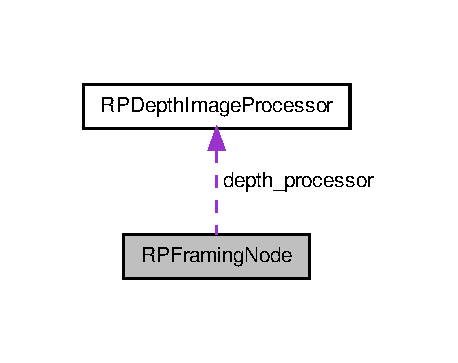
\includegraphics[width=220pt]{class_r_p_framing_node__coll__graph}
\end{center}
\end{figure}
\subsection*{\-Classes}
\begin{DoxyCompactItemize}
\item 
struct \hyperlink{struct_r_p_framing_node_1_1_r_p_rectangle_comparator}{\-R\-P\-Rectangle\-Comparator}
\end{DoxyCompactItemize}
\subsection*{\-Public \-Member \-Functions}
\begin{DoxyCompactItemize}
\item 
\hyperlink{class_r_p_framing_node_a673807f4faa477371ed702853867d696}{\-R\-P\-Framing\-Node} (ros\-::\-Node\-Handle \&\hyperlink{class_r_p_framing_node_ada7424816ecc44a22fc3f96eb32ed51d}{node})
\end{DoxyCompactItemize}
\subsection*{\-Private \-Member \-Functions}
\begin{DoxyCompactItemize}
\item 
void \hyperlink{class_r_p_framing_node_a0382670cfd83cd3002623e8969907ea7}{head\-Tracker\-Message\-Callback} (const rp\-\_\-head\-\_\-tracking\-::\-Heads \&tracked\-\_\-heads)
\item 
void \hyperlink{class_r_p_framing_node_a296105b2c174c8d616d6d05d889f22f9}{depth\-Image\-Callback} (const sensor\-\_\-msgs\-::\-Image\-::\-Const\-Ptr \&depth\-\_\-input\-\_\-image)
\item 
void \hyperlink{class_r_p_framing_node_ac5324e2882cac58d1bae6b82eb08a145}{initialize\-Rotation\-Vector} ()
\item 
void \hyperlink{class_r_p_framing_node_aa53b691c9287fc4435fc0ec4d3ac0127}{initialize\-Translation\-Vector} ()
\item 
void \hyperlink{class_r_p_framing_node_a8309f74244cb885c2538a33b10cc518d}{convert\-To\-Kinect\-Camera\-Coordinates} (const rp\-\_\-head\-\_\-tracking\-::\-Heads \&tracked\-\_\-heads, std\-::vector$<$ cv\-::\-Point3f $>$ \&projected\-\_\-points)
\item 
void \hyperlink{class_r_p_framing_node_a6d5f20f9074b914f657a038cd325272d}{convert\-To\-Camera\-Image\-Coordinates} (const std\-::vector$<$ cv\-::\-Point3f $>$ \&head\-\_\-points, std\-::vector$<$ cv\-::\-Rect $>$ \&projected\-\_\-head\-\_\-rectangles)
\item 
int \hyperlink{class_r_p_framing_node_aa2db07c46763d4b9e00ef82d56a11c5b}{centermost\-Head\-Rectangle\-Index} (const std\-::vector$<$ cv\-::\-Rect $>$ \&head\-\_\-rectangles)
\item 
void \hyperlink{class_r_p_framing_node_a978fc35a57bcab9aa873756d27a6c54a}{get\-Candidates\-In\-Frame} (const std\-::vector$<$ cv\-::\-Rect $>$ \&candidate\-\_\-head\-\_\-rectangles, const cv\-::\-Rect \&\hyperlink{class_r_p_framing_node_a1e4cba34d01b81db86ae54435d98ec76}{frame}, std\-::set$<$ cv\-::\-Rect, \hyperlink{struct_r_p_framing_node_1_1_r_p_rectangle_comparator}{\-R\-P\-Rectangle\-Comparator} $>$ \&candidates\-\_\-in\-\_\-frame)
\item 
void \hyperlink{class_r_p_framing_node_a7d7448265127cd1082f124a2bbd7e7e7}{frame\-Single\-Person} (const cv\-::\-Rect \&head\-\_\-rectangle, bool off\-\_\-center\-\_\-left, cv\-::\-Rect \&\hyperlink{class_r_p_framing_node_a1e4cba34d01b81db86ae54435d98ec76}{frame})
\item 
void \hyperlink{class_r_p_framing_node_af30fa6293069c2f2748702920c92c885}{frame\-Wide\-Group} (const cv\-::\-Rect \&bounding\-\_\-rectangle, cv\-::\-Rect \&\hyperlink{class_r_p_framing_node_a1e4cba34d01b81db86ae54435d98ec76}{frame})
\item 
void \hyperlink{class_r_p_framing_node_a0f8ddf2c1893f4bcc36414948a179a83}{frame\-Narrow\-Group} (const cv\-::\-Rect \&bounding\-\_\-rectangle, cv\-::\-Rect \&\hyperlink{class_r_p_framing_node_a1e4cba34d01b81db86ae54435d98ec76}{frame})
\item 
void \hyperlink{class_r_p_framing_node_a77640fd8d50fd4b075e8ef3be2e8e7bd}{publish\-Framing\-Status} (const std\-::vector$<$ cv\-::\-Rect $>$ $\ast$head\-\_\-rectangles)
\item 
void \hyperlink{class_r_p_framing_node_ae09715b4156667c15f5ca9123f77865a}{publish\-Driving\-Direction} ()
\item 
void \hyperlink{class_r_p_framing_node_aeb153d1d84d2698669375139b9277ead}{refresh\-Node\-Enabled\-Status} ()
\item 
void \hyperlink{class_r_p_framing_node_a666e1534a89c6096a5539f95efc49dd1}{get\-Overridable\-Parameters} ()
\end{DoxyCompactItemize}
\subsection*{\-Private \-Attributes}
\begin{DoxyCompactItemize}
\item 
ros\-::\-Node\-Handle \& \hyperlink{class_r_p_framing_node_ada7424816ecc44a22fc3f96eb32ed51d}{node}
\item 
bool \hyperlink{class_r_p_framing_node_a59242d677df9d2ef09ac222c98203a2d}{node\-\_\-enabled}
\item 
ros\-::\-Wall\-Time \hyperlink{class_r_p_framing_node_ac14e461ed967dd726303ff86c7f065e2}{enable\-\_\-time}
\item 
\-Framing\-Status \hyperlink{class_r_p_framing_node_adcfd6823bc9579a1deb6ca6640f44b93}{framing\-\_\-status}
\item 
cv\-::\-Rect \hyperlink{class_r_p_framing_node_a1e4cba34d01b81db86ae54435d98ec76}{frame}
\item 
\-Driving\-Direction \hyperlink{class_r_p_framing_node_a6a5e5171d0d882e21e9caee5977917ed}{driving\-\_\-direction}
\item 
ros\-::\-Publisher \hyperlink{class_r_p_framing_node_a790bcf735ba2a573f27be72ad2c0f1b3}{driving\-\_\-direction\-\_\-publisher}
\item 
ros\-::\-Publisher \hyperlink{class_r_p_framing_node_ae72d8d6735b444261bcb202f928404cc}{frame\-\_\-publisher}
\item 
ros\-::\-Subscriber \hyperlink{class_r_p_framing_node_ae1c216c2215db5cebcf18e1f7a51ae3f}{head\-\_\-tracker\-\_\-subscriber}
\item 
const cv\-::\-Rect \hyperlink{class_r_p_framing_node_a6773f17e9534cc005d5a3f2b749e3e72}{\-C\-A\-M\-E\-R\-A\-\_\-\-F\-R\-A\-M\-E\-\_\-\-R\-E\-C\-T\-A\-N\-G\-L\-E}
\item 
ros\-::\-Subscriber \hyperlink{class_r_p_framing_node_af473bf98f3e2f4653e5aaaec8a11a726}{depth\-\_\-subscriber}
\item 
\hyperlink{class_r_p_depth_image_processor}{\-R\-P\-Depth\-Image\-Processor} \hyperlink{class_r_p_framing_node_a40add69b2b615d2293c8c100606146b6}{depth\-\_\-processor}
\item 
ros\-::\-Service\-Client \hyperlink{class_r_p_framing_node_aedaa9ec0ee3cf711f893fbe242ebc5a8}{camera\-\_\-client}
\item 
cv\-::\-Mat \hyperlink{class_r_p_framing_node_a4a7d5d460e11aece880b5e9836d149dc}{camera\-\_\-matrix}
\item 
cv\-::\-Mat \hyperlink{class_r_p_framing_node_a312c193fe5662a8062a4f6d0918962f8}{distortion\-\_\-coefficients}
\item 
cv\-::\-Mat \hyperlink{class_r_p_framing_node_a118f00fa5a583971493536d0374a1a80}{rotation\-\_\-vector}
\item 
cv\-::\-Mat \hyperlink{class_r_p_framing_node_a69f636be3f1cc2793e48596a1da71909}{translation\-\_\-vector}
\item 
const std\-::string \hyperlink{class_r_p_framing_node_a144c66f7dcab4a463222f44d48128a5d}{\-W\-I\-N\-D\-O\-W\-\_\-\-N\-A\-M\-E}
\item 
double \hyperlink{class_r_p_framing_node_a583866e6d7361f07a7fdd5e0d357b251}{\-C\-A\-M\-E\-R\-A\-\_\-\-T\-R\-A\-N\-S\-L\-A\-T\-I\-O\-N\-\_\-\-X}
\item 
double \hyperlink{class_r_p_framing_node_a64ee86907af0fccc401e72fcbfac8df4}{\-C\-A\-M\-E\-R\-A\-\_\-\-T\-R\-A\-N\-S\-L\-A\-T\-I\-O\-N\-\_\-\-Y}
\item 
double \hyperlink{class_r_p_framing_node_a6b93f87ce0907cf58a5d24456ab9ccb4}{\-C\-A\-M\-E\-R\-A\-\_\-\-T\-R\-A\-N\-S\-L\-A\-T\-I\-O\-N\-\_\-\-Z}
\item 
double \hyperlink{class_r_p_framing_node_a66f21072e0ca3190decc590933a83cdb}{\-C\-A\-M\-E\-R\-A\-\_\-\-R\-O\-T\-A\-T\-I\-O\-N\-\_\-\-X}
\item 
double \hyperlink{class_r_p_framing_node_a9aad5136e8873e8b15012db9e2b56ec6}{\-C\-A\-M\-E\-R\-A\-\_\-\-R\-O\-T\-A\-T\-I\-O\-N\-\_\-\-Y}
\item 
double \hyperlink{class_r_p_framing_node_a2f7f848008e9c555f17fc418c65c0fb1}{\-C\-A\-M\-E\-R\-A\-\_\-\-R\-O\-T\-A\-T\-I\-O\-N\-\_\-\-Z}
\item 
bool \hyperlink{class_r_p_framing_node_a8c5a4411117ae10fe4ff69c0fa3fb465}{\-G\-U\-I\-\_\-\-O\-U\-T\-P\-U\-T\-\_\-\-E\-N\-A\-B\-L\-E\-D}
\end{DoxyCompactItemize}


\subsection{\-Detailed \-Description}
\-Robot photographer's photographic composition node, which uses the human head locations provided by the head tracking node to calculate the most aesthetically pleasing framing for the picture. 

\begin{DoxyCopyright}{\-Copyright}
\-Manfredas \-Zabarauskas, 2013. \-All rights reserved. \-This project is released under \-C\-C \-B\-Y-\/\-N\-C-\/\-S\-A (\-Creative \-Commons \-Attribution-\/\-Non\-Commercial-\/\-Share\-Alike) license. 
\end{DoxyCopyright}


\-Definition at line 70 of file framing.\-hpp.



\subsection{\-Constructor \& \-Destructor \-Documentation}
\hypertarget{class_r_p_framing_node_a673807f4faa477371ed702853867d696}{\index{\-R\-P\-Framing\-Node@{\-R\-P\-Framing\-Node}!\-R\-P\-Framing\-Node@{\-R\-P\-Framing\-Node}}
\index{\-R\-P\-Framing\-Node@{\-R\-P\-Framing\-Node}!RPFramingNode@{\-R\-P\-Framing\-Node}}
\subsubsection[{\-R\-P\-Framing\-Node}]{\setlength{\rightskip}{0pt plus 5cm}{\bf \-R\-P\-Framing\-Node\-::\-R\-P\-Framing\-Node} (
\begin{DoxyParamCaption}
\item[{ros\-::\-Node\-Handle \&}]{node}
\end{DoxyParamCaption}
)}}\label{class_r_p_framing_node_a673807f4faa477371ed702853867d696}
\-Default composition and framing node's constructor. 
\begin{DoxyParams}{\-Parameters}
{\em node} & \-Handle to \-R\-O\-S node. \\
\hline
\end{DoxyParams}


\-Definition at line 39 of file framing.\-cpp.



\subsection{\-Member \-Function \-Documentation}
\hypertarget{class_r_p_framing_node_aa2db07c46763d4b9e00ef82d56a11c5b}{\index{\-R\-P\-Framing\-Node@{\-R\-P\-Framing\-Node}!centermost\-Head\-Rectangle\-Index@{centermost\-Head\-Rectangle\-Index}}
\index{centermost\-Head\-Rectangle\-Index@{centermost\-Head\-Rectangle\-Index}!RPFramingNode@{\-R\-P\-Framing\-Node}}
\subsubsection[{centermost\-Head\-Rectangle\-Index}]{\setlength{\rightskip}{0pt plus 5cm}int {\bf \-R\-P\-Framing\-Node\-::centermost\-Head\-Rectangle\-Index} (
\begin{DoxyParamCaption}
\item[{const std\-::vector$<$ cv\-::\-Rect $>$ \&}]{head\-\_\-rectangles}
\end{DoxyParamCaption}
)\hspace{0.3cm}{\ttfamily  \mbox{[}private\mbox{]}}}}\label{class_r_p_framing_node_aa2db07c46763d4b9e00ef82d56a11c5b}
\-Finds the index of the rectangle closest to the camera frame center. 
\begin{DoxyParams}{\-Parameters}
{\em head\-\_\-rectangles} & \-Detected head rectangles. \\
\hline
\end{DoxyParams}


\-Definition at line 537 of file framing.\-cpp.

\hypertarget{class_r_p_framing_node_a6d5f20f9074b914f657a038cd325272d}{\index{\-R\-P\-Framing\-Node@{\-R\-P\-Framing\-Node}!convert\-To\-Camera\-Image\-Coordinates@{convert\-To\-Camera\-Image\-Coordinates}}
\index{convert\-To\-Camera\-Image\-Coordinates@{convert\-To\-Camera\-Image\-Coordinates}!RPFramingNode@{\-R\-P\-Framing\-Node}}
\subsubsection[{convert\-To\-Camera\-Image\-Coordinates}]{\setlength{\rightskip}{0pt plus 5cm}void {\bf \-R\-P\-Framing\-Node\-::convert\-To\-Camera\-Image\-Coordinates} (
\begin{DoxyParamCaption}
\item[{const std\-::vector$<$ cv\-::\-Point3f $>$ \&}]{head\-\_\-points, }
\item[{std\-::vector$<$ cv\-::\-Rect $>$ \&}]{projected\-\_\-head\-\_\-rectangles}
\end{DoxyParamCaption}
)\hspace{0.3cm}{\ttfamily  \mbox{[}private\mbox{]}}}}\label{class_r_p_framing_node_a6d5f20f9074b914f657a038cd325272d}
\-Converts top-\/left/bottom-\/right head rectangle points in the \-Kinect camera coordinates to head rectangles in the photographic camera's image plane. 
\begin{DoxyParams}{\-Parameters}
{\em head\-\_\-points} & 3\-D top-\/left/bottom-\/right head rectangle points in \-Kinect's coordinate system. \\
\hline
{\em projected\-\_\-head\-\_\-rectangles} & \-Projected head rectangles in the photographic camera's image plane. \\
\hline
\end{DoxyParams}


\-Definition at line 561 of file framing.\-cpp.

\hypertarget{class_r_p_framing_node_a8309f74244cb885c2538a33b10cc518d}{\index{\-R\-P\-Framing\-Node@{\-R\-P\-Framing\-Node}!convert\-To\-Kinect\-Camera\-Coordinates@{convert\-To\-Kinect\-Camera\-Coordinates}}
\index{convert\-To\-Kinect\-Camera\-Coordinates@{convert\-To\-Kinect\-Camera\-Coordinates}!RPFramingNode@{\-R\-P\-Framing\-Node}}
\subsubsection[{convert\-To\-Kinect\-Camera\-Coordinates}]{\setlength{\rightskip}{0pt plus 5cm}void {\bf \-R\-P\-Framing\-Node\-::convert\-To\-Kinect\-Camera\-Coordinates} (
\begin{DoxyParamCaption}
\item[{const rp\-\_\-head\-\_\-tracking\-::\-Heads \&}]{tracked\-\_\-heads, }
\item[{std\-::vector$<$ cv\-::\-Point3f $>$ \&}]{projected\-\_\-points}
\end{DoxyParamCaption}
)\hspace{0.3cm}{\ttfamily  \mbox{[}private\mbox{]}}}}\label{class_r_p_framing_node_a8309f74244cb885c2538a33b10cc518d}
\-Converts tracked heads to top-\/left/bottom-\/right head rectangle points in the \-Kinect's camera coordinates. 
\begin{DoxyParams}{\-Parameters}
{\em tracked\-\_\-heads} & \-Tracked head rectangles in \-Kinect's image plane. \\
\hline
{\em projected\-\_\-points} & \-Projected top-\/left/bottom-\/right head rectangle points in \-Kinect's world coordinate system. \\
\hline
\end{DoxyParams}


\-Definition at line 583 of file framing.\-cpp.

\hypertarget{class_r_p_framing_node_a296105b2c174c8d616d6d05d889f22f9}{\index{\-R\-P\-Framing\-Node@{\-R\-P\-Framing\-Node}!depth\-Image\-Callback@{depth\-Image\-Callback}}
\index{depth\-Image\-Callback@{depth\-Image\-Callback}!RPFramingNode@{\-R\-P\-Framing\-Node}}
\subsubsection[{depth\-Image\-Callback}]{\setlength{\rightskip}{0pt plus 5cm}void {\bf \-R\-P\-Framing\-Node\-::depth\-Image\-Callback} (
\begin{DoxyParamCaption}
\item[{const sensor\-\_\-msgs\-::\-Image\-::\-Const\-Ptr \&}]{depth\-\_\-input\-\_\-image}
\end{DoxyParamCaption}
)\hspace{0.3cm}{\ttfamily  \mbox{[}private\mbox{]}}}}\label{class_r_p_framing_node_a296105b2c174c8d616d6d05d889f22f9}
\-Depth image callback. 
\begin{DoxyParams}{\-Parameters}
{\em depth\-\_\-input\-\_\-image} & \-Pointer to depth input image. \\
\hline
\end{DoxyParams}


\-Definition at line 167 of file framing.\-cpp.

\hypertarget{class_r_p_framing_node_a0f8ddf2c1893f4bcc36414948a179a83}{\index{\-R\-P\-Framing\-Node@{\-R\-P\-Framing\-Node}!frame\-Narrow\-Group@{frame\-Narrow\-Group}}
\index{frame\-Narrow\-Group@{frame\-Narrow\-Group}!RPFramingNode@{\-R\-P\-Framing\-Node}}
\subsubsection[{frame\-Narrow\-Group}]{\setlength{\rightskip}{0pt plus 5cm}void {\bf \-R\-P\-Framing\-Node\-::frame\-Narrow\-Group} (
\begin{DoxyParamCaption}
\item[{const cv\-::\-Rect \&}]{bounding\-\_\-rectangle, }
\item[{cv\-::\-Rect \&}]{frame}
\end{DoxyParamCaption}
)\hspace{0.3cm}{\ttfamily  \mbox{[}private\mbox{]}}}}\label{class_r_p_framing_node_a0f8ddf2c1893f4bcc36414948a179a83}
\-Calculates the best frame for a narrow group of heads. 
\begin{DoxyParams}{\-Parameters}
{\em bounding\-\_\-rectangle} & \-Bounding rectangle for a candidate set of heads. \\
\hline
{\em frame} & \-Resulting frame. \\
\hline
\end{DoxyParams}


\-Definition at line 503 of file framing.\-cpp.

\hypertarget{class_r_p_framing_node_a7d7448265127cd1082f124a2bbd7e7e7}{\index{\-R\-P\-Framing\-Node@{\-R\-P\-Framing\-Node}!frame\-Single\-Person@{frame\-Single\-Person}}
\index{frame\-Single\-Person@{frame\-Single\-Person}!RPFramingNode@{\-R\-P\-Framing\-Node}}
\subsubsection[{frame\-Single\-Person}]{\setlength{\rightskip}{0pt plus 5cm}void {\bf \-R\-P\-Framing\-Node\-::frame\-Single\-Person} (
\begin{DoxyParamCaption}
\item[{const cv\-::\-Rect \&}]{head\-\_\-rectangle, }
\item[{bool}]{off\-\_\-center\-\_\-left, }
\item[{cv\-::\-Rect \&}]{frame}
\end{DoxyParamCaption}
)\hspace{0.3cm}{\ttfamily  \mbox{[}private\mbox{]}}}}\label{class_r_p_framing_node_a7d7448265127cd1082f124a2bbd7e7e7}
\-Calculates the best frame for a single person. 
\begin{DoxyParams}{\-Parameters}
{\em head\-\_\-rectangle} & \hyperlink{struct_head}{\-Head} rectangle for a candidate head. \\
\hline
{\em off\-\_\-center\-\_\-left} & \-Flag describing whether the face should be slightly off-\/centered to the left or to the right. \\
\hline
{\em frame} & \-Resulting frame. \\
\hline
\end{DoxyParams}


\-Definition at line 518 of file framing.\-cpp.

\hypertarget{class_r_p_framing_node_af30fa6293069c2f2748702920c92c885}{\index{\-R\-P\-Framing\-Node@{\-R\-P\-Framing\-Node}!frame\-Wide\-Group@{frame\-Wide\-Group}}
\index{frame\-Wide\-Group@{frame\-Wide\-Group}!RPFramingNode@{\-R\-P\-Framing\-Node}}
\subsubsection[{frame\-Wide\-Group}]{\setlength{\rightskip}{0pt plus 5cm}void {\bf \-R\-P\-Framing\-Node\-::frame\-Wide\-Group} (
\begin{DoxyParamCaption}
\item[{const cv\-::\-Rect \&}]{bounding\-\_\-rectangle, }
\item[{cv\-::\-Rect \&}]{frame}
\end{DoxyParamCaption}
)\hspace{0.3cm}{\ttfamily  \mbox{[}private\mbox{]}}}}\label{class_r_p_framing_node_af30fa6293069c2f2748702920c92c885}
\-Calculates the best frame for a wide group of heads. 
\begin{DoxyParams}{\-Parameters}
{\em bounding\-\_\-rectangle} & \-Bounding rectangle for a candidate set of heads. \\
\hline
{\em frame} & \-Resulting frame. \\
\hline
\end{DoxyParams}


\-Definition at line 487 of file framing.\-cpp.

\hypertarget{class_r_p_framing_node_a978fc35a57bcab9aa873756d27a6c54a}{\index{\-R\-P\-Framing\-Node@{\-R\-P\-Framing\-Node}!get\-Candidates\-In\-Frame@{get\-Candidates\-In\-Frame}}
\index{get\-Candidates\-In\-Frame@{get\-Candidates\-In\-Frame}!RPFramingNode@{\-R\-P\-Framing\-Node}}
\subsubsection[{get\-Candidates\-In\-Frame}]{\setlength{\rightskip}{0pt plus 5cm}void {\bf \-R\-P\-Framing\-Node\-::get\-Candidates\-In\-Frame} (
\begin{DoxyParamCaption}
\item[{const std\-::vector$<$ cv\-::\-Rect $>$ \&}]{candidate\-\_\-head\-\_\-rectangles, }
\item[{const cv\-::\-Rect \&}]{frame, }
\item[{std\-::set$<$ cv\-::\-Rect, {\bf \-R\-P\-Rectangle\-Comparator} $>$ \&}]{candidates\-\_\-in\-\_\-frame}
\end{DoxyParamCaption}
)\hspace{0.3cm}{\ttfamily  \mbox{[}private\mbox{]}}}}\label{class_r_p_framing_node_a978fc35a57bcab9aa873756d27a6c54a}
\-Finds the candidates whose head rectangles at least partially intersect with a given frame. 
\begin{DoxyParams}{\-Parameters}
{\em candidate\-\_\-head\-\_\-rectangles} & \-Detected head rectangles. \\
\hline
{\em frame} & \-Current ideal frame. \\
\hline
{\em candidates\-\_\-in\-\_\-frame} & \-Resulting candidates in the frame. \\
\hline
\end{DoxyParams}


\-Definition at line 475 of file framing.\-cpp.

\hypertarget{class_r_p_framing_node_a666e1534a89c6096a5539f95efc49dd1}{\index{\-R\-P\-Framing\-Node@{\-R\-P\-Framing\-Node}!get\-Overridable\-Parameters@{get\-Overridable\-Parameters}}
\index{get\-Overridable\-Parameters@{get\-Overridable\-Parameters}!RPFramingNode@{\-R\-P\-Framing\-Node}}
\subsubsection[{get\-Overridable\-Parameters}]{\setlength{\rightskip}{0pt plus 5cm}void {\bf \-R\-P\-Framing\-Node\-::get\-Overridable\-Parameters} (
\begin{DoxyParamCaption}
{}
\end{DoxyParamCaption}
)\hspace{0.3cm}{\ttfamily  \mbox{[}private\mbox{]}}}}\label{class_r_p_framing_node_a666e1534a89c6096a5539f95efc49dd1}
\-Gets the overridable parameters from the parameter server. 

\-Definition at line 153 of file framing.\-cpp.

\hypertarget{class_r_p_framing_node_a0382670cfd83cd3002623e8969907ea7}{\index{\-R\-P\-Framing\-Node@{\-R\-P\-Framing\-Node}!head\-Tracker\-Message\-Callback@{head\-Tracker\-Message\-Callback}}
\index{head\-Tracker\-Message\-Callback@{head\-Tracker\-Message\-Callback}!RPFramingNode@{\-R\-P\-Framing\-Node}}
\subsubsection[{head\-Tracker\-Message\-Callback}]{\setlength{\rightskip}{0pt plus 5cm}void {\bf \-R\-P\-Framing\-Node\-::head\-Tracker\-Message\-Callback} (
\begin{DoxyParamCaption}
\item[{const rp\-\_\-head\-\_\-tracking\-::\-Heads \&}]{tracked\-\_\-heads}
\end{DoxyParamCaption}
)\hspace{0.3cm}{\ttfamily  \mbox{[}private\mbox{]}}}}\label{class_r_p_framing_node_a0382670cfd83cd3002623e8969907ea7}
\-Head-\/tracker callback. 
\begin{DoxyParams}{\-Parameters}
{\em tracked\-\_\-heads} & \-Message containing detected/tracked heads. \\
\hline
\end{DoxyParams}


\-Definition at line 258 of file framing.\-cpp.

\hypertarget{class_r_p_framing_node_ac5324e2882cac58d1bae6b82eb08a145}{\index{\-R\-P\-Framing\-Node@{\-R\-P\-Framing\-Node}!initialize\-Rotation\-Vector@{initialize\-Rotation\-Vector}}
\index{initialize\-Rotation\-Vector@{initialize\-Rotation\-Vector}!RPFramingNode@{\-R\-P\-Framing\-Node}}
\subsubsection[{initialize\-Rotation\-Vector}]{\setlength{\rightskip}{0pt plus 5cm}void {\bf \-R\-P\-Framing\-Node\-::initialize\-Rotation\-Vector} (
\begin{DoxyParamCaption}
{}
\end{DoxyParamCaption}
)\hspace{0.3cm}{\ttfamily  \mbox{[}private\mbox{]}}}}\label{class_r_p_framing_node_ac5324e2882cac58d1bae6b82eb08a145}
\-Initializes rotation vector as set by the overridable parameters (in \-Rodrigues representation). 

\-Definition at line 117 of file framing.\-cpp.

\hypertarget{class_r_p_framing_node_aa53b691c9287fc4435fc0ec4d3ac0127}{\index{\-R\-P\-Framing\-Node@{\-R\-P\-Framing\-Node}!initialize\-Translation\-Vector@{initialize\-Translation\-Vector}}
\index{initialize\-Translation\-Vector@{initialize\-Translation\-Vector}!RPFramingNode@{\-R\-P\-Framing\-Node}}
\subsubsection[{initialize\-Translation\-Vector}]{\setlength{\rightskip}{0pt plus 5cm}void {\bf \-R\-P\-Framing\-Node\-::initialize\-Translation\-Vector} (
\begin{DoxyParamCaption}
{}
\end{DoxyParamCaption}
)\hspace{0.3cm}{\ttfamily  \mbox{[}private\mbox{]}}}}\label{class_r_p_framing_node_aa53b691c9287fc4435fc0ec4d3ac0127}
\-Initializes translation vector as set by the overridable parameters. 

\-Definition at line 146 of file framing.\-cpp.

\hypertarget{class_r_p_framing_node_ae09715b4156667c15f5ca9123f77865a}{\index{\-R\-P\-Framing\-Node@{\-R\-P\-Framing\-Node}!publish\-Driving\-Direction@{publish\-Driving\-Direction}}
\index{publish\-Driving\-Direction@{publish\-Driving\-Direction}!RPFramingNode@{\-R\-P\-Framing\-Node}}
\subsubsection[{publish\-Driving\-Direction}]{\setlength{\rightskip}{0pt plus 5cm}void {\bf \-R\-P\-Framing\-Node\-::publish\-Driving\-Direction} (
\begin{DoxyParamCaption}
{}
\end{DoxyParamCaption}
)\hspace{0.3cm}{\ttfamily  \mbox{[}private\mbox{]}}}}\label{class_r_p_framing_node_ae09715b4156667c15f5ca9123f77865a}
\-Publishes the stored driving direction. 

\-Definition at line 440 of file framing.\-cpp.

\hypertarget{class_r_p_framing_node_a77640fd8d50fd4b075e8ef3be2e8e7bd}{\index{\-R\-P\-Framing\-Node@{\-R\-P\-Framing\-Node}!publish\-Framing\-Status@{publish\-Framing\-Status}}
\index{publish\-Framing\-Status@{publish\-Framing\-Status}!RPFramingNode@{\-R\-P\-Framing\-Node}}
\subsubsection[{publish\-Framing\-Status}]{\setlength{\rightskip}{0pt plus 5cm}void {\bf \-R\-P\-Framing\-Node\-::publish\-Framing\-Status} (
\begin{DoxyParamCaption}
\item[{const std\-::vector$<$ cv\-::\-Rect $>$ $\ast$}]{head\-\_\-rectangles}
\end{DoxyParamCaption}
)\hspace{0.3cm}{\ttfamily  \mbox{[}private\mbox{]}}}}\label{class_r_p_framing_node_a77640fd8d50fd4b075e8ef3be2e8e7bd}
\-Publishes the framing status including the ideal frame and the detected head rectangles in the photographic camera's image plane. 
\begin{DoxyParams}{\-Parameters}
{\em head\-\_\-rectangles} & \-Detected head rectangles reprojected into the photographic camera's image plane. \\
\hline
\end{DoxyParams}


\-Definition at line 449 of file framing.\-cpp.

\hypertarget{class_r_p_framing_node_aeb153d1d84d2698669375139b9277ead}{\index{\-R\-P\-Framing\-Node@{\-R\-P\-Framing\-Node}!refresh\-Node\-Enabled\-Status@{refresh\-Node\-Enabled\-Status}}
\index{refresh\-Node\-Enabled\-Status@{refresh\-Node\-Enabled\-Status}!RPFramingNode@{\-R\-P\-Framing\-Node}}
\subsubsection[{refresh\-Node\-Enabled\-Status}]{\setlength{\rightskip}{0pt plus 5cm}void {\bf \-R\-P\-Framing\-Node\-::refresh\-Node\-Enabled\-Status} (
\begin{DoxyParamCaption}
{}
\end{DoxyParamCaption}
)\hspace{0.3cm}{\ttfamily  \mbox{[}private\mbox{]}}}}\label{class_r_p_framing_node_aeb153d1d84d2698669375139b9277ead}
\-Retrieves the \char`\"{}node enabled\char`\"{} status from the parameter server and marks the time of the \char`\"{}enable the node\char`\"{} command issue. 

\-Definition at line 238 of file framing.\-cpp.



\subsection{\-Member \-Data \-Documentation}
\hypertarget{class_r_p_framing_node_aedaa9ec0ee3cf711f893fbe242ebc5a8}{\index{\-R\-P\-Framing\-Node@{\-R\-P\-Framing\-Node}!camera\-\_\-client@{camera\-\_\-client}}
\index{camera\-\_\-client@{camera\-\_\-client}!RPFramingNode@{\-R\-P\-Framing\-Node}}
\subsubsection[{camera\-\_\-client}]{\setlength{\rightskip}{0pt plus 5cm}ros\-::\-Service\-Client {\bf \-R\-P\-Framing\-Node\-::camera\-\_\-client}\hspace{0.3cm}{\ttfamily  \mbox{[}private\mbox{]}}}}\label{class_r_p_framing_node_aedaa9ec0ee3cf711f893fbe242ebc5a8}
\-Camera client (for debugging). 

\-Definition at line 111 of file framing.\-hpp.

\hypertarget{class_r_p_framing_node_a6773f17e9534cc005d5a3f2b749e3e72}{\index{\-R\-P\-Framing\-Node@{\-R\-P\-Framing\-Node}!\-C\-A\-M\-E\-R\-A\-\_\-\-F\-R\-A\-M\-E\-\_\-\-R\-E\-C\-T\-A\-N\-G\-L\-E@{\-C\-A\-M\-E\-R\-A\-\_\-\-F\-R\-A\-M\-E\-\_\-\-R\-E\-C\-T\-A\-N\-G\-L\-E}}
\index{\-C\-A\-M\-E\-R\-A\-\_\-\-F\-R\-A\-M\-E\-\_\-\-R\-E\-C\-T\-A\-N\-G\-L\-E@{\-C\-A\-M\-E\-R\-A\-\_\-\-F\-R\-A\-M\-E\-\_\-\-R\-E\-C\-T\-A\-N\-G\-L\-E}!RPFramingNode@{\-R\-P\-Framing\-Node}}
\subsubsection[{\-C\-A\-M\-E\-R\-A\-\_\-\-F\-R\-A\-M\-E\-\_\-\-R\-E\-C\-T\-A\-N\-G\-L\-E}]{\setlength{\rightskip}{0pt plus 5cm}const cv\-::\-Rect {\bf \-R\-P\-Framing\-Node\-::\-C\-A\-M\-E\-R\-A\-\_\-\-F\-R\-A\-M\-E\-\_\-\-R\-E\-C\-T\-A\-N\-G\-L\-E}\hspace{0.3cm}{\ttfamily  \mbox{[}private\mbox{]}}}}\label{class_r_p_framing_node_a6773f17e9534cc005d5a3f2b749e3e72}
\-Camera's frame rectangle. 

\-Definition at line 102 of file framing.\-hpp.

\hypertarget{class_r_p_framing_node_a4a7d5d460e11aece880b5e9836d149dc}{\index{\-R\-P\-Framing\-Node@{\-R\-P\-Framing\-Node}!camera\-\_\-matrix@{camera\-\_\-matrix}}
\index{camera\-\_\-matrix@{camera\-\_\-matrix}!RPFramingNode@{\-R\-P\-Framing\-Node}}
\subsubsection[{camera\-\_\-matrix}]{\setlength{\rightskip}{0pt plus 5cm}cv\-::\-Mat {\bf \-R\-P\-Framing\-Node\-::camera\-\_\-matrix}\hspace{0.3cm}{\ttfamily  \mbox{[}private\mbox{]}}}}\label{class_r_p_framing_node_a4a7d5d460e11aece880b5e9836d149dc}
\-Camera intrinsics matrix (for debugging). 

\-Definition at line 113 of file framing.\-hpp.

\hypertarget{class_r_p_framing_node_a66f21072e0ca3190decc590933a83cdb}{\index{\-R\-P\-Framing\-Node@{\-R\-P\-Framing\-Node}!\-C\-A\-M\-E\-R\-A\-\_\-\-R\-O\-T\-A\-T\-I\-O\-N\-\_\-\-X@{\-C\-A\-M\-E\-R\-A\-\_\-\-R\-O\-T\-A\-T\-I\-O\-N\-\_\-\-X}}
\index{\-C\-A\-M\-E\-R\-A\-\_\-\-R\-O\-T\-A\-T\-I\-O\-N\-\_\-\-X@{\-C\-A\-M\-E\-R\-A\-\_\-\-R\-O\-T\-A\-T\-I\-O\-N\-\_\-\-X}!RPFramingNode@{\-R\-P\-Framing\-Node}}
\subsubsection[{\-C\-A\-M\-E\-R\-A\-\_\-\-R\-O\-T\-A\-T\-I\-O\-N\-\_\-\-X}]{\setlength{\rightskip}{0pt plus 5cm}double {\bf \-R\-P\-Framing\-Node\-::\-C\-A\-M\-E\-R\-A\-\_\-\-R\-O\-T\-A\-T\-I\-O\-N\-\_\-\-X}\hspace{0.3cm}{\ttfamily  \mbox{[}private\mbox{]}}}}\label{class_r_p_framing_node_a66f21072e0ca3190decc590933a83cdb}
\-Camera rotation around \-X axis \-O\-P. 

\-Definition at line 129 of file framing.\-hpp.

\hypertarget{class_r_p_framing_node_a9aad5136e8873e8b15012db9e2b56ec6}{\index{\-R\-P\-Framing\-Node@{\-R\-P\-Framing\-Node}!\-C\-A\-M\-E\-R\-A\-\_\-\-R\-O\-T\-A\-T\-I\-O\-N\-\_\-\-Y@{\-C\-A\-M\-E\-R\-A\-\_\-\-R\-O\-T\-A\-T\-I\-O\-N\-\_\-\-Y}}
\index{\-C\-A\-M\-E\-R\-A\-\_\-\-R\-O\-T\-A\-T\-I\-O\-N\-\_\-\-Y@{\-C\-A\-M\-E\-R\-A\-\_\-\-R\-O\-T\-A\-T\-I\-O\-N\-\_\-\-Y}!RPFramingNode@{\-R\-P\-Framing\-Node}}
\subsubsection[{\-C\-A\-M\-E\-R\-A\-\_\-\-R\-O\-T\-A\-T\-I\-O\-N\-\_\-\-Y}]{\setlength{\rightskip}{0pt plus 5cm}double {\bf \-R\-P\-Framing\-Node\-::\-C\-A\-M\-E\-R\-A\-\_\-\-R\-O\-T\-A\-T\-I\-O\-N\-\_\-\-Y}\hspace{0.3cm}{\ttfamily  \mbox{[}private\mbox{]}}}}\label{class_r_p_framing_node_a9aad5136e8873e8b15012db9e2b56ec6}
\-Camera rotation around \-Y axis \-O\-P. 

\-Definition at line 130 of file framing.\-hpp.

\hypertarget{class_r_p_framing_node_a2f7f848008e9c555f17fc418c65c0fb1}{\index{\-R\-P\-Framing\-Node@{\-R\-P\-Framing\-Node}!\-C\-A\-M\-E\-R\-A\-\_\-\-R\-O\-T\-A\-T\-I\-O\-N\-\_\-\-Z@{\-C\-A\-M\-E\-R\-A\-\_\-\-R\-O\-T\-A\-T\-I\-O\-N\-\_\-\-Z}}
\index{\-C\-A\-M\-E\-R\-A\-\_\-\-R\-O\-T\-A\-T\-I\-O\-N\-\_\-\-Z@{\-C\-A\-M\-E\-R\-A\-\_\-\-R\-O\-T\-A\-T\-I\-O\-N\-\_\-\-Z}!RPFramingNode@{\-R\-P\-Framing\-Node}}
\subsubsection[{\-C\-A\-M\-E\-R\-A\-\_\-\-R\-O\-T\-A\-T\-I\-O\-N\-\_\-\-Z}]{\setlength{\rightskip}{0pt plus 5cm}double {\bf \-R\-P\-Framing\-Node\-::\-C\-A\-M\-E\-R\-A\-\_\-\-R\-O\-T\-A\-T\-I\-O\-N\-\_\-\-Z}\hspace{0.3cm}{\ttfamily  \mbox{[}private\mbox{]}}}}\label{class_r_p_framing_node_a2f7f848008e9c555f17fc418c65c0fb1}
\-Camera rotation around \-Z axis \-O\-P. 

\-Definition at line 131 of file framing.\-hpp.

\hypertarget{class_r_p_framing_node_a583866e6d7361f07a7fdd5e0d357b251}{\index{\-R\-P\-Framing\-Node@{\-R\-P\-Framing\-Node}!\-C\-A\-M\-E\-R\-A\-\_\-\-T\-R\-A\-N\-S\-L\-A\-T\-I\-O\-N\-\_\-\-X@{\-C\-A\-M\-E\-R\-A\-\_\-\-T\-R\-A\-N\-S\-L\-A\-T\-I\-O\-N\-\_\-\-X}}
\index{\-C\-A\-M\-E\-R\-A\-\_\-\-T\-R\-A\-N\-S\-L\-A\-T\-I\-O\-N\-\_\-\-X@{\-C\-A\-M\-E\-R\-A\-\_\-\-T\-R\-A\-N\-S\-L\-A\-T\-I\-O\-N\-\_\-\-X}!RPFramingNode@{\-R\-P\-Framing\-Node}}
\subsubsection[{\-C\-A\-M\-E\-R\-A\-\_\-\-T\-R\-A\-N\-S\-L\-A\-T\-I\-O\-N\-\_\-\-X}]{\setlength{\rightskip}{0pt plus 5cm}double {\bf \-R\-P\-Framing\-Node\-::\-C\-A\-M\-E\-R\-A\-\_\-\-T\-R\-A\-N\-S\-L\-A\-T\-I\-O\-N\-\_\-\-X}\hspace{0.3cm}{\ttfamily  \mbox{[}private\mbox{]}}}}\label{class_r_p_framing_node_a583866e6d7361f07a7fdd5e0d357b251}
\-Camera translation in \-X direction \-O\-P. 

\-Definition at line 125 of file framing.\-hpp.

\hypertarget{class_r_p_framing_node_a64ee86907af0fccc401e72fcbfac8df4}{\index{\-R\-P\-Framing\-Node@{\-R\-P\-Framing\-Node}!\-C\-A\-M\-E\-R\-A\-\_\-\-T\-R\-A\-N\-S\-L\-A\-T\-I\-O\-N\-\_\-\-Y@{\-C\-A\-M\-E\-R\-A\-\_\-\-T\-R\-A\-N\-S\-L\-A\-T\-I\-O\-N\-\_\-\-Y}}
\index{\-C\-A\-M\-E\-R\-A\-\_\-\-T\-R\-A\-N\-S\-L\-A\-T\-I\-O\-N\-\_\-\-Y@{\-C\-A\-M\-E\-R\-A\-\_\-\-T\-R\-A\-N\-S\-L\-A\-T\-I\-O\-N\-\_\-\-Y}!RPFramingNode@{\-R\-P\-Framing\-Node}}
\subsubsection[{\-C\-A\-M\-E\-R\-A\-\_\-\-T\-R\-A\-N\-S\-L\-A\-T\-I\-O\-N\-\_\-\-Y}]{\setlength{\rightskip}{0pt plus 5cm}double {\bf \-R\-P\-Framing\-Node\-::\-C\-A\-M\-E\-R\-A\-\_\-\-T\-R\-A\-N\-S\-L\-A\-T\-I\-O\-N\-\_\-\-Y}\hspace{0.3cm}{\ttfamily  \mbox{[}private\mbox{]}}}}\label{class_r_p_framing_node_a64ee86907af0fccc401e72fcbfac8df4}
\-Camera translation in \-Y direction \-O\-P. 

\-Definition at line 126 of file framing.\-hpp.

\hypertarget{class_r_p_framing_node_a6b93f87ce0907cf58a5d24456ab9ccb4}{\index{\-R\-P\-Framing\-Node@{\-R\-P\-Framing\-Node}!\-C\-A\-M\-E\-R\-A\-\_\-\-T\-R\-A\-N\-S\-L\-A\-T\-I\-O\-N\-\_\-\-Z@{\-C\-A\-M\-E\-R\-A\-\_\-\-T\-R\-A\-N\-S\-L\-A\-T\-I\-O\-N\-\_\-\-Z}}
\index{\-C\-A\-M\-E\-R\-A\-\_\-\-T\-R\-A\-N\-S\-L\-A\-T\-I\-O\-N\-\_\-\-Z@{\-C\-A\-M\-E\-R\-A\-\_\-\-T\-R\-A\-N\-S\-L\-A\-T\-I\-O\-N\-\_\-\-Z}!RPFramingNode@{\-R\-P\-Framing\-Node}}
\subsubsection[{\-C\-A\-M\-E\-R\-A\-\_\-\-T\-R\-A\-N\-S\-L\-A\-T\-I\-O\-N\-\_\-\-Z}]{\setlength{\rightskip}{0pt plus 5cm}double {\bf \-R\-P\-Framing\-Node\-::\-C\-A\-M\-E\-R\-A\-\_\-\-T\-R\-A\-N\-S\-L\-A\-T\-I\-O\-N\-\_\-\-Z}\hspace{0.3cm}{\ttfamily  \mbox{[}private\mbox{]}}}}\label{class_r_p_framing_node_a6b93f87ce0907cf58a5d24456ab9ccb4}
\-Camera translation in \-Z direction \-O\-P. 

\-Definition at line 127 of file framing.\-hpp.

\hypertarget{class_r_p_framing_node_a40add69b2b615d2293c8c100606146b6}{\index{\-R\-P\-Framing\-Node@{\-R\-P\-Framing\-Node}!depth\-\_\-processor@{depth\-\_\-processor}}
\index{depth\-\_\-processor@{depth\-\_\-processor}!RPFramingNode@{\-R\-P\-Framing\-Node}}
\subsubsection[{depth\-\_\-processor}]{\setlength{\rightskip}{0pt plus 5cm}{\bf \-R\-P\-Depth\-Image\-Processor} {\bf \-R\-P\-Framing\-Node\-::depth\-\_\-processor}\hspace{0.3cm}{\ttfamily  \mbox{[}private\mbox{]}}}}\label{class_r_p_framing_node_a40add69b2b615d2293c8c100606146b6}
\-Kinect depth image processor (for debugging). 

\-Definition at line 108 of file framing.\-hpp.

\hypertarget{class_r_p_framing_node_af473bf98f3e2f4653e5aaaec8a11a726}{\index{\-R\-P\-Framing\-Node@{\-R\-P\-Framing\-Node}!depth\-\_\-subscriber@{depth\-\_\-subscriber}}
\index{depth\-\_\-subscriber@{depth\-\_\-subscriber}!RPFramingNode@{\-R\-P\-Framing\-Node}}
\subsubsection[{depth\-\_\-subscriber}]{\setlength{\rightskip}{0pt plus 5cm}ros\-::\-Subscriber {\bf \-R\-P\-Framing\-Node\-::depth\-\_\-subscriber}\hspace{0.3cm}{\ttfamily  \mbox{[}private\mbox{]}}}}\label{class_r_p_framing_node_af473bf98f3e2f4653e5aaaec8a11a726}
\-Kinect depth input subscriber (for debugging). 

\-Definition at line 105 of file framing.\-hpp.

\hypertarget{class_r_p_framing_node_a312c193fe5662a8062a4f6d0918962f8}{\index{\-R\-P\-Framing\-Node@{\-R\-P\-Framing\-Node}!distortion\-\_\-coefficients@{distortion\-\_\-coefficients}}
\index{distortion\-\_\-coefficients@{distortion\-\_\-coefficients}!RPFramingNode@{\-R\-P\-Framing\-Node}}
\subsubsection[{distortion\-\_\-coefficients}]{\setlength{\rightskip}{0pt plus 5cm}cv\-::\-Mat {\bf \-R\-P\-Framing\-Node\-::distortion\-\_\-coefficients}\hspace{0.3cm}{\ttfamily  \mbox{[}private\mbox{]}}}}\label{class_r_p_framing_node_a312c193fe5662a8062a4f6d0918962f8}
\-Camera distortion coefficients (for debugging). 

\-Definition at line 115 of file framing.\-hpp.

\hypertarget{class_r_p_framing_node_a6a5e5171d0d882e21e9caee5977917ed}{\index{\-R\-P\-Framing\-Node@{\-R\-P\-Framing\-Node}!driving\-\_\-direction@{driving\-\_\-direction}}
\index{driving\-\_\-direction@{driving\-\_\-direction}!RPFramingNode@{\-R\-P\-Framing\-Node}}
\subsubsection[{driving\-\_\-direction}]{\setlength{\rightskip}{0pt plus 5cm}\-Driving\-Direction {\bf \-R\-P\-Framing\-Node\-::driving\-\_\-direction}\hspace{0.3cm}{\ttfamily  \mbox{[}private\mbox{]}}}}\label{class_r_p_framing_node_a6a5e5171d0d882e21e9caee5977917ed}
\-Produced driving direction suggestion. 

\-Definition at line 95 of file framing.\-hpp.

\hypertarget{class_r_p_framing_node_a790bcf735ba2a573f27be72ad2c0f1b3}{\index{\-R\-P\-Framing\-Node@{\-R\-P\-Framing\-Node}!driving\-\_\-direction\-\_\-publisher@{driving\-\_\-direction\-\_\-publisher}}
\index{driving\-\_\-direction\-\_\-publisher@{driving\-\_\-direction\-\_\-publisher}!RPFramingNode@{\-R\-P\-Framing\-Node}}
\subsubsection[{driving\-\_\-direction\-\_\-publisher}]{\setlength{\rightskip}{0pt plus 5cm}ros\-::\-Publisher {\bf \-R\-P\-Framing\-Node\-::driving\-\_\-direction\-\_\-publisher}\hspace{0.3cm}{\ttfamily  \mbox{[}private\mbox{]}}}}\label{class_r_p_framing_node_a790bcf735ba2a573f27be72ad2c0f1b3}
\-Driving direction publisher. 

\-Definition at line 97 of file framing.\-hpp.

\hypertarget{class_r_p_framing_node_ac14e461ed967dd726303ff86c7f065e2}{\index{\-R\-P\-Framing\-Node@{\-R\-P\-Framing\-Node}!enable\-\_\-time@{enable\-\_\-time}}
\index{enable\-\_\-time@{enable\-\_\-time}!RPFramingNode@{\-R\-P\-Framing\-Node}}
\subsubsection[{enable\-\_\-time}]{\setlength{\rightskip}{0pt plus 5cm}ros\-::\-Wall\-Time {\bf \-R\-P\-Framing\-Node\-::enable\-\_\-time}\hspace{0.3cm}{\ttfamily  \mbox{[}private\mbox{]}}}}\label{class_r_p_framing_node_ac14e461ed967dd726303ff86c7f065e2}
\-Node's last enable time. 

\-Definition at line 90 of file framing.\-hpp.

\hypertarget{class_r_p_framing_node_a1e4cba34d01b81db86ae54435d98ec76}{\index{\-R\-P\-Framing\-Node@{\-R\-P\-Framing\-Node}!frame@{frame}}
\index{frame@{frame}!RPFramingNode@{\-R\-P\-Framing\-Node}}
\subsubsection[{frame}]{\setlength{\rightskip}{0pt plus 5cm}cv\-::\-Rect {\bf \-R\-P\-Framing\-Node\-::frame}\hspace{0.3cm}{\ttfamily  \mbox{[}private\mbox{]}}}}\label{class_r_p_framing_node_a1e4cba34d01b81db86ae54435d98ec76}
\-Produced ideal frame. 

\-Definition at line 94 of file framing.\-hpp.

\hypertarget{class_r_p_framing_node_ae72d8d6735b444261bcb202f928404cc}{\index{\-R\-P\-Framing\-Node@{\-R\-P\-Framing\-Node}!frame\-\_\-publisher@{frame\-\_\-publisher}}
\index{frame\-\_\-publisher@{frame\-\_\-publisher}!RPFramingNode@{\-R\-P\-Framing\-Node}}
\subsubsection[{frame\-\_\-publisher}]{\setlength{\rightskip}{0pt plus 5cm}ros\-::\-Publisher {\bf \-R\-P\-Framing\-Node\-::frame\-\_\-publisher}\hspace{0.3cm}{\ttfamily  \mbox{[}private\mbox{]}}}}\label{class_r_p_framing_node_ae72d8d6735b444261bcb202f928404cc}
\-Produced ideal frame publisher. 

\-Definition at line 98 of file framing.\-hpp.

\hypertarget{class_r_p_framing_node_adcfd6823bc9579a1deb6ca6640f44b93}{\index{\-R\-P\-Framing\-Node@{\-R\-P\-Framing\-Node}!framing\-\_\-status@{framing\-\_\-status}}
\index{framing\-\_\-status@{framing\-\_\-status}!RPFramingNode@{\-R\-P\-Framing\-Node}}
\subsubsection[{framing\-\_\-status}]{\setlength{\rightskip}{0pt plus 5cm}\-Framing\-Status {\bf \-R\-P\-Framing\-Node\-::framing\-\_\-status}\hspace{0.3cm}{\ttfamily  \mbox{[}private\mbox{]}}}}\label{class_r_p_framing_node_adcfd6823bc9579a1deb6ca6640f44b93}
\-Framing status. 

\-Definition at line 92 of file framing.\-hpp.

\hypertarget{class_r_p_framing_node_a8c5a4411117ae10fe4ff69c0fa3fb465}{\index{\-R\-P\-Framing\-Node@{\-R\-P\-Framing\-Node}!\-G\-U\-I\-\_\-\-O\-U\-T\-P\-U\-T\-\_\-\-E\-N\-A\-B\-L\-E\-D@{\-G\-U\-I\-\_\-\-O\-U\-T\-P\-U\-T\-\_\-\-E\-N\-A\-B\-L\-E\-D}}
\index{\-G\-U\-I\-\_\-\-O\-U\-T\-P\-U\-T\-\_\-\-E\-N\-A\-B\-L\-E\-D@{\-G\-U\-I\-\_\-\-O\-U\-T\-P\-U\-T\-\_\-\-E\-N\-A\-B\-L\-E\-D}!RPFramingNode@{\-R\-P\-Framing\-Node}}
\subsubsection[{\-G\-U\-I\-\_\-\-O\-U\-T\-P\-U\-T\-\_\-\-E\-N\-A\-B\-L\-E\-D}]{\setlength{\rightskip}{0pt plus 5cm}bool {\bf \-R\-P\-Framing\-Node\-::\-G\-U\-I\-\_\-\-O\-U\-T\-P\-U\-T\-\_\-\-E\-N\-A\-B\-L\-E\-D}\hspace{0.3cm}{\ttfamily  \mbox{[}private\mbox{]}}}}\label{class_r_p_framing_node_a8c5a4411117ae10fe4ff69c0fa3fb465}
\-G\-U\-I output enabled flag \-O\-P. 

\-Definition at line 133 of file framing.\-hpp.

\hypertarget{class_r_p_framing_node_ae1c216c2215db5cebcf18e1f7a51ae3f}{\index{\-R\-P\-Framing\-Node@{\-R\-P\-Framing\-Node}!head\-\_\-tracker\-\_\-subscriber@{head\-\_\-tracker\-\_\-subscriber}}
\index{head\-\_\-tracker\-\_\-subscriber@{head\-\_\-tracker\-\_\-subscriber}!RPFramingNode@{\-R\-P\-Framing\-Node}}
\subsubsection[{head\-\_\-tracker\-\_\-subscriber}]{\setlength{\rightskip}{0pt plus 5cm}ros\-::\-Subscriber {\bf \-R\-P\-Framing\-Node\-::head\-\_\-tracker\-\_\-subscriber}\hspace{0.3cm}{\ttfamily  \mbox{[}private\mbox{]}}}}\label{class_r_p_framing_node_ae1c216c2215db5cebcf18e1f7a51ae3f}
\-Head-\/tracking input subscriber. 

\-Definition at line 100 of file framing.\-hpp.

\hypertarget{class_r_p_framing_node_ada7424816ecc44a22fc3f96eb32ed51d}{\index{\-R\-P\-Framing\-Node@{\-R\-P\-Framing\-Node}!node@{node}}
\index{node@{node}!RPFramingNode@{\-R\-P\-Framing\-Node}}
\subsubsection[{node}]{\setlength{\rightskip}{0pt plus 5cm}ros\-::\-Node\-Handle\& {\bf \-R\-P\-Framing\-Node\-::node}\hspace{0.3cm}{\ttfamily  \mbox{[}private\mbox{]}}}}\label{class_r_p_framing_node_ada7424816ecc44a22fc3f96eb32ed51d}
\-Node's handle. 

\-Definition at line 87 of file framing.\-hpp.

\hypertarget{class_r_p_framing_node_a59242d677df9d2ef09ac222c98203a2d}{\index{\-R\-P\-Framing\-Node@{\-R\-P\-Framing\-Node}!node\-\_\-enabled@{node\-\_\-enabled}}
\index{node\-\_\-enabled@{node\-\_\-enabled}!RPFramingNode@{\-R\-P\-Framing\-Node}}
\subsubsection[{node\-\_\-enabled}]{\setlength{\rightskip}{0pt plus 5cm}bool {\bf \-R\-P\-Framing\-Node\-::node\-\_\-enabled}\hspace{0.3cm}{\ttfamily  \mbox{[}private\mbox{]}}}}\label{class_r_p_framing_node_a59242d677df9d2ef09ac222c98203a2d}
\-Node's enabled/disabled flag. 

\-Definition at line 88 of file framing.\-hpp.

\hypertarget{class_r_p_framing_node_a118f00fa5a583971493536d0374a1a80}{\index{\-R\-P\-Framing\-Node@{\-R\-P\-Framing\-Node}!rotation\-\_\-vector@{rotation\-\_\-vector}}
\index{rotation\-\_\-vector@{rotation\-\_\-vector}!RPFramingNode@{\-R\-P\-Framing\-Node}}
\subsubsection[{rotation\-\_\-vector}]{\setlength{\rightskip}{0pt plus 5cm}cv\-::\-Mat {\bf \-R\-P\-Framing\-Node\-::rotation\-\_\-vector}\hspace{0.3cm}{\ttfamily  \mbox{[}private\mbox{]}}}}\label{class_r_p_framing_node_a118f00fa5a583971493536d0374a1a80}
\-Camera rotation vector (w.\-r.\-t. robot's base; for debugging). 

\-Definition at line 117 of file framing.\-hpp.

\hypertarget{class_r_p_framing_node_a69f636be3f1cc2793e48596a1da71909}{\index{\-R\-P\-Framing\-Node@{\-R\-P\-Framing\-Node}!translation\-\_\-vector@{translation\-\_\-vector}}
\index{translation\-\_\-vector@{translation\-\_\-vector}!RPFramingNode@{\-R\-P\-Framing\-Node}}
\subsubsection[{translation\-\_\-vector}]{\setlength{\rightskip}{0pt plus 5cm}cv\-::\-Mat {\bf \-R\-P\-Framing\-Node\-::translation\-\_\-vector}\hspace{0.3cm}{\ttfamily  \mbox{[}private\mbox{]}}}}\label{class_r_p_framing_node_a69f636be3f1cc2793e48596a1da71909}
\-Camera translation vector (w.\-r.\-t. robot's base; for debugging). 

\-Definition at line 119 of file framing.\-hpp.

\hypertarget{class_r_p_framing_node_a144c66f7dcab4a463222f44d48128a5d}{\index{\-R\-P\-Framing\-Node@{\-R\-P\-Framing\-Node}!\-W\-I\-N\-D\-O\-W\-\_\-\-N\-A\-M\-E@{\-W\-I\-N\-D\-O\-W\-\_\-\-N\-A\-M\-E}}
\index{\-W\-I\-N\-D\-O\-W\-\_\-\-N\-A\-M\-E@{\-W\-I\-N\-D\-O\-W\-\_\-\-N\-A\-M\-E}!RPFramingNode@{\-R\-P\-Framing\-Node}}
\subsubsection[{\-W\-I\-N\-D\-O\-W\-\_\-\-N\-A\-M\-E}]{\setlength{\rightskip}{0pt plus 5cm}const std\-::string {\bf \-R\-P\-Framing\-Node\-::\-W\-I\-N\-D\-O\-W\-\_\-\-N\-A\-M\-E}\hspace{0.3cm}{\ttfamily  \mbox{[}private\mbox{]}}}}\label{class_r_p_framing_node_a144c66f7dcab4a463222f44d48128a5d}
\-Output window name (if \-G\-U\-I output is enabled). 

\-Definition at line 122 of file framing.\-hpp.



\-The documentation for this class was generated from the following files\-:\begin{DoxyCompactItemize}
\item 
rp\-\_\-framing/include/framing.\-hpp\item 
rp\-\_\-framing/src/framing.\-cpp\end{DoxyCompactItemize}

\hypertarget{class_r_p_heads_message_builder}{\section{\-R\-P\-Heads\-Message\-Builder \-Class \-Reference}
\label{class_r_p_heads_message_builder}\index{\-R\-P\-Heads\-Message\-Builder@{\-R\-P\-Heads\-Message\-Builder}}
}


\-Detected/tracked head message builder class.  




{\ttfamily \#include $<$heads\-\_\-message\-\_\-builder.\-hpp$>$}

\subsection*{\-Static \-Public \-Member \-Functions}
\begin{DoxyCompactItemize}
\item 
static void \hyperlink{class_r_p_heads_message_builder_a71fb699411567867dd4332b7fee22da4}{build\-Heads\-Message} (const std\-::string \&frame\-\_\-id, const unsigned int frame\-\_\-number, const ros\-::\-Time \&time\-\_\-stamp, const std\-::vector$<$ \hyperlink{struct_head}{\-Head} $>$ \&heads, const cv\-\_\-bridge\-::\-Cv\-Image\-::\-Const\-Ptr \&depth\-\_\-image, rp\-\_\-head\-\_\-tracking\-::\-Heads \&heads\-\_\-message)
\end{DoxyCompactItemize}


\subsection{\-Detailed \-Description}
\-Detected/tracked head message builder class. 

\begin{DoxyCopyright}{\-Copyright}
\-Manfredas \-Zabarauskas, 2013. \-All rights reserved. \-This project is released under \-C\-C \-B\-Y-\/\-N\-C-\/\-S\-A (\-Creative \-Commons \-Attribution-\/\-Non\-Commercial-\/\-Share\-Alike) license. 
\end{DoxyCopyright}


\-Definition at line 35 of file heads\-\_\-message\-\_\-builder.\-hpp.



\subsection{\-Member \-Function \-Documentation}
\hypertarget{class_r_p_heads_message_builder_a71fb699411567867dd4332b7fee22da4}{\index{\-R\-P\-Heads\-Message\-Builder@{\-R\-P\-Heads\-Message\-Builder}!build\-Heads\-Message@{build\-Heads\-Message}}
\index{build\-Heads\-Message@{build\-Heads\-Message}!RPHeadsMessageBuilder@{\-R\-P\-Heads\-Message\-Builder}}
\subsubsection[{build\-Heads\-Message}]{\setlength{\rightskip}{0pt plus 5cm}void {\bf \-R\-P\-Heads\-Message\-Builder\-::build\-Heads\-Message} (
\begin{DoxyParamCaption}
\item[{const std\-::string \&}]{frame\-\_\-id, }
\item[{const unsigned int}]{frame\-\_\-number, }
\item[{const ros\-::\-Time \&}]{time\-\_\-stamp, }
\item[{const std\-::vector$<$ {\bf \-Head} $>$ \&}]{heads, }
\item[{const cv\-\_\-bridge\-::\-Cv\-Image\-::\-Const\-Ptr \&}]{depth\-\_\-image, }
\item[{rp\-\_\-head\-\_\-tracking\-::\-Heads \&}]{heads\-\_\-message}
\end{DoxyParamCaption}
)\hspace{0.3cm}{\ttfamily  \mbox{[}static\mbox{]}}}}\label{class_r_p_heads_message_builder_a71fb699411567867dd4332b7fee22da4}
\-Builds a detected/tracked head message. 
\begin{DoxyParams}{\-Parameters}
{\em frame\-\_\-id} & \-Frame \-I\-D. \\
\hline
{\em frame\-\_\-number} & \-Current frame number. \\
\hline
{\em time\-\_\-stamp} & \-Current frame time stamp. \\
\hline
{\em heads} & \-Detected heads. \\
\hline
{\em depth\-\_\-image} & \-Depth image. \\
\hline
{\em heads\-\_\-message} & \-Built heads message.\\
\hline
\end{DoxyParams}
\begin{DoxyCopyright}{\-Copyright}
\-Manfredas \-Zabarauskas, 2013. \-All rights reserved. \-This project is released under \-C\-C \-B\-Y-\/\-N\-C-\/\-S\-A (\-Creative \-Commons \-Attribution-\/\-Non\-Commercial-\/\-Share\-Alike) license. 
\end{DoxyCopyright}


\-Definition at line 7 of file heads\-\_\-message\-\_\-builder.\-cpp.



\-The documentation for this class was generated from the following files\-:\begin{DoxyCompactItemize}
\item 
rp\-\_\-head\-\_\-tracking/include/heads\-\_\-message\-\_\-builder.\-hpp\item 
rp\-\_\-head\-\_\-tracking/src/heads\-\_\-message\-\_\-builder.\-cpp\end{DoxyCompactItemize}

\hypertarget{class_r_p_head_tracking_node}{\section{\-R\-P\-Head\-Tracking\-Node \-Class \-Reference}
\label{class_r_p_head_tracking_node}\index{\-R\-P\-Head\-Tracking\-Node@{\-R\-P\-Head\-Tracking\-Node}}
}


\-Robot photographer's head tracking node, which uses the colour and depth inputs from \-Kinect to detect and track humans in \-Luke's vicinity.  




{\ttfamily \#include $<$head\-\_\-tracking.\-hpp$>$}



\-Collaboration diagram for \-R\-P\-Head\-Tracking\-Node\-:\nopagebreak
\begin{figure}[H]
\begin{center}
\leavevmode
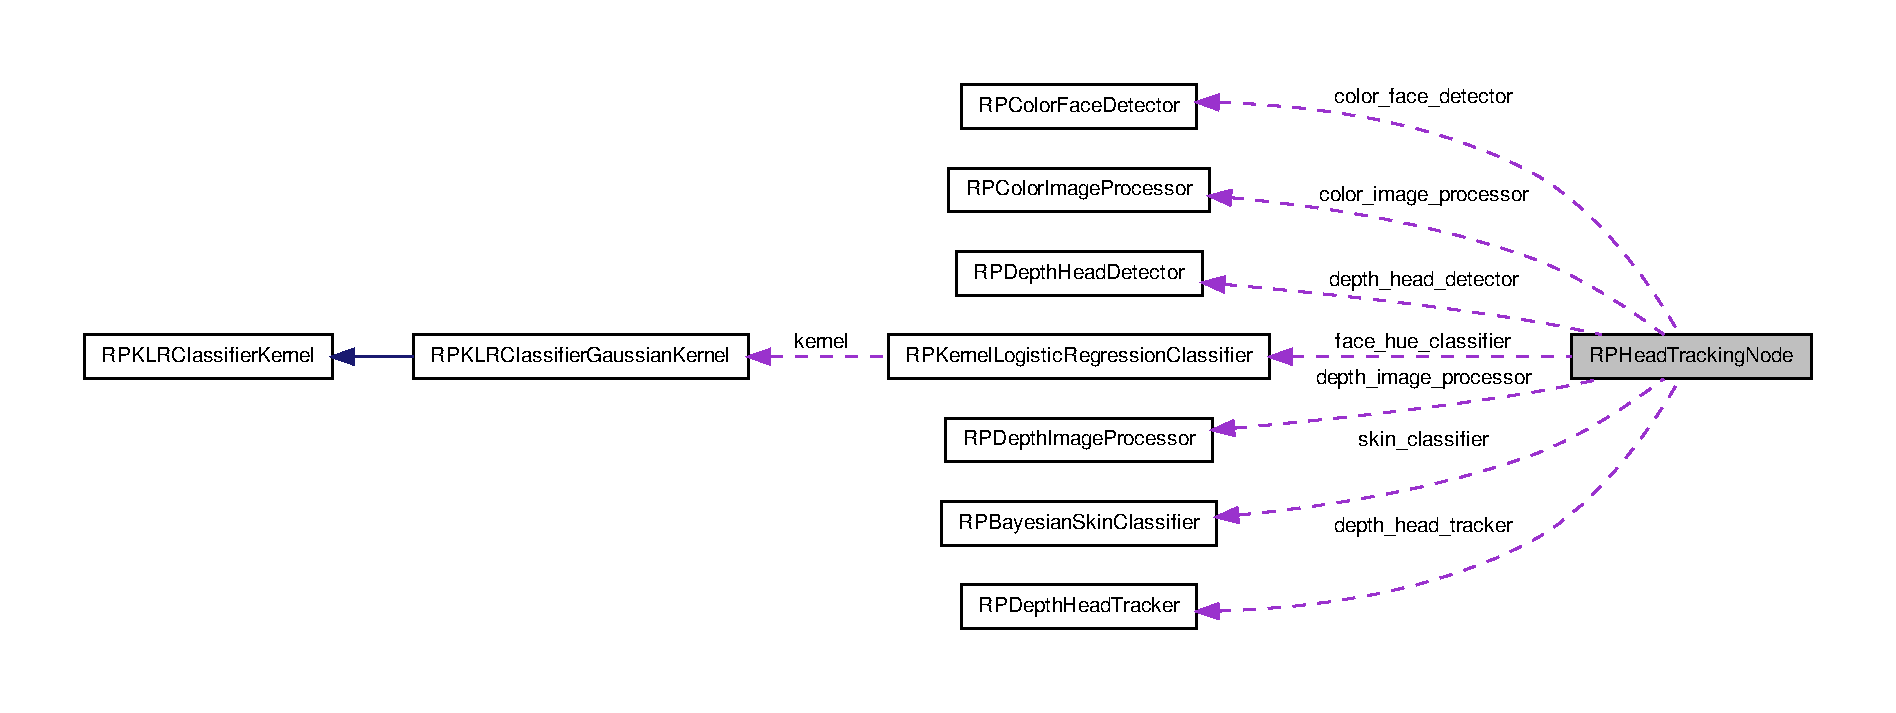
\includegraphics[width=350pt]{class_r_p_head_tracking_node__coll__graph}
\end{center}
\end{figure}
\subsection*{\-Public \-Member \-Functions}
\begin{DoxyCompactItemize}
\item 
\hyperlink{class_r_p_head_tracking_node_a08916811b44ea1c237c5ec607a37cc19}{\-R\-P\-Head\-Tracking\-Node} (ros\-::\-Node\-Handle \&\hyperlink{class_r_p_head_tracking_node_a47a74727765d3593c1d235dbd6cc8e34}{node})
\end{DoxyCompactItemize}
\subsection*{\-Private \-Member \-Functions}
\begin{DoxyCompactItemize}
\item 
void \hyperlink{class_r_p_head_tracking_node_a6c538471c6e3cee05aba40395da2cab1}{sensor\-Input\-Callback} (const sensor\-\_\-msgs\-::\-Image\-::\-Const\-Ptr \&depth\-\_\-input\-\_\-image, const sensor\-\_\-msgs\-::\-Image\-::\-Const\-Ptr \&color\-\_\-input\-\_\-image)
\item 
void \hyperlink{class_r_p_head_tracking_node_ac3df16b7bdb28ca965510d3d11a3296c}{detect\-Heads} (const cv\-\_\-bridge\-::\-Cv\-Image\-::\-Ptr \&depth\-\_\-image, const cv\-\_\-bridge\-::\-Cv\-Image\-::\-Ptr \&color\-\_\-image)
\item 
void \hyperlink{class_r_p_head_tracking_node_a96cb4451897d847dbb65da5d0c7ccac4}{detect\-Faces} (const cv\-\_\-bridge\-::\-Cv\-Image\-::\-Const\-Ptr \&color\-\_\-image)
\item 
void \hyperlink{class_r_p_head_tracking_node_a75bafea5dac2bb6e259e7e5dc4fe0c68}{track\-Heads} (const cv\-\_\-bridge\-::\-Cv\-Image\-::\-Ptr \&depth\-\_\-image)
\item 
void \hyperlink{class_r_p_head_tracking_node_a58746f98c78d01ff274c9bb355d4434a}{publish\-Heads} (const cv\-\_\-bridge\-::\-Cv\-Image\-::\-Const\-Ptr \&depth\-\_\-image)
\item 
void \hyperlink{class_r_p_head_tracking_node_ace266a6c4445813c0f005f3e0162a790}{update\-State} (const \-Head\-Tracking\-State \hyperlink{class_r_p_head_tracking_node_abb89a5e3747c9ce5c046381c2e02b226}{state})
\item 
void \hyperlink{class_r_p_head_tracking_node_a4c52f5c1276087c82d7aad6395b7cf39}{get\-Static\-Parameters} ()
\item 
void \hyperlink{class_r_p_head_tracking_node_ac95a0006516c380ec0a3771aa6fe96f7}{get\-Dynamic\-Head\-Detection\-And\-Tracking\-Parameters} ()
\item 
void \hyperlink{class_r_p_head_tracking_node_a8bf1d1dd8705693c57dc3f814114c4a5}{process\-Output\-Window\-Key\-Press} ()
\end{DoxyCompactItemize}
\subsection*{\-Private \-Attributes}
\begin{DoxyCompactItemize}
\item 
const std\-::string \hyperlink{class_r_p_head_tracking_node_a55c8d0690666fd8ed95b0b8352cca591}{\-W\-I\-N\-D\-O\-W\-\_\-\-N\-A\-M\-E}
\item 
bool \hyperlink{class_r_p_head_tracking_node_ae62a4e592ca4c05f2cd232ca745ad5ba}{\-G\-U\-I\-\_\-\-O\-U\-T\-P\-U\-T\-\_\-\-E\-N\-A\-B\-L\-E\-D}
\item 
int \hyperlink{class_r_p_head_tracking_node_a23eeb6a7ede14f9e47535ef7d6a435b0}{\-N\-U\-M\-B\-E\-R\-\_\-\-O\-F\-\_\-\-F\-R\-A\-M\-E\-S\-\_\-\-U\-N\-T\-I\-L\-\_\-\-D\-E\-T\-E\-C\-T\-O\-R\-\_\-\-R\-E\-I\-N\-I\-T\-I\-A\-L\-I\-Z\-A\-T\-I\-O\-N}
\item 
int \hyperlink{class_r_p_head_tracking_node_ad14b7ec4ecf2cb62091289fb530946be}{\-N\-U\-M\-B\-E\-R\-\_\-\-O\-F\-\_\-\-D\-E\-T\-E\-C\-T\-I\-O\-N\-\_\-\-M\-I\-S\-S\-E\-S\-\_\-\-U\-N\-T\-I\-L\-\_\-\-H\-E\-A\-D\-\_\-\-I\-S\-\_\-\-L\-O\-S\-T}
\item 
bool \hyperlink{class_r_p_head_tracking_node_ad53c9b618a197510b7065d3b9b28dcb1}{\-K\-L\-R\-\_\-\-C\-L\-A\-S\-S\-I\-F\-I\-E\-R\-\_\-\-E\-N\-A\-B\-L\-E\-D}
\item 
double \hyperlink{class_r_p_head_tracking_node_a049bad2b64bbfc0cb43b6a913c5e6617}{\-K\-L\-R\-\_\-\-C\-L\-A\-S\-S\-I\-F\-I\-E\-R\-\_\-\-T\-R\-A\-I\-N\-I\-N\-G\-\_\-\-T\-I\-M\-E\-\_\-\-L\-I\-M\-I\-T}
\item 
int \hyperlink{class_r_p_head_tracking_node_a8834e8b4fe75aa2908fd79e4021b0573}{\-F\-A\-C\-E\-\_\-\-H\-U\-E\-\_\-\-S\-A\-M\-P\-L\-E\-S\-\_\-\-L\-I\-M\-I\-T}
\item 
double \hyperlink{class_r_p_head_tracking_node_a9dda8ff66eca7d0622a438b6c3b77fe9}{\-S\-K\-I\-N\-\_\-\-L\-I\-K\-E\-L\-I\-H\-O\-O\-D\-\_\-\-R\-A\-T\-I\-O\-\_\-\-M\-I\-N\-I\-M\-U\-M}
\item 
bool \hyperlink{class_r_p_head_tracking_node_a164b614083d44aac085c856674170506}{\-S\-K\-I\-N\-\_\-\-H\-E\-U\-R\-I\-S\-T\-I\-C\-\_\-\-E\-N\-A\-B\-L\-E\-D}
\item 
bool \hyperlink{class_r_p_head_tracking_node_a70c083e7ca08af282d686198bd16a884}{\-D\-E\-P\-T\-H\-\_\-\-S\-H\-A\-D\-O\-W\-\_\-\-F\-I\-L\-T\-E\-R\-\_\-\-E\-N\-A\-B\-L\-E\-D}
\item 
bool \hyperlink{class_r_p_head_tracking_node_acd8f3bddcd0db71ecda21f4b5a1858ee}{\-S\-M\-O\-O\-T\-H\-I\-N\-G\-\_\-\-F\-I\-L\-T\-E\-R\-\_\-\-E\-N\-A\-B\-L\-E\-D}
\item 
int \hyperlink{class_r_p_head_tracking_node_a0735dfefd230deabd81cc96d145205ed}{\-S\-M\-O\-O\-T\-H\-I\-N\-G\-\_\-\-R\-A\-D\-I\-U\-S}
\item 
volatile bool \hyperlink{class_r_p_head_tracking_node_a1f2845c7ce72d1a8d117caebd1b1024f}{debug\-\_\-view\-\_\-enabled}
\item 
volatile bool \hyperlink{class_r_p_head_tracking_node_a90f29e5f81692d883b535c8ebcbf9cfc}{color\-\_\-view\-\_\-enabled}
\item 
volatile bool \hyperlink{class_r_p_head_tracking_node_ac8289f71606ec26d687bec74d981ff89}{backprojection\-\_\-view\-\_\-enabled}
\item 
ros\-::\-Node\-Handle \& \hyperlink{class_r_p_head_tracking_node_a47a74727765d3593c1d235dbd6cc8e34}{node}
\item 
\-Head\-Tracking\-State \hyperlink{class_r_p_head_tracking_node_abb89a5e3747c9ce5c046381c2e02b226}{state}
\item 
uint32\-\_\-t \hyperlink{class_r_p_head_tracking_node_aec215913fa33464a7fd8e068b8947d61}{current\-\_\-tracking\-\_\-frame\-\_\-number}
\item 
std\-::string \hyperlink{class_r_p_head_tracking_node_aa31ed34346bf9e26ecd127893d7107af}{frame\-\_\-id}
\item 
std\-::vector$<$ \hyperlink{struct_head}{\-Head} $>$ \hyperlink{class_r_p_head_tracking_node_a8f5e4f1e1a4ba7f043b7f35f21a141d2}{heads}
\item 
cv\-::\-Mat \hyperlink{class_r_p_head_tracking_node_a48e694794e0093a3f096cc66519ab2d9}{render\-\_\-image}
\item 
\hyperlink{class_r_p_depth_head_detector}{\-R\-P\-Depth\-Head\-Detector} \hyperlink{class_r_p_head_tracking_node_af8c98fb4b2589bd038006d9f5d682f58}{depth\-\_\-head\-\_\-detector}
\item 
\hyperlink{class_r_p_depth_head_tracker}{\-R\-P\-Depth\-Head\-Tracker} \hyperlink{class_r_p_head_tracking_node_aeb67f2aec1bc4819304ebea3da893c36}{depth\-\_\-head\-\_\-tracker}
\item 
\hyperlink{class_r_p_depth_image_processor}{\-R\-P\-Depth\-Image\-Processor} \hyperlink{class_r_p_head_tracking_node_adf69f6a784f12825b110d0a852954ef9}{depth\-\_\-image\-\_\-processor}
\item 
\hyperlink{class_r_p_color_image_processor}{\-R\-P\-Color\-Image\-Processor} \hyperlink{class_r_p_head_tracking_node_a74e4f88862813f99d7de88bc8b563efb}{color\-\_\-image\-\_\-processor}
\item 
\hyperlink{class_r_p_color_face_detector}{\-R\-P\-Color\-Face\-Detector} \hyperlink{class_r_p_head_tracking_node_a4e92e10df6588934cbebd6011a68aada}{color\-\_\-face\-\_\-detector}
\item 
\hyperlink{class_r_p_kernel_logistic_regression_classifier}{\-R\-P\-Kernel\-Logistic\-Regression\-Classifier} \hyperlink{class_r_p_head_tracking_node_a9753532076085f324715162e3e1da2a6}{face\-\_\-hue\-\_\-classifier}
\item 
int \hyperlink{class_r_p_head_tracking_node_a57e407d25d6c24ebfaa9a612b63b0a07}{face\-\_\-hue\-\_\-sample\-\_\-count}
\item 
\hyperlink{class_r_p_bayesian_skin_classifier}{\-R\-P\-Bayesian\-Skin\-Classifier} \hyperlink{class_r_p_head_tracking_node_a0e3291a73d232c4725902b829cd40b2b}{skin\-\_\-classifier}
\item 
ros\-::\-Publisher \hyperlink{class_r_p_head_tracking_node_ae463557050c7ea460f519106bbecaec2}{heads\-\_\-publisher}
\item 
ros\-::\-Publisher \hyperlink{class_r_p_head_tracking_node_a2d99f169c031cc19c178c74b462c8c43}{state\-\_\-publisher}
\end{DoxyCompactItemize}


\subsection{\-Detailed \-Description}
\-Robot photographer's head tracking node, which uses the colour and depth inputs from \-Kinect to detect and track humans in \-Luke's vicinity. 

\begin{DoxyCopyright}{\-Copyright}
\-Manfredas \-Zabarauskas, 2013. \-All rights reserved. \-This project is released under \-C\-C \-B\-Y-\/\-N\-C-\/\-S\-A (\-Creative \-Commons \-Attribution-\/\-Non\-Commercial-\/\-Share\-Alike) license. 
\end{DoxyCopyright}


\-Definition at line 51 of file head\-\_\-tracking.\-hpp.



\subsection{\-Constructor \& \-Destructor \-Documentation}
\hypertarget{class_r_p_head_tracking_node_a08916811b44ea1c237c5ec607a37cc19}{\index{\-R\-P\-Head\-Tracking\-Node@{\-R\-P\-Head\-Tracking\-Node}!\-R\-P\-Head\-Tracking\-Node@{\-R\-P\-Head\-Tracking\-Node}}
\index{\-R\-P\-Head\-Tracking\-Node@{\-R\-P\-Head\-Tracking\-Node}!RPHeadTrackingNode@{\-R\-P\-Head\-Tracking\-Node}}
\subsubsection[{\-R\-P\-Head\-Tracking\-Node}]{\setlength{\rightskip}{0pt plus 5cm}{\bf \-R\-P\-Head\-Tracking\-Node\-::\-R\-P\-Head\-Tracking\-Node} (
\begin{DoxyParamCaption}
\item[{ros\-::\-Node\-Handle \&}]{node}
\end{DoxyParamCaption}
)}}\label{class_r_p_head_tracking_node_a08916811b44ea1c237c5ec607a37cc19}
\-Default head detection and tracking node's constructor. 
\begin{DoxyParams}{\-Parameters}
{\em node} & \-Handle to \-R\-O\-S node. \\
\hline
\end{DoxyParams}


\-Definition at line 38 of file head\-\_\-tracking.\-cpp.



\subsection{\-Member \-Function \-Documentation}
\hypertarget{class_r_p_head_tracking_node_a96cb4451897d847dbb65da5d0c7ccac4}{\index{\-R\-P\-Head\-Tracking\-Node@{\-R\-P\-Head\-Tracking\-Node}!detect\-Faces@{detect\-Faces}}
\index{detect\-Faces@{detect\-Faces}!RPHeadTrackingNode@{\-R\-P\-Head\-Tracking\-Node}}
\subsubsection[{detect\-Faces}]{\setlength{\rightskip}{0pt plus 5cm}void {\bf \-R\-P\-Head\-Tracking\-Node\-::detect\-Faces} (
\begin{DoxyParamCaption}
\item[{const cv\-\_\-bridge\-::\-Cv\-Image\-::\-Const\-Ptr \&}]{color\-\_\-image}
\end{DoxyParamCaption}
)\hspace{0.3cm}{\ttfamily  \mbox{[}private\mbox{]}}}}\label{class_r_p_head_tracking_node_a96cb4451897d847dbb65da5d0c7ccac4}
\-Detects faces in a given color image. 
\begin{DoxyParams}{\-Parameters}
{\em color\-\_\-image} & \-Input color image. \\
\hline
\end{DoxyParams}


\-Definition at line 351 of file head\-\_\-tracking.\-cpp.

\hypertarget{class_r_p_head_tracking_node_ac3df16b7bdb28ca965510d3d11a3296c}{\index{\-R\-P\-Head\-Tracking\-Node@{\-R\-P\-Head\-Tracking\-Node}!detect\-Heads@{detect\-Heads}}
\index{detect\-Heads@{detect\-Heads}!RPHeadTrackingNode@{\-R\-P\-Head\-Tracking\-Node}}
\subsubsection[{detect\-Heads}]{\setlength{\rightskip}{0pt plus 5cm}void {\bf \-R\-P\-Head\-Tracking\-Node\-::detect\-Heads} (
\begin{DoxyParamCaption}
\item[{const cv\-\_\-bridge\-::\-Cv\-Image\-::\-Ptr \&}]{depth\-\_\-image, }
\item[{const cv\-\_\-bridge\-::\-Cv\-Image\-::\-Ptr \&}]{color\-\_\-image}
\end{DoxyParamCaption}
)\hspace{0.3cm}{\ttfamily  \mbox{[}private\mbox{]}}}}\label{class_r_p_head_tracking_node_ac3df16b7bdb28ca965510d3d11a3296c}
\-Detects heads in a given depth image (potentially using color cues for detected head verification). 
\begin{DoxyParams}{\-Parameters}
{\em depth\-\_\-image} & \-Input depth image. \\
\hline
{\em color\-\_\-image} & \-Input color image. \\
\hline
\end{DoxyParams}


\-Definition at line 246 of file head\-\_\-tracking.\-cpp.

\hypertarget{class_r_p_head_tracking_node_ac95a0006516c380ec0a3771aa6fe96f7}{\index{\-R\-P\-Head\-Tracking\-Node@{\-R\-P\-Head\-Tracking\-Node}!get\-Dynamic\-Head\-Detection\-And\-Tracking\-Parameters@{get\-Dynamic\-Head\-Detection\-And\-Tracking\-Parameters}}
\index{get\-Dynamic\-Head\-Detection\-And\-Tracking\-Parameters@{get\-Dynamic\-Head\-Detection\-And\-Tracking\-Parameters}!RPHeadTrackingNode@{\-R\-P\-Head\-Tracking\-Node}}
\subsubsection[{get\-Dynamic\-Head\-Detection\-And\-Tracking\-Parameters}]{\setlength{\rightskip}{0pt plus 5cm}void {\bf \-R\-P\-Head\-Tracking\-Node\-::get\-Dynamic\-Head\-Detection\-And\-Tracking\-Parameters} (
\begin{DoxyParamCaption}
{}
\end{DoxyParamCaption}
)\hspace{0.3cm}{\ttfamily  \mbox{[}private\mbox{]}}}}\label{class_r_p_head_tracking_node_ac95a0006516c380ec0a3771aa6fe96f7}
\-Gets dynamic head detection and tracking overridable parameters from the parameter server. 

\-Definition at line 115 of file head\-\_\-tracking.\-cpp.

\hypertarget{class_r_p_head_tracking_node_a4c52f5c1276087c82d7aad6395b7cf39}{\index{\-R\-P\-Head\-Tracking\-Node@{\-R\-P\-Head\-Tracking\-Node}!get\-Static\-Parameters@{get\-Static\-Parameters}}
\index{get\-Static\-Parameters@{get\-Static\-Parameters}!RPHeadTrackingNode@{\-R\-P\-Head\-Tracking\-Node}}
\subsubsection[{get\-Static\-Parameters}]{\setlength{\rightskip}{0pt plus 5cm}void {\bf \-R\-P\-Head\-Tracking\-Node\-::get\-Static\-Parameters} (
\begin{DoxyParamCaption}
{}
\end{DoxyParamCaption}
)\hspace{0.3cm}{\ttfamily  \mbox{[}private\mbox{]}}}}\label{class_r_p_head_tracking_node_a4c52f5c1276087c82d7aad6395b7cf39}
\-Gets static overridable parameters from the parameter server. 

\-Definition at line 104 of file head\-\_\-tracking.\-cpp.

\hypertarget{class_r_p_head_tracking_node_a8bf1d1dd8705693c57dc3f814114c4a5}{\index{\-R\-P\-Head\-Tracking\-Node@{\-R\-P\-Head\-Tracking\-Node}!process\-Output\-Window\-Key\-Press@{process\-Output\-Window\-Key\-Press}}
\index{process\-Output\-Window\-Key\-Press@{process\-Output\-Window\-Key\-Press}!RPHeadTrackingNode@{\-R\-P\-Head\-Tracking\-Node}}
\subsubsection[{process\-Output\-Window\-Key\-Press}]{\setlength{\rightskip}{0pt plus 5cm}void {\bf \-R\-P\-Head\-Tracking\-Node\-::process\-Output\-Window\-Key\-Press} (
\begin{DoxyParamCaption}
{}
\end{DoxyParamCaption}
)\hspace{0.3cm}{\ttfamily  \mbox{[}private\mbox{]}}}}\label{class_r_p_head_tracking_node_a8bf1d1dd8705693c57dc3f814114c4a5}
\-Processes key presses for the \-G\-U\-I output window. 

\-Definition at line 420 of file head\-\_\-tracking.\-cpp.

\hypertarget{class_r_p_head_tracking_node_a58746f98c78d01ff274c9bb355d4434a}{\index{\-R\-P\-Head\-Tracking\-Node@{\-R\-P\-Head\-Tracking\-Node}!publish\-Heads@{publish\-Heads}}
\index{publish\-Heads@{publish\-Heads}!RPHeadTrackingNode@{\-R\-P\-Head\-Tracking\-Node}}
\subsubsection[{publish\-Heads}]{\setlength{\rightskip}{0pt plus 5cm}void {\bf \-R\-P\-Head\-Tracking\-Node\-::publish\-Heads} (
\begin{DoxyParamCaption}
\item[{const cv\-\_\-bridge\-::\-Cv\-Image\-::\-Const\-Ptr \&}]{depth\-\_\-image}
\end{DoxyParamCaption}
)\hspace{0.3cm}{\ttfamily  \mbox{[}private\mbox{]}}}}\label{class_r_p_head_tracking_node_a58746f98c78d01ff274c9bb355d4434a}
\-Publishes detected/tracked heads in a current depth image. 
\begin{DoxyParams}{\-Parameters}
{\em depth\-\_\-image} & \-Current depth image. \\
\hline
\end{DoxyParams}


\-Definition at line 231 of file head\-\_\-tracking.\-cpp.

\hypertarget{class_r_p_head_tracking_node_a6c538471c6e3cee05aba40395da2cab1}{\index{\-R\-P\-Head\-Tracking\-Node@{\-R\-P\-Head\-Tracking\-Node}!sensor\-Input\-Callback@{sensor\-Input\-Callback}}
\index{sensor\-Input\-Callback@{sensor\-Input\-Callback}!RPHeadTrackingNode@{\-R\-P\-Head\-Tracking\-Node}}
\subsubsection[{sensor\-Input\-Callback}]{\setlength{\rightskip}{0pt plus 5cm}void {\bf \-R\-P\-Head\-Tracking\-Node\-::sensor\-Input\-Callback} (
\begin{DoxyParamCaption}
\item[{const sensor\-\_\-msgs\-::\-Image\-::\-Const\-Ptr \&}]{depth\-\_\-input\-\_\-image, }
\item[{const sensor\-\_\-msgs\-::\-Image\-::\-Const\-Ptr \&}]{color\-\_\-input\-\_\-image}
\end{DoxyParamCaption}
)\hspace{0.3cm}{\ttfamily  \mbox{[}private\mbox{]}}}}\label{class_r_p_head_tracking_node_a6c538471c6e3cee05aba40395da2cab1}
\-Callback for the depth and color inputs from \-R\-G\-B-\/\-D sensor. 
\begin{DoxyParams}{\-Parameters}
{\em depth\-\_\-input\-\_\-image} & \-Input depth image. \\
\hline
{\em color\-\_\-input\-\_\-image} & \-Input color image. \\
\hline
\end{DoxyParams}


\-Definition at line 125 of file head\-\_\-tracking.\-cpp.

\hypertarget{class_r_p_head_tracking_node_a75bafea5dac2bb6e259e7e5dc4fe0c68}{\index{\-R\-P\-Head\-Tracking\-Node@{\-R\-P\-Head\-Tracking\-Node}!track\-Heads@{track\-Heads}}
\index{track\-Heads@{track\-Heads}!RPHeadTrackingNode@{\-R\-P\-Head\-Tracking\-Node}}
\subsubsection[{track\-Heads}]{\setlength{\rightskip}{0pt plus 5cm}void {\bf \-R\-P\-Head\-Tracking\-Node\-::track\-Heads} (
\begin{DoxyParamCaption}
\item[{const cv\-\_\-bridge\-::\-Cv\-Image\-::\-Ptr \&}]{depth\-\_\-image}
\end{DoxyParamCaption}
)\hspace{0.3cm}{\ttfamily  \mbox{[}private\mbox{]}}}}\label{class_r_p_head_tracking_node_a75bafea5dac2bb6e259e7e5dc4fe0c68}
\-Tracks detected heads in a given depth image. 
\begin{DoxyParams}{\-Parameters}
{\em depth\-\_\-image} & \-Input depth image. \\
\hline
\end{DoxyParams}


\-Definition at line 388 of file head\-\_\-tracking.\-cpp.

\hypertarget{class_r_p_head_tracking_node_ace266a6c4445813c0f005f3e0162a790}{\index{\-R\-P\-Head\-Tracking\-Node@{\-R\-P\-Head\-Tracking\-Node}!update\-State@{update\-State}}
\index{update\-State@{update\-State}!RPHeadTrackingNode@{\-R\-P\-Head\-Tracking\-Node}}
\subsubsection[{update\-State}]{\setlength{\rightskip}{0pt plus 5cm}void {\bf \-R\-P\-Head\-Tracking\-Node\-::update\-State} (
\begin{DoxyParamCaption}
\item[{const \-Head\-Tracking\-State}]{state}
\end{DoxyParamCaption}
)\hspace{0.3cm}{\ttfamily  \mbox{[}private\mbox{]}}}}\label{class_r_p_head_tracking_node_ace266a6c4445813c0f005f3e0162a790}
\-Updates the node's state. 
\begin{DoxyParams}{\-Parameters}
{\em state} & \-Desired new state. \\
\hline
\end{DoxyParams}


\-Definition at line 220 of file head\-\_\-tracking.\-cpp.



\subsection{\-Member \-Data \-Documentation}
\hypertarget{class_r_p_head_tracking_node_ac8289f71606ec26d687bec74d981ff89}{\index{\-R\-P\-Head\-Tracking\-Node@{\-R\-P\-Head\-Tracking\-Node}!backprojection\-\_\-view\-\_\-enabled@{backprojection\-\_\-view\-\_\-enabled}}
\index{backprojection\-\_\-view\-\_\-enabled@{backprojection\-\_\-view\-\_\-enabled}!RPHeadTrackingNode@{\-R\-P\-Head\-Tracking\-Node}}
\subsubsection[{backprojection\-\_\-view\-\_\-enabled}]{\setlength{\rightskip}{0pt plus 5cm}volatile bool {\bf \-R\-P\-Head\-Tracking\-Node\-::backprojection\-\_\-view\-\_\-enabled}\hspace{0.3cm}{\ttfamily  \mbox{[}private\mbox{]}}}}\label{class_r_p_head_tracking_node_ac8289f71606ec26d687bec74d981ff89}
\-Skin probability backprojection view enabled flag. 

\-Definition at line 84 of file head\-\_\-tracking.\-hpp.

\hypertarget{class_r_p_head_tracking_node_a4e92e10df6588934cbebd6011a68aada}{\index{\-R\-P\-Head\-Tracking\-Node@{\-R\-P\-Head\-Tracking\-Node}!color\-\_\-face\-\_\-detector@{color\-\_\-face\-\_\-detector}}
\index{color\-\_\-face\-\_\-detector@{color\-\_\-face\-\_\-detector}!RPHeadTrackingNode@{\-R\-P\-Head\-Tracking\-Node}}
\subsubsection[{color\-\_\-face\-\_\-detector}]{\setlength{\rightskip}{0pt plus 5cm}{\bf \-R\-P\-Color\-Face\-Detector} {\bf \-R\-P\-Head\-Tracking\-Node\-::color\-\_\-face\-\_\-detector}\hspace{0.3cm}{\ttfamily  \mbox{[}private\mbox{]}}}}\label{class_r_p_head_tracking_node_a4e92e10df6588934cbebd6011a68aada}
\-Face detector from color data. 

\-Definition at line 100 of file head\-\_\-tracking.\-hpp.

\hypertarget{class_r_p_head_tracking_node_a74e4f88862813f99d7de88bc8b563efb}{\index{\-R\-P\-Head\-Tracking\-Node@{\-R\-P\-Head\-Tracking\-Node}!color\-\_\-image\-\_\-processor@{color\-\_\-image\-\_\-processor}}
\index{color\-\_\-image\-\_\-processor@{color\-\_\-image\-\_\-processor}!RPHeadTrackingNode@{\-R\-P\-Head\-Tracking\-Node}}
\subsubsection[{color\-\_\-image\-\_\-processor}]{\setlength{\rightskip}{0pt plus 5cm}{\bf \-R\-P\-Color\-Image\-Processor} {\bf \-R\-P\-Head\-Tracking\-Node\-::color\-\_\-image\-\_\-processor}\hspace{0.3cm}{\ttfamily  \mbox{[}private\mbox{]}}}}\label{class_r_p_head_tracking_node_a74e4f88862813f99d7de88bc8b563efb}
\-Color image processor. 

\-Definition at line 99 of file head\-\_\-tracking.\-hpp.

\hypertarget{class_r_p_head_tracking_node_a90f29e5f81692d883b535c8ebcbf9cfc}{\index{\-R\-P\-Head\-Tracking\-Node@{\-R\-P\-Head\-Tracking\-Node}!color\-\_\-view\-\_\-enabled@{color\-\_\-view\-\_\-enabled}}
\index{color\-\_\-view\-\_\-enabled@{color\-\_\-view\-\_\-enabled}!RPHeadTrackingNode@{\-R\-P\-Head\-Tracking\-Node}}
\subsubsection[{color\-\_\-view\-\_\-enabled}]{\setlength{\rightskip}{0pt plus 5cm}volatile bool {\bf \-R\-P\-Head\-Tracking\-Node\-::color\-\_\-view\-\_\-enabled}\hspace{0.3cm}{\ttfamily  \mbox{[}private\mbox{]}}}}\label{class_r_p_head_tracking_node_a90f29e5f81692d883b535c8ebcbf9cfc}
\-Color view enabled flag. 

\-Definition at line 83 of file head\-\_\-tracking.\-hpp.

\hypertarget{class_r_p_head_tracking_node_aec215913fa33464a7fd8e068b8947d61}{\index{\-R\-P\-Head\-Tracking\-Node@{\-R\-P\-Head\-Tracking\-Node}!current\-\_\-tracking\-\_\-frame\-\_\-number@{current\-\_\-tracking\-\_\-frame\-\_\-number}}
\index{current\-\_\-tracking\-\_\-frame\-\_\-number@{current\-\_\-tracking\-\_\-frame\-\_\-number}!RPHeadTrackingNode@{\-R\-P\-Head\-Tracking\-Node}}
\subsubsection[{current\-\_\-tracking\-\_\-frame\-\_\-number}]{\setlength{\rightskip}{0pt plus 5cm}uint32\-\_\-t {\bf \-R\-P\-Head\-Tracking\-Node\-::current\-\_\-tracking\-\_\-frame\-\_\-number}\hspace{0.3cm}{\ttfamily  \mbox{[}private\mbox{]}}}}\label{class_r_p_head_tracking_node_aec215913fa33464a7fd8e068b8947d61}
\-Current frame number. 

\-Definition at line 89 of file head\-\_\-tracking.\-hpp.

\hypertarget{class_r_p_head_tracking_node_a1f2845c7ce72d1a8d117caebd1b1024f}{\index{\-R\-P\-Head\-Tracking\-Node@{\-R\-P\-Head\-Tracking\-Node}!debug\-\_\-view\-\_\-enabled@{debug\-\_\-view\-\_\-enabled}}
\index{debug\-\_\-view\-\_\-enabled@{debug\-\_\-view\-\_\-enabled}!RPHeadTrackingNode@{\-R\-P\-Head\-Tracking\-Node}}
\subsubsection[{debug\-\_\-view\-\_\-enabled}]{\setlength{\rightskip}{0pt plus 5cm}volatile bool {\bf \-R\-P\-Head\-Tracking\-Node\-::debug\-\_\-view\-\_\-enabled}\hspace{0.3cm}{\ttfamily  \mbox{[}private\mbox{]}}}}\label{class_r_p_head_tracking_node_a1f2845c7ce72d1a8d117caebd1b1024f}
\-Debug view enabled flag. 

\-Definition at line 82 of file head\-\_\-tracking.\-hpp.

\hypertarget{class_r_p_head_tracking_node_af8c98fb4b2589bd038006d9f5d682f58}{\index{\-R\-P\-Head\-Tracking\-Node@{\-R\-P\-Head\-Tracking\-Node}!depth\-\_\-head\-\_\-detector@{depth\-\_\-head\-\_\-detector}}
\index{depth\-\_\-head\-\_\-detector@{depth\-\_\-head\-\_\-detector}!RPHeadTrackingNode@{\-R\-P\-Head\-Tracking\-Node}}
\subsubsection[{depth\-\_\-head\-\_\-detector}]{\setlength{\rightskip}{0pt plus 5cm}{\bf \-R\-P\-Depth\-Head\-Detector} {\bf \-R\-P\-Head\-Tracking\-Node\-::depth\-\_\-head\-\_\-detector}\hspace{0.3cm}{\ttfamily  \mbox{[}private\mbox{]}}}}\label{class_r_p_head_tracking_node_af8c98fb4b2589bd038006d9f5d682f58}
\hyperlink{struct_head}{\-Head} detector from depth data. 

\-Definition at line 96 of file head\-\_\-tracking.\-hpp.

\hypertarget{class_r_p_head_tracking_node_aeb67f2aec1bc4819304ebea3da893c36}{\index{\-R\-P\-Head\-Tracking\-Node@{\-R\-P\-Head\-Tracking\-Node}!depth\-\_\-head\-\_\-tracker@{depth\-\_\-head\-\_\-tracker}}
\index{depth\-\_\-head\-\_\-tracker@{depth\-\_\-head\-\_\-tracker}!RPHeadTrackingNode@{\-R\-P\-Head\-Tracking\-Node}}
\subsubsection[{depth\-\_\-head\-\_\-tracker}]{\setlength{\rightskip}{0pt plus 5cm}{\bf \-R\-P\-Depth\-Head\-Tracker} {\bf \-R\-P\-Head\-Tracking\-Node\-::depth\-\_\-head\-\_\-tracker}\hspace{0.3cm}{\ttfamily  \mbox{[}private\mbox{]}}}}\label{class_r_p_head_tracking_node_aeb67f2aec1bc4819304ebea3da893c36}
\hyperlink{struct_head}{\-Head} tracker using depth data. 

\-Definition at line 97 of file head\-\_\-tracking.\-hpp.

\hypertarget{class_r_p_head_tracking_node_adf69f6a784f12825b110d0a852954ef9}{\index{\-R\-P\-Head\-Tracking\-Node@{\-R\-P\-Head\-Tracking\-Node}!depth\-\_\-image\-\_\-processor@{depth\-\_\-image\-\_\-processor}}
\index{depth\-\_\-image\-\_\-processor@{depth\-\_\-image\-\_\-processor}!RPHeadTrackingNode@{\-R\-P\-Head\-Tracking\-Node}}
\subsubsection[{depth\-\_\-image\-\_\-processor}]{\setlength{\rightskip}{0pt plus 5cm}{\bf \-R\-P\-Depth\-Image\-Processor} {\bf \-R\-P\-Head\-Tracking\-Node\-::depth\-\_\-image\-\_\-processor}\hspace{0.3cm}{\ttfamily  \mbox{[}private\mbox{]}}}}\label{class_r_p_head_tracking_node_adf69f6a784f12825b110d0a852954ef9}
\-Depth image processor. 

\-Definition at line 98 of file head\-\_\-tracking.\-hpp.

\hypertarget{class_r_p_head_tracking_node_a70c083e7ca08af282d686198bd16a884}{\index{\-R\-P\-Head\-Tracking\-Node@{\-R\-P\-Head\-Tracking\-Node}!\-D\-E\-P\-T\-H\-\_\-\-S\-H\-A\-D\-O\-W\-\_\-\-F\-I\-L\-T\-E\-R\-\_\-\-E\-N\-A\-B\-L\-E\-D@{\-D\-E\-P\-T\-H\-\_\-\-S\-H\-A\-D\-O\-W\-\_\-\-F\-I\-L\-T\-E\-R\-\_\-\-E\-N\-A\-B\-L\-E\-D}}
\index{\-D\-E\-P\-T\-H\-\_\-\-S\-H\-A\-D\-O\-W\-\_\-\-F\-I\-L\-T\-E\-R\-\_\-\-E\-N\-A\-B\-L\-E\-D@{\-D\-E\-P\-T\-H\-\_\-\-S\-H\-A\-D\-O\-W\-\_\-\-F\-I\-L\-T\-E\-R\-\_\-\-E\-N\-A\-B\-L\-E\-D}!RPHeadTrackingNode@{\-R\-P\-Head\-Tracking\-Node}}
\subsubsection[{\-D\-E\-P\-T\-H\-\_\-\-S\-H\-A\-D\-O\-W\-\_\-\-F\-I\-L\-T\-E\-R\-\_\-\-E\-N\-A\-B\-L\-E\-D}]{\setlength{\rightskip}{0pt plus 5cm}bool {\bf \-R\-P\-Head\-Tracking\-Node\-::\-D\-E\-P\-T\-H\-\_\-\-S\-H\-A\-D\-O\-W\-\_\-\-F\-I\-L\-T\-E\-R\-\_\-\-E\-N\-A\-B\-L\-E\-D}\hspace{0.3cm}{\ttfamily  \mbox{[}private\mbox{]}}}}\label{class_r_p_head_tracking_node_a70c083e7ca08af282d686198bd16a884}
\-Depth shadow filter enabled flag \-O\-P. 

\-Definition at line 75 of file head\-\_\-tracking.\-hpp.

\hypertarget{class_r_p_head_tracking_node_a9753532076085f324715162e3e1da2a6}{\index{\-R\-P\-Head\-Tracking\-Node@{\-R\-P\-Head\-Tracking\-Node}!face\-\_\-hue\-\_\-classifier@{face\-\_\-hue\-\_\-classifier}}
\index{face\-\_\-hue\-\_\-classifier@{face\-\_\-hue\-\_\-classifier}!RPHeadTrackingNode@{\-R\-P\-Head\-Tracking\-Node}}
\subsubsection[{face\-\_\-hue\-\_\-classifier}]{\setlength{\rightskip}{0pt plus 5cm}{\bf \-R\-P\-Kernel\-Logistic\-Regression\-Classifier} {\bf \-R\-P\-Head\-Tracking\-Node\-::face\-\_\-hue\-\_\-classifier}\hspace{0.3cm}{\ttfamily  \mbox{[}private\mbox{]}}}}\label{class_r_p_head_tracking_node_a9753532076085f324715162e3e1da2a6}
\-Kernel logistic regression classifier for face/non-\/face hue classification. 

\-Definition at line 101 of file head\-\_\-tracking.\-hpp.

\hypertarget{class_r_p_head_tracking_node_a57e407d25d6c24ebfaa9a612b63b0a07}{\index{\-R\-P\-Head\-Tracking\-Node@{\-R\-P\-Head\-Tracking\-Node}!face\-\_\-hue\-\_\-sample\-\_\-count@{face\-\_\-hue\-\_\-sample\-\_\-count}}
\index{face\-\_\-hue\-\_\-sample\-\_\-count@{face\-\_\-hue\-\_\-sample\-\_\-count}!RPHeadTrackingNode@{\-R\-P\-Head\-Tracking\-Node}}
\subsubsection[{face\-\_\-hue\-\_\-sample\-\_\-count}]{\setlength{\rightskip}{0pt plus 5cm}int {\bf \-R\-P\-Head\-Tracking\-Node\-::face\-\_\-hue\-\_\-sample\-\_\-count}\hspace{0.3cm}{\ttfamily  \mbox{[}private\mbox{]}}}}\label{class_r_p_head_tracking_node_a57e407d25d6c24ebfaa9a612b63b0a07}
\-Gathered face hue sample count. 

\-Definition at line 104 of file head\-\_\-tracking.\-hpp.

\hypertarget{class_r_p_head_tracking_node_a8834e8b4fe75aa2908fd79e4021b0573}{\index{\-R\-P\-Head\-Tracking\-Node@{\-R\-P\-Head\-Tracking\-Node}!\-F\-A\-C\-E\-\_\-\-H\-U\-E\-\_\-\-S\-A\-M\-P\-L\-E\-S\-\_\-\-L\-I\-M\-I\-T@{\-F\-A\-C\-E\-\_\-\-H\-U\-E\-\_\-\-S\-A\-M\-P\-L\-E\-S\-\_\-\-L\-I\-M\-I\-T}}
\index{\-F\-A\-C\-E\-\_\-\-H\-U\-E\-\_\-\-S\-A\-M\-P\-L\-E\-S\-\_\-\-L\-I\-M\-I\-T@{\-F\-A\-C\-E\-\_\-\-H\-U\-E\-\_\-\-S\-A\-M\-P\-L\-E\-S\-\_\-\-L\-I\-M\-I\-T}!RPHeadTrackingNode@{\-R\-P\-Head\-Tracking\-Node}}
\subsubsection[{\-F\-A\-C\-E\-\_\-\-H\-U\-E\-\_\-\-S\-A\-M\-P\-L\-E\-S\-\_\-\-L\-I\-M\-I\-T}]{\setlength{\rightskip}{0pt plus 5cm}int {\bf \-R\-P\-Head\-Tracking\-Node\-::\-F\-A\-C\-E\-\_\-\-H\-U\-E\-\_\-\-S\-A\-M\-P\-L\-E\-S\-\_\-\-L\-I\-M\-I\-T}\hspace{0.3cm}{\ttfamily  \mbox{[}private\mbox{]}}}}\label{class_r_p_head_tracking_node_a8834e8b4fe75aa2908fd79e4021b0573}
\-Face hue sample limit \-O\-P for \-K\-L\-R classifier training. 

\-Definition at line 67 of file head\-\_\-tracking.\-hpp.

\hypertarget{class_r_p_head_tracking_node_aa31ed34346bf9e26ecd127893d7107af}{\index{\-R\-P\-Head\-Tracking\-Node@{\-R\-P\-Head\-Tracking\-Node}!frame\-\_\-id@{frame\-\_\-id}}
\index{frame\-\_\-id@{frame\-\_\-id}!RPHeadTrackingNode@{\-R\-P\-Head\-Tracking\-Node}}
\subsubsection[{frame\-\_\-id}]{\setlength{\rightskip}{0pt plus 5cm}std\-::string {\bf \-R\-P\-Head\-Tracking\-Node\-::frame\-\_\-id}\hspace{0.3cm}{\ttfamily  \mbox{[}private\mbox{]}}}}\label{class_r_p_head_tracking_node_aa31ed34346bf9e26ecd127893d7107af}
\-Frame \-I\-D (same as \-Kinect's \-R\-G\-B camera \-I\-D). 

\-Definition at line 90 of file head\-\_\-tracking.\-hpp.

\hypertarget{class_r_p_head_tracking_node_ae62a4e592ca4c05f2cd232ca745ad5ba}{\index{\-R\-P\-Head\-Tracking\-Node@{\-R\-P\-Head\-Tracking\-Node}!\-G\-U\-I\-\_\-\-O\-U\-T\-P\-U\-T\-\_\-\-E\-N\-A\-B\-L\-E\-D@{\-G\-U\-I\-\_\-\-O\-U\-T\-P\-U\-T\-\_\-\-E\-N\-A\-B\-L\-E\-D}}
\index{\-G\-U\-I\-\_\-\-O\-U\-T\-P\-U\-T\-\_\-\-E\-N\-A\-B\-L\-E\-D@{\-G\-U\-I\-\_\-\-O\-U\-T\-P\-U\-T\-\_\-\-E\-N\-A\-B\-L\-E\-D}!RPHeadTrackingNode@{\-R\-P\-Head\-Tracking\-Node}}
\subsubsection[{\-G\-U\-I\-\_\-\-O\-U\-T\-P\-U\-T\-\_\-\-E\-N\-A\-B\-L\-E\-D}]{\setlength{\rightskip}{0pt plus 5cm}bool {\bf \-R\-P\-Head\-Tracking\-Node\-::\-G\-U\-I\-\_\-\-O\-U\-T\-P\-U\-T\-\_\-\-E\-N\-A\-B\-L\-E\-D}\hspace{0.3cm}{\ttfamily  \mbox{[}private\mbox{]}}}}\label{class_r_p_head_tracking_node_ae62a4e592ca4c05f2cd232ca745ad5ba}
\-G\-U\-I output enabled flag \-O\-P. 

\-Definition at line 56 of file head\-\_\-tracking.\-hpp.

\hypertarget{class_r_p_head_tracking_node_a8f5e4f1e1a4ba7f043b7f35f21a141d2}{\index{\-R\-P\-Head\-Tracking\-Node@{\-R\-P\-Head\-Tracking\-Node}!heads@{heads}}
\index{heads@{heads}!RPHeadTrackingNode@{\-R\-P\-Head\-Tracking\-Node}}
\subsubsection[{heads}]{\setlength{\rightskip}{0pt plus 5cm}std\-::vector$<${\bf \-Head}$>$ {\bf \-R\-P\-Head\-Tracking\-Node\-::heads}\hspace{0.3cm}{\ttfamily  \mbox{[}private\mbox{]}}}}\label{class_r_p_head_tracking_node_a8f5e4f1e1a4ba7f043b7f35f21a141d2}
\-Detected/tracked head rectangles. 

\-Definition at line 92 of file head\-\_\-tracking.\-hpp.

\hypertarget{class_r_p_head_tracking_node_ae463557050c7ea460f519106bbecaec2}{\index{\-R\-P\-Head\-Tracking\-Node@{\-R\-P\-Head\-Tracking\-Node}!heads\-\_\-publisher@{heads\-\_\-publisher}}
\index{heads\-\_\-publisher@{heads\-\_\-publisher}!RPHeadTrackingNode@{\-R\-P\-Head\-Tracking\-Node}}
\subsubsection[{heads\-\_\-publisher}]{\setlength{\rightskip}{0pt plus 5cm}ros\-::\-Publisher {\bf \-R\-P\-Head\-Tracking\-Node\-::heads\-\_\-publisher}\hspace{0.3cm}{\ttfamily  \mbox{[}private\mbox{]}}}}\label{class_r_p_head_tracking_node_ae463557050c7ea460f519106bbecaec2}
\-Detected heads publisher. 

\-Definition at line 107 of file head\-\_\-tracking.\-hpp.

\hypertarget{class_r_p_head_tracking_node_ad53c9b618a197510b7065d3b9b28dcb1}{\index{\-R\-P\-Head\-Tracking\-Node@{\-R\-P\-Head\-Tracking\-Node}!\-K\-L\-R\-\_\-\-C\-L\-A\-S\-S\-I\-F\-I\-E\-R\-\_\-\-E\-N\-A\-B\-L\-E\-D@{\-K\-L\-R\-\_\-\-C\-L\-A\-S\-S\-I\-F\-I\-E\-R\-\_\-\-E\-N\-A\-B\-L\-E\-D}}
\index{\-K\-L\-R\-\_\-\-C\-L\-A\-S\-S\-I\-F\-I\-E\-R\-\_\-\-E\-N\-A\-B\-L\-E\-D@{\-K\-L\-R\-\_\-\-C\-L\-A\-S\-S\-I\-F\-I\-E\-R\-\_\-\-E\-N\-A\-B\-L\-E\-D}!RPHeadTrackingNode@{\-R\-P\-Head\-Tracking\-Node}}
\subsubsection[{\-K\-L\-R\-\_\-\-C\-L\-A\-S\-S\-I\-F\-I\-E\-R\-\_\-\-E\-N\-A\-B\-L\-E\-D}]{\setlength{\rightskip}{0pt plus 5cm}bool {\bf \-R\-P\-Head\-Tracking\-Node\-::\-K\-L\-R\-\_\-\-C\-L\-A\-S\-S\-I\-F\-I\-E\-R\-\_\-\-E\-N\-A\-B\-L\-E\-D}\hspace{0.3cm}{\ttfamily  \mbox{[}private\mbox{]}}}}\label{class_r_p_head_tracking_node_ad53c9b618a197510b7065d3b9b28dcb1}
\-K\-L\-R classifier enabled \-O\-P. 

\-Definition at line 64 of file head\-\_\-tracking.\-hpp.

\hypertarget{class_r_p_head_tracking_node_a049bad2b64bbfc0cb43b6a913c5e6617}{\index{\-R\-P\-Head\-Tracking\-Node@{\-R\-P\-Head\-Tracking\-Node}!\-K\-L\-R\-\_\-\-C\-L\-A\-S\-S\-I\-F\-I\-E\-R\-\_\-\-T\-R\-A\-I\-N\-I\-N\-G\-\_\-\-T\-I\-M\-E\-\_\-\-L\-I\-M\-I\-T@{\-K\-L\-R\-\_\-\-C\-L\-A\-S\-S\-I\-F\-I\-E\-R\-\_\-\-T\-R\-A\-I\-N\-I\-N\-G\-\_\-\-T\-I\-M\-E\-\_\-\-L\-I\-M\-I\-T}}
\index{\-K\-L\-R\-\_\-\-C\-L\-A\-S\-S\-I\-F\-I\-E\-R\-\_\-\-T\-R\-A\-I\-N\-I\-N\-G\-\_\-\-T\-I\-M\-E\-\_\-\-L\-I\-M\-I\-T@{\-K\-L\-R\-\_\-\-C\-L\-A\-S\-S\-I\-F\-I\-E\-R\-\_\-\-T\-R\-A\-I\-N\-I\-N\-G\-\_\-\-T\-I\-M\-E\-\_\-\-L\-I\-M\-I\-T}!RPHeadTrackingNode@{\-R\-P\-Head\-Tracking\-Node}}
\subsubsection[{\-K\-L\-R\-\_\-\-C\-L\-A\-S\-S\-I\-F\-I\-E\-R\-\_\-\-T\-R\-A\-I\-N\-I\-N\-G\-\_\-\-T\-I\-M\-E\-\_\-\-L\-I\-M\-I\-T}]{\setlength{\rightskip}{0pt plus 5cm}double {\bf \-R\-P\-Head\-Tracking\-Node\-::\-K\-L\-R\-\_\-\-C\-L\-A\-S\-S\-I\-F\-I\-E\-R\-\_\-\-T\-R\-A\-I\-N\-I\-N\-G\-\_\-\-T\-I\-M\-E\-\_\-\-L\-I\-M\-I\-T}\hspace{0.3cm}{\ttfamily  \mbox{[}private\mbox{]}}}}\label{class_r_p_head_tracking_node_a049bad2b64bbfc0cb43b6a913c5e6617}
\-K\-L\-R classifier training time limit \-O\-P. 

\-Definition at line 65 of file head\-\_\-tracking.\-hpp.

\hypertarget{class_r_p_head_tracking_node_a47a74727765d3593c1d235dbd6cc8e34}{\index{\-R\-P\-Head\-Tracking\-Node@{\-R\-P\-Head\-Tracking\-Node}!node@{node}}
\index{node@{node}!RPHeadTrackingNode@{\-R\-P\-Head\-Tracking\-Node}}
\subsubsection[{node}]{\setlength{\rightskip}{0pt plus 5cm}ros\-::\-Node\-Handle\& {\bf \-R\-P\-Head\-Tracking\-Node\-::node}\hspace{0.3cm}{\ttfamily  \mbox{[}private\mbox{]}}}}\label{class_r_p_head_tracking_node_a47a74727765d3593c1d235dbd6cc8e34}
\-Node's handle. 

\-Definition at line 86 of file head\-\_\-tracking.\-hpp.

\hypertarget{class_r_p_head_tracking_node_ad14b7ec4ecf2cb62091289fb530946be}{\index{\-R\-P\-Head\-Tracking\-Node@{\-R\-P\-Head\-Tracking\-Node}!\-N\-U\-M\-B\-E\-R\-\_\-\-O\-F\-\_\-\-D\-E\-T\-E\-C\-T\-I\-O\-N\-\_\-\-M\-I\-S\-S\-E\-S\-\_\-\-U\-N\-T\-I\-L\-\_\-\-H\-E\-A\-D\-\_\-\-I\-S\-\_\-\-L\-O\-S\-T@{\-N\-U\-M\-B\-E\-R\-\_\-\-O\-F\-\_\-\-D\-E\-T\-E\-C\-T\-I\-O\-N\-\_\-\-M\-I\-S\-S\-E\-S\-\_\-\-U\-N\-T\-I\-L\-\_\-\-H\-E\-A\-D\-\_\-\-I\-S\-\_\-\-L\-O\-S\-T}}
\index{\-N\-U\-M\-B\-E\-R\-\_\-\-O\-F\-\_\-\-D\-E\-T\-E\-C\-T\-I\-O\-N\-\_\-\-M\-I\-S\-S\-E\-S\-\_\-\-U\-N\-T\-I\-L\-\_\-\-H\-E\-A\-D\-\_\-\-I\-S\-\_\-\-L\-O\-S\-T@{\-N\-U\-M\-B\-E\-R\-\_\-\-O\-F\-\_\-\-D\-E\-T\-E\-C\-T\-I\-O\-N\-\_\-\-M\-I\-S\-S\-E\-S\-\_\-\-U\-N\-T\-I\-L\-\_\-\-H\-E\-A\-D\-\_\-\-I\-S\-\_\-\-L\-O\-S\-T}!RPHeadTrackingNode@{\-R\-P\-Head\-Tracking\-Node}}
\subsubsection[{\-N\-U\-M\-B\-E\-R\-\_\-\-O\-F\-\_\-\-D\-E\-T\-E\-C\-T\-I\-O\-N\-\_\-\-M\-I\-S\-S\-E\-S\-\_\-\-U\-N\-T\-I\-L\-\_\-\-H\-E\-A\-D\-\_\-\-I\-S\-\_\-\-L\-O\-S\-T}]{\setlength{\rightskip}{0pt plus 5cm}int {\bf \-R\-P\-Head\-Tracking\-Node\-::\-N\-U\-M\-B\-E\-R\-\_\-\-O\-F\-\_\-\-D\-E\-T\-E\-C\-T\-I\-O\-N\-\_\-\-M\-I\-S\-S\-E\-S\-\_\-\-U\-N\-T\-I\-L\-\_\-\-H\-E\-A\-D\-\_\-\-I\-S\-\_\-\-L\-O\-S\-T}\hspace{0.3cm}{\ttfamily  \mbox{[}private\mbox{]}}}}\label{class_r_p_head_tracking_node_ad14b7ec4ecf2cb62091289fb530946be}
\-Number of head detector's misses for a given head until head is declared lost (\-O\-P). 

\-Definition at line 60 of file head\-\_\-tracking.\-hpp.

\hypertarget{class_r_p_head_tracking_node_a23eeb6a7ede14f9e47535ef7d6a435b0}{\index{\-R\-P\-Head\-Tracking\-Node@{\-R\-P\-Head\-Tracking\-Node}!\-N\-U\-M\-B\-E\-R\-\_\-\-O\-F\-\_\-\-F\-R\-A\-M\-E\-S\-\_\-\-U\-N\-T\-I\-L\-\_\-\-D\-E\-T\-E\-C\-T\-O\-R\-\_\-\-R\-E\-I\-N\-I\-T\-I\-A\-L\-I\-Z\-A\-T\-I\-O\-N@{\-N\-U\-M\-B\-E\-R\-\_\-\-O\-F\-\_\-\-F\-R\-A\-M\-E\-S\-\_\-\-U\-N\-T\-I\-L\-\_\-\-D\-E\-T\-E\-C\-T\-O\-R\-\_\-\-R\-E\-I\-N\-I\-T\-I\-A\-L\-I\-Z\-A\-T\-I\-O\-N}}
\index{\-N\-U\-M\-B\-E\-R\-\_\-\-O\-F\-\_\-\-F\-R\-A\-M\-E\-S\-\_\-\-U\-N\-T\-I\-L\-\_\-\-D\-E\-T\-E\-C\-T\-O\-R\-\_\-\-R\-E\-I\-N\-I\-T\-I\-A\-L\-I\-Z\-A\-T\-I\-O\-N@{\-N\-U\-M\-B\-E\-R\-\_\-\-O\-F\-\_\-\-F\-R\-A\-M\-E\-S\-\_\-\-U\-N\-T\-I\-L\-\_\-\-D\-E\-T\-E\-C\-T\-O\-R\-\_\-\-R\-E\-I\-N\-I\-T\-I\-A\-L\-I\-Z\-A\-T\-I\-O\-N}!RPHeadTrackingNode@{\-R\-P\-Head\-Tracking\-Node}}
\subsubsection[{\-N\-U\-M\-B\-E\-R\-\_\-\-O\-F\-\_\-\-F\-R\-A\-M\-E\-S\-\_\-\-U\-N\-T\-I\-L\-\_\-\-D\-E\-T\-E\-C\-T\-O\-R\-\_\-\-R\-E\-I\-N\-I\-T\-I\-A\-L\-I\-Z\-A\-T\-I\-O\-N}]{\setlength{\rightskip}{0pt plus 5cm}int {\bf \-R\-P\-Head\-Tracking\-Node\-::\-N\-U\-M\-B\-E\-R\-\_\-\-O\-F\-\_\-\-F\-R\-A\-M\-E\-S\-\_\-\-U\-N\-T\-I\-L\-\_\-\-D\-E\-T\-E\-C\-T\-O\-R\-\_\-\-R\-E\-I\-N\-I\-T\-I\-A\-L\-I\-Z\-A\-T\-I\-O\-N}\hspace{0.3cm}{\ttfamily  \mbox{[}private\mbox{]}}}}\label{class_r_p_head_tracking_node_a23eeb6a7ede14f9e47535ef7d6a435b0}
\-Number of frames until head detector is reinitialized \-O\-P. 

\-Definition at line 58 of file head\-\_\-tracking.\-hpp.

\hypertarget{class_r_p_head_tracking_node_a48e694794e0093a3f096cc66519ab2d9}{\index{\-R\-P\-Head\-Tracking\-Node@{\-R\-P\-Head\-Tracking\-Node}!render\-\_\-image@{render\-\_\-image}}
\index{render\-\_\-image@{render\-\_\-image}!RPHeadTrackingNode@{\-R\-P\-Head\-Tracking\-Node}}
\subsubsection[{render\-\_\-image}]{\setlength{\rightskip}{0pt plus 5cm}cv\-::\-Mat {\bf \-R\-P\-Head\-Tracking\-Node\-::render\-\_\-image}\hspace{0.3cm}{\ttfamily  \mbox{[}private\mbox{]}}}}\label{class_r_p_head_tracking_node_a48e694794e0093a3f096cc66519ab2d9}
\-Image for output rendering. 

\-Definition at line 94 of file head\-\_\-tracking.\-hpp.

\hypertarget{class_r_p_head_tracking_node_a0e3291a73d232c4725902b829cd40b2b}{\index{\-R\-P\-Head\-Tracking\-Node@{\-R\-P\-Head\-Tracking\-Node}!skin\-\_\-classifier@{skin\-\_\-classifier}}
\index{skin\-\_\-classifier@{skin\-\_\-classifier}!RPHeadTrackingNode@{\-R\-P\-Head\-Tracking\-Node}}
\subsubsection[{skin\-\_\-classifier}]{\setlength{\rightskip}{0pt plus 5cm}{\bf \-R\-P\-Bayesian\-Skin\-Classifier} {\bf \-R\-P\-Head\-Tracking\-Node\-::skin\-\_\-classifier}\hspace{0.3cm}{\ttfamily  \mbox{[}private\mbox{]}}}}\label{class_r_p_head_tracking_node_a0e3291a73d232c4725902b829cd40b2b}
\-Bayesian skin color classifier. 

\-Definition at line 105 of file head\-\_\-tracking.\-hpp.

\hypertarget{class_r_p_head_tracking_node_a164b614083d44aac085c856674170506}{\index{\-R\-P\-Head\-Tracking\-Node@{\-R\-P\-Head\-Tracking\-Node}!\-S\-K\-I\-N\-\_\-\-H\-E\-U\-R\-I\-S\-T\-I\-C\-\_\-\-E\-N\-A\-B\-L\-E\-D@{\-S\-K\-I\-N\-\_\-\-H\-E\-U\-R\-I\-S\-T\-I\-C\-\_\-\-E\-N\-A\-B\-L\-E\-D}}
\index{\-S\-K\-I\-N\-\_\-\-H\-E\-U\-R\-I\-S\-T\-I\-C\-\_\-\-E\-N\-A\-B\-L\-E\-D@{\-S\-K\-I\-N\-\_\-\-H\-E\-U\-R\-I\-S\-T\-I\-C\-\_\-\-E\-N\-A\-B\-L\-E\-D}!RPHeadTrackingNode@{\-R\-P\-Head\-Tracking\-Node}}
\subsubsection[{\-S\-K\-I\-N\-\_\-\-H\-E\-U\-R\-I\-S\-T\-I\-C\-\_\-\-E\-N\-A\-B\-L\-E\-D}]{\setlength{\rightskip}{0pt plus 5cm}bool {\bf \-R\-P\-Head\-Tracking\-Node\-::\-S\-K\-I\-N\-\_\-\-H\-E\-U\-R\-I\-S\-T\-I\-C\-\_\-\-E\-N\-A\-B\-L\-E\-D}\hspace{0.3cm}{\ttfamily  \mbox{[}private\mbox{]}}}}\label{class_r_p_head_tracking_node_a164b614083d44aac085c856674170506}
\-Skin heuristic enabled flag \-O\-P. 

\-Definition at line 73 of file head\-\_\-tracking.\-hpp.

\hypertarget{class_r_p_head_tracking_node_a9dda8ff66eca7d0622a438b6c3b77fe9}{\index{\-R\-P\-Head\-Tracking\-Node@{\-R\-P\-Head\-Tracking\-Node}!\-S\-K\-I\-N\-\_\-\-L\-I\-K\-E\-L\-I\-H\-O\-O\-D\-\_\-\-R\-A\-T\-I\-O\-\_\-\-M\-I\-N\-I\-M\-U\-M@{\-S\-K\-I\-N\-\_\-\-L\-I\-K\-E\-L\-I\-H\-O\-O\-D\-\_\-\-R\-A\-T\-I\-O\-\_\-\-M\-I\-N\-I\-M\-U\-M}}
\index{\-S\-K\-I\-N\-\_\-\-L\-I\-K\-E\-L\-I\-H\-O\-O\-D\-\_\-\-R\-A\-T\-I\-O\-\_\-\-M\-I\-N\-I\-M\-U\-M@{\-S\-K\-I\-N\-\_\-\-L\-I\-K\-E\-L\-I\-H\-O\-O\-D\-\_\-\-R\-A\-T\-I\-O\-\_\-\-M\-I\-N\-I\-M\-U\-M}!RPHeadTrackingNode@{\-R\-P\-Head\-Tracking\-Node}}
\subsubsection[{\-S\-K\-I\-N\-\_\-\-L\-I\-K\-E\-L\-I\-H\-O\-O\-D\-\_\-\-R\-A\-T\-I\-O\-\_\-\-M\-I\-N\-I\-M\-U\-M}]{\setlength{\rightskip}{0pt plus 5cm}double {\bf \-R\-P\-Head\-Tracking\-Node\-::\-S\-K\-I\-N\-\_\-\-L\-I\-K\-E\-L\-I\-H\-O\-O\-D\-\_\-\-R\-A\-T\-I\-O\-\_\-\-M\-I\-N\-I\-M\-U\-M}\hspace{0.3cm}{\ttfamily  \mbox{[}private\mbox{]}}}}\label{class_r_p_head_tracking_node_a9dda8ff66eca7d0622a438b6c3b77fe9}
\-Minimum skin likelihood ratio for \-Bayesian skin classifier. 

\-Definition at line 70 of file head\-\_\-tracking.\-hpp.

\hypertarget{class_r_p_head_tracking_node_acd8f3bddcd0db71ecda21f4b5a1858ee}{\index{\-R\-P\-Head\-Tracking\-Node@{\-R\-P\-Head\-Tracking\-Node}!\-S\-M\-O\-O\-T\-H\-I\-N\-G\-\_\-\-F\-I\-L\-T\-E\-R\-\_\-\-E\-N\-A\-B\-L\-E\-D@{\-S\-M\-O\-O\-T\-H\-I\-N\-G\-\_\-\-F\-I\-L\-T\-E\-R\-\_\-\-E\-N\-A\-B\-L\-E\-D}}
\index{\-S\-M\-O\-O\-T\-H\-I\-N\-G\-\_\-\-F\-I\-L\-T\-E\-R\-\_\-\-E\-N\-A\-B\-L\-E\-D@{\-S\-M\-O\-O\-T\-H\-I\-N\-G\-\_\-\-F\-I\-L\-T\-E\-R\-\_\-\-E\-N\-A\-B\-L\-E\-D}!RPHeadTrackingNode@{\-R\-P\-Head\-Tracking\-Node}}
\subsubsection[{\-S\-M\-O\-O\-T\-H\-I\-N\-G\-\_\-\-F\-I\-L\-T\-E\-R\-\_\-\-E\-N\-A\-B\-L\-E\-D}]{\setlength{\rightskip}{0pt plus 5cm}bool {\bf \-R\-P\-Head\-Tracking\-Node\-::\-S\-M\-O\-O\-T\-H\-I\-N\-G\-\_\-\-F\-I\-L\-T\-E\-R\-\_\-\-E\-N\-A\-B\-L\-E\-D}\hspace{0.3cm}{\ttfamily  \mbox{[}private\mbox{]}}}}\label{class_r_p_head_tracking_node_acd8f3bddcd0db71ecda21f4b5a1858ee}
\-Depth smoothing filter enabled flag \-O\-P. 

\-Definition at line 77 of file head\-\_\-tracking.\-hpp.

\hypertarget{class_r_p_head_tracking_node_a0735dfefd230deabd81cc96d145205ed}{\index{\-R\-P\-Head\-Tracking\-Node@{\-R\-P\-Head\-Tracking\-Node}!\-S\-M\-O\-O\-T\-H\-I\-N\-G\-\_\-\-R\-A\-D\-I\-U\-S@{\-S\-M\-O\-O\-T\-H\-I\-N\-G\-\_\-\-R\-A\-D\-I\-U\-S}}
\index{\-S\-M\-O\-O\-T\-H\-I\-N\-G\-\_\-\-R\-A\-D\-I\-U\-S@{\-S\-M\-O\-O\-T\-H\-I\-N\-G\-\_\-\-R\-A\-D\-I\-U\-S}!RPHeadTrackingNode@{\-R\-P\-Head\-Tracking\-Node}}
\subsubsection[{\-S\-M\-O\-O\-T\-H\-I\-N\-G\-\_\-\-R\-A\-D\-I\-U\-S}]{\setlength{\rightskip}{0pt plus 5cm}int {\bf \-R\-P\-Head\-Tracking\-Node\-::\-S\-M\-O\-O\-T\-H\-I\-N\-G\-\_\-\-R\-A\-D\-I\-U\-S}\hspace{0.3cm}{\ttfamily  \mbox{[}private\mbox{]}}}}\label{class_r_p_head_tracking_node_a0735dfefd230deabd81cc96d145205ed}
\-Depth smoothing radius \-O\-P. 

\-Definition at line 79 of file head\-\_\-tracking.\-hpp.

\hypertarget{class_r_p_head_tracking_node_abb89a5e3747c9ce5c046381c2e02b226}{\index{\-R\-P\-Head\-Tracking\-Node@{\-R\-P\-Head\-Tracking\-Node}!state@{state}}
\index{state@{state}!RPHeadTrackingNode@{\-R\-P\-Head\-Tracking\-Node}}
\subsubsection[{state}]{\setlength{\rightskip}{0pt plus 5cm}\-Head\-Tracking\-State {\bf \-R\-P\-Head\-Tracking\-Node\-::state}\hspace{0.3cm}{\ttfamily  \mbox{[}private\mbox{]}}}}\label{class_r_p_head_tracking_node_abb89a5e3747c9ce5c046381c2e02b226}
\-Node's state. 

\-Definition at line 87 of file head\-\_\-tracking.\-hpp.

\hypertarget{class_r_p_head_tracking_node_a2d99f169c031cc19c178c74b462c8c43}{\index{\-R\-P\-Head\-Tracking\-Node@{\-R\-P\-Head\-Tracking\-Node}!state\-\_\-publisher@{state\-\_\-publisher}}
\index{state\-\_\-publisher@{state\-\_\-publisher}!RPHeadTrackingNode@{\-R\-P\-Head\-Tracking\-Node}}
\subsubsection[{state\-\_\-publisher}]{\setlength{\rightskip}{0pt plus 5cm}ros\-::\-Publisher {\bf \-R\-P\-Head\-Tracking\-Node\-::state\-\_\-publisher}\hspace{0.3cm}{\ttfamily  \mbox{[}private\mbox{]}}}}\label{class_r_p_head_tracking_node_a2d99f169c031cc19c178c74b462c8c43}
\hyperlink{struct_head}{\-Head} tracking state publisher. 

\-Definition at line 108 of file head\-\_\-tracking.\-hpp.

\hypertarget{class_r_p_head_tracking_node_a55c8d0690666fd8ed95b0b8352cca591}{\index{\-R\-P\-Head\-Tracking\-Node@{\-R\-P\-Head\-Tracking\-Node}!\-W\-I\-N\-D\-O\-W\-\_\-\-N\-A\-M\-E@{\-W\-I\-N\-D\-O\-W\-\_\-\-N\-A\-M\-E}}
\index{\-W\-I\-N\-D\-O\-W\-\_\-\-N\-A\-M\-E@{\-W\-I\-N\-D\-O\-W\-\_\-\-N\-A\-M\-E}!RPHeadTrackingNode@{\-R\-P\-Head\-Tracking\-Node}}
\subsubsection[{\-W\-I\-N\-D\-O\-W\-\_\-\-N\-A\-M\-E}]{\setlength{\rightskip}{0pt plus 5cm}const std\-::string {\bf \-R\-P\-Head\-Tracking\-Node\-::\-W\-I\-N\-D\-O\-W\-\_\-\-N\-A\-M\-E}\hspace{0.3cm}{\ttfamily  \mbox{[}private\mbox{]}}}}\label{class_r_p_head_tracking_node_a55c8d0690666fd8ed95b0b8352cca591}
\-Output window's name (if \-G\-U\-I output is enabled). 

\-Definition at line 54 of file head\-\_\-tracking.\-hpp.



\-The documentation for this class was generated from the following files\-:\begin{DoxyCompactItemize}
\item 
rp\-\_\-head\-\_\-tracking/include/head\-\_\-tracking.\-hpp\item 
rp\-\_\-head\-\_\-tracking/src/head\-\_\-tracking.\-cpp\end{DoxyCompactItemize}

\hypertarget{class_r_p_kernel_logistic_regression_classifier}{\section{\-R\-P\-Kernel\-Logistic\-Regression\-Classifier \-Class \-Reference}
\label{class_r_p_kernel_logistic_regression_classifier}\index{\-R\-P\-Kernel\-Logistic\-Regression\-Classifier@{\-R\-P\-Kernel\-Logistic\-Regression\-Classifier}}
}


\-Kernel logistic regression classifier class.  




{\ttfamily \#include $<$kernel\-\_\-logistic\-\_\-regression\-\_\-classifier.\-hpp$>$}



\-Collaboration diagram for \-R\-P\-Kernel\-Logistic\-Regression\-Classifier\-:\nopagebreak
\begin{figure}[H]
\begin{center}
\leavevmode
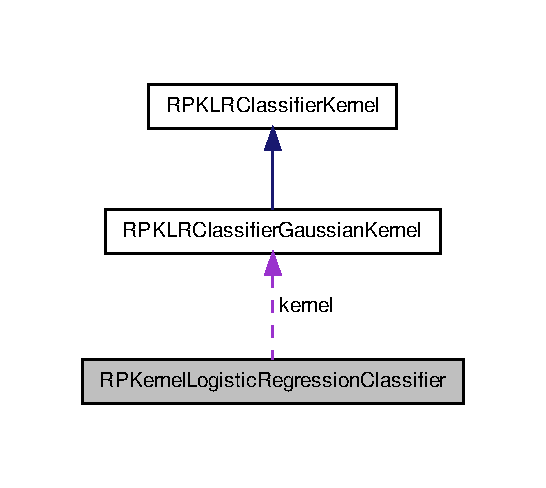
\includegraphics[width=262pt]{class_r_p_kernel_logistic_regression_classifier__coll__graph}
\end{center}
\end{figure}
\subsection*{\-Public \-Member \-Functions}
\begin{DoxyCompactItemize}
\item 
\hyperlink{class_r_p_kernel_logistic_regression_classifier_adfefd03cb8914d0223eab1d874d01966}{\-R\-P\-Kernel\-Logistic\-Regression\-Classifier} ()
\item 
void \hyperlink{class_r_p_kernel_logistic_regression_classifier_a76e06607099d33da606753c347dab738}{add\-Training\-Sample} (std\-::vector$<$ double $>$ \&features, bool is\-\_\-positive)
\item 
void \hyperlink{class_r_p_kernel_logistic_regression_classifier_a1e14b7daeb2fb65768c991b8d8837245}{train} (double time\-\_\-limit\-\_\-s)
\item 
bool \hyperlink{class_r_p_kernel_logistic_regression_classifier_aba1607052f771fe0951842a07b0ab2f4}{classify} (const std\-::vector$<$ double $>$ \&x)
\item 
double \hyperlink{class_r_p_kernel_logistic_regression_classifier_ad0e48344b6b6f4385752e55b51e98f4e}{probability} (const std\-::vector$<$ double $>$ \&x)
\item 
void \hyperlink{class_r_p_kernel_logistic_regression_classifier_a5bed4779fa0d28fca1d06627293d3070}{reset} ()
\end{DoxyCompactItemize}
\subsection*{\-Private \-Member \-Functions}
\begin{DoxyCompactItemize}
\item 
double \hyperlink{class_r_p_kernel_logistic_regression_classifier_aebdb3d0fd4689a5bfbd5cdb14ff6a0bb}{sigmoid} (double z)
\item 
int \hyperlink{class_r_p_kernel_logistic_regression_classifier_a60ad808101bb5de47f531158aa97cd6b}{sgn} (double z)
\item 
double \hyperlink{class_r_p_kernel_logistic_regression_classifier_a705f8e34ac01d78f9e7d5b9f323548ad}{gradient\-Step} ()
\end{DoxyCompactItemize}
\subsection*{\-Private \-Attributes}
\begin{DoxyCompactItemize}
\item 
std\-::vector$<$ \hyperlink{struct_r_p_training_point}{\-R\-P\-Training\-Point} $>$ \hyperlink{class_r_p_kernel_logistic_regression_classifier_acbfcf7c3dc66d0bd1e1b1a11fc05f2b5}{training\-\_\-points}
\item 
std\-::vector$<$ double $>$ \hyperlink{class_r_p_kernel_logistic_regression_classifier_a0c1b9e50db833060a56d2bbeddcaac6b}{weights}
\item 
std\-::vector$<$ double $>$ \hyperlink{class_r_p_kernel_logistic_regression_classifier_a74b5ba4f13e20dbfe86ee0fd972d648a}{gradient}
\item 
std\-::vector$<$ double $>$ \hyperlink{class_r_p_kernel_logistic_regression_classifier_a9da47f0a98cf88d670eb3458c778f50a}{step\-\_\-sizes}
\item 
\hyperlink{class_r_p_k_l_r_classifier_gaussian_kernel}{\-R\-P\-K\-L\-R\-Classifier\-Gaussian\-Kernel} \hyperlink{class_r_p_kernel_logistic_regression_classifier_ae88d931ebd067f4a290913447a493962}{kernel}
\end{DoxyCompactItemize}


\subsection{\-Detailed \-Description}
\-Kernel logistic regression classifier class. 

\begin{DoxyCopyright}{\-Copyright}
\-Manfredas \-Zabarauskas, 2013. \-All rights reserved. \-This project is released under \-C\-C \-B\-Y-\/\-N\-C-\/\-S\-A (\-Creative \-Commons \-Attribution-\/\-Non\-Commercial-\/\-Share\-Alike) license. 
\end{DoxyCopyright}


\-Definition at line 27 of file kernel\-\_\-logistic\-\_\-regression\-\_\-classifier.\-hpp.



\subsection{\-Constructor \& \-Destructor \-Documentation}
\hypertarget{class_r_p_kernel_logistic_regression_classifier_adfefd03cb8914d0223eab1d874d01966}{\index{\-R\-P\-Kernel\-Logistic\-Regression\-Classifier@{\-R\-P\-Kernel\-Logistic\-Regression\-Classifier}!\-R\-P\-Kernel\-Logistic\-Regression\-Classifier@{\-R\-P\-Kernel\-Logistic\-Regression\-Classifier}}
\index{\-R\-P\-Kernel\-Logistic\-Regression\-Classifier@{\-R\-P\-Kernel\-Logistic\-Regression\-Classifier}!RPKernelLogisticRegressionClassifier@{\-R\-P\-Kernel\-Logistic\-Regression\-Classifier}}
\subsubsection[{\-R\-P\-Kernel\-Logistic\-Regression\-Classifier}]{\setlength{\rightskip}{0pt plus 5cm}{\bf \-R\-P\-Kernel\-Logistic\-Regression\-Classifier\-::\-R\-P\-Kernel\-Logistic\-Regression\-Classifier} (
\begin{DoxyParamCaption}
{}
\end{DoxyParamCaption}
)\hspace{0.3cm}{\ttfamily  \mbox{[}inline\mbox{]}}}}\label{class_r_p_kernel_logistic_regression_classifier_adfefd03cb8914d0223eab1d874d01966}
\-Default kernel logistic regression classifier's constructor. 

\-Definition at line 67 of file kernel\-\_\-logistic\-\_\-regression\-\_\-classifier.\-hpp.



\subsection{\-Member \-Function \-Documentation}
\hypertarget{class_r_p_kernel_logistic_regression_classifier_a76e06607099d33da606753c347dab738}{\index{\-R\-P\-Kernel\-Logistic\-Regression\-Classifier@{\-R\-P\-Kernel\-Logistic\-Regression\-Classifier}!add\-Training\-Sample@{add\-Training\-Sample}}
\index{add\-Training\-Sample@{add\-Training\-Sample}!RPKernelLogisticRegressionClassifier@{\-R\-P\-Kernel\-Logistic\-Regression\-Classifier}}
\subsubsection[{add\-Training\-Sample}]{\setlength{\rightskip}{0pt plus 5cm}void {\bf \-R\-P\-Kernel\-Logistic\-Regression\-Classifier\-::add\-Training\-Sample} (
\begin{DoxyParamCaption}
\item[{std\-::vector$<$ double $>$ \&}]{features, }
\item[{bool}]{is\-\_\-positive}
\end{DoxyParamCaption}
)}}\label{class_r_p_kernel_logistic_regression_classifier_a76e06607099d33da606753c347dab738}
\-Adds a training sample. 
\begin{DoxyParams}{\-Parameters}
{\em features} & \-Input training sample. \\
\hline
{\em is\-\_\-positive} & \-Training sample positive/negative flag.\\
\hline
\end{DoxyParams}
\begin{DoxyCopyright}{\-Copyright}
\-Manfredas \-Zabarauskas, 2013. \-All rights reserved. \-This project is released under \-C\-C \-B\-Y-\/\-N\-C-\/\-S\-A (\-Creative \-Commons \-Attribution-\/\-Non\-Commercial-\/\-Share\-Alike) license. 
\end{DoxyCopyright}


\-Definition at line 11 of file kernel\-\_\-logistic\-\_\-regression\-\_\-classifier.\-cpp.

\hypertarget{class_r_p_kernel_logistic_regression_classifier_aba1607052f771fe0951842a07b0ab2f4}{\index{\-R\-P\-Kernel\-Logistic\-Regression\-Classifier@{\-R\-P\-Kernel\-Logistic\-Regression\-Classifier}!classify@{classify}}
\index{classify@{classify}!RPKernelLogisticRegressionClassifier@{\-R\-P\-Kernel\-Logistic\-Regression\-Classifier}}
\subsubsection[{classify}]{\setlength{\rightskip}{0pt plus 5cm}bool {\bf \-R\-P\-Kernel\-Logistic\-Regression\-Classifier\-::classify} (
\begin{DoxyParamCaption}
\item[{const std\-::vector$<$ double $>$ \&}]{x}
\end{DoxyParamCaption}
)}}\label{class_r_p_kernel_logistic_regression_classifier_aba1607052f771fe0951842a07b0ab2f4}
\-Classifies a given input vector as positive/negative. 
\begin{DoxyParams}{\-Parameters}
{\em x} & \-Input vector to be classified. \\
\hline
\end{DoxyParams}
\begin{DoxyReturn}{\-Returns}
\-Classification of a given input (true -\/ positive, false -\/ negative). 
\end{DoxyReturn}


\-Definition at line 25 of file kernel\-\_\-logistic\-\_\-regression\-\_\-classifier.\-cpp.

\hypertarget{class_r_p_kernel_logistic_regression_classifier_a705f8e34ac01d78f9e7d5b9f323548ad}{\index{\-R\-P\-Kernel\-Logistic\-Regression\-Classifier@{\-R\-P\-Kernel\-Logistic\-Regression\-Classifier}!gradient\-Step@{gradient\-Step}}
\index{gradient\-Step@{gradient\-Step}!RPKernelLogisticRegressionClassifier@{\-R\-P\-Kernel\-Logistic\-Regression\-Classifier}}
\subsubsection[{gradient\-Step}]{\setlength{\rightskip}{0pt plus 5cm}double {\bf \-R\-P\-Kernel\-Logistic\-Regression\-Classifier\-::gradient\-Step} (
\begin{DoxyParamCaption}
{}
\end{DoxyParamCaption}
)\hspace{0.3cm}{\ttfamily  \mbox{[}private\mbox{]}}}}\label{class_r_p_kernel_logistic_regression_classifier_a705f8e34ac01d78f9e7d5b9f323548ad}
\-Performs a single gradient training step using an \-R\-Prop variance algorithm. 

\-Definition at line 43 of file kernel\-\_\-logistic\-\_\-regression\-\_\-classifier.\-cpp.

\hypertarget{class_r_p_kernel_logistic_regression_classifier_ad0e48344b6b6f4385752e55b51e98f4e}{\index{\-R\-P\-Kernel\-Logistic\-Regression\-Classifier@{\-R\-P\-Kernel\-Logistic\-Regression\-Classifier}!probability@{probability}}
\index{probability@{probability}!RPKernelLogisticRegressionClassifier@{\-R\-P\-Kernel\-Logistic\-Regression\-Classifier}}
\subsubsection[{probability}]{\setlength{\rightskip}{0pt plus 5cm}double {\bf \-R\-P\-Kernel\-Logistic\-Regression\-Classifier\-::probability} (
\begin{DoxyParamCaption}
\item[{const std\-::vector$<$ double $>$ \&}]{x}
\end{DoxyParamCaption}
)}}\label{class_r_p_kernel_logistic_regression_classifier_ad0e48344b6b6f4385752e55b51e98f4e}
\-Calculates the probability for a given input vector to be positive. 
\begin{DoxyParams}{\-Parameters}
{\em x} & \-Input vector whose probability to be positive needs to be calculated. \\
\hline
\end{DoxyParams}
\begin{DoxyReturn}{\-Returns}
\-Probability that a given input vector is positive. 
\end{DoxyReturn}


\-Definition at line 31 of file kernel\-\_\-logistic\-\_\-regression\-\_\-classifier.\-cpp.

\hypertarget{class_r_p_kernel_logistic_regression_classifier_a5bed4779fa0d28fca1d06627293d3070}{\index{\-R\-P\-Kernel\-Logistic\-Regression\-Classifier@{\-R\-P\-Kernel\-Logistic\-Regression\-Classifier}!reset@{reset}}
\index{reset@{reset}!RPKernelLogisticRegressionClassifier@{\-R\-P\-Kernel\-Logistic\-Regression\-Classifier}}
\subsubsection[{reset}]{\setlength{\rightskip}{0pt plus 5cm}void {\bf \-R\-P\-Kernel\-Logistic\-Regression\-Classifier\-::reset} (
\begin{DoxyParamCaption}
{}
\end{DoxyParamCaption}
)}}\label{class_r_p_kernel_logistic_regression_classifier_a5bed4779fa0d28fca1d06627293d3070}
\-Resets the state of the kernel logistic regression classifier. 

\-Definition at line 110 of file kernel\-\_\-logistic\-\_\-regression\-\_\-classifier.\-cpp.

\hypertarget{class_r_p_kernel_logistic_regression_classifier_a60ad808101bb5de47f531158aa97cd6b}{\index{\-R\-P\-Kernel\-Logistic\-Regression\-Classifier@{\-R\-P\-Kernel\-Logistic\-Regression\-Classifier}!sgn@{sgn}}
\index{sgn@{sgn}!RPKernelLogisticRegressionClassifier@{\-R\-P\-Kernel\-Logistic\-Regression\-Classifier}}
\subsubsection[{sgn}]{\setlength{\rightskip}{0pt plus 5cm}int {\bf \-R\-P\-Kernel\-Logistic\-Regression\-Classifier\-::sgn} (
\begin{DoxyParamCaption}
\item[{double}]{z}
\end{DoxyParamCaption}
)\hspace{0.3cm}{\ttfamily  \mbox{[}inline, private\mbox{]}}}}\label{class_r_p_kernel_logistic_regression_classifier_a60ad808101bb5de47f531158aa97cd6b}
\-Calculates sign function. 
\begin{DoxyParams}{\-Parameters}
{\em z} & \-Input for sign function. \\
\hline
\end{DoxyParams}
\begin{DoxyReturn}{\-Returns}
\-Sign function applied to the input. 
\end{DoxyReturn}


\-Definition at line 53 of file kernel\-\_\-logistic\-\_\-regression\-\_\-classifier.\-hpp.

\hypertarget{class_r_p_kernel_logistic_regression_classifier_aebdb3d0fd4689a5bfbd5cdb14ff6a0bb}{\index{\-R\-P\-Kernel\-Logistic\-Regression\-Classifier@{\-R\-P\-Kernel\-Logistic\-Regression\-Classifier}!sigmoid@{sigmoid}}
\index{sigmoid@{sigmoid}!RPKernelLogisticRegressionClassifier@{\-R\-P\-Kernel\-Logistic\-Regression\-Classifier}}
\subsubsection[{sigmoid}]{\setlength{\rightskip}{0pt plus 5cm}double {\bf \-R\-P\-Kernel\-Logistic\-Regression\-Classifier\-::sigmoid} (
\begin{DoxyParamCaption}
\item[{double}]{z}
\end{DoxyParamCaption}
)\hspace{0.3cm}{\ttfamily  \mbox{[}inline, private\mbox{]}}}}\label{class_r_p_kernel_logistic_regression_classifier_aebdb3d0fd4689a5bfbd5cdb14ff6a0bb}
\-Calculates sigmoid function. 
\begin{DoxyParams}{\-Parameters}
{\em z} & \-Input for sigmoid function. \\
\hline
\end{DoxyParams}
\begin{DoxyReturn}{\-Returns}
\-Sigmoid function applied to the input. 
\end{DoxyReturn}


\-Definition at line 43 of file kernel\-\_\-logistic\-\_\-regression\-\_\-classifier.\-hpp.

\hypertarget{class_r_p_kernel_logistic_regression_classifier_a1e14b7daeb2fb65768c991b8d8837245}{\index{\-R\-P\-Kernel\-Logistic\-Regression\-Classifier@{\-R\-P\-Kernel\-Logistic\-Regression\-Classifier}!train@{train}}
\index{train@{train}!RPKernelLogisticRegressionClassifier@{\-R\-P\-Kernel\-Logistic\-Regression\-Classifier}}
\subsubsection[{train}]{\setlength{\rightskip}{0pt plus 5cm}void {\bf \-R\-P\-Kernel\-Logistic\-Regression\-Classifier\-::train} (
\begin{DoxyParamCaption}
\item[{double}]{time\-\_\-limit\-\_\-s}
\end{DoxyParamCaption}
)}}\label{class_r_p_kernel_logistic_regression_classifier_a1e14b7daeb2fb65768c991b8d8837245}
\-Trains the \-K\-L\-R classifier using an \-R\-Prop variance algorithm for a given period of time. 
\begin{DoxyParams}{\-Parameters}
{\em time\-\_\-limit\-\_\-s} & \-Training time limit in secods. \\
\hline
\end{DoxyParams}


\-Definition at line 96 of file kernel\-\_\-logistic\-\_\-regression\-\_\-classifier.\-cpp.



\subsection{\-Member \-Data \-Documentation}
\hypertarget{class_r_p_kernel_logistic_regression_classifier_a74b5ba4f13e20dbfe86ee0fd972d648a}{\index{\-R\-P\-Kernel\-Logistic\-Regression\-Classifier@{\-R\-P\-Kernel\-Logistic\-Regression\-Classifier}!gradient@{gradient}}
\index{gradient@{gradient}!RPKernelLogisticRegressionClassifier@{\-R\-P\-Kernel\-Logistic\-Regression\-Classifier}}
\subsubsection[{gradient}]{\setlength{\rightskip}{0pt plus 5cm}std\-::vector$<$double$>$ {\bf \-R\-P\-Kernel\-Logistic\-Regression\-Classifier\-::gradient}\hspace{0.3cm}{\ttfamily  \mbox{[}private\mbox{]}}}}\label{class_r_p_kernel_logistic_regression_classifier_a74b5ba4f13e20dbfe86ee0fd972d648a}
\-Current gradient. 

\-Definition at line 33 of file kernel\-\_\-logistic\-\_\-regression\-\_\-classifier.\-hpp.

\hypertarget{class_r_p_kernel_logistic_regression_classifier_ae88d931ebd067f4a290913447a493962}{\index{\-R\-P\-Kernel\-Logistic\-Regression\-Classifier@{\-R\-P\-Kernel\-Logistic\-Regression\-Classifier}!kernel@{kernel}}
\index{kernel@{kernel}!RPKernelLogisticRegressionClassifier@{\-R\-P\-Kernel\-Logistic\-Regression\-Classifier}}
\subsubsection[{kernel}]{\setlength{\rightskip}{0pt plus 5cm}{\bf \-R\-P\-K\-L\-R\-Classifier\-Gaussian\-Kernel} {\bf \-R\-P\-Kernel\-Logistic\-Regression\-Classifier\-::kernel}\hspace{0.3cm}{\ttfamily  \mbox{[}private\mbox{]}}}}\label{class_r_p_kernel_logistic_regression_classifier_ae88d931ebd067f4a290913447a493962}
\-Classifier's kernel function. 

\-Definition at line 36 of file kernel\-\_\-logistic\-\_\-regression\-\_\-classifier.\-hpp.

\hypertarget{class_r_p_kernel_logistic_regression_classifier_a9da47f0a98cf88d670eb3458c778f50a}{\index{\-R\-P\-Kernel\-Logistic\-Regression\-Classifier@{\-R\-P\-Kernel\-Logistic\-Regression\-Classifier}!step\-\_\-sizes@{step\-\_\-sizes}}
\index{step\-\_\-sizes@{step\-\_\-sizes}!RPKernelLogisticRegressionClassifier@{\-R\-P\-Kernel\-Logistic\-Regression\-Classifier}}
\subsubsection[{step\-\_\-sizes}]{\setlength{\rightskip}{0pt plus 5cm}std\-::vector$<$double$>$ {\bf \-R\-P\-Kernel\-Logistic\-Regression\-Classifier\-::step\-\_\-sizes}\hspace{0.3cm}{\ttfamily  \mbox{[}private\mbox{]}}}}\label{class_r_p_kernel_logistic_regression_classifier_a9da47f0a98cf88d670eb3458c778f50a}
\-Current step sizes. 

\-Definition at line 34 of file kernel\-\_\-logistic\-\_\-regression\-\_\-classifier.\-hpp.

\hypertarget{class_r_p_kernel_logistic_regression_classifier_acbfcf7c3dc66d0bd1e1b1a11fc05f2b5}{\index{\-R\-P\-Kernel\-Logistic\-Regression\-Classifier@{\-R\-P\-Kernel\-Logistic\-Regression\-Classifier}!training\-\_\-points@{training\-\_\-points}}
\index{training\-\_\-points@{training\-\_\-points}!RPKernelLogisticRegressionClassifier@{\-R\-P\-Kernel\-Logistic\-Regression\-Classifier}}
\subsubsection[{training\-\_\-points}]{\setlength{\rightskip}{0pt plus 5cm}std\-::vector$<${\bf \-R\-P\-Training\-Point}$>$ {\bf \-R\-P\-Kernel\-Logistic\-Regression\-Classifier\-::training\-\_\-points}\hspace{0.3cm}{\ttfamily  \mbox{[}private\mbox{]}}}}\label{class_r_p_kernel_logistic_regression_classifier_acbfcf7c3dc66d0bd1e1b1a11fc05f2b5}
\-Training points. 

\-Definition at line 30 of file kernel\-\_\-logistic\-\_\-regression\-\_\-classifier.\-hpp.

\hypertarget{class_r_p_kernel_logistic_regression_classifier_a0c1b9e50db833060a56d2bbeddcaac6b}{\index{\-R\-P\-Kernel\-Logistic\-Regression\-Classifier@{\-R\-P\-Kernel\-Logistic\-Regression\-Classifier}!weights@{weights}}
\index{weights@{weights}!RPKernelLogisticRegressionClassifier@{\-R\-P\-Kernel\-Logistic\-Regression\-Classifier}}
\subsubsection[{weights}]{\setlength{\rightskip}{0pt plus 5cm}std\-::vector$<$double$>$ {\bf \-R\-P\-Kernel\-Logistic\-Regression\-Classifier\-::weights}\hspace{0.3cm}{\ttfamily  \mbox{[}private\mbox{]}}}}\label{class_r_p_kernel_logistic_regression_classifier_a0c1b9e50db833060a56d2bbeddcaac6b}
\-Current weights. 

\-Definition at line 32 of file kernel\-\_\-logistic\-\_\-regression\-\_\-classifier.\-hpp.



\-The documentation for this class was generated from the following files\-:\begin{DoxyCompactItemize}
\item 
rp\-\_\-head\-\_\-tracking/include/kernel\-\_\-logistic\-\_\-regression\-\_\-classifier.\-hpp\item 
rp\-\_\-head\-\_\-tracking/src/kernel\-\_\-logistic\-\_\-regression\-\_\-classifier.\-cpp\end{DoxyCompactItemize}

\hypertarget{class_r_p_k_l_r_classifier_gaussian_kernel}{\section{\-R\-P\-K\-L\-R\-Classifier\-Gaussian\-Kernel \-Class \-Reference}
\label{class_r_p_k_l_r_classifier_gaussian_kernel}\index{\-R\-P\-K\-L\-R\-Classifier\-Gaussian\-Kernel@{\-R\-P\-K\-L\-R\-Classifier\-Gaussian\-Kernel}}
}


\-Kernel logistic regression classifier \-Gaussian (radial basis function, \-R\-B\-F) kernel class.  




{\ttfamily \#include $<$kernel\-\_\-logistic\-\_\-regression\-\_\-classifier\-\_\-kernel.\-hpp$>$}



\-Inheritance diagram for \-R\-P\-K\-L\-R\-Classifier\-Gaussian\-Kernel\-:\nopagebreak
\begin{figure}[H]
\begin{center}
\leavevmode
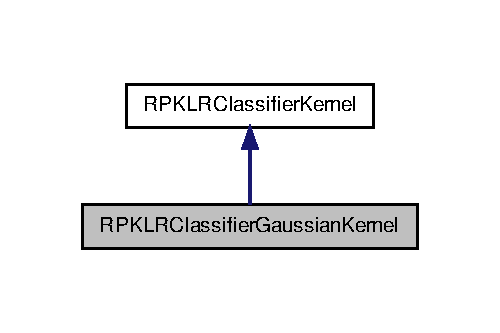
\includegraphics[width=240pt]{class_r_p_k_l_r_classifier_gaussian_kernel__inherit__graph}
\end{center}
\end{figure}


\-Collaboration diagram for \-R\-P\-K\-L\-R\-Classifier\-Gaussian\-Kernel\-:\nopagebreak
\begin{figure}[H]
\begin{center}
\leavevmode
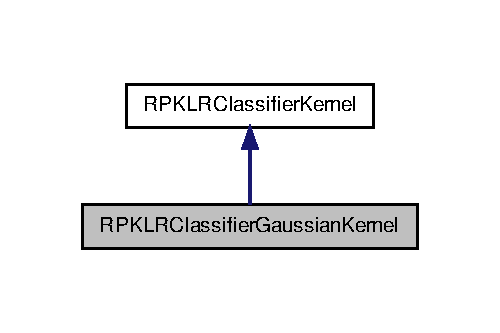
\includegraphics[width=240pt]{class_r_p_k_l_r_classifier_gaussian_kernel__coll__graph}
\end{center}
\end{figure}
\subsection*{\-Public \-Member \-Functions}
\begin{DoxyCompactItemize}
\item 
\hyperlink{class_r_p_k_l_r_classifier_gaussian_kernel_aa2a4bd3a68b3a1ed6f53d56876891006}{\-R\-P\-K\-L\-R\-Classifier\-Gaussian\-Kernel} (double standard\-\_\-deviation)
\item 
virtual double \hyperlink{class_r_p_k_l_r_classifier_gaussian_kernel_aafa64c1a8d66ca122b3e5b2f0fb55acd}{k} (const std\-::vector$<$ double $>$ \&x, const std\-::vector$<$ double $>$ \&y)
\end{DoxyCompactItemize}
\subsection*{\-Private \-Attributes}
\begin{DoxyCompactItemize}
\item 
\hypertarget{class_r_p_k_l_r_classifier_gaussian_kernel_ab03f882cac61547c4c9c4dc71a4f9943}{double {\bfseries standard\-\_\-deviation}}\label{class_r_p_k_l_r_classifier_gaussian_kernel_ab03f882cac61547c4c9c4dc71a4f9943}

\end{DoxyCompactItemize}


\subsection{\-Detailed \-Description}
\-Kernel logistic regression classifier \-Gaussian (radial basis function, \-R\-B\-F) kernel class. 

\-Definition at line 70 of file kernel\-\_\-logistic\-\_\-regression\-\_\-classifier\-\_\-kernel.\-hpp.



\subsection{\-Constructor \& \-Destructor \-Documentation}
\hypertarget{class_r_p_k_l_r_classifier_gaussian_kernel_aa2a4bd3a68b3a1ed6f53d56876891006}{\index{\-R\-P\-K\-L\-R\-Classifier\-Gaussian\-Kernel@{\-R\-P\-K\-L\-R\-Classifier\-Gaussian\-Kernel}!\-R\-P\-K\-L\-R\-Classifier\-Gaussian\-Kernel@{\-R\-P\-K\-L\-R\-Classifier\-Gaussian\-Kernel}}
\index{\-R\-P\-K\-L\-R\-Classifier\-Gaussian\-Kernel@{\-R\-P\-K\-L\-R\-Classifier\-Gaussian\-Kernel}!RPKLRClassifierGaussianKernel@{\-R\-P\-K\-L\-R\-Classifier\-Gaussian\-Kernel}}
\subsubsection[{\-R\-P\-K\-L\-R\-Classifier\-Gaussian\-Kernel}]{\setlength{\rightskip}{0pt plus 5cm}{\bf \-R\-P\-K\-L\-R\-Classifier\-Gaussian\-Kernel\-::\-R\-P\-K\-L\-R\-Classifier\-Gaussian\-Kernel} (
\begin{DoxyParamCaption}
\item[{double}]{standard\-\_\-deviation}
\end{DoxyParamCaption}
)\hspace{0.3cm}{\ttfamily  \mbox{[}inline\mbox{]}}}}\label{class_r_p_k_l_r_classifier_gaussian_kernel_aa2a4bd3a68b3a1ed6f53d56876891006}
\-Constructs a \-Gaussian (\-R\-B\-F) kernel with a given standard deviation. 
\begin{DoxyParams}{\-Parameters}
{\em standard\-\_\-deviation} & \-Standard deviation. \\
\hline
\end{DoxyParams}


\-Definition at line 80 of file kernel\-\_\-logistic\-\_\-regression\-\_\-classifier\-\_\-kernel.\-hpp.



\subsection{\-Member \-Function \-Documentation}
\hypertarget{class_r_p_k_l_r_classifier_gaussian_kernel_aafa64c1a8d66ca122b3e5b2f0fb55acd}{\index{\-R\-P\-K\-L\-R\-Classifier\-Gaussian\-Kernel@{\-R\-P\-K\-L\-R\-Classifier\-Gaussian\-Kernel}!k@{k}}
\index{k@{k}!RPKLRClassifierGaussianKernel@{\-R\-P\-K\-L\-R\-Classifier\-Gaussian\-Kernel}}
\subsubsection[{k}]{\setlength{\rightskip}{0pt plus 5cm}virtual double {\bf \-R\-P\-K\-L\-R\-Classifier\-Gaussian\-Kernel\-::k} (
\begin{DoxyParamCaption}
\item[{const std\-::vector$<$ double $>$ \&}]{x, }
\item[{const std\-::vector$<$ double $>$ \&}]{y}
\end{DoxyParamCaption}
)\hspace{0.3cm}{\ttfamily  \mbox{[}inline, virtual\mbox{]}}}}\label{class_r_p_k_l_r_classifier_gaussian_kernel_aafa64c1a8d66ca122b3e5b2f0fb55acd}
\-Kernel function. 
\begin{DoxyParams}{\-Parameters}
{\em x} & \-First input vector. \\
\hline
{\em y} & \-Second input vector. \\
\hline
\end{DoxyParams}
\begin{DoxyReturn}{\-Returns}
\-Kernel function application result. 
\end{DoxyReturn}


\-Implements \hyperlink{class_r_p_k_l_r_classifier_kernel_a39824eec9f922dc01f151632b2f05649}{\-R\-P\-K\-L\-R\-Classifier\-Kernel}.



\-Definition at line 82 of file kernel\-\_\-logistic\-\_\-regression\-\_\-classifier\-\_\-kernel.\-hpp.



\-The documentation for this class was generated from the following file\-:\begin{DoxyCompactItemize}
\item 
rp\-\_\-head\-\_\-tracking/include/kernel\-\_\-logistic\-\_\-regression\-\_\-classifier\-\_\-kernel.\-hpp\end{DoxyCompactItemize}

\hypertarget{class_r_p_k_l_r_classifier_kernel}{\section{\-R\-P\-K\-L\-R\-Classifier\-Kernel \-Class \-Reference}
\label{class_r_p_k_l_r_classifier_kernel}\index{\-R\-P\-K\-L\-R\-Classifier\-Kernel@{\-R\-P\-K\-L\-R\-Classifier\-Kernel}}
}


\-Kernel logistic regression classifier kernel class.  




{\ttfamily \#include $<$kernel\-\_\-logistic\-\_\-regression\-\_\-classifier\-\_\-kernel.\-hpp$>$}



\-Inheritance diagram for \-R\-P\-K\-L\-R\-Classifier\-Kernel\-:\nopagebreak
\begin{figure}[H]
\begin{center}
\leavevmode
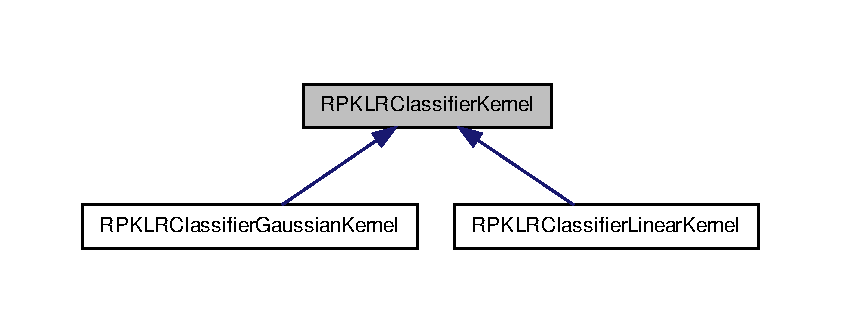
\includegraphics[width=350pt]{class_r_p_k_l_r_classifier_kernel__inherit__graph}
\end{center}
\end{figure}
\subsection*{\-Public \-Member \-Functions}
\begin{DoxyCompactItemize}
\item 
virtual \hyperlink{class_r_p_k_l_r_classifier_kernel_aae696fbcc7a2f9120192ba643c269da9}{$\sim$\-R\-P\-K\-L\-R\-Classifier\-Kernel} ()
\item 
virtual double \hyperlink{class_r_p_k_l_r_classifier_kernel_a39824eec9f922dc01f151632b2f05649}{k} (const std\-::vector$<$ double $>$ \&x, const std\-::vector$<$ double $>$ \&y)=0
\item 
void \hyperlink{class_r_p_k_l_r_classifier_kernel_a31c6e4fca7dcec2829cdfa17d4cd28d2}{build\-Kernel\-Matrix} (const std\-::vector$<$ \hyperlink{struct_r_p_training_point}{\-R\-P\-Training\-Point} $>$ \&training\-\_\-points)
\end{DoxyCompactItemize}
\subsection*{\-Public \-Attributes}
\begin{DoxyCompactItemize}
\item 
cv\-::\-Mat \hyperlink{class_r_p_k_l_r_classifier_kernel_a2dd54b76d322971400ffa60acc6c1c23}{kernel\-\_\-matrix}
\end{DoxyCompactItemize}


\subsection{\-Detailed \-Description}
\-Kernel logistic regression classifier kernel class. 

\begin{DoxyCopyright}{\-Copyright}
\-Manfredas \-Zabarauskas, 2013. \-All rights reserved. \-This project is released under \-C\-C \-B\-Y-\/\-N\-C-\/\-S\-A (\-Creative \-Commons \-Attribution-\/\-Non\-Commercial-\/\-Share\-Alike) license. 
\end{DoxyCopyright}


\-Definition at line 21 of file kernel\-\_\-logistic\-\_\-regression\-\_\-classifier\-\_\-kernel.\-hpp.



\subsection{\-Constructor \& \-Destructor \-Documentation}
\hypertarget{class_r_p_k_l_r_classifier_kernel_aae696fbcc7a2f9120192ba643c269da9}{\index{\-R\-P\-K\-L\-R\-Classifier\-Kernel@{\-R\-P\-K\-L\-R\-Classifier\-Kernel}!$\sim$\-R\-P\-K\-L\-R\-Classifier\-Kernel@{$\sim$\-R\-P\-K\-L\-R\-Classifier\-Kernel}}
\index{$\sim$\-R\-P\-K\-L\-R\-Classifier\-Kernel@{$\sim$\-R\-P\-K\-L\-R\-Classifier\-Kernel}!RPKLRClassifierKernel@{\-R\-P\-K\-L\-R\-Classifier\-Kernel}}
\subsubsection[{$\sim$\-R\-P\-K\-L\-R\-Classifier\-Kernel}]{\setlength{\rightskip}{0pt plus 5cm}virtual {\bf \-R\-P\-K\-L\-R\-Classifier\-Kernel\-::$\sim$\-R\-P\-K\-L\-R\-Classifier\-Kernel} (
\begin{DoxyParamCaption}
{}
\end{DoxyParamCaption}
)\hspace{0.3cm}{\ttfamily  \mbox{[}inline, virtual\mbox{]}}}}\label{class_r_p_k_l_r_classifier_kernel_aae696fbcc7a2f9120192ba643c269da9}
\-Default virtual destructor. 

\-Definition at line 29 of file kernel\-\_\-logistic\-\_\-regression\-\_\-classifier\-\_\-kernel.\-hpp.



\subsection{\-Member \-Function \-Documentation}
\hypertarget{class_r_p_k_l_r_classifier_kernel_a31c6e4fca7dcec2829cdfa17d4cd28d2}{\index{\-R\-P\-K\-L\-R\-Classifier\-Kernel@{\-R\-P\-K\-L\-R\-Classifier\-Kernel}!build\-Kernel\-Matrix@{build\-Kernel\-Matrix}}
\index{build\-Kernel\-Matrix@{build\-Kernel\-Matrix}!RPKLRClassifierKernel@{\-R\-P\-K\-L\-R\-Classifier\-Kernel}}
\subsubsection[{build\-Kernel\-Matrix}]{\setlength{\rightskip}{0pt plus 5cm}void {\bf \-R\-P\-K\-L\-R\-Classifier\-Kernel\-::build\-Kernel\-Matrix} (
\begin{DoxyParamCaption}
\item[{const std\-::vector$<$ {\bf \-R\-P\-Training\-Point} $>$ \&}]{training\-\_\-points}
\end{DoxyParamCaption}
)}}\label{class_r_p_k_l_r_classifier_kernel_a31c6e4fca7dcec2829cdfa17d4cd28d2}
\-Builds kernel matrix.  \-List of training points.

\begin{DoxyCopyright}{\-Copyright}
\-Manfredas \-Zabarauskas, 2013. \-All rights reserved. \-This project is released under \-C\-C \-B\-Y-\/\-N\-C-\/\-S\-A (\-Creative \-Commons \-Attribution-\/\-Non\-Commercial-\/\-Share\-Alike) license. 
\end{DoxyCopyright}


\-Definition at line 7 of file kernel\-\_\-logistic\-\_\-regression\-\_\-classifier\-\_\-kernel.\-cpp.

\hypertarget{class_r_p_k_l_r_classifier_kernel_a39824eec9f922dc01f151632b2f05649}{\index{\-R\-P\-K\-L\-R\-Classifier\-Kernel@{\-R\-P\-K\-L\-R\-Classifier\-Kernel}!k@{k}}
\index{k@{k}!RPKLRClassifierKernel@{\-R\-P\-K\-L\-R\-Classifier\-Kernel}}
\subsubsection[{k}]{\setlength{\rightskip}{0pt plus 5cm}virtual double {\bf \-R\-P\-K\-L\-R\-Classifier\-Kernel\-::k} (
\begin{DoxyParamCaption}
\item[{const std\-::vector$<$ double $>$ \&}]{x, }
\item[{const std\-::vector$<$ double $>$ \&}]{y}
\end{DoxyParamCaption}
)\hspace{0.3cm}{\ttfamily  \mbox{[}pure virtual\mbox{]}}}}\label{class_r_p_k_l_r_classifier_kernel_a39824eec9f922dc01f151632b2f05649}
\-Kernel function. 
\begin{DoxyParams}{\-Parameters}
{\em x} & \-First input vector. \\
\hline
{\em y} & \-Second input vector. \\
\hline
\end{DoxyParams}
\begin{DoxyReturn}{\-Returns}
\-Kernel function application result. 
\end{DoxyReturn}


\-Implemented in \hyperlink{class_r_p_k_l_r_classifier_gaussian_kernel_aafa64c1a8d66ca122b3e5b2f0fb55acd}{\-R\-P\-K\-L\-R\-Classifier\-Gaussian\-Kernel}, and \hyperlink{class_r_p_k_l_r_classifier_linear_kernel_a14bf5a0a448313c76b88aa7d2e7ea1f3}{\-R\-P\-K\-L\-R\-Classifier\-Linear\-Kernel}.



\subsection{\-Member \-Data \-Documentation}
\hypertarget{class_r_p_k_l_r_classifier_kernel_a2dd54b76d322971400ffa60acc6c1c23}{\index{\-R\-P\-K\-L\-R\-Classifier\-Kernel@{\-R\-P\-K\-L\-R\-Classifier\-Kernel}!kernel\-\_\-matrix@{kernel\-\_\-matrix}}
\index{kernel\-\_\-matrix@{kernel\-\_\-matrix}!RPKLRClassifierKernel@{\-R\-P\-K\-L\-R\-Classifier\-Kernel}}
\subsubsection[{kernel\-\_\-matrix}]{\setlength{\rightskip}{0pt plus 5cm}cv\-::\-Mat {\bf \-R\-P\-K\-L\-R\-Classifier\-Kernel\-::kernel\-\_\-matrix}}}\label{class_r_p_k_l_r_classifier_kernel_a2dd54b76d322971400ffa60acc6c1c23}
\-Kernel matrix. 

\-Definition at line 24 of file kernel\-\_\-logistic\-\_\-regression\-\_\-classifier\-\_\-kernel.\-hpp.



\-The documentation for this class was generated from the following files\-:\begin{DoxyCompactItemize}
\item 
rp\-\_\-head\-\_\-tracking/include/kernel\-\_\-logistic\-\_\-regression\-\_\-classifier\-\_\-kernel.\-hpp\item 
rp\-\_\-head\-\_\-tracking/src/kernel\-\_\-logistic\-\_\-regression\-\_\-classifier\-\_\-kernel.\-cpp\end{DoxyCompactItemize}

\hypertarget{class_r_p_k_l_r_classifier_linear_kernel}{\section{\-R\-P\-K\-L\-R\-Classifier\-Linear\-Kernel \-Class \-Reference}
\label{class_r_p_k_l_r_classifier_linear_kernel}\index{\-R\-P\-K\-L\-R\-Classifier\-Linear\-Kernel@{\-R\-P\-K\-L\-R\-Classifier\-Linear\-Kernel}}
}


\-Kernel logistic regression classifier linear kernel class.  




{\ttfamily \#include $<$kernel\-\_\-logistic\-\_\-regression\-\_\-classifier\-\_\-kernel.\-hpp$>$}



\-Inheritance diagram for \-R\-P\-K\-L\-R\-Classifier\-Linear\-Kernel\-:\nopagebreak
\begin{figure}[H]
\begin{center}
\leavevmode
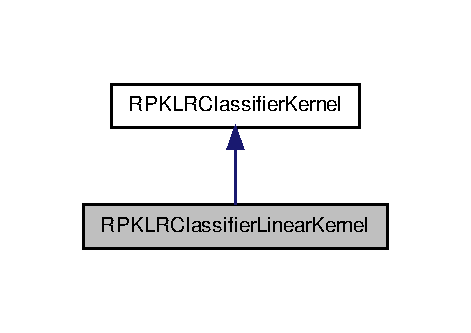
\includegraphics[width=226pt]{class_r_p_k_l_r_classifier_linear_kernel__inherit__graph}
\end{center}
\end{figure}


\-Collaboration diagram for \-R\-P\-K\-L\-R\-Classifier\-Linear\-Kernel\-:\nopagebreak
\begin{figure}[H]
\begin{center}
\leavevmode
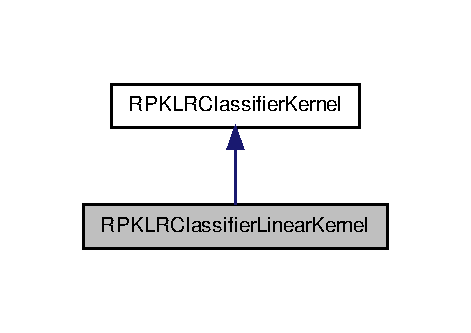
\includegraphics[width=226pt]{class_r_p_k_l_r_classifier_linear_kernel__coll__graph}
\end{center}
\end{figure}
\subsection*{\-Public \-Member \-Functions}
\begin{DoxyCompactItemize}
\item 
virtual double \hyperlink{class_r_p_k_l_r_classifier_linear_kernel_a14bf5a0a448313c76b88aa7d2e7ea1f3}{k} (const std\-::vector$<$ double $>$ \&x, const std\-::vector$<$ double $>$ \&y)
\end{DoxyCompactItemize}


\subsection{\-Detailed \-Description}
\-Kernel logistic regression classifier linear kernel class. 

\-Definition at line 50 of file kernel\-\_\-logistic\-\_\-regression\-\_\-classifier\-\_\-kernel.\-hpp.



\subsection{\-Member \-Function \-Documentation}
\hypertarget{class_r_p_k_l_r_classifier_linear_kernel_a14bf5a0a448313c76b88aa7d2e7ea1f3}{\index{\-R\-P\-K\-L\-R\-Classifier\-Linear\-Kernel@{\-R\-P\-K\-L\-R\-Classifier\-Linear\-Kernel}!k@{k}}
\index{k@{k}!RPKLRClassifierLinearKernel@{\-R\-P\-K\-L\-R\-Classifier\-Linear\-Kernel}}
\subsubsection[{k}]{\setlength{\rightskip}{0pt plus 5cm}virtual double {\bf \-R\-P\-K\-L\-R\-Classifier\-Linear\-Kernel\-::k} (
\begin{DoxyParamCaption}
\item[{const std\-::vector$<$ double $>$ \&}]{x, }
\item[{const std\-::vector$<$ double $>$ \&}]{y}
\end{DoxyParamCaption}
)\hspace{0.3cm}{\ttfamily  \mbox{[}inline, virtual\mbox{]}}}}\label{class_r_p_k_l_r_classifier_linear_kernel_a14bf5a0a448313c76b88aa7d2e7ea1f3}
\-Kernel function. 
\begin{DoxyParams}{\-Parameters}
{\em x} & \-First input vector. \\
\hline
{\em y} & \-Second input vector. \\
\hline
\end{DoxyParams}
\begin{DoxyReturn}{\-Returns}
\-Kernel function application result. 
\end{DoxyReturn}


\-Implements \hyperlink{class_r_p_k_l_r_classifier_kernel_a39824eec9f922dc01f151632b2f05649}{\-R\-P\-K\-L\-R\-Classifier\-Kernel}.



\-Definition at line 53 of file kernel\-\_\-logistic\-\_\-regression\-\_\-classifier\-\_\-kernel.\-hpp.



\-The documentation for this class was generated from the following file\-:\begin{DoxyCompactItemize}
\item 
rp\-\_\-head\-\_\-tracking/include/kernel\-\_\-logistic\-\_\-regression\-\_\-classifier\-\_\-kernel.\-hpp\end{DoxyCompactItemize}

\hypertarget{class_r_p_locomotion_node}{\section{\-R\-P\-Locomotion\-Node \-Class \-Reference}
\label{class_r_p_locomotion_node}\index{\-R\-P\-Locomotion\-Node@{\-R\-P\-Locomotion\-Node}}
}


\-Robot photographer's locomotion node, which converts driving direction messages and bumper press events into linear/angular velocity messages.  




{\ttfamily \#include $<$locomotion.\-hpp$>$}

\subsection*{\-Public \-Member \-Functions}
\begin{DoxyCompactItemize}
\item 
\hyperlink{class_r_p_locomotion_node_aec52b5a922fa41093d3b976123324134}{\-R\-P\-Locomotion\-Node} (ros\-::\-Node\-Handle \&\hyperlink{class_r_p_locomotion_node_ad07de383fa61683b6dd9c38944e4d33b}{node})
\end{DoxyCompactItemize}
\subsection*{\-Private \-Member \-Functions}
\begin{DoxyCompactItemize}
\item 
void \hyperlink{class_r_p_locomotion_node_ae7b34004f4380cd69c005c880236e673}{clear\-Locomotion\-Message} ()
\item 
void \hyperlink{class_r_p_locomotion_node_a8dc03e77588c06484dbd5de534c0691a}{motors\-Enabled} (bool enabled)
\item 
void \hyperlink{class_r_p_locomotion_node_a7cae2e18baf2774457f81a6e103f8def}{set\-Processing\-Bumper\-Event} (bool processing)
\item 
void \hyperlink{class_r_p_locomotion_node_af2b3ece580cb48b4195709a33bbca9ef}{navigation\-Message\-Callback} (const std\-\_\-msgs\-::\-U\-Int16 \&direction\-\_\-and\-\_\-source\-\_\-code)
\item 
void \hyperlink{class_r_p_locomotion_node_ac82f2e8ea6dab4fa288293c0c51df671}{bumper\-Event\-Callback} (const kobuki\-\_\-msgs\-::\-Bumper\-Event\-Const\-Ptr bumper\-\_\-event)
\item 
void \hyperlink{class_r_p_locomotion_node_aca1892fd551a02799b4e60b8d82a0118}{bumper\-Timer\-Callback} (const ros\-::\-Wall\-Timer\-Event \&timer\-\_\-event)
\item 
void \hyperlink{class_r_p_locomotion_node_ac4ebecd8de7386c96aba8aebb15c3461}{get\-Overridable\-Parameters} ()
\end{DoxyCompactItemize}
\subsection*{\-Private \-Attributes}
\begin{DoxyCompactItemize}
\item 
ros\-::\-Node\-Handle \& \hyperlink{class_r_p_locomotion_node_ad07de383fa61683b6dd9c38944e4d33b}{node}
\item 
geometry\-\_\-msgs\-::\-Twist\-Ptr \hyperlink{class_r_p_locomotion_node_ac9668ec315e5c8b9b45e6c1ee9cd18ee}{locomotion\-\_\-message}
\item 
boost\-::mutex \hyperlink{class_r_p_locomotion_node_aa852cb0599e4ad545d01339479d20121}{locomotion\-\_\-message\-\_\-mutex}
\item 
ros\-::\-Publisher \hyperlink{class_r_p_locomotion_node_a1dca36a6b277f383b193f06c52936c08}{locomotion\-\_\-publisher}
\item 
ros\-::\-Publisher \hyperlink{class_r_p_locomotion_node_aceea8151b1de15fbf9485e1f301db004}{state\-\_\-publisher}
\item 
ros\-::\-Publisher \hyperlink{class_r_p_locomotion_node_a89e8536163d4d7b1f2c10f27dbb16724}{motor\-\_\-power\-\_\-publisher}
\item 
ros\-::\-Subscriber \hyperlink{class_r_p_locomotion_node_a653bdeea59dab13aa8b207ed726b055c}{navigation\-\_\-subscriber}
\item 
ros\-::\-Subscriber \hyperlink{class_r_p_locomotion_node_a7b70ee96f05b97044e14b81c383c671e}{bumper\-\_\-subscriber}
\item 
ros\-::\-Subscriber \hyperlink{class_r_p_locomotion_node_a90e0e6121d6eddacb4c7a4598f29b331}{cnc\-\_\-subscriber}
\item 
ros\-::\-Wall\-Timer \hyperlink{class_r_p_locomotion_node_ae8be6c08928b529659031829fb1f9d31}{bumper\-\_\-timer}
\item 
volatile bool \hyperlink{class_r_p_locomotion_node_acf41adc43410bff9116a493b42ffde87}{processing\-\_\-bumper\-\_\-event}
\item 
double \hyperlink{class_r_p_locomotion_node_a35b3c79ea9c02d5a8d7c01148187a95f}{\-F\-R\-A\-M\-I\-N\-G\-\_\-\-L\-I\-N\-E\-A\-R\-\_\-\-V\-E\-L\-O\-C\-I\-T\-Y}
\item 
double \hyperlink{class_r_p_locomotion_node_aeed6c095a09f0e720615d21c247a7091}{\-F\-R\-A\-M\-I\-N\-G\-\_\-\-A\-N\-G\-U\-L\-A\-R\-\_\-\-V\-E\-L\-O\-C\-I\-T\-Y}
\item 
double \hyperlink{class_r_p_locomotion_node_acfdd2fb267d49557666d59d640f83bdd}{\-O\-B\-S\-T\-A\-C\-L\-E\-\_\-\-A\-V\-O\-I\-D\-A\-N\-C\-E\-\_\-\-L\-I\-N\-E\-A\-R\-\_\-\-V\-E\-L\-O\-C\-I\-T\-Y}
\item 
double \hyperlink{class_r_p_locomotion_node_abbdfb4df3d7f36c1931d48d49a5ffc30}{\-O\-B\-S\-T\-A\-C\-L\-E\-\_\-\-A\-V\-O\-I\-D\-A\-N\-C\-E\-\_\-\-A\-N\-G\-U\-L\-A\-R\-\_\-\-V\-E\-L\-O\-C\-I\-T\-Y}
\end{DoxyCompactItemize}


\subsection{\-Detailed \-Description}
\-Robot photographer's locomotion node, which converts driving direction messages and bumper press events into linear/angular velocity messages. 

\begin{DoxyCopyright}{\-Copyright}
\-Manfredas \-Zabarauskas, 2013. \-All rights reserved. \-This project is released under \-C\-C \-B\-Y-\/\-N\-C-\/\-S\-A (\-Creative \-Commons \-Attribution-\/\-Non\-Commercial-\/\-Share\-Alike) license. 
\end{DoxyCopyright}


\-Definition at line 33 of file locomotion.\-hpp.



\subsection{\-Constructor \& \-Destructor \-Documentation}
\hypertarget{class_r_p_locomotion_node_aec52b5a922fa41093d3b976123324134}{\index{\-R\-P\-Locomotion\-Node@{\-R\-P\-Locomotion\-Node}!\-R\-P\-Locomotion\-Node@{\-R\-P\-Locomotion\-Node}}
\index{\-R\-P\-Locomotion\-Node@{\-R\-P\-Locomotion\-Node}!RPLocomotionNode@{\-R\-P\-Locomotion\-Node}}
\subsubsection[{\-R\-P\-Locomotion\-Node}]{\setlength{\rightskip}{0pt plus 5cm}{\bf \-R\-P\-Locomotion\-Node\-::\-R\-P\-Locomotion\-Node} (
\begin{DoxyParamCaption}
\item[{ros\-::\-Node\-Handle \&}]{node}
\end{DoxyParamCaption}
)}}\label{class_r_p_locomotion_node_aec52b5a922fa41093d3b976123324134}
\-Default locomotion node's constructor. 
\begin{DoxyParams}{\-Parameters}
{\em node} & \-Handle to \-R\-O\-S node. \\
\hline
\end{DoxyParams}


\-Definition at line 30 of file locomotion.\-cpp.



\subsection{\-Member \-Function \-Documentation}
\hypertarget{class_r_p_locomotion_node_ac82f2e8ea6dab4fa288293c0c51df671}{\index{\-R\-P\-Locomotion\-Node@{\-R\-P\-Locomotion\-Node}!bumper\-Event\-Callback@{bumper\-Event\-Callback}}
\index{bumper\-Event\-Callback@{bumper\-Event\-Callback}!RPLocomotionNode@{\-R\-P\-Locomotion\-Node}}
\subsubsection[{bumper\-Event\-Callback}]{\setlength{\rightskip}{0pt plus 5cm}void {\bf \-R\-P\-Locomotion\-Node\-::bumper\-Event\-Callback} (
\begin{DoxyParamCaption}
\item[{const kobuki\-\_\-msgs\-::\-Bumper\-Event\-Const\-Ptr}]{bumper\-\_\-event}
\end{DoxyParamCaption}
)\hspace{0.3cm}{\ttfamily  \mbox{[}private\mbox{]}}}}\label{class_r_p_locomotion_node_ac82f2e8ea6dab4fa288293c0c51df671}
\-Callback for the received bumper event. 
\begin{DoxyParams}{\-Parameters}
{\em timer\-\_\-event} & \-Pointer to the bumper event object. \\
\hline
\end{DoxyParams}


\-Definition at line 99 of file locomotion.\-cpp.

\hypertarget{class_r_p_locomotion_node_aca1892fd551a02799b4e60b8d82a0118}{\index{\-R\-P\-Locomotion\-Node@{\-R\-P\-Locomotion\-Node}!bumper\-Timer\-Callback@{bumper\-Timer\-Callback}}
\index{bumper\-Timer\-Callback@{bumper\-Timer\-Callback}!RPLocomotionNode@{\-R\-P\-Locomotion\-Node}}
\subsubsection[{bumper\-Timer\-Callback}]{\setlength{\rightskip}{0pt plus 5cm}void {\bf \-R\-P\-Locomotion\-Node\-::bumper\-Timer\-Callback} (
\begin{DoxyParamCaption}
\item[{const ros\-::\-Wall\-Timer\-Event \&}]{timer\-\_\-event}
\end{DoxyParamCaption}
)\hspace{0.3cm}{\ttfamily  \mbox{[}private\mbox{]}}}}\label{class_r_p_locomotion_node_aca1892fd551a02799b4e60b8d82a0118}
\-Callback for the bumper timer event. 
\begin{DoxyParams}{\-Parameters}
{\em timer\-\_\-event} & \-Timer callback object. \\
\hline
\end{DoxyParams}


\-Definition at line 91 of file locomotion.\-cpp.

\hypertarget{class_r_p_locomotion_node_ae7b34004f4380cd69c005c880236e673}{\index{\-R\-P\-Locomotion\-Node@{\-R\-P\-Locomotion\-Node}!clear\-Locomotion\-Message@{clear\-Locomotion\-Message}}
\index{clear\-Locomotion\-Message@{clear\-Locomotion\-Message}!RPLocomotionNode@{\-R\-P\-Locomotion\-Node}}
\subsubsection[{clear\-Locomotion\-Message}]{\setlength{\rightskip}{0pt plus 5cm}void {\bf \-R\-P\-Locomotion\-Node\-::clear\-Locomotion\-Message} (
\begin{DoxyParamCaption}
{}
\end{DoxyParamCaption}
)\hspace{0.3cm}{\ttfamily  \mbox{[}private\mbox{]}}}}\label{class_r_p_locomotion_node_ae7b34004f4380cd69c005c880236e673}
\-Resets the locomotion message to stop the robot. 
\begin{DoxyParams}{\-Parameters}
{\em frame\-\_\-message} & \-Input framing status message. \\
\hline
\end{DoxyParams}


\-Definition at line 213 of file locomotion.\-cpp.

\hypertarget{class_r_p_locomotion_node_ac4ebecd8de7386c96aba8aebb15c3461}{\index{\-R\-P\-Locomotion\-Node@{\-R\-P\-Locomotion\-Node}!get\-Overridable\-Parameters@{get\-Overridable\-Parameters}}
\index{get\-Overridable\-Parameters@{get\-Overridable\-Parameters}!RPLocomotionNode@{\-R\-P\-Locomotion\-Node}}
\subsubsection[{get\-Overridable\-Parameters}]{\setlength{\rightskip}{0pt plus 5cm}void {\bf \-R\-P\-Locomotion\-Node\-::get\-Overridable\-Parameters} (
\begin{DoxyParamCaption}
{}
\end{DoxyParamCaption}
)\hspace{0.3cm}{\ttfamily  \mbox{[}private\mbox{]}}}}\label{class_r_p_locomotion_node_ac4ebecd8de7386c96aba8aebb15c3461}
\-Gets the overridable parameters from the parameter server. 

\-Definition at line 71 of file locomotion.\-cpp.

\hypertarget{class_r_p_locomotion_node_a8dc03e77588c06484dbd5de534c0691a}{\index{\-R\-P\-Locomotion\-Node@{\-R\-P\-Locomotion\-Node}!motors\-Enabled@{motors\-Enabled}}
\index{motors\-Enabled@{motors\-Enabled}!RPLocomotionNode@{\-R\-P\-Locomotion\-Node}}
\subsubsection[{motors\-Enabled}]{\setlength{\rightskip}{0pt plus 5cm}void {\bf \-R\-P\-Locomotion\-Node\-::motors\-Enabled} (
\begin{DoxyParamCaption}
\item[{bool}]{enabled}
\end{DoxyParamCaption}
)\hspace{0.3cm}{\ttfamily  \mbox{[}private\mbox{]}}}}\label{class_r_p_locomotion_node_a8dc03e77588c06484dbd5de534c0691a}
\-Sets the motor enabled state. 
\begin{DoxyParams}{\-Parameters}
{\em enabled} & \-Desired motors state (enabled/disabled). \\
\hline
\end{DoxyParams}


\-Definition at line 224 of file locomotion.\-cpp.

\hypertarget{class_r_p_locomotion_node_af2b3ece580cb48b4195709a33bbca9ef}{\index{\-R\-P\-Locomotion\-Node@{\-R\-P\-Locomotion\-Node}!navigation\-Message\-Callback@{navigation\-Message\-Callback}}
\index{navigation\-Message\-Callback@{navigation\-Message\-Callback}!RPLocomotionNode@{\-R\-P\-Locomotion\-Node}}
\subsubsection[{navigation\-Message\-Callback}]{\setlength{\rightskip}{0pt plus 5cm}void {\bf \-R\-P\-Locomotion\-Node\-::navigation\-Message\-Callback} (
\begin{DoxyParamCaption}
\item[{const std\-\_\-msgs\-::\-U\-Int16 \&}]{direction\-\_\-and\-\_\-source\-\_\-code}
\end{DoxyParamCaption}
)\hspace{0.3cm}{\ttfamily  \mbox{[}private\mbox{]}}}}\label{class_r_p_locomotion_node_af2b3ece580cb48b4195709a33bbca9ef}
\-Callback for the received navigation message. 
\begin{DoxyParams}{\-Parameters}
{\em direction\-\_\-and\-\_\-source\-\_\-code} & \-Driving direction and direction source message. \\
\hline
\end{DoxyParams}


\-Definition at line 144 of file locomotion.\-cpp.

\hypertarget{class_r_p_locomotion_node_a7cae2e18baf2774457f81a6e103f8def}{\index{\-R\-P\-Locomotion\-Node@{\-R\-P\-Locomotion\-Node}!set\-Processing\-Bumper\-Event@{set\-Processing\-Bumper\-Event}}
\index{set\-Processing\-Bumper\-Event@{set\-Processing\-Bumper\-Event}!RPLocomotionNode@{\-R\-P\-Locomotion\-Node}}
\subsubsection[{set\-Processing\-Bumper\-Event}]{\setlength{\rightskip}{0pt plus 5cm}void {\bf \-R\-P\-Locomotion\-Node\-::set\-Processing\-Bumper\-Event} (
\begin{DoxyParamCaption}
\item[{bool}]{processing}
\end{DoxyParamCaption}
)\hspace{0.3cm}{\ttfamily  \mbox{[}private\mbox{]}}}}\label{class_r_p_locomotion_node_a7cae2e18baf2774457f81a6e103f8def}
\-Sets/clears the \char`\"{}processing bumper event\char`\"{} flag. 
\begin{DoxyParams}{\-Parameters}
{\em processing} & \-Desired \char`\"{}processing bumper event\char`\"{} flag. \\
\hline
\end{DoxyParams}


\-Definition at line 80 of file locomotion.\-cpp.



\subsection{\-Member \-Data \-Documentation}
\hypertarget{class_r_p_locomotion_node_a7b70ee96f05b97044e14b81c383c671e}{\index{\-R\-P\-Locomotion\-Node@{\-R\-P\-Locomotion\-Node}!bumper\-\_\-subscriber@{bumper\-\_\-subscriber}}
\index{bumper\-\_\-subscriber@{bumper\-\_\-subscriber}!RPLocomotionNode@{\-R\-P\-Locomotion\-Node}}
\subsubsection[{bumper\-\_\-subscriber}]{\setlength{\rightskip}{0pt plus 5cm}ros\-::\-Subscriber {\bf \-R\-P\-Locomotion\-Node\-::bumper\-\_\-subscriber}\hspace{0.3cm}{\ttfamily  \mbox{[}private\mbox{]}}}}\label{class_r_p_locomotion_node_a7b70ee96f05b97044e14b81c383c671e}
\-Bumper events subscriber. 

\-Definition at line 46 of file locomotion.\-hpp.

\hypertarget{class_r_p_locomotion_node_ae8be6c08928b529659031829fb1f9d31}{\index{\-R\-P\-Locomotion\-Node@{\-R\-P\-Locomotion\-Node}!bumper\-\_\-timer@{bumper\-\_\-timer}}
\index{bumper\-\_\-timer@{bumper\-\_\-timer}!RPLocomotionNode@{\-R\-P\-Locomotion\-Node}}
\subsubsection[{bumper\-\_\-timer}]{\setlength{\rightskip}{0pt plus 5cm}ros\-::\-Wall\-Timer {\bf \-R\-P\-Locomotion\-Node\-::bumper\-\_\-timer}\hspace{0.3cm}{\ttfamily  \mbox{[}private\mbox{]}}}}\label{class_r_p_locomotion_node_ae8be6c08928b529659031829fb1f9d31}
\-Timer for a turn-\/around motion when the bumper event is triggered. 

\-Definition at line 50 of file locomotion.\-hpp.

\hypertarget{class_r_p_locomotion_node_a90e0e6121d6eddacb4c7a4598f29b331}{\index{\-R\-P\-Locomotion\-Node@{\-R\-P\-Locomotion\-Node}!cnc\-\_\-subscriber@{cnc\-\_\-subscriber}}
\index{cnc\-\_\-subscriber@{cnc\-\_\-subscriber}!RPLocomotionNode@{\-R\-P\-Locomotion\-Node}}
\subsubsection[{cnc\-\_\-subscriber}]{\setlength{\rightskip}{0pt plus 5cm}ros\-::\-Subscriber {\bf \-R\-P\-Locomotion\-Node\-::cnc\-\_\-subscriber}\hspace{0.3cm}{\ttfamily  \mbox{[}private\mbox{]}}}}\label{class_r_p_locomotion_node_a90e0e6121d6eddacb4c7a4598f29b331}
\-C\&\-C input subscriber which determines the source of driving direction. 

\-Definition at line 47 of file locomotion.\-hpp.

\hypertarget{class_r_p_locomotion_node_aeed6c095a09f0e720615d21c247a7091}{\index{\-R\-P\-Locomotion\-Node@{\-R\-P\-Locomotion\-Node}!\-F\-R\-A\-M\-I\-N\-G\-\_\-\-A\-N\-G\-U\-L\-A\-R\-\_\-\-V\-E\-L\-O\-C\-I\-T\-Y@{\-F\-R\-A\-M\-I\-N\-G\-\_\-\-A\-N\-G\-U\-L\-A\-R\-\_\-\-V\-E\-L\-O\-C\-I\-T\-Y}}
\index{\-F\-R\-A\-M\-I\-N\-G\-\_\-\-A\-N\-G\-U\-L\-A\-R\-\_\-\-V\-E\-L\-O\-C\-I\-T\-Y@{\-F\-R\-A\-M\-I\-N\-G\-\_\-\-A\-N\-G\-U\-L\-A\-R\-\_\-\-V\-E\-L\-O\-C\-I\-T\-Y}!RPLocomotionNode@{\-R\-P\-Locomotion\-Node}}
\subsubsection[{\-F\-R\-A\-M\-I\-N\-G\-\_\-\-A\-N\-G\-U\-L\-A\-R\-\_\-\-V\-E\-L\-O\-C\-I\-T\-Y}]{\setlength{\rightskip}{0pt plus 5cm}double {\bf \-R\-P\-Locomotion\-Node\-::\-F\-R\-A\-M\-I\-N\-G\-\_\-\-A\-N\-G\-U\-L\-A\-R\-\_\-\-V\-E\-L\-O\-C\-I\-T\-Y}\hspace{0.3cm}{\ttfamily  \mbox{[}private\mbox{]}}}}\label{class_r_p_locomotion_node_aeed6c095a09f0e720615d21c247a7091}
\-Framing angular velocity \-O\-P. 

\-Definition at line 56 of file locomotion.\-hpp.

\hypertarget{class_r_p_locomotion_node_a35b3c79ea9c02d5a8d7c01148187a95f}{\index{\-R\-P\-Locomotion\-Node@{\-R\-P\-Locomotion\-Node}!\-F\-R\-A\-M\-I\-N\-G\-\_\-\-L\-I\-N\-E\-A\-R\-\_\-\-V\-E\-L\-O\-C\-I\-T\-Y@{\-F\-R\-A\-M\-I\-N\-G\-\_\-\-L\-I\-N\-E\-A\-R\-\_\-\-V\-E\-L\-O\-C\-I\-T\-Y}}
\index{\-F\-R\-A\-M\-I\-N\-G\-\_\-\-L\-I\-N\-E\-A\-R\-\_\-\-V\-E\-L\-O\-C\-I\-T\-Y@{\-F\-R\-A\-M\-I\-N\-G\-\_\-\-L\-I\-N\-E\-A\-R\-\_\-\-V\-E\-L\-O\-C\-I\-T\-Y}!RPLocomotionNode@{\-R\-P\-Locomotion\-Node}}
\subsubsection[{\-F\-R\-A\-M\-I\-N\-G\-\_\-\-L\-I\-N\-E\-A\-R\-\_\-\-V\-E\-L\-O\-C\-I\-T\-Y}]{\setlength{\rightskip}{0pt plus 5cm}double {\bf \-R\-P\-Locomotion\-Node\-::\-F\-R\-A\-M\-I\-N\-G\-\_\-\-L\-I\-N\-E\-A\-R\-\_\-\-V\-E\-L\-O\-C\-I\-T\-Y}\hspace{0.3cm}{\ttfamily  \mbox{[}private\mbox{]}}}}\label{class_r_p_locomotion_node_a35b3c79ea9c02d5a8d7c01148187a95f}
\-Framing linear velocity \-O\-P. 

\-Definition at line 55 of file locomotion.\-hpp.

\hypertarget{class_r_p_locomotion_node_ac9668ec315e5c8b9b45e6c1ee9cd18ee}{\index{\-R\-P\-Locomotion\-Node@{\-R\-P\-Locomotion\-Node}!locomotion\-\_\-message@{locomotion\-\_\-message}}
\index{locomotion\-\_\-message@{locomotion\-\_\-message}!RPLocomotionNode@{\-R\-P\-Locomotion\-Node}}
\subsubsection[{locomotion\-\_\-message}]{\setlength{\rightskip}{0pt plus 5cm}geometry\-\_\-msgs\-::\-Twist\-Ptr {\bf \-R\-P\-Locomotion\-Node\-::locomotion\-\_\-message}\hspace{0.3cm}{\ttfamily  \mbox{[}private\mbox{]}}}}\label{class_r_p_locomotion_node_ac9668ec315e5c8b9b45e6c1ee9cd18ee}
\-Pointer to locomotion message. 

\-Definition at line 38 of file locomotion.\-hpp.

\hypertarget{class_r_p_locomotion_node_aa852cb0599e4ad545d01339479d20121}{\index{\-R\-P\-Locomotion\-Node@{\-R\-P\-Locomotion\-Node}!locomotion\-\_\-message\-\_\-mutex@{locomotion\-\_\-message\-\_\-mutex}}
\index{locomotion\-\_\-message\-\_\-mutex@{locomotion\-\_\-message\-\_\-mutex}!RPLocomotionNode@{\-R\-P\-Locomotion\-Node}}
\subsubsection[{locomotion\-\_\-message\-\_\-mutex}]{\setlength{\rightskip}{0pt plus 5cm}boost\-::mutex {\bf \-R\-P\-Locomotion\-Node\-::locomotion\-\_\-message\-\_\-mutex}\hspace{0.3cm}{\ttfamily  \mbox{[}private\mbox{]}}}}\label{class_r_p_locomotion_node_aa852cb0599e4ad545d01339479d20121}
\-Locomotion message's mutex. 

\-Definition at line 39 of file locomotion.\-hpp.

\hypertarget{class_r_p_locomotion_node_a1dca36a6b277f383b193f06c52936c08}{\index{\-R\-P\-Locomotion\-Node@{\-R\-P\-Locomotion\-Node}!locomotion\-\_\-publisher@{locomotion\-\_\-publisher}}
\index{locomotion\-\_\-publisher@{locomotion\-\_\-publisher}!RPLocomotionNode@{\-R\-P\-Locomotion\-Node}}
\subsubsection[{locomotion\-\_\-publisher}]{\setlength{\rightskip}{0pt plus 5cm}ros\-::\-Publisher {\bf \-R\-P\-Locomotion\-Node\-::locomotion\-\_\-publisher}\hspace{0.3cm}{\ttfamily  \mbox{[}private\mbox{]}}}}\label{class_r_p_locomotion_node_a1dca36a6b277f383b193f06c52936c08}
\-Locomotion publisher. 

\-Definition at line 41 of file locomotion.\-hpp.

\hypertarget{class_r_p_locomotion_node_a89e8536163d4d7b1f2c10f27dbb16724}{\index{\-R\-P\-Locomotion\-Node@{\-R\-P\-Locomotion\-Node}!motor\-\_\-power\-\_\-publisher@{motor\-\_\-power\-\_\-publisher}}
\index{motor\-\_\-power\-\_\-publisher@{motor\-\_\-power\-\_\-publisher}!RPLocomotionNode@{\-R\-P\-Locomotion\-Node}}
\subsubsection[{motor\-\_\-power\-\_\-publisher}]{\setlength{\rightskip}{0pt plus 5cm}ros\-::\-Publisher {\bf \-R\-P\-Locomotion\-Node\-::motor\-\_\-power\-\_\-publisher}\hspace{0.3cm}{\ttfamily  \mbox{[}private\mbox{]}}}}\label{class_r_p_locomotion_node_a89e8536163d4d7b1f2c10f27dbb16724}
\-Motor power publisher. 

\-Definition at line 43 of file locomotion.\-hpp.

\hypertarget{class_r_p_locomotion_node_a653bdeea59dab13aa8b207ed726b055c}{\index{\-R\-P\-Locomotion\-Node@{\-R\-P\-Locomotion\-Node}!navigation\-\_\-subscriber@{navigation\-\_\-subscriber}}
\index{navigation\-\_\-subscriber@{navigation\-\_\-subscriber}!RPLocomotionNode@{\-R\-P\-Locomotion\-Node}}
\subsubsection[{navigation\-\_\-subscriber}]{\setlength{\rightskip}{0pt plus 5cm}ros\-::\-Subscriber {\bf \-R\-P\-Locomotion\-Node\-::navigation\-\_\-subscriber}\hspace{0.3cm}{\ttfamily  \mbox{[}private\mbox{]}}}}\label{class_r_p_locomotion_node_a653bdeea59dab13aa8b207ed726b055c}
\-Navigation input subscriber. 

\-Definition at line 45 of file locomotion.\-hpp.

\hypertarget{class_r_p_locomotion_node_ad07de383fa61683b6dd9c38944e4d33b}{\index{\-R\-P\-Locomotion\-Node@{\-R\-P\-Locomotion\-Node}!node@{node}}
\index{node@{node}!RPLocomotionNode@{\-R\-P\-Locomotion\-Node}}
\subsubsection[{node}]{\setlength{\rightskip}{0pt plus 5cm}ros\-::\-Node\-Handle\& {\bf \-R\-P\-Locomotion\-Node\-::node}\hspace{0.3cm}{\ttfamily  \mbox{[}private\mbox{]}}}}\label{class_r_p_locomotion_node_ad07de383fa61683b6dd9c38944e4d33b}
\-Node's handle. 

\-Definition at line 36 of file locomotion.\-hpp.

\hypertarget{class_r_p_locomotion_node_abbdfb4df3d7f36c1931d48d49a5ffc30}{\index{\-R\-P\-Locomotion\-Node@{\-R\-P\-Locomotion\-Node}!\-O\-B\-S\-T\-A\-C\-L\-E\-\_\-\-A\-V\-O\-I\-D\-A\-N\-C\-E\-\_\-\-A\-N\-G\-U\-L\-A\-R\-\_\-\-V\-E\-L\-O\-C\-I\-T\-Y@{\-O\-B\-S\-T\-A\-C\-L\-E\-\_\-\-A\-V\-O\-I\-D\-A\-N\-C\-E\-\_\-\-A\-N\-G\-U\-L\-A\-R\-\_\-\-V\-E\-L\-O\-C\-I\-T\-Y}}
\index{\-O\-B\-S\-T\-A\-C\-L\-E\-\_\-\-A\-V\-O\-I\-D\-A\-N\-C\-E\-\_\-\-A\-N\-G\-U\-L\-A\-R\-\_\-\-V\-E\-L\-O\-C\-I\-T\-Y@{\-O\-B\-S\-T\-A\-C\-L\-E\-\_\-\-A\-V\-O\-I\-D\-A\-N\-C\-E\-\_\-\-A\-N\-G\-U\-L\-A\-R\-\_\-\-V\-E\-L\-O\-C\-I\-T\-Y}!RPLocomotionNode@{\-R\-P\-Locomotion\-Node}}
\subsubsection[{\-O\-B\-S\-T\-A\-C\-L\-E\-\_\-\-A\-V\-O\-I\-D\-A\-N\-C\-E\-\_\-\-A\-N\-G\-U\-L\-A\-R\-\_\-\-V\-E\-L\-O\-C\-I\-T\-Y}]{\setlength{\rightskip}{0pt plus 5cm}double {\bf \-R\-P\-Locomotion\-Node\-::\-O\-B\-S\-T\-A\-C\-L\-E\-\_\-\-A\-V\-O\-I\-D\-A\-N\-C\-E\-\_\-\-A\-N\-G\-U\-L\-A\-R\-\_\-\-V\-E\-L\-O\-C\-I\-T\-Y}\hspace{0.3cm}{\ttfamily  \mbox{[}private\mbox{]}}}}\label{class_r_p_locomotion_node_abbdfb4df3d7f36c1931d48d49a5ffc30}
\-Obstacle avoidance angular velocity \-O\-P. 

\-Definition at line 59 of file locomotion.\-hpp.

\hypertarget{class_r_p_locomotion_node_acfdd2fb267d49557666d59d640f83bdd}{\index{\-R\-P\-Locomotion\-Node@{\-R\-P\-Locomotion\-Node}!\-O\-B\-S\-T\-A\-C\-L\-E\-\_\-\-A\-V\-O\-I\-D\-A\-N\-C\-E\-\_\-\-L\-I\-N\-E\-A\-R\-\_\-\-V\-E\-L\-O\-C\-I\-T\-Y@{\-O\-B\-S\-T\-A\-C\-L\-E\-\_\-\-A\-V\-O\-I\-D\-A\-N\-C\-E\-\_\-\-L\-I\-N\-E\-A\-R\-\_\-\-V\-E\-L\-O\-C\-I\-T\-Y}}
\index{\-O\-B\-S\-T\-A\-C\-L\-E\-\_\-\-A\-V\-O\-I\-D\-A\-N\-C\-E\-\_\-\-L\-I\-N\-E\-A\-R\-\_\-\-V\-E\-L\-O\-C\-I\-T\-Y@{\-O\-B\-S\-T\-A\-C\-L\-E\-\_\-\-A\-V\-O\-I\-D\-A\-N\-C\-E\-\_\-\-L\-I\-N\-E\-A\-R\-\_\-\-V\-E\-L\-O\-C\-I\-T\-Y}!RPLocomotionNode@{\-R\-P\-Locomotion\-Node}}
\subsubsection[{\-O\-B\-S\-T\-A\-C\-L\-E\-\_\-\-A\-V\-O\-I\-D\-A\-N\-C\-E\-\_\-\-L\-I\-N\-E\-A\-R\-\_\-\-V\-E\-L\-O\-C\-I\-T\-Y}]{\setlength{\rightskip}{0pt plus 5cm}double {\bf \-R\-P\-Locomotion\-Node\-::\-O\-B\-S\-T\-A\-C\-L\-E\-\_\-\-A\-V\-O\-I\-D\-A\-N\-C\-E\-\_\-\-L\-I\-N\-E\-A\-R\-\_\-\-V\-E\-L\-O\-C\-I\-T\-Y}\hspace{0.3cm}{\ttfamily  \mbox{[}private\mbox{]}}}}\label{class_r_p_locomotion_node_acfdd2fb267d49557666d59d640f83bdd}
\-Obstacle avoidance linear velocity \-O\-P. 

\-Definition at line 58 of file locomotion.\-hpp.

\hypertarget{class_r_p_locomotion_node_acf41adc43410bff9116a493b42ffde87}{\index{\-R\-P\-Locomotion\-Node@{\-R\-P\-Locomotion\-Node}!processing\-\_\-bumper\-\_\-event@{processing\-\_\-bumper\-\_\-event}}
\index{processing\-\_\-bumper\-\_\-event@{processing\-\_\-bumper\-\_\-event}!RPLocomotionNode@{\-R\-P\-Locomotion\-Node}}
\subsubsection[{processing\-\_\-bumper\-\_\-event}]{\setlength{\rightskip}{0pt plus 5cm}volatile bool {\bf \-R\-P\-Locomotion\-Node\-::processing\-\_\-bumper\-\_\-event}\hspace{0.3cm}{\ttfamily  \mbox{[}private\mbox{]}}}}\label{class_r_p_locomotion_node_acf41adc43410bff9116a493b42ffde87}
\-Bumper event flag. 

\-Definition at line 53 of file locomotion.\-hpp.

\hypertarget{class_r_p_locomotion_node_aceea8151b1de15fbf9485e1f301db004}{\index{\-R\-P\-Locomotion\-Node@{\-R\-P\-Locomotion\-Node}!state\-\_\-publisher@{state\-\_\-publisher}}
\index{state\-\_\-publisher@{state\-\_\-publisher}!RPLocomotionNode@{\-R\-P\-Locomotion\-Node}}
\subsubsection[{state\-\_\-publisher}]{\setlength{\rightskip}{0pt plus 5cm}ros\-::\-Publisher {\bf \-R\-P\-Locomotion\-Node\-::state\-\_\-publisher}\hspace{0.3cm}{\ttfamily  \mbox{[}private\mbox{]}}}}\label{class_r_p_locomotion_node_aceea8151b1de15fbf9485e1f301db004}
\-Locomotion state publisher. 

\-Definition at line 42 of file locomotion.\-hpp.



\-The documentation for this class was generated from the following files\-:\begin{DoxyCompactItemize}
\item 
rp\-\_\-locomotion/include/locomotion.\-hpp\item 
rp\-\_\-locomotion/src/locomotion.\-cpp\end{DoxyCompactItemize}

\hypertarget{class_r_p_mock_head_tracking_node}{\section{\-R\-P\-Mock\-Head\-Tracking\-Node \-Class \-Reference}
\label{class_r_p_mock_head_tracking_node}\index{\-R\-P\-Mock\-Head\-Tracking\-Node@{\-R\-P\-Mock\-Head\-Tracking\-Node}}
}


\-Mock head tracking node that publishes randomly generated head detections, which evolve using a random walk over the scene. \-Useful for framing/composition algorithm testing.  




{\ttfamily \#include $<$mock\-\_\-head\-\_\-tracking.\-hpp$>$}

\subsection*{\-Public \-Member \-Functions}
\begin{DoxyCompactItemize}
\item 
\hyperlink{class_r_p_mock_head_tracking_node_aa4543f859850e3b59dd452b6130cae30}{\-R\-P\-Mock\-Head\-Tracking\-Node} (ros\-::\-Node\-Handle \&\hyperlink{class_r_p_mock_head_tracking_node_a2294de9d2f407990783725f89aca9f43}{node})
\item 
void \hyperlink{class_r_p_mock_head_tracking_node_aba24032613272b902fa46de867036b36}{get\-Overridable\-Parameters} ()
\item 
void \hyperlink{class_r_p_mock_head_tracking_node_aa565b90163780a4a5c8602e006020603}{generate\-And\-Publish\-Mock\-Heads} ()
\item 
void \hyperlink{class_r_p_mock_head_tracking_node_ab9b38d32668df19b25b247ba560f5100}{generate\-Mock\-Head} (cv\-::\-Rect \&generated\-\_\-head)
\item 
void \hyperlink{class_r_p_mock_head_tracking_node_a6da2db9e3d11a3edf49d3ddfe43c2def}{publish\-Heads} ()
\item 
void \hyperlink{class_r_p_mock_head_tracking_node_a0a8464108241e61fdd56c8a92354a8b6}{initialize\-Random\-Depth\-Image} (const cv\-\_\-bridge\-::\-Cv\-Image\-::\-Ptr \&\hyperlink{class_r_p_mock_head_tracking_node_a94d8f99ef984c889f722bc6da057df5f}{depth\-\_\-image})
\end{DoxyCompactItemize}
\subsection*{\-Private \-Attributes}
\begin{DoxyCompactItemize}
\item 
ros\-::\-Node\-Handle \& \hyperlink{class_r_p_mock_head_tracking_node_a2294de9d2f407990783725f89aca9f43}{node}
\item 
unsigned int \hyperlink{class_r_p_mock_head_tracking_node_a00ba80d3ca138d7d586242a5655136f6}{frame\-\_\-count}
\item 
int \hyperlink{class_r_p_mock_head_tracking_node_a7397e364d5dec3ad0068e26dbb50e173}{\-H\-E\-A\-D\-\_\-\-C\-O\-U\-N\-T}
\item 
std\-::vector$<$ \hyperlink{struct_head}{\-Head} $>$ \hyperlink{class_r_p_mock_head_tracking_node_a9eb51fd17b3436f4d4058be0e1a204d8}{heads}
\item 
ros\-::\-Publisher \hyperlink{class_r_p_mock_head_tracking_node_a4d78d8388d295ef1120818d2e8f2954e}{heads\-\_\-publisher}
\item 
cv\-\_\-bridge\-::\-Cv\-Image\-::\-Ptr \hyperlink{class_r_p_mock_head_tracking_node_a94d8f99ef984c889f722bc6da057df5f}{depth\-\_\-image}
\end{DoxyCompactItemize}


\subsection{\-Detailed \-Description}
\-Mock head tracking node that publishes randomly generated head detections, which evolve using a random walk over the scene. \-Useful for framing/composition algorithm testing. 

\begin{DoxyCopyright}{\-Copyright}
\-Manfredas \-Zabarauskas, 2013. \-All rights reserved. \-This project is released under \-C\-C \-B\-Y-\/\-N\-C-\/\-S\-A (\-Creative \-Commons \-Attribution-\/\-Non\-Commercial-\/\-Share\-Alike) license. 
\end{DoxyCopyright}


\-Definition at line 28 of file mock\-\_\-head\-\_\-tracking.\-hpp.



\subsection{\-Constructor \& \-Destructor \-Documentation}
\hypertarget{class_r_p_mock_head_tracking_node_aa4543f859850e3b59dd452b6130cae30}{\index{\-R\-P\-Mock\-Head\-Tracking\-Node@{\-R\-P\-Mock\-Head\-Tracking\-Node}!\-R\-P\-Mock\-Head\-Tracking\-Node@{\-R\-P\-Mock\-Head\-Tracking\-Node}}
\index{\-R\-P\-Mock\-Head\-Tracking\-Node@{\-R\-P\-Mock\-Head\-Tracking\-Node}!RPMockHeadTrackingNode@{\-R\-P\-Mock\-Head\-Tracking\-Node}}
\subsubsection[{\-R\-P\-Mock\-Head\-Tracking\-Node}]{\setlength{\rightskip}{0pt plus 5cm}{\bf \-R\-P\-Mock\-Head\-Tracking\-Node\-::\-R\-P\-Mock\-Head\-Tracking\-Node} (
\begin{DoxyParamCaption}
\item[{ros\-::\-Node\-Handle \&}]{node}
\end{DoxyParamCaption}
)}}\label{class_r_p_mock_head_tracking_node_aa4543f859850e3b59dd452b6130cae30}
\-Default mock head tracking node constructor. 
\begin{DoxyParams}{\-Parameters}
{\em node} & \-Node's handle. \\
\hline
\end{DoxyParams}


\-Definition at line 33 of file mock\-\_\-head\-\_\-tracking.\-cpp.



\subsection{\-Member \-Function \-Documentation}
\hypertarget{class_r_p_mock_head_tracking_node_aa565b90163780a4a5c8602e006020603}{\index{\-R\-P\-Mock\-Head\-Tracking\-Node@{\-R\-P\-Mock\-Head\-Tracking\-Node}!generate\-And\-Publish\-Mock\-Heads@{generate\-And\-Publish\-Mock\-Heads}}
\index{generate\-And\-Publish\-Mock\-Heads@{generate\-And\-Publish\-Mock\-Heads}!RPMockHeadTrackingNode@{\-R\-P\-Mock\-Head\-Tracking\-Node}}
\subsubsection[{generate\-And\-Publish\-Mock\-Heads}]{\setlength{\rightskip}{0pt plus 5cm}void {\bf \-R\-P\-Mock\-Head\-Tracking\-Node\-::generate\-And\-Publish\-Mock\-Heads} (
\begin{DoxyParamCaption}
{}
\end{DoxyParamCaption}
)}}\label{class_r_p_mock_head_tracking_node_aa565b90163780a4a5c8602e006020603}
\-Generates and publishes mock heads. 

\-Definition at line 74 of file mock\-\_\-head\-\_\-tracking.\-cpp.

\hypertarget{class_r_p_mock_head_tracking_node_ab9b38d32668df19b25b247ba560f5100}{\index{\-R\-P\-Mock\-Head\-Tracking\-Node@{\-R\-P\-Mock\-Head\-Tracking\-Node}!generate\-Mock\-Head@{generate\-Mock\-Head}}
\index{generate\-Mock\-Head@{generate\-Mock\-Head}!RPMockHeadTrackingNode@{\-R\-P\-Mock\-Head\-Tracking\-Node}}
\subsubsection[{generate\-Mock\-Head}]{\setlength{\rightskip}{0pt plus 5cm}void {\bf \-R\-P\-Mock\-Head\-Tracking\-Node\-::generate\-Mock\-Head} (
\begin{DoxyParamCaption}
\item[{cv\-::\-Rect \&}]{generated\-\_\-head}
\end{DoxyParamCaption}
)}}\label{class_r_p_mock_head_tracking_node_ab9b38d32668df19b25b247ba560f5100}
\-Generates a single mock head. 
\begin{DoxyParams}{\-Parameters}
{\em generated\-\_\-head} & \-Resulting generated mock head rectangle. \\
\hline
\end{DoxyParams}


\-Definition at line 136 of file mock\-\_\-head\-\_\-tracking.\-cpp.

\hypertarget{class_r_p_mock_head_tracking_node_aba24032613272b902fa46de867036b36}{\index{\-R\-P\-Mock\-Head\-Tracking\-Node@{\-R\-P\-Mock\-Head\-Tracking\-Node}!get\-Overridable\-Parameters@{get\-Overridable\-Parameters}}
\index{get\-Overridable\-Parameters@{get\-Overridable\-Parameters}!RPMockHeadTrackingNode@{\-R\-P\-Mock\-Head\-Tracking\-Node}}
\subsubsection[{get\-Overridable\-Parameters}]{\setlength{\rightskip}{0pt plus 5cm}void {\bf \-R\-P\-Mock\-Head\-Tracking\-Node\-::get\-Overridable\-Parameters} (
\begin{DoxyParamCaption}
{}
\end{DoxyParamCaption}
)}}\label{class_r_p_mock_head_tracking_node_aba24032613272b902fa46de867036b36}
\-Gets overridable parameters from the parameter server. 

\-Definition at line 154 of file mock\-\_\-head\-\_\-tracking.\-cpp.

\hypertarget{class_r_p_mock_head_tracking_node_a0a8464108241e61fdd56c8a92354a8b6}{\index{\-R\-P\-Mock\-Head\-Tracking\-Node@{\-R\-P\-Mock\-Head\-Tracking\-Node}!initialize\-Random\-Depth\-Image@{initialize\-Random\-Depth\-Image}}
\index{initialize\-Random\-Depth\-Image@{initialize\-Random\-Depth\-Image}!RPMockHeadTrackingNode@{\-R\-P\-Mock\-Head\-Tracking\-Node}}
\subsubsection[{initialize\-Random\-Depth\-Image}]{\setlength{\rightskip}{0pt plus 5cm}void {\bf \-R\-P\-Mock\-Head\-Tracking\-Node\-::initialize\-Random\-Depth\-Image} (
\begin{DoxyParamCaption}
\item[{const cv\-\_\-bridge\-::\-Cv\-Image\-::\-Ptr \&}]{depth\-\_\-image}
\end{DoxyParamCaption}
)}}\label{class_r_p_mock_head_tracking_node_a0a8464108241e61fdd56c8a92354a8b6}
\-Initializes a random depth image. 
\begin{DoxyParams}{\-Parameters}
{\em depth\-\_\-image} & \-Generated random depth image. \\
\hline
\end{DoxyParams}


\-Definition at line 56 of file mock\-\_\-head\-\_\-tracking.\-cpp.

\hypertarget{class_r_p_mock_head_tracking_node_a6da2db9e3d11a3edf49d3ddfe43c2def}{\index{\-R\-P\-Mock\-Head\-Tracking\-Node@{\-R\-P\-Mock\-Head\-Tracking\-Node}!publish\-Heads@{publish\-Heads}}
\index{publish\-Heads@{publish\-Heads}!RPMockHeadTrackingNode@{\-R\-P\-Mock\-Head\-Tracking\-Node}}
\subsubsection[{publish\-Heads}]{\setlength{\rightskip}{0pt plus 5cm}void {\bf \-R\-P\-Mock\-Head\-Tracking\-Node\-::publish\-Heads} (
\begin{DoxyParamCaption}
{}
\end{DoxyParamCaption}
)}}\label{class_r_p_mock_head_tracking_node_a6da2db9e3d11a3edf49d3ddfe43c2def}
\-Publishes simulated heads. 

\-Definition at line 122 of file mock\-\_\-head\-\_\-tracking.\-cpp.



\subsection{\-Member \-Data \-Documentation}
\hypertarget{class_r_p_mock_head_tracking_node_a94d8f99ef984c889f722bc6da057df5f}{\index{\-R\-P\-Mock\-Head\-Tracking\-Node@{\-R\-P\-Mock\-Head\-Tracking\-Node}!depth\-\_\-image@{depth\-\_\-image}}
\index{depth\-\_\-image@{depth\-\_\-image}!RPMockHeadTrackingNode@{\-R\-P\-Mock\-Head\-Tracking\-Node}}
\subsubsection[{depth\-\_\-image}]{\setlength{\rightskip}{0pt plus 5cm}cv\-\_\-bridge\-::\-Cv\-Image\-::\-Ptr {\bf \-R\-P\-Mock\-Head\-Tracking\-Node\-::depth\-\_\-image}\hspace{0.3cm}{\ttfamily  \mbox{[}private\mbox{]}}}}\label{class_r_p_mock_head_tracking_node_a94d8f99ef984c889f722bc6da057df5f}
\-Simulated depth image. 

\-Definition at line 39 of file mock\-\_\-head\-\_\-tracking.\-hpp.

\hypertarget{class_r_p_mock_head_tracking_node_a00ba80d3ca138d7d586242a5655136f6}{\index{\-R\-P\-Mock\-Head\-Tracking\-Node@{\-R\-P\-Mock\-Head\-Tracking\-Node}!frame\-\_\-count@{frame\-\_\-count}}
\index{frame\-\_\-count@{frame\-\_\-count}!RPMockHeadTrackingNode@{\-R\-P\-Mock\-Head\-Tracking\-Node}}
\subsubsection[{frame\-\_\-count}]{\setlength{\rightskip}{0pt plus 5cm}unsigned int {\bf \-R\-P\-Mock\-Head\-Tracking\-Node\-::frame\-\_\-count}\hspace{0.3cm}{\ttfamily  \mbox{[}private\mbox{]}}}}\label{class_r_p_mock_head_tracking_node_a00ba80d3ca138d7d586242a5655136f6}
\-Frame count. 

\-Definition at line 33 of file mock\-\_\-head\-\_\-tracking.\-hpp.

\hypertarget{class_r_p_mock_head_tracking_node_a7397e364d5dec3ad0068e26dbb50e173}{\index{\-R\-P\-Mock\-Head\-Tracking\-Node@{\-R\-P\-Mock\-Head\-Tracking\-Node}!\-H\-E\-A\-D\-\_\-\-C\-O\-U\-N\-T@{\-H\-E\-A\-D\-\_\-\-C\-O\-U\-N\-T}}
\index{\-H\-E\-A\-D\-\_\-\-C\-O\-U\-N\-T@{\-H\-E\-A\-D\-\_\-\-C\-O\-U\-N\-T}!RPMockHeadTrackingNode@{\-R\-P\-Mock\-Head\-Tracking\-Node}}
\subsubsection[{\-H\-E\-A\-D\-\_\-\-C\-O\-U\-N\-T}]{\setlength{\rightskip}{0pt plus 5cm}int {\bf \-R\-P\-Mock\-Head\-Tracking\-Node\-::\-H\-E\-A\-D\-\_\-\-C\-O\-U\-N\-T}\hspace{0.3cm}{\ttfamily  \mbox{[}private\mbox{]}}}}\label{class_r_p_mock_head_tracking_node_a7397e364d5dec3ad0068e26dbb50e173}
\-Simulated head count overridable parameter. 

\-Definition at line 35 of file mock\-\_\-head\-\_\-tracking.\-hpp.

\hypertarget{class_r_p_mock_head_tracking_node_a9eb51fd17b3436f4d4058be0e1a204d8}{\index{\-R\-P\-Mock\-Head\-Tracking\-Node@{\-R\-P\-Mock\-Head\-Tracking\-Node}!heads@{heads}}
\index{heads@{heads}!RPMockHeadTrackingNode@{\-R\-P\-Mock\-Head\-Tracking\-Node}}
\subsubsection[{heads}]{\setlength{\rightskip}{0pt plus 5cm}std\-::vector$<${\bf \-Head}$>$ {\bf \-R\-P\-Mock\-Head\-Tracking\-Node\-::heads}\hspace{0.3cm}{\ttfamily  \mbox{[}private\mbox{]}}}}\label{class_r_p_mock_head_tracking_node_a9eb51fd17b3436f4d4058be0e1a204d8}
\-Simulated heads. 

\-Definition at line 36 of file mock\-\_\-head\-\_\-tracking.\-hpp.

\hypertarget{class_r_p_mock_head_tracking_node_a4d78d8388d295ef1120818d2e8f2954e}{\index{\-R\-P\-Mock\-Head\-Tracking\-Node@{\-R\-P\-Mock\-Head\-Tracking\-Node}!heads\-\_\-publisher@{heads\-\_\-publisher}}
\index{heads\-\_\-publisher@{heads\-\_\-publisher}!RPMockHeadTrackingNode@{\-R\-P\-Mock\-Head\-Tracking\-Node}}
\subsubsection[{heads\-\_\-publisher}]{\setlength{\rightskip}{0pt plus 5cm}ros\-::\-Publisher {\bf \-R\-P\-Mock\-Head\-Tracking\-Node\-::heads\-\_\-publisher}\hspace{0.3cm}{\ttfamily  \mbox{[}private\mbox{]}}}}\label{class_r_p_mock_head_tracking_node_a4d78d8388d295ef1120818d2e8f2954e}
\-Simulated heads publisher. 

\-Definition at line 37 of file mock\-\_\-head\-\_\-tracking.\-hpp.

\hypertarget{class_r_p_mock_head_tracking_node_a2294de9d2f407990783725f89aca9f43}{\index{\-R\-P\-Mock\-Head\-Tracking\-Node@{\-R\-P\-Mock\-Head\-Tracking\-Node}!node@{node}}
\index{node@{node}!RPMockHeadTrackingNode@{\-R\-P\-Mock\-Head\-Tracking\-Node}}
\subsubsection[{node}]{\setlength{\rightskip}{0pt plus 5cm}ros\-::\-Node\-Handle\& {\bf \-R\-P\-Mock\-Head\-Tracking\-Node\-::node}\hspace{0.3cm}{\ttfamily  \mbox{[}private\mbox{]}}}}\label{class_r_p_mock_head_tracking_node_a2294de9d2f407990783725f89aca9f43}
\-R\-O\-S node's handle. 

\-Definition at line 31 of file mock\-\_\-head\-\_\-tracking.\-hpp.



\-The documentation for this class was generated from the following files\-:\begin{DoxyCompactItemize}
\item 
rp\-\_\-head\-\_\-tracking/include/mock\-\_\-head\-\_\-tracking.\-hpp\item 
rp\-\_\-head\-\_\-tracking/src/mock\-\_\-head\-\_\-tracking.\-cpp\end{DoxyCompactItemize}

\hypertarget{class_r_p_navigation_node}{\section{\-R\-P\-Navigation\-Node \-Class \-Reference}
\label{class_r_p_navigation_node}\index{\-R\-P\-Navigation\-Node@{\-R\-P\-Navigation\-Node}}
}


\-Robot photographer's navigation node, which multiplexes between the competing driving directions proposed by obstacle avoidance and photographic composition (framing) nodes.  




{\ttfamily \#include $<$navigation.\-hpp$>$}

\subsection*{\-Public \-Member \-Functions}
\begin{DoxyCompactItemize}
\item 
\hyperlink{class_r_p_navigation_node_a589401d5b3acfbd3048a34e9c7a67784}{\-R\-P\-Navigation\-Node} (ros\-::\-Node\-Handle \&\hyperlink{class_r_p_navigation_node_aed678dff310085f48bed11c3a0daaacc}{node})
\end{DoxyCompactItemize}
\subsection*{\-Private \-Member \-Functions}
\begin{DoxyCompactItemize}
\item 
void \hyperlink{class_r_p_navigation_node_a8472f998d66d5bdeef49aab1f04f8bc4}{obstacle\-Avoidance\-Direction\-Message\-Callback} (const std\-\_\-msgs\-::\-U\-Int8 \&direction\-\_\-code)
\item 
void \hyperlink{class_r_p_navigation_node_ab6596892e66751a8aaf62886ea9deefe}{framing\-Direction\-Message\-Callback} (const std\-\_\-msgs\-::\-U\-Int8 \&direction\-\_\-code)
\item 
void \hyperlink{class_r_p_navigation_node_ab5919af0a8b4d1e866f127649f515b45}{autonomous\-Photography\-Direction\-Source\-Message\-Callback} (const std\-\_\-msgs\-::\-U\-Int8 \&direction\-\_\-source\-\_\-code)
\item 
void \hyperlink{class_r_p_navigation_node_a15e612f3e2933a93854b25aff498c1a1}{get\-Driving\-Direction\-And\-Source} (\-Driving\-Direction $\ast$driving\-\_\-direction, \-Direction\-Source $\ast$direction\-\_\-source)
\item 
void \hyperlink{class_r_p_navigation_node_a5d5dc9a15cb4d24f6b04382f4452ded1}{clear\-Published\-Driving\-Directions} ()
\end{DoxyCompactItemize}
\subsection*{\-Private \-Attributes}
\begin{DoxyCompactItemize}
\item 
ros\-::\-Node\-Handle \& \hyperlink{class_r_p_navigation_node_aed678dff310085f48bed11c3a0daaacc}{node}
\item 
ros\-::\-Publisher \hyperlink{class_r_p_navigation_node_a9bcecec9c0cb1889d8d686709d6096c6}{driving\-\_\-direction\-\_\-publisher}
\item 
ros\-::\-Subscriber \hyperlink{class_r_p_navigation_node_ae03e8685753a6526a06b9c5eac41248d}{obstacle\-\_\-avoidance\-\_\-subscriber}
\item 
ros\-::\-Subscriber \hyperlink{class_r_p_navigation_node_a3f09a98d40e698636c02f3ad915d91cf}{framing\-\_\-subscriber}
\item 
ros\-::\-Subscriber \hyperlink{class_r_p_navigation_node_aaed3d3ee903119f2caad3eef70a95aa1}{auton\-\_\-photography\-\_\-subscriber}
\item 
\-Driving\-Direction \hyperlink{class_r_p_navigation_node_a4ff70f55e413132242e1fbc433922a03}{obstacle\-\_\-avoidance\-\_\-driving\-\_\-direction}
\item 
boost\-::mutex \hyperlink{class_r_p_navigation_node_a21ecb936c90af84373c6f831c2ccb05b}{obstacle\-\_\-avoidance\-\_\-driving\-\_\-direction\-\_\-mutex}
\item 
\-Driving\-Direction \hyperlink{class_r_p_navigation_node_a145cb04c28b99dadb0cfcbd20fa59704}{framing\-\_\-driving\-\_\-direction}
\item 
boost\-::mutex \hyperlink{class_r_p_navigation_node_a0345dfb701ca4033a46e7aff5dafe577}{framing\-\_\-driving\-\_\-direction\-\_\-mutex}
\item 
\-Direction\-Source \hyperlink{class_r_p_navigation_node_a5be6ceeeddc7cbee6d66ad54608a6973}{driving\-\_\-direction\-\_\-source}
\item 
boost\-::mutex \hyperlink{class_r_p_navigation_node_a8749c19ec480ac228295b86fa2562ef4}{driving\-\_\-direction\-\_\-source\-\_\-mutex}
\end{DoxyCompactItemize}


\subsection{\-Detailed \-Description}
\-Robot photographer's navigation node, which multiplexes between the competing driving directions proposed by obstacle avoidance and photographic composition (framing) nodes. 

\begin{DoxyCopyright}{\-Copyright}
\-Manfredas \-Zabarauskas, 2013. \-All rights reserved. \-This project is released under \-C\-C \-B\-Y-\/\-N\-C-\/\-S\-A (\-Creative \-Commons \-Attribution-\/\-Non\-Commercial-\/\-Share\-Alike) license. 
\end{DoxyCopyright}


\-Definition at line 28 of file navigation.\-hpp.



\subsection{\-Constructor \& \-Destructor \-Documentation}
\hypertarget{class_r_p_navigation_node_a589401d5b3acfbd3048a34e9c7a67784}{\index{\-R\-P\-Navigation\-Node@{\-R\-P\-Navigation\-Node}!\-R\-P\-Navigation\-Node@{\-R\-P\-Navigation\-Node}}
\index{\-R\-P\-Navigation\-Node@{\-R\-P\-Navigation\-Node}!RPNavigationNode@{\-R\-P\-Navigation\-Node}}
\subsubsection[{\-R\-P\-Navigation\-Node}]{\setlength{\rightskip}{0pt plus 5cm}{\bf \-R\-P\-Navigation\-Node\-::\-R\-P\-Navigation\-Node} (
\begin{DoxyParamCaption}
\item[{ros\-::\-Node\-Handle \&}]{node}
\end{DoxyParamCaption}
)}}\label{class_r_p_navigation_node_a589401d5b3acfbd3048a34e9c7a67784}
\-Default navigation node's constructor. 
\begin{DoxyParams}{\-Parameters}
{\em node} & \-Handle to \-R\-O\-S node. \\
\hline
\end{DoxyParams}


\-Definition at line 20 of file navigation.\-cpp.



\subsection{\-Member \-Function \-Documentation}
\hypertarget{class_r_p_navigation_node_ab5919af0a8b4d1e866f127649f515b45}{\index{\-R\-P\-Navigation\-Node@{\-R\-P\-Navigation\-Node}!autonomous\-Photography\-Direction\-Source\-Message\-Callback@{autonomous\-Photography\-Direction\-Source\-Message\-Callback}}
\index{autonomous\-Photography\-Direction\-Source\-Message\-Callback@{autonomous\-Photography\-Direction\-Source\-Message\-Callback}!RPNavigationNode@{\-R\-P\-Navigation\-Node}}
\subsubsection[{autonomous\-Photography\-Direction\-Source\-Message\-Callback}]{\setlength{\rightskip}{0pt plus 5cm}void {\bf \-R\-P\-Navigation\-Node\-::autonomous\-Photography\-Direction\-Source\-Message\-Callback} (
\begin{DoxyParamCaption}
\item[{const std\-\_\-msgs\-::\-U\-Int8 \&}]{direction\-\_\-source\-\_\-code}
\end{DoxyParamCaption}
)\hspace{0.3cm}{\ttfamily  \mbox{[}private\mbox{]}}}}\label{class_r_p_navigation_node_ab5919af0a8b4d1e866f127649f515b45}
\-Callback for the driving direction source message from the autonomous photography node. 
\begin{DoxyParams}{\-Parameters}
{\em direction\-\_\-source\-\_\-code} & \-Received driving direction source. \\
\hline
\end{DoxyParams}


\-Definition at line 155 of file navigation.\-cpp.

\hypertarget{class_r_p_navigation_node_a5d5dc9a15cb4d24f6b04382f4452ded1}{\index{\-R\-P\-Navigation\-Node@{\-R\-P\-Navigation\-Node}!clear\-Published\-Driving\-Directions@{clear\-Published\-Driving\-Directions}}
\index{clear\-Published\-Driving\-Directions@{clear\-Published\-Driving\-Directions}!RPNavigationNode@{\-R\-P\-Navigation\-Node}}
\subsubsection[{clear\-Published\-Driving\-Directions}]{\setlength{\rightskip}{0pt plus 5cm}void {\bf \-R\-P\-Navigation\-Node\-::clear\-Published\-Driving\-Directions} (
\begin{DoxyParamCaption}
{}
\end{DoxyParamCaption}
)\hspace{0.3cm}{\ttfamily  \mbox{[}private\mbox{]}}}}\label{class_r_p_navigation_node_a5d5dc9a15cb4d24f6b04382f4452ded1}
\-Clears the stored driving directions. 

\-Definition at line 119 of file navigation.\-cpp.

\hypertarget{class_r_p_navigation_node_ab6596892e66751a8aaf62886ea9deefe}{\index{\-R\-P\-Navigation\-Node@{\-R\-P\-Navigation\-Node}!framing\-Direction\-Message\-Callback@{framing\-Direction\-Message\-Callback}}
\index{framing\-Direction\-Message\-Callback@{framing\-Direction\-Message\-Callback}!RPNavigationNode@{\-R\-P\-Navigation\-Node}}
\subsubsection[{framing\-Direction\-Message\-Callback}]{\setlength{\rightskip}{0pt plus 5cm}void {\bf \-R\-P\-Navigation\-Node\-::framing\-Direction\-Message\-Callback} (
\begin{DoxyParamCaption}
\item[{const std\-\_\-msgs\-::\-U\-Int8 \&}]{direction\-\_\-code}
\end{DoxyParamCaption}
)\hspace{0.3cm}{\ttfamily  \mbox{[}private\mbox{]}}}}\label{class_r_p_navigation_node_ab6596892e66751a8aaf62886ea9deefe}
\-Callback for the driving direction message from the framing node. 
\begin{DoxyParams}{\-Parameters}
{\em direction\-\_\-code} & \-Received framing direction. \\
\hline
\end{DoxyParams}


\-Definition at line 145 of file navigation.\-cpp.

\hypertarget{class_r_p_navigation_node_a15e612f3e2933a93854b25aff498c1a1}{\index{\-R\-P\-Navigation\-Node@{\-R\-P\-Navigation\-Node}!get\-Driving\-Direction\-And\-Source@{get\-Driving\-Direction\-And\-Source}}
\index{get\-Driving\-Direction\-And\-Source@{get\-Driving\-Direction\-And\-Source}!RPNavigationNode@{\-R\-P\-Navigation\-Node}}
\subsubsection[{get\-Driving\-Direction\-And\-Source}]{\setlength{\rightskip}{0pt plus 5cm}void {\bf \-R\-P\-Navigation\-Node\-::get\-Driving\-Direction\-And\-Source} (
\begin{DoxyParamCaption}
\item[{\-Driving\-Direction $\ast$}]{driving\-\_\-direction, }
\item[{\-Direction\-Source $\ast$}]{direction\-\_\-source}
\end{DoxyParamCaption}
)\hspace{0.3cm}{\ttfamily  \mbox{[}private\mbox{]}}}}\label{class_r_p_navigation_node_a15e612f3e2933a93854b25aff498c1a1}
\-Obtains the driving direction based on the driving direction/direction source inputs from obstacle avoidance, framing and autonomous photography nodes. 
\begin{DoxyParams}{\-Parameters}
{\em driving\-\_\-direction} & \-Produced driving direction. \\
\hline
{\em direction\-\_\-source} & \-Produced driving direction source. \\
\hline
\end{DoxyParams}


\-Definition at line 62 of file navigation.\-cpp.

\hypertarget{class_r_p_navigation_node_a8472f998d66d5bdeef49aab1f04f8bc4}{\index{\-R\-P\-Navigation\-Node@{\-R\-P\-Navigation\-Node}!obstacle\-Avoidance\-Direction\-Message\-Callback@{obstacle\-Avoidance\-Direction\-Message\-Callback}}
\index{obstacle\-Avoidance\-Direction\-Message\-Callback@{obstacle\-Avoidance\-Direction\-Message\-Callback}!RPNavigationNode@{\-R\-P\-Navigation\-Node}}
\subsubsection[{obstacle\-Avoidance\-Direction\-Message\-Callback}]{\setlength{\rightskip}{0pt plus 5cm}void {\bf \-R\-P\-Navigation\-Node\-::obstacle\-Avoidance\-Direction\-Message\-Callback} (
\begin{DoxyParamCaption}
\item[{const std\-\_\-msgs\-::\-U\-Int8 \&}]{direction\-\_\-code}
\end{DoxyParamCaption}
)\hspace{0.3cm}{\ttfamily  \mbox{[}private\mbox{]}}}}\label{class_r_p_navigation_node_a8472f998d66d5bdeef49aab1f04f8bc4}
\-Callback for the driving direction message from the obstacle avoidance node. 
\begin{DoxyParams}{\-Parameters}
{\em direction\-\_\-code} & \-Received obstacle avoidance direction. \\
\hline
\end{DoxyParams}


\-Definition at line 135 of file navigation.\-cpp.



\subsection{\-Member \-Data \-Documentation}
\hypertarget{class_r_p_navigation_node_aaed3d3ee903119f2caad3eef70a95aa1}{\index{\-R\-P\-Navigation\-Node@{\-R\-P\-Navigation\-Node}!auton\-\_\-photography\-\_\-subscriber@{auton\-\_\-photography\-\_\-subscriber}}
\index{auton\-\_\-photography\-\_\-subscriber@{auton\-\_\-photography\-\_\-subscriber}!RPNavigationNode@{\-R\-P\-Navigation\-Node}}
\subsubsection[{auton\-\_\-photography\-\_\-subscriber}]{\setlength{\rightskip}{0pt plus 5cm}ros\-::\-Subscriber {\bf \-R\-P\-Navigation\-Node\-::auton\-\_\-photography\-\_\-subscriber}\hspace{0.3cm}{\ttfamily  \mbox{[}private\mbox{]}}}}\label{class_r_p_navigation_node_aaed3d3ee903119f2caad3eef70a95aa1}
\-Autonomous photography node subscriber which determines the source of driving direction. 

\-Definition at line 40 of file navigation.\-hpp.

\hypertarget{class_r_p_navigation_node_a9bcecec9c0cb1889d8d686709d6096c6}{\index{\-R\-P\-Navigation\-Node@{\-R\-P\-Navigation\-Node}!driving\-\_\-direction\-\_\-publisher@{driving\-\_\-direction\-\_\-publisher}}
\index{driving\-\_\-direction\-\_\-publisher@{driving\-\_\-direction\-\_\-publisher}!RPNavigationNode@{\-R\-P\-Navigation\-Node}}
\subsubsection[{driving\-\_\-direction\-\_\-publisher}]{\setlength{\rightskip}{0pt plus 5cm}ros\-::\-Publisher {\bf \-R\-P\-Navigation\-Node\-::driving\-\_\-direction\-\_\-publisher}\hspace{0.3cm}{\ttfamily  \mbox{[}private\mbox{]}}}}\label{class_r_p_navigation_node_a9bcecec9c0cb1889d8d686709d6096c6}
\-Driving direction publisher. 

\-Definition at line 33 of file navigation.\-hpp.

\hypertarget{class_r_p_navigation_node_a5be6ceeeddc7cbee6d66ad54608a6973}{\index{\-R\-P\-Navigation\-Node@{\-R\-P\-Navigation\-Node}!driving\-\_\-direction\-\_\-source@{driving\-\_\-direction\-\_\-source}}
\index{driving\-\_\-direction\-\_\-source@{driving\-\_\-direction\-\_\-source}!RPNavigationNode@{\-R\-P\-Navigation\-Node}}
\subsubsection[{driving\-\_\-direction\-\_\-source}]{\setlength{\rightskip}{0pt plus 5cm}\-Direction\-Source {\bf \-R\-P\-Navigation\-Node\-::driving\-\_\-direction\-\_\-source}\hspace{0.3cm}{\ttfamily  \mbox{[}private\mbox{]}}}}\label{class_r_p_navigation_node_a5be6ceeeddc7cbee6d66ad54608a6973}
\-Driving direction source proposed by autonomous photography node. 

\-Definition at line 54 of file navigation.\-hpp.

\hypertarget{class_r_p_navigation_node_a8749c19ec480ac228295b86fa2562ef4}{\index{\-R\-P\-Navigation\-Node@{\-R\-P\-Navigation\-Node}!driving\-\_\-direction\-\_\-source\-\_\-mutex@{driving\-\_\-direction\-\_\-source\-\_\-mutex}}
\index{driving\-\_\-direction\-\_\-source\-\_\-mutex@{driving\-\_\-direction\-\_\-source\-\_\-mutex}!RPNavigationNode@{\-R\-P\-Navigation\-Node}}
\subsubsection[{driving\-\_\-direction\-\_\-source\-\_\-mutex}]{\setlength{\rightskip}{0pt plus 5cm}boost\-::mutex {\bf \-R\-P\-Navigation\-Node\-::driving\-\_\-direction\-\_\-source\-\_\-mutex}\hspace{0.3cm}{\ttfamily  \mbox{[}private\mbox{]}}}}\label{class_r_p_navigation_node_a8749c19ec480ac228295b86fa2562ef4}
\-Driving direction source mutex. 

\-Definition at line 57 of file navigation.\-hpp.

\hypertarget{class_r_p_navigation_node_a145cb04c28b99dadb0cfcbd20fa59704}{\index{\-R\-P\-Navigation\-Node@{\-R\-P\-Navigation\-Node}!framing\-\_\-driving\-\_\-direction@{framing\-\_\-driving\-\_\-direction}}
\index{framing\-\_\-driving\-\_\-direction@{framing\-\_\-driving\-\_\-direction}!RPNavigationNode@{\-R\-P\-Navigation\-Node}}
\subsubsection[{framing\-\_\-driving\-\_\-direction}]{\setlength{\rightskip}{0pt plus 5cm}\-Driving\-Direction {\bf \-R\-P\-Navigation\-Node\-::framing\-\_\-driving\-\_\-direction}\hspace{0.3cm}{\ttfamily  \mbox{[}private\mbox{]}}}}\label{class_r_p_navigation_node_a145cb04c28b99dadb0cfcbd20fa59704}
\-Driving direction proposed by framing node. 

\-Definition at line 49 of file navigation.\-hpp.

\hypertarget{class_r_p_navigation_node_a0345dfb701ca4033a46e7aff5dafe577}{\index{\-R\-P\-Navigation\-Node@{\-R\-P\-Navigation\-Node}!framing\-\_\-driving\-\_\-direction\-\_\-mutex@{framing\-\_\-driving\-\_\-direction\-\_\-mutex}}
\index{framing\-\_\-driving\-\_\-direction\-\_\-mutex@{framing\-\_\-driving\-\_\-direction\-\_\-mutex}!RPNavigationNode@{\-R\-P\-Navigation\-Node}}
\subsubsection[{framing\-\_\-driving\-\_\-direction\-\_\-mutex}]{\setlength{\rightskip}{0pt plus 5cm}boost\-::mutex {\bf \-R\-P\-Navigation\-Node\-::framing\-\_\-driving\-\_\-direction\-\_\-mutex}\hspace{0.3cm}{\ttfamily  \mbox{[}private\mbox{]}}}}\label{class_r_p_navigation_node_a0345dfb701ca4033a46e7aff5dafe577}
\-Framing driving direction's mutex. 

\-Definition at line 51 of file navigation.\-hpp.

\hypertarget{class_r_p_navigation_node_a3f09a98d40e698636c02f3ad915d91cf}{\index{\-R\-P\-Navigation\-Node@{\-R\-P\-Navigation\-Node}!framing\-\_\-subscriber@{framing\-\_\-subscriber}}
\index{framing\-\_\-subscriber@{framing\-\_\-subscriber}!RPNavigationNode@{\-R\-P\-Navigation\-Node}}
\subsubsection[{framing\-\_\-subscriber}]{\setlength{\rightskip}{0pt plus 5cm}ros\-::\-Subscriber {\bf \-R\-P\-Navigation\-Node\-::framing\-\_\-subscriber}\hspace{0.3cm}{\ttfamily  \mbox{[}private\mbox{]}}}}\label{class_r_p_navigation_node_a3f09a98d40e698636c02f3ad915d91cf}
\-Driving direction subscriber from framing node. 

\-Definition at line 38 of file navigation.\-hpp.

\hypertarget{class_r_p_navigation_node_aed678dff310085f48bed11c3a0daaacc}{\index{\-R\-P\-Navigation\-Node@{\-R\-P\-Navigation\-Node}!node@{node}}
\index{node@{node}!RPNavigationNode@{\-R\-P\-Navigation\-Node}}
\subsubsection[{node}]{\setlength{\rightskip}{0pt plus 5cm}ros\-::\-Node\-Handle\& {\bf \-R\-P\-Navigation\-Node\-::node}\hspace{0.3cm}{\ttfamily  \mbox{[}private\mbox{]}}}}\label{class_r_p_navigation_node_aed678dff310085f48bed11c3a0daaacc}
\-Node's handle. 

\-Definition at line 31 of file navigation.\-hpp.

\hypertarget{class_r_p_navigation_node_a4ff70f55e413132242e1fbc433922a03}{\index{\-R\-P\-Navigation\-Node@{\-R\-P\-Navigation\-Node}!obstacle\-\_\-avoidance\-\_\-driving\-\_\-direction@{obstacle\-\_\-avoidance\-\_\-driving\-\_\-direction}}
\index{obstacle\-\_\-avoidance\-\_\-driving\-\_\-direction@{obstacle\-\_\-avoidance\-\_\-driving\-\_\-direction}!RPNavigationNode@{\-R\-P\-Navigation\-Node}}
\subsubsection[{obstacle\-\_\-avoidance\-\_\-driving\-\_\-direction}]{\setlength{\rightskip}{0pt plus 5cm}\-Driving\-Direction {\bf \-R\-P\-Navigation\-Node\-::obstacle\-\_\-avoidance\-\_\-driving\-\_\-direction}\hspace{0.3cm}{\ttfamily  \mbox{[}private\mbox{]}}}}\label{class_r_p_navigation_node_a4ff70f55e413132242e1fbc433922a03}
\-Driving direction proposed by obstacle avoidance node. 

\-Definition at line 44 of file navigation.\-hpp.

\hypertarget{class_r_p_navigation_node_a21ecb936c90af84373c6f831c2ccb05b}{\index{\-R\-P\-Navigation\-Node@{\-R\-P\-Navigation\-Node}!obstacle\-\_\-avoidance\-\_\-driving\-\_\-direction\-\_\-mutex@{obstacle\-\_\-avoidance\-\_\-driving\-\_\-direction\-\_\-mutex}}
\index{obstacle\-\_\-avoidance\-\_\-driving\-\_\-direction\-\_\-mutex@{obstacle\-\_\-avoidance\-\_\-driving\-\_\-direction\-\_\-mutex}!RPNavigationNode@{\-R\-P\-Navigation\-Node}}
\subsubsection[{obstacle\-\_\-avoidance\-\_\-driving\-\_\-direction\-\_\-mutex}]{\setlength{\rightskip}{0pt plus 5cm}boost\-::mutex {\bf \-R\-P\-Navigation\-Node\-::obstacle\-\_\-avoidance\-\_\-driving\-\_\-direction\-\_\-mutex}\hspace{0.3cm}{\ttfamily  \mbox{[}private\mbox{]}}}}\label{class_r_p_navigation_node_a21ecb936c90af84373c6f831c2ccb05b}
\-Obstacle avoidance driving direction's mutex. 

\-Definition at line 46 of file navigation.\-hpp.

\hypertarget{class_r_p_navigation_node_ae03e8685753a6526a06b9c5eac41248d}{\index{\-R\-P\-Navigation\-Node@{\-R\-P\-Navigation\-Node}!obstacle\-\_\-avoidance\-\_\-subscriber@{obstacle\-\_\-avoidance\-\_\-subscriber}}
\index{obstacle\-\_\-avoidance\-\_\-subscriber@{obstacle\-\_\-avoidance\-\_\-subscriber}!RPNavigationNode@{\-R\-P\-Navigation\-Node}}
\subsubsection[{obstacle\-\_\-avoidance\-\_\-subscriber}]{\setlength{\rightskip}{0pt plus 5cm}ros\-::\-Subscriber {\bf \-R\-P\-Navigation\-Node\-::obstacle\-\_\-avoidance\-\_\-subscriber}\hspace{0.3cm}{\ttfamily  \mbox{[}private\mbox{]}}}}\label{class_r_p_navigation_node_ae03e8685753a6526a06b9c5eac41248d}
\-Driving direction subscriber from obstacle avoidance node. 

\-Definition at line 35 of file navigation.\-hpp.



\-The documentation for this class was generated from the following files\-:\begin{DoxyCompactItemize}
\item 
rp\-\_\-navigation/include/navigation.\-hpp\item 
rp\-\_\-navigation/src/navigation.\-cpp\end{DoxyCompactItemize}

\hypertarget{class_r_p_obstacle_avoidance_node}{\section{\-R\-P\-Obstacle\-Avoidance\-Node \-Class \-Reference}
\label{class_r_p_obstacle_avoidance_node}\index{\-R\-P\-Obstacle\-Avoidance\-Node@{\-R\-P\-Obstacle\-Avoidance\-Node}}
}


\-Robot photographer's obstacle avoidance \-R\-O\-S node, which uses point cloud and depth image inputs to detect obstacles in front of the robot, and generates the driving directions accordingly.  




{\ttfamily \#include $<$obstacle\-\_\-avoidance.\-hpp$>$}

\subsection*{\-Public \-Member \-Functions}
\begin{DoxyCompactItemize}
\item 
\hyperlink{class_r_p_obstacle_avoidance_node_a3101d307c2ed19b282ff404cbc51f477}{\-R\-P\-Obstacle\-Avoidance\-Node} (ros\-::\-Node\-Handle \&\hyperlink{class_r_p_obstacle_avoidance_node_acb163610c79438c473c4f8f8f7531ae2}{node})
\end{DoxyCompactItemize}
\subsection*{\-Private \-Member \-Functions}
\begin{DoxyCompactItemize}
\item 
void \hyperlink{class_r_p_obstacle_avoidance_node_ae8af3d8cee91dae5e0c22c6ae1f29533}{reduce\-Point\-Cloud\-Density} (const pcl\-::\-Point\-Cloud$<$ pcl\-::\-Point\-X\-Y\-Z $>$\-::\-Const\-Ptr \&cloud\-\_\-to\-\_\-filter, pcl\-::\-Point\-Cloud$<$ pcl\-::\-Point\-X\-Y\-Z $>$\-::\-Ptr \&filtered\-\_\-cloud, double voxel\-\_\-size)
\item 
void \hyperlink{class_r_p_obstacle_avoidance_node_a92820408bb828c8361dd194b74f53202}{level\-Point\-Cloud} (const pcl\-::\-Point\-Cloud$<$ pcl\-::\-Point\-X\-Y\-Z $>$\-::\-Const\-Ptr \&cloud\-\_\-to\-\_\-level, pcl\-::\-Point\-Cloud$<$ pcl\-::\-Point\-X\-Y\-Z $>$\-::\-Ptr \&levelled\-\_\-cloud)
\item 
void \hyperlink{class_r_p_obstacle_avoidance_node_a07f936f129797f6651a8cbb94201e64d}{crop\-Point\-Cloud} (const pcl\-::\-Point\-Cloud$<$ pcl\-::\-Point\-X\-Y\-Z $>$\-::\-Const\-Ptr \&cloud\-\_\-to\-\_\-crop, pcl\-::\-Point\-Cloud$<$ pcl\-::\-Point\-X\-Y\-Z $>$\-::\-Ptr \&cropped\-\_\-cloud, double x\-\_\-limit\-\_\-left, double x\-\_\-limit\-\_\-right, double y\-\_\-limit\-\_\-above, double y\-\_\-limit\-\_\-below, double z\-\_\-limit\-\_\-ahead, double z\-\_\-limit\-\_\-behind)
\item 
double \hyperlink{class_r_p_obstacle_avoidance_node_acd37a3e07562bdb791f18c113f45fbd8}{get\-Invalid\-Depth\-Data\-Proportion} (const sensor\-\_\-msgs\-::\-Image\-::\-Const\-Ptr \&depth\-\_\-image)
\item 
\-Driving\-Direction \hyperlink{class_r_p_obstacle_avoidance_node_aa7f8e2b5949c3d6af800a80dfe3fc488}{driving\-Direction\-From\-Frontal\-Point\-Cloud} (const pcl\-::\-Point\-Cloud$<$ pcl\-::\-Point\-X\-Y\-Z $>$\-::\-Const\-Ptr \&frontal\-\_\-point\-\_\-cloud)
\item 
void \hyperlink{class_r_p_obstacle_avoidance_node_a8655bb559bb1482da40bbc2ed08b07a0}{publish\-Driving\-Direction} (const \-Driving\-Direction driving\-\_\-direction)
\item 
void \hyperlink{class_r_p_obstacle_avoidance_node_a2fb24e8a160ef9fed4813ca712c0fef0}{get\-Overridable\-Parameters} ()
\item 
void \hyperlink{class_r_p_obstacle_avoidance_node_a0df3266495f63da9a7d1069b1708986e}{kinect\-Input\-Callback} (const pcl\-::\-Point\-Cloud$<$ pcl\-::\-Point\-X\-Y\-Z $>$\-::\-Const\-Ptr \&point\-\_\-cloud, const sensor\-\_\-msgs\-::\-Image\-::\-Const\-Ptr \&depth\-\_\-image)
\item 
void \hyperlink{class_r_p_obstacle_avoidance_node_a3cee49031b7590781f3654ace7de9be7}{sensor\-Angle\-Callback} (const std\-\_\-msgs\-::\-Float64 \&angle)
\end{DoxyCompactItemize}
\subsection*{\-Private \-Attributes}
\begin{DoxyCompactItemize}
\item 
ros\-::\-Node\-Handle \& \hyperlink{class_r_p_obstacle_avoidance_node_acb163610c79438c473c4f8f8f7531ae2}{node}
\item 
\-Driving\-Direction \hyperlink{class_r_p_obstacle_avoidance_node_aa5e938ed834639efa94dd19939acdc59}{current\-\_\-direction}
\item 
std\-::deque$<$ unsigned $>$ \hyperlink{class_r_p_obstacle_avoidance_node_ad7c74afdb4f668cef629901defba0852}{point\-\_\-counts\-\_\-ahead}
\item 
float \hyperlink{class_r_p_obstacle_avoidance_node_a127cdfd4cd666862eababa52877a6a30}{sensor\-\_\-angle}
\item 
boost\-::mutex \hyperlink{class_r_p_obstacle_avoidance_node_a230a3dab379f4a70f38b45763f5e48bb}{sensor\-\_\-angle\-\_\-mutex}
\item 
ros\-::\-Publisher \hyperlink{class_r_p_obstacle_avoidance_node_a1cbdab74a6f919f479eb11bfe043992a}{driving\-\_\-direction\-\_\-publisher}
\item 
double \hyperlink{class_r_p_obstacle_avoidance_node_ad2fd3ecf37f7cb251a5beaf9f5bb44b8}{\-F\-O\-C\-U\-S\-\_\-\-F\-I\-E\-L\-D\-\_\-\-W\-I\-D\-T\-H}
\item 
double \hyperlink{class_r_p_obstacle_avoidance_node_ada49702c116a61ccc237d19349805c82}{\-F\-O\-C\-U\-S\-\_\-\-F\-I\-E\-L\-D\-\_\-\-H\-E\-I\-G\-H\-T}
\item 
double \hyperlink{class_r_p_obstacle_avoidance_node_a5d8b47cc4e9eb4a80a0bfd85d82dbb67}{\-F\-O\-C\-U\-S\-\_\-\-F\-I\-E\-L\-D\-\_\-\-D\-E\-P\-T\-H}
\item 
double \hyperlink{class_r_p_obstacle_avoidance_node_a03b429995334c5bc694296dc7d4e7c8f}{\-C\-L\-O\-U\-D\-\_\-\-F\-I\-L\-T\-E\-R\-\_\-\-S\-I\-Z\-E}
\item 
double \hyperlink{class_r_p_obstacle_avoidance_node_a577ee6e3b2d694e01e9e7d9e7ec2766d}{\-M\-A\-X\-\_\-\-I\-N\-V\-A\-L\-I\-D\-\_\-\-D\-E\-P\-T\-H\-\_\-\-D\-A\-T\-A}
\item 
int \hyperlink{class_r_p_obstacle_avoidance_node_aa8ba56ebe9cb6ad7865458a3be287b70}{\-S\-M\-O\-O\-T\-H\-I\-N\-G\-\_\-\-F\-R\-A\-M\-E\-\_\-\-L\-I\-M\-I\-T}
\item 
bool \hyperlink{class_r_p_obstacle_avoidance_node_a16106e57285f417f8c883c3a882aaa45}{\-V\-E\-R\-B\-O\-S\-E\-\_\-\-O\-U\-T\-P\-U\-T\-\_\-\-E\-N\-A\-B\-L\-E\-D}
\end{DoxyCompactItemize}


\subsection{\-Detailed \-Description}
\-Robot photographer's obstacle avoidance \-R\-O\-S node, which uses point cloud and depth image inputs to detect obstacles in front of the robot, and generates the driving directions accordingly. 

\begin{DoxyCopyright}{\-Copyright}
\-Manfredas \-Zabarauskas, 2013. \-All rights reserved. \-This project is released under \-C\-C \-B\-Y-\/\-N\-C-\/\-S\-A (\-Creative \-Commons \-Attribution-\/\-Non\-Commercial-\/\-Share\-Alike) license. 
\end{DoxyCopyright}


\-Definition at line 52 of file obstacle\-\_\-avoidance.\-hpp.



\subsection{\-Constructor \& \-Destructor \-Documentation}
\hypertarget{class_r_p_obstacle_avoidance_node_a3101d307c2ed19b282ff404cbc51f477}{\index{\-R\-P\-Obstacle\-Avoidance\-Node@{\-R\-P\-Obstacle\-Avoidance\-Node}!\-R\-P\-Obstacle\-Avoidance\-Node@{\-R\-P\-Obstacle\-Avoidance\-Node}}
\index{\-R\-P\-Obstacle\-Avoidance\-Node@{\-R\-P\-Obstacle\-Avoidance\-Node}!RPObstacleAvoidanceNode@{\-R\-P\-Obstacle\-Avoidance\-Node}}
\subsubsection[{\-R\-P\-Obstacle\-Avoidance\-Node}]{\setlength{\rightskip}{0pt plus 5cm}{\bf \-R\-P\-Obstacle\-Avoidance\-Node\-::\-R\-P\-Obstacle\-Avoidance\-Node} (
\begin{DoxyParamCaption}
\item[{ros\-::\-Node\-Handle \&}]{node}
\end{DoxyParamCaption}
)}}\label{class_r_p_obstacle_avoidance_node_a3101d307c2ed19b282ff404cbc51f477}
\-Default obstacle avoidance node's constructor. 
\begin{DoxyParams}{\-Parameters}
{\em node} & \-Handle to \-R\-O\-S node. \\
\hline
\end{DoxyParams}


\-Definition at line 42 of file obstacle\-\_\-avoidance.\-cpp.



\subsection{\-Member \-Function \-Documentation}
\hypertarget{class_r_p_obstacle_avoidance_node_a07f936f129797f6651a8cbb94201e64d}{\index{\-R\-P\-Obstacle\-Avoidance\-Node@{\-R\-P\-Obstacle\-Avoidance\-Node}!crop\-Point\-Cloud@{crop\-Point\-Cloud}}
\index{crop\-Point\-Cloud@{crop\-Point\-Cloud}!RPObstacleAvoidanceNode@{\-R\-P\-Obstacle\-Avoidance\-Node}}
\subsubsection[{crop\-Point\-Cloud}]{\setlength{\rightskip}{0pt plus 5cm}void {\bf \-R\-P\-Obstacle\-Avoidance\-Node\-::crop\-Point\-Cloud} (
\begin{DoxyParamCaption}
\item[{const pcl\-::\-Point\-Cloud$<$ pcl\-::\-Point\-X\-Y\-Z $>$\-::\-Const\-Ptr \&}]{cloud\-\_\-to\-\_\-crop, }
\item[{pcl\-::\-Point\-Cloud$<$ pcl\-::\-Point\-X\-Y\-Z $>$\-::\-Ptr \&}]{cropped\-\_\-cloud, }
\item[{double}]{x\-\_\-limit\-\_\-left, }
\item[{double}]{x\-\_\-limit\-\_\-right, }
\item[{double}]{y\-\_\-limit\-\_\-above, }
\item[{double}]{y\-\_\-limit\-\_\-below, }
\item[{double}]{z\-\_\-limit\-\_\-ahead, }
\item[{double}]{z\-\_\-limit\-\_\-behind}
\end{DoxyParamCaption}
)\hspace{0.3cm}{\ttfamily  \mbox{[}private\mbox{]}}}}\label{class_r_p_obstacle_avoidance_node_a07f936f129797f6651a8cbb94201e64d}
\-Reduces the point cloud to an area of interest (\-R\-O\-I) in which robot looks for obstacles. 
\begin{DoxyParams}{\-Parameters}
{\em cloud\-\_\-to\-\_\-crop} & \-Point cloud to be cropped. \\
\hline
{\em cropped\-\_\-cloud} & \-Resulting cropped point cloud. \\
\hline
{\em x\-\_\-limit\-\_\-left} & \-X axis left crop limit. \\
\hline
{\em x\-\_\-limit\-\_\-right} & \-X axis right crop limit. \\
\hline
{\em y\-\_\-limit\-\_\-above} & \-Y axis top crop limit. \\
\hline
{\em y\-\_\-limit\-\_\-below} & \-Y axis bottom crop limit. \\
\hline
{\em z\-\_\-limit\-\_\-ahead} & \-Z axis front crop limit. \\
\hline
{\em z\-\_\-limit\-\_\-behind} & \-Z axis back crop limit. \\
\hline
\end{DoxyParams}


\-Definition at line 224 of file obstacle\-\_\-avoidance.\-cpp.

\hypertarget{class_r_p_obstacle_avoidance_node_aa7f8e2b5949c3d6af800a80dfe3fc488}{\index{\-R\-P\-Obstacle\-Avoidance\-Node@{\-R\-P\-Obstacle\-Avoidance\-Node}!driving\-Direction\-From\-Frontal\-Point\-Cloud@{driving\-Direction\-From\-Frontal\-Point\-Cloud}}
\index{driving\-Direction\-From\-Frontal\-Point\-Cloud@{driving\-Direction\-From\-Frontal\-Point\-Cloud}!RPObstacleAvoidanceNode@{\-R\-P\-Obstacle\-Avoidance\-Node}}
\subsubsection[{driving\-Direction\-From\-Frontal\-Point\-Cloud}]{\setlength{\rightskip}{0pt plus 5cm}\-Driving\-Direction {\bf \-R\-P\-Obstacle\-Avoidance\-Node\-::driving\-Direction\-From\-Frontal\-Point\-Cloud} (
\begin{DoxyParamCaption}
\item[{const pcl\-::\-Point\-Cloud$<$ pcl\-::\-Point\-X\-Y\-Z $>$\-::\-Const\-Ptr \&}]{frontal\-\_\-point\-\_\-cloud}
\end{DoxyParamCaption}
)\hspace{0.3cm}{\ttfamily  \mbox{[}private\mbox{]}}}}\label{class_r_p_obstacle_avoidance_node_aa7f8e2b5949c3d6af800a80dfe3fc488}
\-Computes the driving direction from the levelled point cloud in front of the robot. 
\begin{DoxyParams}{\-Parameters}
{\em frontal\-\_\-point\-\_\-cloud} & \-Levelled point cloud in front of the robot. \\
\hline
\end{DoxyParams}
\begin{DoxyReturn}{\-Returns}
\-Computed driving direction. 
\end{DoxyReturn}


\-Definition at line 168 of file obstacle\-\_\-avoidance.\-cpp.

\hypertarget{class_r_p_obstacle_avoidance_node_acd37a3e07562bdb791f18c113f45fbd8}{\index{\-R\-P\-Obstacle\-Avoidance\-Node@{\-R\-P\-Obstacle\-Avoidance\-Node}!get\-Invalid\-Depth\-Data\-Proportion@{get\-Invalid\-Depth\-Data\-Proportion}}
\index{get\-Invalid\-Depth\-Data\-Proportion@{get\-Invalid\-Depth\-Data\-Proportion}!RPObstacleAvoidanceNode@{\-R\-P\-Obstacle\-Avoidance\-Node}}
\subsubsection[{get\-Invalid\-Depth\-Data\-Proportion}]{\setlength{\rightskip}{0pt plus 5cm}double {\bf \-R\-P\-Obstacle\-Avoidance\-Node\-::get\-Invalid\-Depth\-Data\-Proportion} (
\begin{DoxyParamCaption}
\item[{const sensor\-\_\-msgs\-::\-Image\-::\-Const\-Ptr \&}]{depth\-\_\-image}
\end{DoxyParamCaption}
)\hspace{0.3cm}{\ttfamily  \mbox{[}private\mbox{]}}}}\label{class_r_p_obstacle_avoidance_node_acd37a3e07562bdb791f18c113f45fbd8}
\-Gets the proportion of invalid data (missing depth readings) in a given depth image. 
\begin{DoxyParams}{\-Parameters}
{\em depth\-\_\-image} & \-Input depth image. \\
\hline
\end{DoxyParams}
\begin{DoxyReturn}{\-Returns}
\-Proportion of invalid data in the given depth image (between 0.\-0 and 1.\-0). 
\end{DoxyReturn}


\-Definition at line 253 of file obstacle\-\_\-avoidance.\-cpp.

\hypertarget{class_r_p_obstacle_avoidance_node_a2fb24e8a160ef9fed4813ca712c0fef0}{\index{\-R\-P\-Obstacle\-Avoidance\-Node@{\-R\-P\-Obstacle\-Avoidance\-Node}!get\-Overridable\-Parameters@{get\-Overridable\-Parameters}}
\index{get\-Overridable\-Parameters@{get\-Overridable\-Parameters}!RPObstacleAvoidanceNode@{\-R\-P\-Obstacle\-Avoidance\-Node}}
\subsubsection[{get\-Overridable\-Parameters}]{\setlength{\rightskip}{0pt plus 5cm}void {\bf \-R\-P\-Obstacle\-Avoidance\-Node\-::get\-Overridable\-Parameters} (
\begin{DoxyParamCaption}
{}
\end{DoxyParamCaption}
)\hspace{0.3cm}{\ttfamily  \mbox{[}private\mbox{]}}}}\label{class_r_p_obstacle_avoidance_node_a2fb24e8a160ef9fed4813ca712c0fef0}
\-Gets the overridable parameters from the parameter server. 

\-Definition at line 292 of file obstacle\-\_\-avoidance.\-cpp.

\hypertarget{class_r_p_obstacle_avoidance_node_a0df3266495f63da9a7d1069b1708986e}{\index{\-R\-P\-Obstacle\-Avoidance\-Node@{\-R\-P\-Obstacle\-Avoidance\-Node}!kinect\-Input\-Callback@{kinect\-Input\-Callback}}
\index{kinect\-Input\-Callback@{kinect\-Input\-Callback}!RPObstacleAvoidanceNode@{\-R\-P\-Obstacle\-Avoidance\-Node}}
\subsubsection[{kinect\-Input\-Callback}]{\setlength{\rightskip}{0pt plus 5cm}void {\bf \-R\-P\-Obstacle\-Avoidance\-Node\-::kinect\-Input\-Callback} (
\begin{DoxyParamCaption}
\item[{const pcl\-::\-Point\-Cloud$<$ pcl\-::\-Point\-X\-Y\-Z $>$\-::\-Const\-Ptr \&}]{point\-\_\-cloud, }
\item[{const sensor\-\_\-msgs\-::\-Image\-::\-Const\-Ptr \&}]{depth\-\_\-image}
\end{DoxyParamCaption}
)\hspace{0.3cm}{\ttfamily  \mbox{[}private\mbox{]}}}}\label{class_r_p_obstacle_avoidance_node_a0df3266495f63da9a7d1069b1708986e}
\-Callback for the point cloud and depth image inputs from the \-Kinect. 
\begin{DoxyParams}{\-Parameters}
{\em point\-\_\-cloud} & \-Input point cloud from \-Kinect. \\
\hline
{\em depth\-\_\-image} & \-Input depth image from \-Kinect. \\
\hline
\end{DoxyParams}


\-Definition at line 92 of file obstacle\-\_\-avoidance.\-cpp.

\hypertarget{class_r_p_obstacle_avoidance_node_a92820408bb828c8361dd194b74f53202}{\index{\-R\-P\-Obstacle\-Avoidance\-Node@{\-R\-P\-Obstacle\-Avoidance\-Node}!level\-Point\-Cloud@{level\-Point\-Cloud}}
\index{level\-Point\-Cloud@{level\-Point\-Cloud}!RPObstacleAvoidanceNode@{\-R\-P\-Obstacle\-Avoidance\-Node}}
\subsubsection[{level\-Point\-Cloud}]{\setlength{\rightskip}{0pt plus 5cm}void {\bf \-R\-P\-Obstacle\-Avoidance\-Node\-::level\-Point\-Cloud} (
\begin{DoxyParamCaption}
\item[{const pcl\-::\-Point\-Cloud$<$ pcl\-::\-Point\-X\-Y\-Z $>$\-::\-Const\-Ptr \&}]{cloud\-\_\-to\-\_\-level, }
\item[{pcl\-::\-Point\-Cloud$<$ pcl\-::\-Point\-X\-Y\-Z $>$\-::\-Ptr \&}]{levelled\-\_\-cloud}
\end{DoxyParamCaption}
)\hspace{0.3cm}{\ttfamily  \mbox{[}private\mbox{]}}}}\label{class_r_p_obstacle_avoidance_node_a92820408bb828c8361dd194b74f53202}
\-Levels the point cloud w.\-r.\-t. the ground (using \-Kinect's accelerometer). 
\begin{DoxyParams}{\-Parameters}
{\em cloud\-\_\-to\-\_\-level} & \-Point cloud to be levelled. \\
\hline
{\em leveled\-\_\-cloud} & \-Resulting levelled point cloud. \\
\hline
\end{DoxyParams}


\-Definition at line 145 of file obstacle\-\_\-avoidance.\-cpp.

\hypertarget{class_r_p_obstacle_avoidance_node_a8655bb559bb1482da40bbc2ed08b07a0}{\index{\-R\-P\-Obstacle\-Avoidance\-Node@{\-R\-P\-Obstacle\-Avoidance\-Node}!publish\-Driving\-Direction@{publish\-Driving\-Direction}}
\index{publish\-Driving\-Direction@{publish\-Driving\-Direction}!RPObstacleAvoidanceNode@{\-R\-P\-Obstacle\-Avoidance\-Node}}
\subsubsection[{publish\-Driving\-Direction}]{\setlength{\rightskip}{0pt plus 5cm}void {\bf \-R\-P\-Obstacle\-Avoidance\-Node\-::publish\-Driving\-Direction} (
\begin{DoxyParamCaption}
\item[{const \-Driving\-Direction}]{driving\-\_\-direction}
\end{DoxyParamCaption}
)\hspace{0.3cm}{\ttfamily  \mbox{[}private\mbox{]}}}}\label{class_r_p_obstacle_avoidance_node_a8655bb559bb1482da40bbc2ed08b07a0}
\-Publishes the given driving direction. 
\begin{DoxyParams}{\-Parameters}
{\em driving\-\_\-direction} & \-Driving direction to publish. \\
\hline
\end{DoxyParams}


\-Definition at line 271 of file obstacle\-\_\-avoidance.\-cpp.

\hypertarget{class_r_p_obstacle_avoidance_node_ae8af3d8cee91dae5e0c22c6ae1f29533}{\index{\-R\-P\-Obstacle\-Avoidance\-Node@{\-R\-P\-Obstacle\-Avoidance\-Node}!reduce\-Point\-Cloud\-Density@{reduce\-Point\-Cloud\-Density}}
\index{reduce\-Point\-Cloud\-Density@{reduce\-Point\-Cloud\-Density}!RPObstacleAvoidanceNode@{\-R\-P\-Obstacle\-Avoidance\-Node}}
\subsubsection[{reduce\-Point\-Cloud\-Density}]{\setlength{\rightskip}{0pt plus 5cm}void {\bf \-R\-P\-Obstacle\-Avoidance\-Node\-::reduce\-Point\-Cloud\-Density} (
\begin{DoxyParamCaption}
\item[{const pcl\-::\-Point\-Cloud$<$ pcl\-::\-Point\-X\-Y\-Z $>$\-::\-Const\-Ptr \&}]{cloud\-\_\-to\-\_\-filter, }
\item[{pcl\-::\-Point\-Cloud$<$ pcl\-::\-Point\-X\-Y\-Z $>$\-::\-Ptr \&}]{filtered\-\_\-cloud, }
\item[{double}]{voxel\-\_\-size}
\end{DoxyParamCaption}
)\hspace{0.3cm}{\ttfamily  \mbox{[}private\mbox{]}}}}\label{class_r_p_obstacle_avoidance_node_ae8af3d8cee91dae5e0c22c6ae1f29533}
\-Reduces the number of points in the cloud using voxel grid filter. 
\begin{DoxyParams}{\-Parameters}
{\em cloud\-\_\-to\-\_\-filter} & \-Point cloud to be filtered. \\
\hline
{\em filtered\-\_\-cloud} & \-Resulting filtered point cloud. \\
\hline
{\em voxel\-\_\-size} & \-Voxel grid filter size. \\
\hline
\end{DoxyParams}


\-Definition at line 212 of file obstacle\-\_\-avoidance.\-cpp.

\hypertarget{class_r_p_obstacle_avoidance_node_a3cee49031b7590781f3654ace7de9be7}{\index{\-R\-P\-Obstacle\-Avoidance\-Node@{\-R\-P\-Obstacle\-Avoidance\-Node}!sensor\-Angle\-Callback@{sensor\-Angle\-Callback}}
\index{sensor\-Angle\-Callback@{sensor\-Angle\-Callback}!RPObstacleAvoidanceNode@{\-R\-P\-Obstacle\-Avoidance\-Node}}
\subsubsection[{sensor\-Angle\-Callback}]{\setlength{\rightskip}{0pt plus 5cm}void {\bf \-R\-P\-Obstacle\-Avoidance\-Node\-::sensor\-Angle\-Callback} (
\begin{DoxyParamCaption}
\item[{const std\-\_\-msgs\-::\-Float64 \&}]{angle}
\end{DoxyParamCaption}
)\hspace{0.3cm}{\ttfamily  \mbox{[}private\mbox{]}}}}\label{class_r_p_obstacle_avoidance_node_a3cee49031b7590781f3654ace7de9be7}
\-Callback for the accelerometer's inputs from the \-Kinect. 
\begin{DoxyParams}{\-Parameters}
{\em angle} & \-Kinect's tilt angle. \\
\hline
\end{DoxyParams}


\-Definition at line 281 of file obstacle\-\_\-avoidance.\-cpp.



\subsection{\-Member \-Data \-Documentation}
\hypertarget{class_r_p_obstacle_avoidance_node_a03b429995334c5bc694296dc7d4e7c8f}{\index{\-R\-P\-Obstacle\-Avoidance\-Node@{\-R\-P\-Obstacle\-Avoidance\-Node}!\-C\-L\-O\-U\-D\-\_\-\-F\-I\-L\-T\-E\-R\-\_\-\-S\-I\-Z\-E@{\-C\-L\-O\-U\-D\-\_\-\-F\-I\-L\-T\-E\-R\-\_\-\-S\-I\-Z\-E}}
\index{\-C\-L\-O\-U\-D\-\_\-\-F\-I\-L\-T\-E\-R\-\_\-\-S\-I\-Z\-E@{\-C\-L\-O\-U\-D\-\_\-\-F\-I\-L\-T\-E\-R\-\_\-\-S\-I\-Z\-E}!RPObstacleAvoidanceNode@{\-R\-P\-Obstacle\-Avoidance\-Node}}
\subsubsection[{\-C\-L\-O\-U\-D\-\_\-\-F\-I\-L\-T\-E\-R\-\_\-\-S\-I\-Z\-E}]{\setlength{\rightskip}{0pt plus 5cm}double {\bf \-R\-P\-Obstacle\-Avoidance\-Node\-::\-C\-L\-O\-U\-D\-\_\-\-F\-I\-L\-T\-E\-R\-\_\-\-S\-I\-Z\-E}\hspace{0.3cm}{\ttfamily  \mbox{[}private\mbox{]}}}}\label{class_r_p_obstacle_avoidance_node_a03b429995334c5bc694296dc7d4e7c8f}
\-Voxel filter grid size \-O\-P. 

\-Definition at line 69 of file obstacle\-\_\-avoidance.\-hpp.

\hypertarget{class_r_p_obstacle_avoidance_node_aa5e938ed834639efa94dd19939acdc59}{\index{\-R\-P\-Obstacle\-Avoidance\-Node@{\-R\-P\-Obstacle\-Avoidance\-Node}!current\-\_\-direction@{current\-\_\-direction}}
\index{current\-\_\-direction@{current\-\_\-direction}!RPObstacleAvoidanceNode@{\-R\-P\-Obstacle\-Avoidance\-Node}}
\subsubsection[{current\-\_\-direction}]{\setlength{\rightskip}{0pt plus 5cm}\-Driving\-Direction {\bf \-R\-P\-Obstacle\-Avoidance\-Node\-::current\-\_\-direction}\hspace{0.3cm}{\ttfamily  \mbox{[}private\mbox{]}}}}\label{class_r_p_obstacle_avoidance_node_aa5e938ed834639efa94dd19939acdc59}
\-Current driving direction of the robot. 

\-Definition at line 57 of file obstacle\-\_\-avoidance.\-hpp.

\hypertarget{class_r_p_obstacle_avoidance_node_a1cbdab74a6f919f479eb11bfe043992a}{\index{\-R\-P\-Obstacle\-Avoidance\-Node@{\-R\-P\-Obstacle\-Avoidance\-Node}!driving\-\_\-direction\-\_\-publisher@{driving\-\_\-direction\-\_\-publisher}}
\index{driving\-\_\-direction\-\_\-publisher@{driving\-\_\-direction\-\_\-publisher}!RPObstacleAvoidanceNode@{\-R\-P\-Obstacle\-Avoidance\-Node}}
\subsubsection[{driving\-\_\-direction\-\_\-publisher}]{\setlength{\rightskip}{0pt plus 5cm}ros\-::\-Publisher {\bf \-R\-P\-Obstacle\-Avoidance\-Node\-::driving\-\_\-direction\-\_\-publisher}\hspace{0.3cm}{\ttfamily  \mbox{[}private\mbox{]}}}}\label{class_r_p_obstacle_avoidance_node_a1cbdab74a6f919f479eb11bfe043992a}
\-Driving direction publisher. 

\-Definition at line 64 of file obstacle\-\_\-avoidance.\-hpp.

\hypertarget{class_r_p_obstacle_avoidance_node_a5d8b47cc4e9eb4a80a0bfd85d82dbb67}{\index{\-R\-P\-Obstacle\-Avoidance\-Node@{\-R\-P\-Obstacle\-Avoidance\-Node}!\-F\-O\-C\-U\-S\-\_\-\-F\-I\-E\-L\-D\-\_\-\-D\-E\-P\-T\-H@{\-F\-O\-C\-U\-S\-\_\-\-F\-I\-E\-L\-D\-\_\-\-D\-E\-P\-T\-H}}
\index{\-F\-O\-C\-U\-S\-\_\-\-F\-I\-E\-L\-D\-\_\-\-D\-E\-P\-T\-H@{\-F\-O\-C\-U\-S\-\_\-\-F\-I\-E\-L\-D\-\_\-\-D\-E\-P\-T\-H}!RPObstacleAvoidanceNode@{\-R\-P\-Obstacle\-Avoidance\-Node}}
\subsubsection[{\-F\-O\-C\-U\-S\-\_\-\-F\-I\-E\-L\-D\-\_\-\-D\-E\-P\-T\-H}]{\setlength{\rightskip}{0pt plus 5cm}double {\bf \-R\-P\-Obstacle\-Avoidance\-Node\-::\-F\-O\-C\-U\-S\-\_\-\-F\-I\-E\-L\-D\-\_\-\-D\-E\-P\-T\-H}\hspace{0.3cm}{\ttfamily  \mbox{[}private\mbox{]}}}}\label{class_r_p_obstacle_avoidance_node_a5d8b47cc4e9eb4a80a0bfd85d82dbb67}
\-R\-O\-I depth \-O\-P. 

\-Definition at line 68 of file obstacle\-\_\-avoidance.\-hpp.

\hypertarget{class_r_p_obstacle_avoidance_node_ada49702c116a61ccc237d19349805c82}{\index{\-R\-P\-Obstacle\-Avoidance\-Node@{\-R\-P\-Obstacle\-Avoidance\-Node}!\-F\-O\-C\-U\-S\-\_\-\-F\-I\-E\-L\-D\-\_\-\-H\-E\-I\-G\-H\-T@{\-F\-O\-C\-U\-S\-\_\-\-F\-I\-E\-L\-D\-\_\-\-H\-E\-I\-G\-H\-T}}
\index{\-F\-O\-C\-U\-S\-\_\-\-F\-I\-E\-L\-D\-\_\-\-H\-E\-I\-G\-H\-T@{\-F\-O\-C\-U\-S\-\_\-\-F\-I\-E\-L\-D\-\_\-\-H\-E\-I\-G\-H\-T}!RPObstacleAvoidanceNode@{\-R\-P\-Obstacle\-Avoidance\-Node}}
\subsubsection[{\-F\-O\-C\-U\-S\-\_\-\-F\-I\-E\-L\-D\-\_\-\-H\-E\-I\-G\-H\-T}]{\setlength{\rightskip}{0pt plus 5cm}double {\bf \-R\-P\-Obstacle\-Avoidance\-Node\-::\-F\-O\-C\-U\-S\-\_\-\-F\-I\-E\-L\-D\-\_\-\-H\-E\-I\-G\-H\-T}\hspace{0.3cm}{\ttfamily  \mbox{[}private\mbox{]}}}}\label{class_r_p_obstacle_avoidance_node_ada49702c116a61ccc237d19349805c82}
\-R\-O\-I height \-O\-P. 

\-Definition at line 67 of file obstacle\-\_\-avoidance.\-hpp.

\hypertarget{class_r_p_obstacle_avoidance_node_ad2fd3ecf37f7cb251a5beaf9f5bb44b8}{\index{\-R\-P\-Obstacle\-Avoidance\-Node@{\-R\-P\-Obstacle\-Avoidance\-Node}!\-F\-O\-C\-U\-S\-\_\-\-F\-I\-E\-L\-D\-\_\-\-W\-I\-D\-T\-H@{\-F\-O\-C\-U\-S\-\_\-\-F\-I\-E\-L\-D\-\_\-\-W\-I\-D\-T\-H}}
\index{\-F\-O\-C\-U\-S\-\_\-\-F\-I\-E\-L\-D\-\_\-\-W\-I\-D\-T\-H@{\-F\-O\-C\-U\-S\-\_\-\-F\-I\-E\-L\-D\-\_\-\-W\-I\-D\-T\-H}!RPObstacleAvoidanceNode@{\-R\-P\-Obstacle\-Avoidance\-Node}}
\subsubsection[{\-F\-O\-C\-U\-S\-\_\-\-F\-I\-E\-L\-D\-\_\-\-W\-I\-D\-T\-H}]{\setlength{\rightskip}{0pt plus 5cm}double {\bf \-R\-P\-Obstacle\-Avoidance\-Node\-::\-F\-O\-C\-U\-S\-\_\-\-F\-I\-E\-L\-D\-\_\-\-W\-I\-D\-T\-H}\hspace{0.3cm}{\ttfamily  \mbox{[}private\mbox{]}}}}\label{class_r_p_obstacle_avoidance_node_ad2fd3ecf37f7cb251a5beaf9f5bb44b8}
\-R\-O\-I width overridable parameter (\-O\-P). 

\-Definition at line 66 of file obstacle\-\_\-avoidance.\-hpp.

\hypertarget{class_r_p_obstacle_avoidance_node_a577ee6e3b2d694e01e9e7d9e7ec2766d}{\index{\-R\-P\-Obstacle\-Avoidance\-Node@{\-R\-P\-Obstacle\-Avoidance\-Node}!\-M\-A\-X\-\_\-\-I\-N\-V\-A\-L\-I\-D\-\_\-\-D\-E\-P\-T\-H\-\_\-\-D\-A\-T\-A@{\-M\-A\-X\-\_\-\-I\-N\-V\-A\-L\-I\-D\-\_\-\-D\-E\-P\-T\-H\-\_\-\-D\-A\-T\-A}}
\index{\-M\-A\-X\-\_\-\-I\-N\-V\-A\-L\-I\-D\-\_\-\-D\-E\-P\-T\-H\-\_\-\-D\-A\-T\-A@{\-M\-A\-X\-\_\-\-I\-N\-V\-A\-L\-I\-D\-\_\-\-D\-E\-P\-T\-H\-\_\-\-D\-A\-T\-A}!RPObstacleAvoidanceNode@{\-R\-P\-Obstacle\-Avoidance\-Node}}
\subsubsection[{\-M\-A\-X\-\_\-\-I\-N\-V\-A\-L\-I\-D\-\_\-\-D\-E\-P\-T\-H\-\_\-\-D\-A\-T\-A}]{\setlength{\rightskip}{0pt plus 5cm}double {\bf \-R\-P\-Obstacle\-Avoidance\-Node\-::\-M\-A\-X\-\_\-\-I\-N\-V\-A\-L\-I\-D\-\_\-\-D\-E\-P\-T\-H\-\_\-\-D\-A\-T\-A}\hspace{0.3cm}{\ttfamily  \mbox{[}private\mbox{]}}}}\label{class_r_p_obstacle_avoidance_node_a577ee6e3b2d694e01e9e7d9e7ec2766d}
\-Maximum allowed percentage \-O\-P. 

\-Definition at line 70 of file obstacle\-\_\-avoidance.\-hpp.

\hypertarget{class_r_p_obstacle_avoidance_node_acb163610c79438c473c4f8f8f7531ae2}{\index{\-R\-P\-Obstacle\-Avoidance\-Node@{\-R\-P\-Obstacle\-Avoidance\-Node}!node@{node}}
\index{node@{node}!RPObstacleAvoidanceNode@{\-R\-P\-Obstacle\-Avoidance\-Node}}
\subsubsection[{node}]{\setlength{\rightskip}{0pt plus 5cm}ros\-::\-Node\-Handle\& {\bf \-R\-P\-Obstacle\-Avoidance\-Node\-::node}\hspace{0.3cm}{\ttfamily  \mbox{[}private\mbox{]}}}}\label{class_r_p_obstacle_avoidance_node_acb163610c79438c473c4f8f8f7531ae2}
\-Node's handle. 

\-Definition at line 55 of file obstacle\-\_\-avoidance.\-hpp.

\hypertarget{class_r_p_obstacle_avoidance_node_ad7c74afdb4f668cef629901defba0852}{\index{\-R\-P\-Obstacle\-Avoidance\-Node@{\-R\-P\-Obstacle\-Avoidance\-Node}!point\-\_\-counts\-\_\-ahead@{point\-\_\-counts\-\_\-ahead}}
\index{point\-\_\-counts\-\_\-ahead@{point\-\_\-counts\-\_\-ahead}!RPObstacleAvoidanceNode@{\-R\-P\-Obstacle\-Avoidance\-Node}}
\subsubsection[{point\-\_\-counts\-\_\-ahead}]{\setlength{\rightskip}{0pt plus 5cm}std\-::deque$<$unsigned$>$ {\bf \-R\-P\-Obstacle\-Avoidance\-Node\-::point\-\_\-counts\-\_\-ahead}\hspace{0.3cm}{\ttfamily  \mbox{[}private\mbox{]}}}}\label{class_r_p_obstacle_avoidance_node_ad7c74afdb4f668cef629901defba0852}
\-History of points ahead of the robot. 

\-Definition at line 59 of file obstacle\-\_\-avoidance.\-hpp.

\hypertarget{class_r_p_obstacle_avoidance_node_a127cdfd4cd666862eababa52877a6a30}{\index{\-R\-P\-Obstacle\-Avoidance\-Node@{\-R\-P\-Obstacle\-Avoidance\-Node}!sensor\-\_\-angle@{sensor\-\_\-angle}}
\index{sensor\-\_\-angle@{sensor\-\_\-angle}!RPObstacleAvoidanceNode@{\-R\-P\-Obstacle\-Avoidance\-Node}}
\subsubsection[{sensor\-\_\-angle}]{\setlength{\rightskip}{0pt plus 5cm}float {\bf \-R\-P\-Obstacle\-Avoidance\-Node\-::sensor\-\_\-angle}\hspace{0.3cm}{\ttfamily  \mbox{[}private\mbox{]}}}}\label{class_r_p_obstacle_avoidance_node_a127cdfd4cd666862eababa52877a6a30}
\-Sensor's angle. 

\-Definition at line 61 of file obstacle\-\_\-avoidance.\-hpp.

\hypertarget{class_r_p_obstacle_avoidance_node_a230a3dab379f4a70f38b45763f5e48bb}{\index{\-R\-P\-Obstacle\-Avoidance\-Node@{\-R\-P\-Obstacle\-Avoidance\-Node}!sensor\-\_\-angle\-\_\-mutex@{sensor\-\_\-angle\-\_\-mutex}}
\index{sensor\-\_\-angle\-\_\-mutex@{sensor\-\_\-angle\-\_\-mutex}!RPObstacleAvoidanceNode@{\-R\-P\-Obstacle\-Avoidance\-Node}}
\subsubsection[{sensor\-\_\-angle\-\_\-mutex}]{\setlength{\rightskip}{0pt plus 5cm}boost\-::mutex {\bf \-R\-P\-Obstacle\-Avoidance\-Node\-::sensor\-\_\-angle\-\_\-mutex}\hspace{0.3cm}{\ttfamily  \mbox{[}private\mbox{]}}}}\label{class_r_p_obstacle_avoidance_node_a230a3dab379f4a70f38b45763f5e48bb}
\-Sensor's angle lock. 

\-Definition at line 62 of file obstacle\-\_\-avoidance.\-hpp.

\hypertarget{class_r_p_obstacle_avoidance_node_aa8ba56ebe9cb6ad7865458a3be287b70}{\index{\-R\-P\-Obstacle\-Avoidance\-Node@{\-R\-P\-Obstacle\-Avoidance\-Node}!\-S\-M\-O\-O\-T\-H\-I\-N\-G\-\_\-\-F\-R\-A\-M\-E\-\_\-\-L\-I\-M\-I\-T@{\-S\-M\-O\-O\-T\-H\-I\-N\-G\-\_\-\-F\-R\-A\-M\-E\-\_\-\-L\-I\-M\-I\-T}}
\index{\-S\-M\-O\-O\-T\-H\-I\-N\-G\-\_\-\-F\-R\-A\-M\-E\-\_\-\-L\-I\-M\-I\-T@{\-S\-M\-O\-O\-T\-H\-I\-N\-G\-\_\-\-F\-R\-A\-M\-E\-\_\-\-L\-I\-M\-I\-T}!RPObstacleAvoidanceNode@{\-R\-P\-Obstacle\-Avoidance\-Node}}
\subsubsection[{\-S\-M\-O\-O\-T\-H\-I\-N\-G\-\_\-\-F\-R\-A\-M\-E\-\_\-\-L\-I\-M\-I\-T}]{\setlength{\rightskip}{0pt plus 5cm}int {\bf \-R\-P\-Obstacle\-Avoidance\-Node\-::\-S\-M\-O\-O\-T\-H\-I\-N\-G\-\_\-\-F\-R\-A\-M\-E\-\_\-\-L\-I\-M\-I\-T}\hspace{0.3cm}{\ttfamily  \mbox{[}private\mbox{]}}}}\label{class_r_p_obstacle_avoidance_node_aa8ba56ebe9cb6ad7865458a3be287b70}
\-Smoothing frame limit \-O\-P. 

\-Definition at line 71 of file obstacle\-\_\-avoidance.\-hpp.

\hypertarget{class_r_p_obstacle_avoidance_node_a16106e57285f417f8c883c3a882aaa45}{\index{\-R\-P\-Obstacle\-Avoidance\-Node@{\-R\-P\-Obstacle\-Avoidance\-Node}!\-V\-E\-R\-B\-O\-S\-E\-\_\-\-O\-U\-T\-P\-U\-T\-\_\-\-E\-N\-A\-B\-L\-E\-D@{\-V\-E\-R\-B\-O\-S\-E\-\_\-\-O\-U\-T\-P\-U\-T\-\_\-\-E\-N\-A\-B\-L\-E\-D}}
\index{\-V\-E\-R\-B\-O\-S\-E\-\_\-\-O\-U\-T\-P\-U\-T\-\_\-\-E\-N\-A\-B\-L\-E\-D@{\-V\-E\-R\-B\-O\-S\-E\-\_\-\-O\-U\-T\-P\-U\-T\-\_\-\-E\-N\-A\-B\-L\-E\-D}!RPObstacleAvoidanceNode@{\-R\-P\-Obstacle\-Avoidance\-Node}}
\subsubsection[{\-V\-E\-R\-B\-O\-S\-E\-\_\-\-O\-U\-T\-P\-U\-T\-\_\-\-E\-N\-A\-B\-L\-E\-D}]{\setlength{\rightskip}{0pt plus 5cm}bool {\bf \-R\-P\-Obstacle\-Avoidance\-Node\-::\-V\-E\-R\-B\-O\-S\-E\-\_\-\-O\-U\-T\-P\-U\-T\-\_\-\-E\-N\-A\-B\-L\-E\-D}\hspace{0.3cm}{\ttfamily  \mbox{[}private\mbox{]}}}}\label{class_r_p_obstacle_avoidance_node_a16106e57285f417f8c883c3a882aaa45}
\-Verbose output \-O\-P. 

\-Definition at line 72 of file obstacle\-\_\-avoidance.\-hpp.



\-The documentation for this class was generated from the following files\-:\begin{DoxyCompactItemize}
\item 
rp\-\_\-obstacle\-\_\-avoidance/include/obstacle\-\_\-avoidance.\-hpp\item 
rp\-\_\-obstacle\-\_\-avoidance/src/obstacle\-\_\-avoidance.\-cpp\end{DoxyCompactItemize}

\hypertarget{struct_r_p_framing_node_1_1_r_p_rectangle_comparator}{\section{\-R\-P\-Framing\-Node\-:\-:\-R\-P\-Rectangle\-Comparator \-Struct \-Reference}
\label{struct_r_p_framing_node_1_1_r_p_rectangle_comparator}\index{\-R\-P\-Framing\-Node\-::\-R\-P\-Rectangle\-Comparator@{\-R\-P\-Framing\-Node\-::\-R\-P\-Rectangle\-Comparator}}
}
\subsection*{\-Public \-Member \-Functions}
\begin{DoxyCompactItemize}
\item 
\hypertarget{struct_r_p_framing_node_1_1_r_p_rectangle_comparator_ae9f464821066e9a935b9fe44e0697133}{bool {\bfseries operator()} (const cv\-::\-Rect \&lhs, const cv\-::\-Rect \&rhs) const }\label{struct_r_p_framing_node_1_1_r_p_rectangle_comparator_ae9f464821066e9a935b9fe44e0697133}

\end{DoxyCompactItemize}


\subsection{\-Detailed \-Description}
\-Functor for strict weak ordering of rectangles (required for \-S\-T\-L sets). 

\-Definition at line 76 of file framing.\-hpp.



\-The documentation for this struct was generated from the following file\-:\begin{DoxyCompactItemize}
\item 
rp\-\_\-framing/include/framing.\-hpp\end{DoxyCompactItemize}

\hypertarget{class_r_p_speech_node}{\section{\-R\-P\-Speech\-Node \-Class \-Reference}
\label{class_r_p_speech_node}\index{\-R\-P\-Speech\-Node@{\-R\-P\-Speech\-Node}}
}


\-Robot photographer's text-\/to-\/speech synthesis node, which vocalizes the input status messages using the \-Espeak library.  




{\ttfamily \#include $<$speech.\-hpp$>$}

\subsection*{\-Public \-Member \-Functions}
\begin{DoxyCompactItemize}
\item 
\hyperlink{class_r_p_speech_node_afc9ddbe49512e4e33cd2293ff5345612}{\-R\-P\-Speech\-Node} (ros\-::\-Node\-Handle \&\hyperlink{class_r_p_speech_node_a362cd1f0bb881c0dfc2fed8c9d21250c}{node})
\end{DoxyCompactItemize}
\subsection*{\-Private \-Member \-Functions}
\begin{DoxyCompactItemize}
\item 
void \hyperlink{class_r_p_speech_node_ad1f694d1dc98a8438982cd57105e2859}{message\-Callback} (const std\-\_\-msgs\-::\-String\-::\-Const\-Ptr \&\hyperlink{class_r_p_speech_node_a2b2d778809c22cc4e94d7169ee84fe8c}{message})
\item 
void \hyperlink{class_r_p_speech_node_aeacf95ab08ca4a4bd3b06cacec6a5131}{say\-Current\-Message} ()
\end{DoxyCompactItemize}
\subsection*{\-Private \-Attributes}
\begin{DoxyCompactItemize}
\item 
ros\-::\-Node\-Handle \& \hyperlink{class_r_p_speech_node_a362cd1f0bb881c0dfc2fed8c9d21250c}{node}
\item 
ros\-::\-Subscriber \hyperlink{class_r_p_speech_node_acf4df4dff2ce25e1faf20b3285ff9336}{message\-\_\-subscriber}
\item 
std\-::string \hyperlink{class_r_p_speech_node_a2b2d778809c22cc4e94d7169ee84fe8c}{message}
\item 
boost\-::mutex \hyperlink{class_r_p_speech_node_a3238569cd6c25aa4768e78b390fbb8f8}{message\-\_\-mutex}
\item 
volatile bool \hyperlink{class_r_p_speech_node_abde38eab3c8c480a7ab36d9b647da471}{has\-\_\-message}
\end{DoxyCompactItemize}


\subsection{\-Detailed \-Description}
\-Robot photographer's text-\/to-\/speech synthesis node, which vocalizes the input status messages using the \-Espeak library. 

\begin{DoxyCopyright}{\-Copyright}
\-Manfredas \-Zabarauskas, 2013. \-All rights reserved. \-This project is released under \-C\-C \-B\-Y-\/\-N\-C-\/\-S\-A (\-Creative \-Commons \-Attribution-\/\-Non\-Commercial-\/\-Share\-Alike) license. 
\end{DoxyCopyright}


\-Definition at line 20 of file speech.\-hpp.



\subsection{\-Constructor \& \-Destructor \-Documentation}
\hypertarget{class_r_p_speech_node_afc9ddbe49512e4e33cd2293ff5345612}{\index{\-R\-P\-Speech\-Node@{\-R\-P\-Speech\-Node}!\-R\-P\-Speech\-Node@{\-R\-P\-Speech\-Node}}
\index{\-R\-P\-Speech\-Node@{\-R\-P\-Speech\-Node}!RPSpeechNode@{\-R\-P\-Speech\-Node}}
\subsubsection[{\-R\-P\-Speech\-Node}]{\setlength{\rightskip}{0pt plus 5cm}{\bf \-R\-P\-Speech\-Node\-::\-R\-P\-Speech\-Node} (
\begin{DoxyParamCaption}
\item[{ros\-::\-Node\-Handle \&}]{node}
\end{DoxyParamCaption}
)}}\label{class_r_p_speech_node_afc9ddbe49512e4e33cd2293ff5345612}
\-Default speech node's constructor. 
\begin{DoxyParams}{\-Parameters}
{\em node} & \-Handle to \-R\-O\-S node. \\
\hline
\end{DoxyParams}


\-Definition at line 21 of file speech.\-cpp.



\subsection{\-Member \-Function \-Documentation}
\hypertarget{class_r_p_speech_node_ad1f694d1dc98a8438982cd57105e2859}{\index{\-R\-P\-Speech\-Node@{\-R\-P\-Speech\-Node}!message\-Callback@{message\-Callback}}
\index{message\-Callback@{message\-Callback}!RPSpeechNode@{\-R\-P\-Speech\-Node}}
\subsubsection[{message\-Callback}]{\setlength{\rightskip}{0pt plus 5cm}void {\bf \-R\-P\-Speech\-Node\-::message\-Callback} (
\begin{DoxyParamCaption}
\item[{const std\-\_\-msgs\-::\-String\-::\-Const\-Ptr \&}]{message}
\end{DoxyParamCaption}
)\hspace{0.3cm}{\ttfamily  \mbox{[}private\mbox{]}}}}\label{class_r_p_speech_node_ad1f694d1dc98a8438982cd57105e2859}
\-Callback for the message to vocalize. 
\begin{DoxyParams}{\-Parameters}
{\em message} & \-Input message. \\
\hline
\end{DoxyParams}


\-Definition at line 45 of file speech.\-cpp.

\hypertarget{class_r_p_speech_node_aeacf95ab08ca4a4bd3b06cacec6a5131}{\index{\-R\-P\-Speech\-Node@{\-R\-P\-Speech\-Node}!say\-Current\-Message@{say\-Current\-Message}}
\index{say\-Current\-Message@{say\-Current\-Message}!RPSpeechNode@{\-R\-P\-Speech\-Node}}
\subsubsection[{say\-Current\-Message}]{\setlength{\rightskip}{0pt plus 5cm}void {\bf \-R\-P\-Speech\-Node\-::say\-Current\-Message} (
\begin{DoxyParamCaption}
{}
\end{DoxyParamCaption}
)\hspace{0.3cm}{\ttfamily  \mbox{[}private\mbox{]}}}}\label{class_r_p_speech_node_aeacf95ab08ca4a4bd3b06cacec6a5131}
\-Vocalizes the current message. 

\-Definition at line 57 of file speech.\-cpp.



\subsection{\-Member \-Data \-Documentation}
\hypertarget{class_r_p_speech_node_abde38eab3c8c480a7ab36d9b647da471}{\index{\-R\-P\-Speech\-Node@{\-R\-P\-Speech\-Node}!has\-\_\-message@{has\-\_\-message}}
\index{has\-\_\-message@{has\-\_\-message}!RPSpeechNode@{\-R\-P\-Speech\-Node}}
\subsubsection[{has\-\_\-message}]{\setlength{\rightskip}{0pt plus 5cm}volatile bool {\bf \-R\-P\-Speech\-Node\-::has\-\_\-message}\hspace{0.3cm}{\ttfamily  \mbox{[}private\mbox{]}}}}\label{class_r_p_speech_node_abde38eab3c8c480a7ab36d9b647da471}
\-Flag whether the message is received and not yet said. 

\-Definition at line 30 of file speech.\-hpp.

\hypertarget{class_r_p_speech_node_a2b2d778809c22cc4e94d7169ee84fe8c}{\index{\-R\-P\-Speech\-Node@{\-R\-P\-Speech\-Node}!message@{message}}
\index{message@{message}!RPSpeechNode@{\-R\-P\-Speech\-Node}}
\subsubsection[{message}]{\setlength{\rightskip}{0pt plus 5cm}std\-::string {\bf \-R\-P\-Speech\-Node\-::message}\hspace{0.3cm}{\ttfamily  \mbox{[}private\mbox{]}}}}\label{class_r_p_speech_node_a2b2d778809c22cc4e94d7169ee84fe8c}
\-Message to be said. 

\-Definition at line 27 of file speech.\-hpp.

\hypertarget{class_r_p_speech_node_a3238569cd6c25aa4768e78b390fbb8f8}{\index{\-R\-P\-Speech\-Node@{\-R\-P\-Speech\-Node}!message\-\_\-mutex@{message\-\_\-mutex}}
\index{message\-\_\-mutex@{message\-\_\-mutex}!RPSpeechNode@{\-R\-P\-Speech\-Node}}
\subsubsection[{message\-\_\-mutex}]{\setlength{\rightskip}{0pt plus 5cm}boost\-::mutex {\bf \-R\-P\-Speech\-Node\-::message\-\_\-mutex}\hspace{0.3cm}{\ttfamily  \mbox{[}private\mbox{]}}}}\label{class_r_p_speech_node_a3238569cd6c25aa4768e78b390fbb8f8}
\-Message's mutex. 

\-Definition at line 28 of file speech.\-hpp.

\hypertarget{class_r_p_speech_node_acf4df4dff2ce25e1faf20b3285ff9336}{\index{\-R\-P\-Speech\-Node@{\-R\-P\-Speech\-Node}!message\-\_\-subscriber@{message\-\_\-subscriber}}
\index{message\-\_\-subscriber@{message\-\_\-subscriber}!RPSpeechNode@{\-R\-P\-Speech\-Node}}
\subsubsection[{message\-\_\-subscriber}]{\setlength{\rightskip}{0pt plus 5cm}ros\-::\-Subscriber {\bf \-R\-P\-Speech\-Node\-::message\-\_\-subscriber}\hspace{0.3cm}{\ttfamily  \mbox{[}private\mbox{]}}}}\label{class_r_p_speech_node_acf4df4dff2ce25e1faf20b3285ff9336}
\-Message subscriber. 

\-Definition at line 25 of file speech.\-hpp.

\hypertarget{class_r_p_speech_node_a362cd1f0bb881c0dfc2fed8c9d21250c}{\index{\-R\-P\-Speech\-Node@{\-R\-P\-Speech\-Node}!node@{node}}
\index{node@{node}!RPSpeechNode@{\-R\-P\-Speech\-Node}}
\subsubsection[{node}]{\setlength{\rightskip}{0pt plus 5cm}ros\-::\-Node\-Handle\& {\bf \-R\-P\-Speech\-Node\-::node}\hspace{0.3cm}{\ttfamily  \mbox{[}private\mbox{]}}}}\label{class_r_p_speech_node_a362cd1f0bb881c0dfc2fed8c9d21250c}
\-Node handle. 

\-Definition at line 23 of file speech.\-hpp.



\-The documentation for this class was generated from the following files\-:\begin{DoxyCompactItemize}
\item 
rp\-\_\-speech/include/speech.\-hpp\item 
rp\-\_\-speech/src/speech.\-cpp\end{DoxyCompactItemize}

\hypertarget{class_r_p_state_externalization_node}{\section{\-R\-P\-State\-Externalization\-Node \-Class \-Reference}
\label{class_r_p_state_externalization_node}\index{\-R\-P\-State\-Externalization\-Node@{\-R\-P\-State\-Externalization\-Node}}
}


\-Robot photographer's node responsible for generating vocal/visual status messages about the internal state of the robot.  




{\ttfamily \#include $<$state\-\_\-externalization.\-hpp$>$}

\subsection*{\-Public \-Member \-Functions}
\begin{DoxyCompactItemize}
\item 
\hyperlink{class_r_p_state_externalization_node_a161a6850769c1f20cf2bd0fc7ca29d3d}{\-R\-P\-State\-Externalization\-Node} (ros\-::\-Node\-Handle \&\hyperlink{class_r_p_state_externalization_node_a54542d877247b1de7128918dc9face84}{node})
\end{DoxyCompactItemize}
\subsection*{\-Private \-Member \-Functions}
\begin{DoxyCompactItemize}
\item 
void \hyperlink{class_r_p_state_externalization_node_a72403c142739da98d758f6b809dc86bf}{locomotion\-State\-Callback} (const std\-\_\-msgs\-::\-U\-Int8 \&locomotion\-\_\-state\-\_\-message)
\item 
void \hyperlink{class_r_p_state_externalization_node_ac37120caee1bb806ecd671af709dbe61}{head\-Tracking\-State\-Callback} (const std\-\_\-msgs\-::\-U\-Int8 \&head\-\_\-tracking\-\_\-state\-\_\-message)
\item 
void \hyperlink{class_r_p_state_externalization_node_a84016e2e0334523723b988a55ec29052}{framing\-Message\-Callback} (const rp\-\_\-framing\-::\-Frame \&frame\-\_\-message)
\item 
void \hyperlink{class_r_p_state_externalization_node_a88b0e64adbc549a70e4dce23dad23043}{autonomous\-Photography\-State\-Callback} (const std\-\_\-msgs\-::\-U\-Int8 \&autonomous\-\_\-photography\-\_\-state\-\_\-message)
\item 
void \hyperlink{class_r_p_state_externalization_node_a12e4f0e139c07024cc4563873263007c}{choose\-Two\-Messages} (std\-::string $\ast$in\-\_\-strings, int in\-\_\-strings\-\_\-size, std\-::string $\ast$out\-\_\-first\-\_\-string, std\-::string $\ast$out\-\_\-second\-\_\-string)
\item 
void \hyperlink{class_r_p_state_externalization_node_a67e0f9ec2cd49bcd07263acf70e5a2cc}{publish\-Text\-Message} ()
\item 
void \hyperlink{class_r_p_state_externalization_node_a7f3dd3f0d600d4042195346d82a26988}{publish\-Vocal\-Message} ()
\item 
void \hyperlink{class_r_p_state_externalization_node_a82a72e8054dfa4260e5c5d14a95560d5}{get\-Current\-State} (\-Locomotion\-State $\ast$out\-\_\-locomotion\-\_\-state, \-Head\-Tracking\-State $\ast$out\-\_\-head\-\_\-tracking\-\_\-state, \-Framing\-Status $\ast$out\-\_\-framing\-\_\-state, \-Autonomous\-Photography\-State $\ast$out\-\_\-autonomous\-\_\-photography\-\_\-state)
\item 
std\-::string \hyperlink{class_r_p_state_externalization_node_a7dd21f6a61bdce4f0a0722771baf53b0}{update\-State\-Messages} (\-Locomotion\-State in\-\_\-locomotion\-\_\-state, \-Head\-Tracking\-State in\-\_\-head\-\_\-tracking\-\_\-state, \-Framing\-Status in\-\_\-framing\-\_\-state, \-Autonomous\-Photography\-State in\-\_\-autonomous\-\_\-photography\-\_\-state)
\end{DoxyCompactItemize}
\subsection*{\-Private \-Attributes}
\begin{DoxyCompactItemize}
\item 
ros\-::\-Node\-Handle \& \hyperlink{class_r_p_state_externalization_node_a54542d877247b1de7128918dc9face84}{node}
\item 
ros\-::\-Subscriber \hyperlink{class_r_p_state_externalization_node_a83a0b5013aaa3f576a66f5fdb0cd496e}{locomotion\-\_\-state\-\_\-subscriber}
\item 
ros\-::\-Subscriber \hyperlink{class_r_p_state_externalization_node_a198f8d63e01773bf468a72a291078ef2}{head\-\_\-tracking\-\_\-state\-\_\-subscriber}
\item 
ros\-::\-Subscriber \hyperlink{class_r_p_state_externalization_node_ae898595354bbe232f948f323a2b34f18}{framing\-\_\-status\-\_\-subscriber}
\item 
ros\-::\-Subscriber \hyperlink{class_r_p_state_externalization_node_ac79ccc93b04f57e17d5e1f0e225a5210}{autonomous\-\_\-photography\-\_\-state\-\_\-subscriber}
\item 
ros\-::\-Publisher \hyperlink{class_r_p_state_externalization_node_a7fb1584c32931b9d61d3f2f85a12ed8d}{text\-\_\-message\-\_\-publisher}
\item 
ros\-::\-Publisher \hyperlink{class_r_p_state_externalization_node_a78d2e05f5ef3b194b719a27b44db91d3}{vocal\-\_\-message\-\_\-publisher}
\item 
\-Locomotion\-State \hyperlink{class_r_p_state_externalization_node_ae89a6c952f36c49d866003753abd715f}{locomotion\-\_\-state}
\item 
boost\-::mutex \hyperlink{class_r_p_state_externalization_node_a85537f2d4c8e0f0da1992b609a9ac3cf}{locomotion\-\_\-state\-\_\-mutex}
\item 
\-Head\-Tracking\-State \hyperlink{class_r_p_state_externalization_node_acc0c8e8552825d4a9303cf59307c71af}{head\-\_\-tracking\-\_\-state}
\item 
boost\-::mutex \hyperlink{class_r_p_state_externalization_node_a2b35dbb15cc044ca7d0847d46569b234}{head\-\_\-tracking\-\_\-state\-\_\-mutex}
\item 
\-Framing\-Status \hyperlink{class_r_p_state_externalization_node_ad435064482aa0df8a11a8b52d9e2e503}{framing\-\_\-state}
\item 
boost\-::mutex \hyperlink{class_r_p_state_externalization_node_aeb8321c04369d904cdb73b4f8b86c30d}{framing\-\_\-state\-\_\-mutex}
\item 
\-Autonomous\-Photography\-State \hyperlink{class_r_p_state_externalization_node_abed06c00a68454ce196768a1e5078cee}{autonomous\-\_\-photography\-\_\-state}
\item 
boost\-::mutex \hyperlink{class_r_p_state_externalization_node_a3c18a6613c260be6d1d770c4553de508}{autonomous\-\_\-photography\-\_\-state\-\_\-mutex}
\item 
std\-::string \hyperlink{class_r_p_state_externalization_node_a9d9c064277958b5f4027e62caf85079c}{text\-\_\-message}
\item 
std\-::string \hyperlink{class_r_p_state_externalization_node_a81cda9545dd12f64e184c6b6ebb82368}{vocal\-\_\-message}
\item 
std\-::string \hyperlink{class_r_p_state_externalization_node_a011fc67b3d66b4421136e33837674f6f}{published\-\_\-message\-\_\-type}
\item 
ros\-::\-Time \hyperlink{class_r_p_state_externalization_node_ad1fa73fa64e5dd3488a5d9075c7d1de4}{last\-\_\-publish\-\_\-time}
\end{DoxyCompactItemize}


\subsection{\-Detailed \-Description}
\-Robot photographer's node responsible for generating vocal/visual status messages about the internal state of the robot. 

\begin{DoxyCopyright}{\-Copyright}
\-Manfredas \-Zabarauskas, 2013. \-All rights reserved. \-This project is released under \-C\-C \-B\-Y-\/\-N\-C-\/\-S\-A (\-Creative \-Commons \-Attribution-\/\-Non\-Commercial-\/\-Share\-Alike) license. 
\end{DoxyCopyright}


\-Definition at line 39 of file state\-\_\-externalization.\-hpp.



\subsection{\-Constructor \& \-Destructor \-Documentation}
\hypertarget{class_r_p_state_externalization_node_a161a6850769c1f20cf2bd0fc7ca29d3d}{\index{\-R\-P\-State\-Externalization\-Node@{\-R\-P\-State\-Externalization\-Node}!\-R\-P\-State\-Externalization\-Node@{\-R\-P\-State\-Externalization\-Node}}
\index{\-R\-P\-State\-Externalization\-Node@{\-R\-P\-State\-Externalization\-Node}!RPStateExternalizationNode@{\-R\-P\-State\-Externalization\-Node}}
\subsubsection[{\-R\-P\-State\-Externalization\-Node}]{\setlength{\rightskip}{0pt plus 5cm}{\bf \-R\-P\-State\-Externalization\-Node\-::\-R\-P\-State\-Externalization\-Node} (
\begin{DoxyParamCaption}
\item[{ros\-::\-Node\-Handle \&}]{node}
\end{DoxyParamCaption}
)}}\label{class_r_p_state_externalization_node_a161a6850769c1f20cf2bd0fc7ca29d3d}
\-Default state externalization node's constructor. 
\begin{DoxyParams}{\-Parameters}
{\em node} & \-Handle to \-R\-O\-S node. \\
\hline
\end{DoxyParams}


\-Definition at line 25 of file state\-\_\-externalization.\-cpp.



\subsection{\-Member \-Function \-Documentation}
\hypertarget{class_r_p_state_externalization_node_a88b0e64adbc549a70e4dce23dad23043}{\index{\-R\-P\-State\-Externalization\-Node@{\-R\-P\-State\-Externalization\-Node}!autonomous\-Photography\-State\-Callback@{autonomous\-Photography\-State\-Callback}}
\index{autonomous\-Photography\-State\-Callback@{autonomous\-Photography\-State\-Callback}!RPStateExternalizationNode@{\-R\-P\-State\-Externalization\-Node}}
\subsubsection[{autonomous\-Photography\-State\-Callback}]{\setlength{\rightskip}{0pt plus 5cm}void {\bf \-R\-P\-State\-Externalization\-Node\-::autonomous\-Photography\-State\-Callback} (
\begin{DoxyParamCaption}
\item[{const std\-\_\-msgs\-::\-U\-Int8 \&}]{autonomous\-\_\-photography\-\_\-state\-\_\-message}
\end{DoxyParamCaption}
)\hspace{0.3cm}{\ttfamily  \mbox{[}private\mbox{]}}}}\label{class_r_p_state_externalization_node_a88b0e64adbc549a70e4dce23dad23043}
\-Callback for autonomous photography state message. 
\begin{DoxyParams}{\-Parameters}
{\em autonomous\-\_\-photography\-\_\-state\-\_\-message} & \-Autonomous photography state message. \\
\hline
\end{DoxyParams}


\-Definition at line 280 of file state\-\_\-externalization.\-cpp.

\hypertarget{class_r_p_state_externalization_node_a12e4f0e139c07024cc4563873263007c}{\index{\-R\-P\-State\-Externalization\-Node@{\-R\-P\-State\-Externalization\-Node}!choose\-Two\-Messages@{choose\-Two\-Messages}}
\index{choose\-Two\-Messages@{choose\-Two\-Messages}!RPStateExternalizationNode@{\-R\-P\-State\-Externalization\-Node}}
\subsubsection[{choose\-Two\-Messages}]{\setlength{\rightskip}{0pt plus 5cm}void {\bf \-R\-P\-State\-Externalization\-Node\-::choose\-Two\-Messages} (
\begin{DoxyParamCaption}
\item[{std\-::string $\ast$}]{in\-\_\-strings, }
\item[{int}]{in\-\_\-strings\-\_\-size, }
\item[{std\-::string $\ast$}]{out\-\_\-first\-\_\-string, }
\item[{std\-::string $\ast$}]{out\-\_\-second\-\_\-string}
\end{DoxyParamCaption}
)\hspace{0.3cm}{\ttfamily  \mbox{[}private\mbox{]}}}}\label{class_r_p_state_externalization_node_a12e4f0e139c07024cc4563873263007c}
\-Chooses two strings uniformly at random from a given string array. 
\begin{DoxyParams}{\-Parameters}
{\em in\-\_\-strings} & \-Input string array. \\
\hline
{\em in\-\_\-strings\-\_\-size} & \-Input string array size. \\
\hline
{\em out\-\_\-first\-\_\-string} & \-First chosen string. \\
\hline
{\em out\-\_\-second\-\_\-string} & \-Second chosen string. \\
\hline
\end{DoxyParams}


\-Definition at line 220 of file state\-\_\-externalization.\-cpp.

\hypertarget{class_r_p_state_externalization_node_a84016e2e0334523723b988a55ec29052}{\index{\-R\-P\-State\-Externalization\-Node@{\-R\-P\-State\-Externalization\-Node}!framing\-Message\-Callback@{framing\-Message\-Callback}}
\index{framing\-Message\-Callback@{framing\-Message\-Callback}!RPStateExternalizationNode@{\-R\-P\-State\-Externalization\-Node}}
\subsubsection[{framing\-Message\-Callback}]{\setlength{\rightskip}{0pt plus 5cm}void {\bf \-R\-P\-State\-Externalization\-Node\-::framing\-Message\-Callback} (
\begin{DoxyParamCaption}
\item[{const rp\-\_\-framing\-::\-Frame \&}]{frame\-\_\-message}
\end{DoxyParamCaption}
)\hspace{0.3cm}{\ttfamily  \mbox{[}private\mbox{]}}}}\label{class_r_p_state_externalization_node_a84016e2e0334523723b988a55ec29052}
\-Callback for framing state message. 
\begin{DoxyParams}{\-Parameters}
{\em frame\-\_\-message} & \-Framing state message. \\
\hline
\end{DoxyParams}


\-Definition at line 268 of file state\-\_\-externalization.\-cpp.

\hypertarget{class_r_p_state_externalization_node_a82a72e8054dfa4260e5c5d14a95560d5}{\index{\-R\-P\-State\-Externalization\-Node@{\-R\-P\-State\-Externalization\-Node}!get\-Current\-State@{get\-Current\-State}}
\index{get\-Current\-State@{get\-Current\-State}!RPStateExternalizationNode@{\-R\-P\-State\-Externalization\-Node}}
\subsubsection[{get\-Current\-State}]{\setlength{\rightskip}{0pt plus 5cm}void {\bf \-R\-P\-State\-Externalization\-Node\-::get\-Current\-State} (
\begin{DoxyParamCaption}
\item[{\-Locomotion\-State $\ast$}]{out\-\_\-locomotion\-\_\-state, }
\item[{\-Head\-Tracking\-State $\ast$}]{out\-\_\-head\-\_\-tracking\-\_\-state, }
\item[{\-Framing\-Status $\ast$}]{out\-\_\-framing\-\_\-state, }
\item[{\-Autonomous\-Photography\-State $\ast$}]{out\-\_\-autonomous\-\_\-photography\-\_\-state}
\end{DoxyParamCaption}
)\hspace{0.3cm}{\ttfamily  \mbox{[}private\mbox{]}}}}\label{class_r_p_state_externalization_node_a82a72e8054dfa4260e5c5d14a95560d5}
\-Returns a snapshot of the cumulative robot's state. 
\begin{DoxyParams}{\-Parameters}
{\em out\-\_\-locomotion\-\_\-state} & \-Output locomotion state. \\
\hline
{\em out\-\_\-head\-\_\-tracking\-\_\-state} & \-Output head tracking state. \\
\hline
{\em out\-\_\-framing\-\_\-state} & \-Output framing state. \\
\hline
{\em out\-\_\-autonomous\-\_\-photography\-\_\-state} & \-Output autonomous photography state. \\
\hline
\end{DoxyParams}


\-Definition at line 96 of file state\-\_\-externalization.\-cpp.

\hypertarget{class_r_p_state_externalization_node_ac37120caee1bb806ecd671af709dbe61}{\index{\-R\-P\-State\-Externalization\-Node@{\-R\-P\-State\-Externalization\-Node}!head\-Tracking\-State\-Callback@{head\-Tracking\-State\-Callback}}
\index{head\-Tracking\-State\-Callback@{head\-Tracking\-State\-Callback}!RPStateExternalizationNode@{\-R\-P\-State\-Externalization\-Node}}
\subsubsection[{head\-Tracking\-State\-Callback}]{\setlength{\rightskip}{0pt plus 5cm}void {\bf \-R\-P\-State\-Externalization\-Node\-::head\-Tracking\-State\-Callback} (
\begin{DoxyParamCaption}
\item[{const std\-\_\-msgs\-::\-U\-Int8 \&}]{head\-\_\-tracking\-\_\-state\-\_\-message}
\end{DoxyParamCaption}
)\hspace{0.3cm}{\ttfamily  \mbox{[}private\mbox{]}}}}\label{class_r_p_state_externalization_node_ac37120caee1bb806ecd671af709dbe61}
\-Callback for head tracker's state message. 
\begin{DoxyParams}{\-Parameters}
{\em head\-\_\-tracking\-\_\-state\-\_\-message} & \hyperlink{struct_head}{\-Head} tracker's state message. \\
\hline
\end{DoxyParams}


\-Definition at line 258 of file state\-\_\-externalization.\-cpp.

\hypertarget{class_r_p_state_externalization_node_a72403c142739da98d758f6b809dc86bf}{\index{\-R\-P\-State\-Externalization\-Node@{\-R\-P\-State\-Externalization\-Node}!locomotion\-State\-Callback@{locomotion\-State\-Callback}}
\index{locomotion\-State\-Callback@{locomotion\-State\-Callback}!RPStateExternalizationNode@{\-R\-P\-State\-Externalization\-Node}}
\subsubsection[{locomotion\-State\-Callback}]{\setlength{\rightskip}{0pt plus 5cm}void {\bf \-R\-P\-State\-Externalization\-Node\-::locomotion\-State\-Callback} (
\begin{DoxyParamCaption}
\item[{const std\-\_\-msgs\-::\-U\-Int8 \&}]{locomotion\-\_\-state\-\_\-message}
\end{DoxyParamCaption}
)\hspace{0.3cm}{\ttfamily  \mbox{[}private\mbox{]}}}}\label{class_r_p_state_externalization_node_a72403c142739da98d758f6b809dc86bf}
\-Callback for locomotion state message. 
\begin{DoxyParams}{\-Parameters}
{\em locomotion\-\_\-state\-\_\-message} & \-Locomotion state message. \\
\hline
\end{DoxyParams}


\-Definition at line 248 of file state\-\_\-externalization.\-cpp.

\hypertarget{class_r_p_state_externalization_node_a67e0f9ec2cd49bcd07263acf70e5a2cc}{\index{\-R\-P\-State\-Externalization\-Node@{\-R\-P\-State\-Externalization\-Node}!publish\-Text\-Message@{publish\-Text\-Message}}
\index{publish\-Text\-Message@{publish\-Text\-Message}!RPStateExternalizationNode@{\-R\-P\-State\-Externalization\-Node}}
\subsubsection[{publish\-Text\-Message}]{\setlength{\rightskip}{0pt plus 5cm}void {\bf \-R\-P\-State\-Externalization\-Node\-::publish\-Text\-Message} (
\begin{DoxyParamCaption}
{}
\end{DoxyParamCaption}
)\hspace{0.3cm}{\ttfamily  \mbox{[}private\mbox{]}}}}\label{class_r_p_state_externalization_node_a67e0f9ec2cd49bcd07263acf70e5a2cc}
\-Publishes the stored text status message. 

\-Definition at line 76 of file state\-\_\-externalization.\-cpp.

\hypertarget{class_r_p_state_externalization_node_a7f3dd3f0d600d4042195346d82a26988}{\index{\-R\-P\-State\-Externalization\-Node@{\-R\-P\-State\-Externalization\-Node}!publish\-Vocal\-Message@{publish\-Vocal\-Message}}
\index{publish\-Vocal\-Message@{publish\-Vocal\-Message}!RPStateExternalizationNode@{\-R\-P\-State\-Externalization\-Node}}
\subsubsection[{publish\-Vocal\-Message}]{\setlength{\rightskip}{0pt plus 5cm}void {\bf \-R\-P\-State\-Externalization\-Node\-::publish\-Vocal\-Message} (
\begin{DoxyParamCaption}
{}
\end{DoxyParamCaption}
)\hspace{0.3cm}{\ttfamily  \mbox{[}private\mbox{]}}}}\label{class_r_p_state_externalization_node_a7f3dd3f0d600d4042195346d82a26988}
\-Publishes the stored vocal status message. 

\-Definition at line 86 of file state\-\_\-externalization.\-cpp.

\hypertarget{class_r_p_state_externalization_node_a7dd21f6a61bdce4f0a0722771baf53b0}{\index{\-R\-P\-State\-Externalization\-Node@{\-R\-P\-State\-Externalization\-Node}!update\-State\-Messages@{update\-State\-Messages}}
\index{update\-State\-Messages@{update\-State\-Messages}!RPStateExternalizationNode@{\-R\-P\-State\-Externalization\-Node}}
\subsubsection[{update\-State\-Messages}]{\setlength{\rightskip}{0pt plus 5cm}std\-::string {\bf \-R\-P\-State\-Externalization\-Node\-::update\-State\-Messages} (
\begin{DoxyParamCaption}
\item[{\-Locomotion\-State}]{in\-\_\-locomotion\-\_\-state, }
\item[{\-Head\-Tracking\-State}]{in\-\_\-head\-\_\-tracking\-\_\-state, }
\item[{\-Framing\-Status}]{in\-\_\-framing\-\_\-state, }
\item[{\-Autonomous\-Photography\-State}]{in\-\_\-autonomous\-\_\-photography\-\_\-state}
\end{DoxyParamCaption}
)\hspace{0.3cm}{\ttfamily  \mbox{[}private\mbox{]}}}}\label{class_r_p_state_externalization_node_a7dd21f6a61bdce4f0a0722771baf53b0}
\-Updates the status messages (text and vocal) based on the cumulative robot's state and returns the message type string. 
\begin{DoxyParams}{\-Parameters}
{\em in\-\_\-locomotion\-\_\-state} & \-Input locomotion state. \\
\hline
{\em in\-\_\-head\-\_\-tracking\-\_\-state} & \-Input head tracking state. \\
\hline
{\em in\-\_\-framing\-\_\-state} & \-Input framing state. \\
\hline
{\em in\-\_\-autonomous\-\_\-photography\-\_\-state} & \-Input autonomous photography state. \\
\hline
\end{DoxyParams}
\begin{DoxyReturn}{\-Returns}
\-Current message type string. 
\end{DoxyReturn}


\-Definition at line 125 of file state\-\_\-externalization.\-cpp.



\subsection{\-Member \-Data \-Documentation}
\hypertarget{class_r_p_state_externalization_node_abed06c00a68454ce196768a1e5078cee}{\index{\-R\-P\-State\-Externalization\-Node@{\-R\-P\-State\-Externalization\-Node}!autonomous\-\_\-photography\-\_\-state@{autonomous\-\_\-photography\-\_\-state}}
\index{autonomous\-\_\-photography\-\_\-state@{autonomous\-\_\-photography\-\_\-state}!RPStateExternalizationNode@{\-R\-P\-State\-Externalization\-Node}}
\subsubsection[{autonomous\-\_\-photography\-\_\-state}]{\setlength{\rightskip}{0pt plus 5cm}\-Autonomous\-Photography\-State {\bf \-R\-P\-State\-Externalization\-Node\-::autonomous\-\_\-photography\-\_\-state}\hspace{0.3cm}{\ttfamily  \mbox{[}private\mbox{]}}}}\label{class_r_p_state_externalization_node_abed06c00a68454ce196768a1e5078cee}
\-Autonomous photography status. 

\-Definition at line 61 of file state\-\_\-externalization.\-hpp.

\hypertarget{class_r_p_state_externalization_node_a3c18a6613c260be6d1d770c4553de508}{\index{\-R\-P\-State\-Externalization\-Node@{\-R\-P\-State\-Externalization\-Node}!autonomous\-\_\-photography\-\_\-state\-\_\-mutex@{autonomous\-\_\-photography\-\_\-state\-\_\-mutex}}
\index{autonomous\-\_\-photography\-\_\-state\-\_\-mutex@{autonomous\-\_\-photography\-\_\-state\-\_\-mutex}!RPStateExternalizationNode@{\-R\-P\-State\-Externalization\-Node}}
\subsubsection[{autonomous\-\_\-photography\-\_\-state\-\_\-mutex}]{\setlength{\rightskip}{0pt plus 5cm}boost\-::mutex {\bf \-R\-P\-State\-Externalization\-Node\-::autonomous\-\_\-photography\-\_\-state\-\_\-mutex}\hspace{0.3cm}{\ttfamily  \mbox{[}private\mbox{]}}}}\label{class_r_p_state_externalization_node_a3c18a6613c260be6d1d770c4553de508}
\-Autonomous photography status' mutex. 

\-Definition at line 62 of file state\-\_\-externalization.\-hpp.

\hypertarget{class_r_p_state_externalization_node_ac79ccc93b04f57e17d5e1f0e225a5210}{\index{\-R\-P\-State\-Externalization\-Node@{\-R\-P\-State\-Externalization\-Node}!autonomous\-\_\-photography\-\_\-state\-\_\-subscriber@{autonomous\-\_\-photography\-\_\-state\-\_\-subscriber}}
\index{autonomous\-\_\-photography\-\_\-state\-\_\-subscriber@{autonomous\-\_\-photography\-\_\-state\-\_\-subscriber}!RPStateExternalizationNode@{\-R\-P\-State\-Externalization\-Node}}
\subsubsection[{autonomous\-\_\-photography\-\_\-state\-\_\-subscriber}]{\setlength{\rightskip}{0pt plus 5cm}ros\-::\-Subscriber {\bf \-R\-P\-State\-Externalization\-Node\-::autonomous\-\_\-photography\-\_\-state\-\_\-subscriber}\hspace{0.3cm}{\ttfamily  \mbox{[}private\mbox{]}}}}\label{class_r_p_state_externalization_node_ac79ccc93b04f57e17d5e1f0e225a5210}
\-Autonomous photography state subscriber. 

\-Definition at line 47 of file state\-\_\-externalization.\-hpp.

\hypertarget{class_r_p_state_externalization_node_ad435064482aa0df8a11a8b52d9e2e503}{\index{\-R\-P\-State\-Externalization\-Node@{\-R\-P\-State\-Externalization\-Node}!framing\-\_\-state@{framing\-\_\-state}}
\index{framing\-\_\-state@{framing\-\_\-state}!RPStateExternalizationNode@{\-R\-P\-State\-Externalization\-Node}}
\subsubsection[{framing\-\_\-state}]{\setlength{\rightskip}{0pt plus 5cm}\-Framing\-Status {\bf \-R\-P\-State\-Externalization\-Node\-::framing\-\_\-state}\hspace{0.3cm}{\ttfamily  \mbox{[}private\mbox{]}}}}\label{class_r_p_state_externalization_node_ad435064482aa0df8a11a8b52d9e2e503}
\-Framing status. 

\-Definition at line 58 of file state\-\_\-externalization.\-hpp.

\hypertarget{class_r_p_state_externalization_node_aeb8321c04369d904cdb73b4f8b86c30d}{\index{\-R\-P\-State\-Externalization\-Node@{\-R\-P\-State\-Externalization\-Node}!framing\-\_\-state\-\_\-mutex@{framing\-\_\-state\-\_\-mutex}}
\index{framing\-\_\-state\-\_\-mutex@{framing\-\_\-state\-\_\-mutex}!RPStateExternalizationNode@{\-R\-P\-State\-Externalization\-Node}}
\subsubsection[{framing\-\_\-state\-\_\-mutex}]{\setlength{\rightskip}{0pt plus 5cm}boost\-::mutex {\bf \-R\-P\-State\-Externalization\-Node\-::framing\-\_\-state\-\_\-mutex}\hspace{0.3cm}{\ttfamily  \mbox{[}private\mbox{]}}}}\label{class_r_p_state_externalization_node_aeb8321c04369d904cdb73b4f8b86c30d}
\-Framing status' mutex. 

\-Definition at line 59 of file state\-\_\-externalization.\-hpp.

\hypertarget{class_r_p_state_externalization_node_ae898595354bbe232f948f323a2b34f18}{\index{\-R\-P\-State\-Externalization\-Node@{\-R\-P\-State\-Externalization\-Node}!framing\-\_\-status\-\_\-subscriber@{framing\-\_\-status\-\_\-subscriber}}
\index{framing\-\_\-status\-\_\-subscriber@{framing\-\_\-status\-\_\-subscriber}!RPStateExternalizationNode@{\-R\-P\-State\-Externalization\-Node}}
\subsubsection[{framing\-\_\-status\-\_\-subscriber}]{\setlength{\rightskip}{0pt plus 5cm}ros\-::\-Subscriber {\bf \-R\-P\-State\-Externalization\-Node\-::framing\-\_\-status\-\_\-subscriber}\hspace{0.3cm}{\ttfamily  \mbox{[}private\mbox{]}}}}\label{class_r_p_state_externalization_node_ae898595354bbe232f948f323a2b34f18}
\-Framing status subscriber. 

\-Definition at line 46 of file state\-\_\-externalization.\-hpp.

\hypertarget{class_r_p_state_externalization_node_acc0c8e8552825d4a9303cf59307c71af}{\index{\-R\-P\-State\-Externalization\-Node@{\-R\-P\-State\-Externalization\-Node}!head\-\_\-tracking\-\_\-state@{head\-\_\-tracking\-\_\-state}}
\index{head\-\_\-tracking\-\_\-state@{head\-\_\-tracking\-\_\-state}!RPStateExternalizationNode@{\-R\-P\-State\-Externalization\-Node}}
\subsubsection[{head\-\_\-tracking\-\_\-state}]{\setlength{\rightskip}{0pt plus 5cm}\-Head\-Tracking\-State {\bf \-R\-P\-State\-Externalization\-Node\-::head\-\_\-tracking\-\_\-state}\hspace{0.3cm}{\ttfamily  \mbox{[}private\mbox{]}}}}\label{class_r_p_state_externalization_node_acc0c8e8552825d4a9303cf59307c71af}
\-Head-\/tracking state. 

\-Definition at line 55 of file state\-\_\-externalization.\-hpp.

\hypertarget{class_r_p_state_externalization_node_a2b35dbb15cc044ca7d0847d46569b234}{\index{\-R\-P\-State\-Externalization\-Node@{\-R\-P\-State\-Externalization\-Node}!head\-\_\-tracking\-\_\-state\-\_\-mutex@{head\-\_\-tracking\-\_\-state\-\_\-mutex}}
\index{head\-\_\-tracking\-\_\-state\-\_\-mutex@{head\-\_\-tracking\-\_\-state\-\_\-mutex}!RPStateExternalizationNode@{\-R\-P\-State\-Externalization\-Node}}
\subsubsection[{head\-\_\-tracking\-\_\-state\-\_\-mutex}]{\setlength{\rightskip}{0pt plus 5cm}boost\-::mutex {\bf \-R\-P\-State\-Externalization\-Node\-::head\-\_\-tracking\-\_\-state\-\_\-mutex}\hspace{0.3cm}{\ttfamily  \mbox{[}private\mbox{]}}}}\label{class_r_p_state_externalization_node_a2b35dbb15cc044ca7d0847d46569b234}
\-Head-\/tracking state's mutex. 

\-Definition at line 56 of file state\-\_\-externalization.\-hpp.

\hypertarget{class_r_p_state_externalization_node_a198f8d63e01773bf468a72a291078ef2}{\index{\-R\-P\-State\-Externalization\-Node@{\-R\-P\-State\-Externalization\-Node}!head\-\_\-tracking\-\_\-state\-\_\-subscriber@{head\-\_\-tracking\-\_\-state\-\_\-subscriber}}
\index{head\-\_\-tracking\-\_\-state\-\_\-subscriber@{head\-\_\-tracking\-\_\-state\-\_\-subscriber}!RPStateExternalizationNode@{\-R\-P\-State\-Externalization\-Node}}
\subsubsection[{head\-\_\-tracking\-\_\-state\-\_\-subscriber}]{\setlength{\rightskip}{0pt plus 5cm}ros\-::\-Subscriber {\bf \-R\-P\-State\-Externalization\-Node\-::head\-\_\-tracking\-\_\-state\-\_\-subscriber}\hspace{0.3cm}{\ttfamily  \mbox{[}private\mbox{]}}}}\label{class_r_p_state_externalization_node_a198f8d63e01773bf468a72a291078ef2}
\hyperlink{struct_head}{\-Head} tracker state subscriber. 

\-Definition at line 45 of file state\-\_\-externalization.\-hpp.

\hypertarget{class_r_p_state_externalization_node_ad1fa73fa64e5dd3488a5d9075c7d1de4}{\index{\-R\-P\-State\-Externalization\-Node@{\-R\-P\-State\-Externalization\-Node}!last\-\_\-publish\-\_\-time@{last\-\_\-publish\-\_\-time}}
\index{last\-\_\-publish\-\_\-time@{last\-\_\-publish\-\_\-time}!RPStateExternalizationNode@{\-R\-P\-State\-Externalization\-Node}}
\subsubsection[{last\-\_\-publish\-\_\-time}]{\setlength{\rightskip}{0pt plus 5cm}ros\-::\-Time {\bf \-R\-P\-State\-Externalization\-Node\-::last\-\_\-publish\-\_\-time}\hspace{0.3cm}{\ttfamily  \mbox{[}private\mbox{]}}}}\label{class_r_p_state_externalization_node_ad1fa73fa64e5dd3488a5d9075c7d1de4}
\-Last published message time. 

\-Definition at line 69 of file state\-\_\-externalization.\-hpp.

\hypertarget{class_r_p_state_externalization_node_ae89a6c952f36c49d866003753abd715f}{\index{\-R\-P\-State\-Externalization\-Node@{\-R\-P\-State\-Externalization\-Node}!locomotion\-\_\-state@{locomotion\-\_\-state}}
\index{locomotion\-\_\-state@{locomotion\-\_\-state}!RPStateExternalizationNode@{\-R\-P\-State\-Externalization\-Node}}
\subsubsection[{locomotion\-\_\-state}]{\setlength{\rightskip}{0pt plus 5cm}\-Locomotion\-State {\bf \-R\-P\-State\-Externalization\-Node\-::locomotion\-\_\-state}\hspace{0.3cm}{\ttfamily  \mbox{[}private\mbox{]}}}}\label{class_r_p_state_externalization_node_ae89a6c952f36c49d866003753abd715f}
\-Locomotion state. 

\-Definition at line 52 of file state\-\_\-externalization.\-hpp.

\hypertarget{class_r_p_state_externalization_node_a85537f2d4c8e0f0da1992b609a9ac3cf}{\index{\-R\-P\-State\-Externalization\-Node@{\-R\-P\-State\-Externalization\-Node}!locomotion\-\_\-state\-\_\-mutex@{locomotion\-\_\-state\-\_\-mutex}}
\index{locomotion\-\_\-state\-\_\-mutex@{locomotion\-\_\-state\-\_\-mutex}!RPStateExternalizationNode@{\-R\-P\-State\-Externalization\-Node}}
\subsubsection[{locomotion\-\_\-state\-\_\-mutex}]{\setlength{\rightskip}{0pt plus 5cm}boost\-::mutex {\bf \-R\-P\-State\-Externalization\-Node\-::locomotion\-\_\-state\-\_\-mutex}\hspace{0.3cm}{\ttfamily  \mbox{[}private\mbox{]}}}}\label{class_r_p_state_externalization_node_a85537f2d4c8e0f0da1992b609a9ac3cf}
\-Locomotion state's mutex. 

\-Definition at line 53 of file state\-\_\-externalization.\-hpp.

\hypertarget{class_r_p_state_externalization_node_a83a0b5013aaa3f576a66f5fdb0cd496e}{\index{\-R\-P\-State\-Externalization\-Node@{\-R\-P\-State\-Externalization\-Node}!locomotion\-\_\-state\-\_\-subscriber@{locomotion\-\_\-state\-\_\-subscriber}}
\index{locomotion\-\_\-state\-\_\-subscriber@{locomotion\-\_\-state\-\_\-subscriber}!RPStateExternalizationNode@{\-R\-P\-State\-Externalization\-Node}}
\subsubsection[{locomotion\-\_\-state\-\_\-subscriber}]{\setlength{\rightskip}{0pt plus 5cm}ros\-::\-Subscriber {\bf \-R\-P\-State\-Externalization\-Node\-::locomotion\-\_\-state\-\_\-subscriber}\hspace{0.3cm}{\ttfamily  \mbox{[}private\mbox{]}}}}\label{class_r_p_state_externalization_node_a83a0b5013aaa3f576a66f5fdb0cd496e}
\-Locomotion state subscriber. 

\-Definition at line 44 of file state\-\_\-externalization.\-hpp.

\hypertarget{class_r_p_state_externalization_node_a54542d877247b1de7128918dc9face84}{\index{\-R\-P\-State\-Externalization\-Node@{\-R\-P\-State\-Externalization\-Node}!node@{node}}
\index{node@{node}!RPStateExternalizationNode@{\-R\-P\-State\-Externalization\-Node}}
\subsubsection[{node}]{\setlength{\rightskip}{0pt plus 5cm}ros\-::\-Node\-Handle\& {\bf \-R\-P\-State\-Externalization\-Node\-::node}\hspace{0.3cm}{\ttfamily  \mbox{[}private\mbox{]}}}}\label{class_r_p_state_externalization_node_a54542d877247b1de7128918dc9face84}
\-Node's handle. 

\-Definition at line 42 of file state\-\_\-externalization.\-hpp.

\hypertarget{class_r_p_state_externalization_node_a011fc67b3d66b4421136e33837674f6f}{\index{\-R\-P\-State\-Externalization\-Node@{\-R\-P\-State\-Externalization\-Node}!published\-\_\-message\-\_\-type@{published\-\_\-message\-\_\-type}}
\index{published\-\_\-message\-\_\-type@{published\-\_\-message\-\_\-type}!RPStateExternalizationNode@{\-R\-P\-State\-Externalization\-Node}}
\subsubsection[{published\-\_\-message\-\_\-type}]{\setlength{\rightskip}{0pt plus 5cm}std\-::string {\bf \-R\-P\-State\-Externalization\-Node\-::published\-\_\-message\-\_\-type}\hspace{0.3cm}{\ttfamily  \mbox{[}private\mbox{]}}}}\label{class_r_p_state_externalization_node_a011fc67b3d66b4421136e33837674f6f}
\-Last published message type. 

\-Definition at line 68 of file state\-\_\-externalization.\-hpp.

\hypertarget{class_r_p_state_externalization_node_a9d9c064277958b5f4027e62caf85079c}{\index{\-R\-P\-State\-Externalization\-Node@{\-R\-P\-State\-Externalization\-Node}!text\-\_\-message@{text\-\_\-message}}
\index{text\-\_\-message@{text\-\_\-message}!RPStateExternalizationNode@{\-R\-P\-State\-Externalization\-Node}}
\subsubsection[{text\-\_\-message}]{\setlength{\rightskip}{0pt plus 5cm}std\-::string {\bf \-R\-P\-State\-Externalization\-Node\-::text\-\_\-message}\hspace{0.3cm}{\ttfamily  \mbox{[}private\mbox{]}}}}\label{class_r_p_state_externalization_node_a9d9c064277958b5f4027e62caf85079c}
\-Text message to publish. 

\-Definition at line 65 of file state\-\_\-externalization.\-hpp.

\hypertarget{class_r_p_state_externalization_node_a7fb1584c32931b9d61d3f2f85a12ed8d}{\index{\-R\-P\-State\-Externalization\-Node@{\-R\-P\-State\-Externalization\-Node}!text\-\_\-message\-\_\-publisher@{text\-\_\-message\-\_\-publisher}}
\index{text\-\_\-message\-\_\-publisher@{text\-\_\-message\-\_\-publisher}!RPStateExternalizationNode@{\-R\-P\-State\-Externalization\-Node}}
\subsubsection[{text\-\_\-message\-\_\-publisher}]{\setlength{\rightskip}{0pt plus 5cm}ros\-::\-Publisher {\bf \-R\-P\-State\-Externalization\-Node\-::text\-\_\-message\-\_\-publisher}\hspace{0.3cm}{\ttfamily  \mbox{[}private\mbox{]}}}}\label{class_r_p_state_externalization_node_a7fb1584c32931b9d61d3f2f85a12ed8d}
\-Text message publisher. 

\-Definition at line 49 of file state\-\_\-externalization.\-hpp.

\hypertarget{class_r_p_state_externalization_node_a81cda9545dd12f64e184c6b6ebb82368}{\index{\-R\-P\-State\-Externalization\-Node@{\-R\-P\-State\-Externalization\-Node}!vocal\-\_\-message@{vocal\-\_\-message}}
\index{vocal\-\_\-message@{vocal\-\_\-message}!RPStateExternalizationNode@{\-R\-P\-State\-Externalization\-Node}}
\subsubsection[{vocal\-\_\-message}]{\setlength{\rightskip}{0pt plus 5cm}std\-::string {\bf \-R\-P\-State\-Externalization\-Node\-::vocal\-\_\-message}\hspace{0.3cm}{\ttfamily  \mbox{[}private\mbox{]}}}}\label{class_r_p_state_externalization_node_a81cda9545dd12f64e184c6b6ebb82368}
\-Vocal message to publish. 

\-Definition at line 66 of file state\-\_\-externalization.\-hpp.

\hypertarget{class_r_p_state_externalization_node_a78d2e05f5ef3b194b719a27b44db91d3}{\index{\-R\-P\-State\-Externalization\-Node@{\-R\-P\-State\-Externalization\-Node}!vocal\-\_\-message\-\_\-publisher@{vocal\-\_\-message\-\_\-publisher}}
\index{vocal\-\_\-message\-\_\-publisher@{vocal\-\_\-message\-\_\-publisher}!RPStateExternalizationNode@{\-R\-P\-State\-Externalization\-Node}}
\subsubsection[{vocal\-\_\-message\-\_\-publisher}]{\setlength{\rightskip}{0pt plus 5cm}ros\-::\-Publisher {\bf \-R\-P\-State\-Externalization\-Node\-::vocal\-\_\-message\-\_\-publisher}\hspace{0.3cm}{\ttfamily  \mbox{[}private\mbox{]}}}}\label{class_r_p_state_externalization_node_a78d2e05f5ef3b194b719a27b44db91d3}
\-Vocal message publisher. 

\-Definition at line 50 of file state\-\_\-externalization.\-hpp.



\-The documentation for this class was generated from the following files\-:\begin{DoxyCompactItemize}
\item 
rp\-\_\-state\-\_\-externalization/include/state\-\_\-externalization.\-hpp\item 
rp\-\_\-state\-\_\-externalization/src/state\-\_\-externalization.\-cpp\end{DoxyCompactItemize}

\hypertarget{struct_r_p_training_point}{\section{\-R\-P\-Training\-Point \-Class \-Reference}
\label{struct_r_p_training_point}\index{\-R\-P\-Training\-Point@{\-R\-P\-Training\-Point}}
}


\-Kernel logistic regression classifier training point.  




{\ttfamily \#include $<$kernel\-\_\-logistic\-\_\-regression\-\_\-training\-\_\-point.\-hpp$>$}

\subsection*{\-Public \-Attributes}
\begin{DoxyCompactItemize}
\item 
std\-::vector$<$ double $>$ \hyperlink{struct_r_p_training_point_a57e71821e614dab549da45a2906548de}{features}
\item 
bool \hyperlink{struct_r_p_training_point_a1d5421e9f66fc7ffb85e580b2b019eb8}{is\-\_\-positive}
\end{DoxyCompactItemize}


\subsection{\-Detailed \-Description}
\-Kernel logistic regression classifier training point. 

\begin{DoxyCopyright}{\-Copyright}
\-Manfredas \-Zabarauskas, 2013. \-All rights reserved. \-This project is released under \-C\-C \-B\-Y-\/\-N\-C-\/\-S\-A (\-Creative \-Commons \-Attribution-\/\-Non\-Commercial-\/\-Share\-Alike) license. 
\end{DoxyCopyright}


\-Definition at line 12 of file kernel\-\_\-logistic\-\_\-regression\-\_\-training\-\_\-point.\-hpp.



\subsection{\-Member \-Data \-Documentation}
\hypertarget{struct_r_p_training_point_a57e71821e614dab549da45a2906548de}{\index{\-R\-P\-Training\-Point@{\-R\-P\-Training\-Point}!features@{features}}
\index{features@{features}!RPTrainingPoint@{\-R\-P\-Training\-Point}}
\subsubsection[{features}]{\setlength{\rightskip}{0pt plus 5cm}std\-::vector$<$double$>$ {\bf \-R\-P\-Training\-Point\-::features}}}\label{struct_r_p_training_point_a57e71821e614dab549da45a2906548de}
\-Vector of features representing a given training point. 

\-Definition at line 14 of file kernel\-\_\-logistic\-\_\-regression\-\_\-training\-\_\-point.\-hpp.

\hypertarget{struct_r_p_training_point_a1d5421e9f66fc7ffb85e580b2b019eb8}{\index{\-R\-P\-Training\-Point@{\-R\-P\-Training\-Point}!is\-\_\-positive@{is\-\_\-positive}}
\index{is\-\_\-positive@{is\-\_\-positive}!RPTrainingPoint@{\-R\-P\-Training\-Point}}
\subsubsection[{is\-\_\-positive}]{\setlength{\rightskip}{0pt plus 5cm}bool {\bf \-R\-P\-Training\-Point\-::is\-\_\-positive}}}\label{struct_r_p_training_point_a1d5421e9f66fc7ffb85e580b2b019eb8}
\-Flag indicating whether a given training point is positive or negative. 

\-Definition at line 15 of file kernel\-\_\-logistic\-\_\-regression\-\_\-training\-\_\-point.\-hpp.



\-The documentation for this class was generated from the following file\-:\begin{DoxyCompactItemize}
\item 
rp\-\_\-head\-\_\-tracking/include/kernel\-\_\-logistic\-\_\-regression\-\_\-training\-\_\-point.\-hpp\end{DoxyCompactItemize}

\hypertarget{class_r_p_utils}{\section{\-R\-P\-Utils \-Class \-Reference}
\label{class_r_p_utils}\index{\-R\-P\-Utils@{\-R\-P\-Utils}}
}


\-Utilities class for the head detection/tracking node.  




{\ttfamily \#include $<$utils.\-hpp$>$}

\subsection*{\-Static \-Public \-Member \-Functions}
\begin{DoxyCompactItemize}
\item 
static void \hyperlink{class_r_p_utils_a52741e3f17e2c17e977a1c10bae7ab49}{clamp\-Rectangle\-To\-Frame} (cv\-::\-Rect $\ast$rectangle, int frame\-\_\-width=\-F\-R\-A\-M\-E\-\_\-\-W\-I\-D\-T\-H, int frame\-\_\-height=\-F\-R\-A\-M\-E\-\_\-\-H\-E\-I\-G\-H\-T)
\item 
static cv\-::\-Rect \hyperlink{class_r_p_utils_a17ce7f5087717dc24f806310a631da2a}{resize\-Rectangle} (const cv\-::\-Rect \&rectangle, double size\-\_\-percentage)
\item 
static cv\-\_\-bridge\-::\-Cv\-Image\-::\-Ptr \hyperlink{class_r_p_utils_ae77cfd01ffcc5c89313213200b6bcc70}{copy\-To\-Cv\-Image} (const sensor\-\_\-msgs\-::\-Image\-::\-Const\-Ptr \&input\-\_\-image)
\item 
static cv\-\_\-bridge\-::\-Cv\-Image\-::\-Const\-Ptr \hyperlink{class_r_p_utils_a71ea94854fb0d231180f1e8e72dd64f6}{share\-To\-Cv\-Image} (const sensor\-\_\-msgs\-::\-Image\-::\-Const\-Ptr \&input\-\_\-image)
\item 
static bool \hyperlink{class_r_p_utils_a1f952e73e6d874d74b0dd8bae8d219c4}{is\-Saturation\-Valid} (uint8\-\_\-t saturation)
\item 
static bool \hyperlink{class_r_p_utils_afc479087500282c2b8bbe0c5f4b28a2b}{is\-Value\-Valid} (uint8\-\_\-t value)
\item 
static bool \hyperlink{class_r_p_utils_abc5aaf099873b93b2f23ca55a362a28c}{are\-Rectangles\-Sufficiently\-Similar} (const cv\-::\-Rect \&rectangle\-\_\-a, const cv\-::\-Rect \&rectangle\-\_\-b)
\end{DoxyCompactItemize}


\subsection{\-Detailed \-Description}
\-Utilities class for the head detection/tracking node. 

\begin{DoxyCopyright}{\-Copyright}
\-Manfredas \-Zabarauskas, 2013. \-All rights reserved. \-This project is released under \-C\-C \-B\-Y-\/\-N\-C-\/\-S\-A (\-Creative \-Commons \-Attribution-\/\-Non\-Commercial-\/\-Share\-Alike) license. 
\end{DoxyCopyright}


\-Definition at line 21 of file utils.\-hpp.



\subsection{\-Member \-Function \-Documentation}
\hypertarget{class_r_p_utils_abc5aaf099873b93b2f23ca55a362a28c}{\index{\-R\-P\-Utils@{\-R\-P\-Utils}!are\-Rectangles\-Sufficiently\-Similar@{are\-Rectangles\-Sufficiently\-Similar}}
\index{are\-Rectangles\-Sufficiently\-Similar@{are\-Rectangles\-Sufficiently\-Similar}!RPUtils@{\-R\-P\-Utils}}
\subsubsection[{are\-Rectangles\-Sufficiently\-Similar}]{\setlength{\rightskip}{0pt plus 5cm}static bool {\bf \-R\-P\-Utils\-::are\-Rectangles\-Sufficiently\-Similar} (
\begin{DoxyParamCaption}
\item[{const cv\-::\-Rect \&}]{rectangle\-\_\-a, }
\item[{const cv\-::\-Rect \&}]{rectangle\-\_\-b}
\end{DoxyParamCaption}
)\hspace{0.3cm}{\ttfamily  \mbox{[}inline, static\mbox{]}}}}\label{class_r_p_utils_abc5aaf099873b93b2f23ca55a362a28c}
\-Measures rectangle similarity. 
\begin{DoxyParams}{\-Parameters}
{\em rectangle\-\_\-a} & \-First rectangle. \\
\hline
{\em rectangle\-\_\-b} & \-Second rectangle. \\
\hline
\end{DoxyParams}
\begin{DoxyReturn}{\-Returns}
true if rectangles are sufficiently similar, and false otherwise. 
\end{DoxyReturn}


\-Definition at line 122 of file utils.\-hpp.

\hypertarget{class_r_p_utils_a52741e3f17e2c17e977a1c10bae7ab49}{\index{\-R\-P\-Utils@{\-R\-P\-Utils}!clamp\-Rectangle\-To\-Frame@{clamp\-Rectangle\-To\-Frame}}
\index{clamp\-Rectangle\-To\-Frame@{clamp\-Rectangle\-To\-Frame}!RPUtils@{\-R\-P\-Utils}}
\subsubsection[{clamp\-Rectangle\-To\-Frame}]{\setlength{\rightskip}{0pt plus 5cm}static void {\bf \-R\-P\-Utils\-::clamp\-Rectangle\-To\-Frame} (
\begin{DoxyParamCaption}
\item[{cv\-::\-Rect $\ast$}]{rectangle, }
\item[{int}]{frame\-\_\-width = {\ttfamily \-F\-R\-A\-M\-E\-\_\-\-W\-I\-D\-T\-H}, }
\item[{int}]{frame\-\_\-height = {\ttfamily \-F\-R\-A\-M\-E\-\_\-\-H\-E\-I\-G\-H\-T}}
\end{DoxyParamCaption}
)\hspace{0.3cm}{\ttfamily  \mbox{[}inline, static\mbox{]}}}}\label{class_r_p_utils_a52741e3f17e2c17e977a1c10bae7ab49}
\-Clamps a given rectangle to the given frame. 
\begin{DoxyParams}{\-Parameters}
{\em rectangle} & \-Input/output rectangle. \\
\hline
{\em frame\-\_\-width} & \-Frame width. \\
\hline
{\em frame\-\_\-height} & \-Frame height. \\
\hline
\end{DoxyParams}


\-Definition at line 30 of file utils.\-hpp.

\hypertarget{class_r_p_utils_ae77cfd01ffcc5c89313213200b6bcc70}{\index{\-R\-P\-Utils@{\-R\-P\-Utils}!copy\-To\-Cv\-Image@{copy\-To\-Cv\-Image}}
\index{copy\-To\-Cv\-Image@{copy\-To\-Cv\-Image}!RPUtils@{\-R\-P\-Utils}}
\subsubsection[{copy\-To\-Cv\-Image}]{\setlength{\rightskip}{0pt plus 5cm}static cv\-\_\-bridge\-::\-Cv\-Image\-::\-Ptr {\bf \-R\-P\-Utils\-::copy\-To\-Cv\-Image} (
\begin{DoxyParamCaption}
\item[{const sensor\-\_\-msgs\-::\-Image\-::\-Const\-Ptr \&}]{input\-\_\-image}
\end{DoxyParamCaption}
)\hspace{0.3cm}{\ttfamily  \mbox{[}inline, static\mbox{]}}}}\label{class_r_p_utils_ae77cfd01ffcc5c89313213200b6bcc70}
\-Copies the input sensor image to an \-Open\-C\-V image. 
\begin{DoxyParams}{\-Parameters}
{\em input\-\_\-image} & \-Input sensor image. \\
\hline
\end{DoxyParams}
\begin{DoxyReturn}{\-Returns}
\-Copied \-Open\-C\-V image. 
\end{DoxyReturn}


\-Definition at line 59 of file utils.\-hpp.

\hypertarget{class_r_p_utils_a1f952e73e6d874d74b0dd8bae8d219c4}{\index{\-R\-P\-Utils@{\-R\-P\-Utils}!is\-Saturation\-Valid@{is\-Saturation\-Valid}}
\index{is\-Saturation\-Valid@{is\-Saturation\-Valid}!RPUtils@{\-R\-P\-Utils}}
\subsubsection[{is\-Saturation\-Valid}]{\setlength{\rightskip}{0pt plus 5cm}static bool {\bf \-R\-P\-Utils\-::is\-Saturation\-Valid} (
\begin{DoxyParamCaption}
\item[{uint8\-\_\-t}]{saturation}
\end{DoxyParamCaption}
)\hspace{0.3cm}{\ttfamily  \mbox{[}inline, static\mbox{]}}}}\label{class_r_p_utils_a1f952e73e6d874d74b0dd8bae8d219c4}
\-Checks if the saturation is valid (i.\-e. is pixel not saturated too low). 
\begin{DoxyParams}{\-Parameters}
{\em saturation} & \-Input saturation \\
\hline
\end{DoxyParams}
\begin{DoxyReturn}{\-Returns}
\-True if the pixel's saturation is valid, and false otherwise. 
\end{DoxyReturn}


\-Definition at line 101 of file utils.\-hpp.

\hypertarget{class_r_p_utils_afc479087500282c2b8bbe0c5f4b28a2b}{\index{\-R\-P\-Utils@{\-R\-P\-Utils}!is\-Value\-Valid@{is\-Value\-Valid}}
\index{is\-Value\-Valid@{is\-Value\-Valid}!RPUtils@{\-R\-P\-Utils}}
\subsubsection[{is\-Value\-Valid}]{\setlength{\rightskip}{0pt plus 5cm}static bool {\bf \-R\-P\-Utils\-::is\-Value\-Valid} (
\begin{DoxyParamCaption}
\item[{uint8\-\_\-t}]{value}
\end{DoxyParamCaption}
)\hspace{0.3cm}{\ttfamily  \mbox{[}inline, static\mbox{]}}}}\label{class_r_p_utils_afc479087500282c2b8bbe0c5f4b28a2b}
\-Checks if the pixel's value/brightness (in \-H\-S\-V color space) is valid. 
\begin{DoxyParams}{\-Parameters}
{\em value} & \-Input pixel's value. \\
\hline
\end{DoxyParams}
\begin{DoxyReturn}{\-Returns}
\-True if the pixel's value is valid, and false otherwise. 
\end{DoxyReturn}


\-Definition at line 111 of file utils.\-hpp.

\hypertarget{class_r_p_utils_a17ce7f5087717dc24f806310a631da2a}{\index{\-R\-P\-Utils@{\-R\-P\-Utils}!resize\-Rectangle@{resize\-Rectangle}}
\index{resize\-Rectangle@{resize\-Rectangle}!RPUtils@{\-R\-P\-Utils}}
\subsubsection[{resize\-Rectangle}]{\setlength{\rightskip}{0pt plus 5cm}static cv\-::\-Rect {\bf \-R\-P\-Utils\-::resize\-Rectangle} (
\begin{DoxyParamCaption}
\item[{const cv\-::\-Rect \&}]{rectangle, }
\item[{double}]{size\-\_\-percentage}
\end{DoxyParamCaption}
)\hspace{0.3cm}{\ttfamily  \mbox{[}inline, static\mbox{]}}}}\label{class_r_p_utils_a17ce7f5087717dc24f806310a631da2a}
\-Scales a given rectangle by a fixed percentage. 
\begin{DoxyParams}{\-Parameters}
{\em rectangle} & \-Input rectangle. \\
\hline
{\em size\-\_\-percentage} & \-Percentage by which to scale a given rectangle. \\
\hline
\end{DoxyParams}
\begin{DoxyReturn}{\-Returns}
\-Scaled rectangle. 
\end{DoxyReturn}


\-Definition at line 42 of file utils.\-hpp.

\hypertarget{class_r_p_utils_a71ea94854fb0d231180f1e8e72dd64f6}{\index{\-R\-P\-Utils@{\-R\-P\-Utils}!share\-To\-Cv\-Image@{share\-To\-Cv\-Image}}
\index{share\-To\-Cv\-Image@{share\-To\-Cv\-Image}!RPUtils@{\-R\-P\-Utils}}
\subsubsection[{share\-To\-Cv\-Image}]{\setlength{\rightskip}{0pt plus 5cm}static cv\-\_\-bridge\-::\-Cv\-Image\-::\-Const\-Ptr {\bf \-R\-P\-Utils\-::share\-To\-Cv\-Image} (
\begin{DoxyParamCaption}
\item[{const sensor\-\_\-msgs\-::\-Image\-::\-Const\-Ptr \&}]{input\-\_\-image}
\end{DoxyParamCaption}
)\hspace{0.3cm}{\ttfamily  \mbox{[}inline, static\mbox{]}}}}\label{class_r_p_utils_a71ea94854fb0d231180f1e8e72dd64f6}
\-Converts the input sensor image to an \-Open\-C\-V image (without copying the data). 
\begin{DoxyParams}{\-Parameters}
{\em input\-\_\-image} & \-Input sensor image. \\
\hline
\end{DoxyParams}
\begin{DoxyReturn}{\-Returns}
\-Converted \-Open\-C\-V image. 
\end{DoxyReturn}


\-Definition at line 80 of file utils.\-hpp.



\-The documentation for this class was generated from the following file\-:\begin{DoxyCompactItemize}
\item 
rp\-\_\-head\-\_\-tracking/include/utils.\-hpp\end{DoxyCompactItemize}

\hypertarget{class_usb_handler}{\section{\-Usb\-Handler \-Class \-Reference}
\label{class_usb_handler}\index{\-Usb\-Handler@{\-Usb\-Handler}}
}


\-Helper class for basic \-U\-S\-B operations (like resetting the device).  




{\ttfamily \#include $<$usb\-\_\-handler.\-hpp$>$}

\subsection*{\-Public \-Member \-Functions}
\begin{DoxyCompactItemize}
\item 
bool \hyperlink{class_usb_handler_aeb1c2b3c165ead7b56c7fab96d1f967c}{reset\-Device} (const std\-::string \&device)
\end{DoxyCompactItemize}


\subsection{\-Detailed \-Description}
\-Helper class for basic \-U\-S\-B operations (like resetting the device). 

\begin{DoxyCopyright}{\-Copyright}
\-Manfredas \-Zabarauskas, 2013. \-All rights reserved. \-This project is released under \-C\-C \-B\-Y-\/\-N\-C-\/\-S\-A (\-Creative \-Commons \-Attribution-\/\-Non\-Commercial-\/\-Share\-Alike) license. 
\end{DoxyCopyright}


\-Definition at line 12 of file usb\-\_\-handler.\-hpp.



\subsection{\-Member \-Function \-Documentation}
\hypertarget{class_usb_handler_aeb1c2b3c165ead7b56c7fab96d1f967c}{\index{\-Usb\-Handler@{\-Usb\-Handler}!reset\-Device@{reset\-Device}}
\index{reset\-Device@{reset\-Device}!UsbHandler@{\-Usb\-Handler}}
\subsubsection[{reset\-Device}]{\setlength{\rightskip}{0pt plus 5cm}bool {\bf \-Usb\-Handler\-::reset\-Device} (
\begin{DoxyParamCaption}
\item[{const std\-::string \&}]{device}
\end{DoxyParamCaption}
)}}\label{class_usb_handler_aeb1c2b3c165ead7b56c7fab96d1f967c}
\-Sends the \-U\-S\-B\-D\-E\-V\-F\-S\-\_\-\-R\-E\-S\-E\-T command to the given \-U\-S\-B device. 
\begin{DoxyParams}{\-Parameters}
{\em device} & \-U\-S\-B device's path. \\
\hline
\end{DoxyParams}
\begin{DoxyReturn}{\-Returns}
\-Operation's success status.
\end{DoxyReturn}
\begin{DoxyCopyright}{\-Copyright}
\-Manfredas \-Zabarauskas, 2013. \-All rights reserved. \-This project is released under \-C\-C \-B\-Y-\/\-N\-C-\/\-S\-A (\-Creative \-Commons \-Attribution-\/\-Non\-Commercial-\/\-Share\-Alike) license. 
\end{DoxyCopyright}


\-Definition at line 15 of file usb\-\_\-handler.\-cpp.



\-The documentation for this class was generated from the following files\-:\begin{DoxyCompactItemize}
\item 
rp\-\_\-camera/include/usb\-\_\-handler.\-hpp\item 
rp\-\_\-camera/src/usb\-\_\-handler.\-cpp\end{DoxyCompactItemize}

\printindex
\end{document}
